% ******************************* PhD Thesis Template **************************
% Please have a look at the README.md file for info on how to use the template

\documentclass[a4paper,11pt,custombib,customfont,numbered,print]{PhDThesisPSnPDF}

% ******************************************************************************
% ******************************* Class Options ********************************
% *********************** See README for more details **************************
% ******************************************************************************

% `a4paper'(The University of Cambridge PhD thesis guidelines recommends a page
% size a4 - default option) or `a5paper': A5 Paper size is also allowed as per
% the Cambridge University Engineering Deparment guidelines for PhD thesis
%
% `11pt' or `12pt'(default): Font Size 10pt is NOT recommended by the University
% guidelines
%
% `oneside' or `twoside'(default): Printing double side (twoside) or single
% side.
%
% `print': Use `print' for print version with appropriate margins and page
% layout. Leaving the options field blank will activate Online version.
%
% `index': For index at the end of the thesis
%
% `draftclassic': For draft mode without loading any images (same as draft in book)
%
% `draft': Special draft mode with line numbers, images, and water mark with
% timestamp and custom text. Position of the text can also be modified.
%
% `abstract': To generate only the title page and abstract page with
% dissertation title and name, to submit to the Student Registry
%
% `chapter`: This option enables only the specified chapter and it's references
%  Useful for review and corrections.
%
% ************************* Custom Page Margins ********************************
%
% `custommargin`: Use `custommargin' in options to activate custom page margins,
% which can be defined in the preamble.tex. Custom margin will override
% print/online margin setup.
%
% *********************** Choosing the Fonts in Class Options ******************
%
% `times' : Times font with math support. (The Cambridge University guidelines
% recommend using times)
%
% `fourier': Utopia Font with Fourier Math font (Font has to be installed)
%            It's a free font.
%
% `customfont': Use `customfont' option in the document class and load the
% package in the preamble.tex
%
% default or leave empty: `Latin Modern' font will be loaded.
%
% ********************** Choosing the Bibliography style ***********************
%
% `authoryear': For author-year citation eg., Krishna (2013)
%
% `numbered': (Default Option) For numbered and sorted citation e.g., [1,5,2]
%
% `custombib': Define your own bibliography style in the `preamble.tex' file.
%              `\RequirePackage[square, sort, numbers, authoryear]{natbib}'.
%              This can be also used to load biblatex instead of natbib
%              (See Preamble)
%
% **************************** Choosing the Page Style *************************
%
% `default (leave empty)': For Page Numbers in Header (Left Even, Right Odd) and
% Chapter Name in Header (Right Even) and Section Name (Left Odd). Blank Footer.
%
% `PageStyleI': Chapter Name next & Page Number on Even Side (Left Even).
% Section Name & Page Number in Header on Odd Side (Right Odd). Footer is empty.
%
% `PageStyleII': Chapter Name on Even Side (Left Even) in Header. Section Number
% and Section Name in Header on Odd Side (Right Odd). Page numbering in footer

\setcounter{secnumdepth}{4}

% Uncomment to change page style
\pagestyle{PageStyleI}

% ********************************** Preamble **********************************
% Preamble: Contains packages and user-defined commands and settings
% \usepackage{chngcntr}
% Allow latex commands
\usepackage{ltxcmds}

\usepackage[a4paper, hmargin=4cm, vmargin=4cm]{geometry}
\listfiles
\usepackage{listings}

% Package for displaying algorithms in a document as pseudo code
\usepackage{algorithm2e} % Replaced the algorithm package

% Have multiple rows per column in a table
\usepackage{multirow}


% Package for having nice bold and uppercase characters
% in formulae
% Already loaded by the PHD thesis class
\usepackage{mathptmx} % Replaced the times package
% Keep the old calligraphic math font
\DeclareMathAlphabet{\mathcal}{OMS}{cmsy}{m}{n}

% Add colour to your text and images
% Already loaded by the PHD thesis class
%\usepackage{color} 

% Allow us to easily customize page setup
% The fancyhdr package was already defined in the class
\usepackage{fancyhdr}
%%%%% Fancyhdr options %%%%%%%
% This clears old style settings
\fancyhead{}
\fancyfoot{}
\rfoot{\thepage}
\pagestyle{fancy}
\renewcommand{\headrulewidth}{0pt}
\renewcommand{\footrulewidth}{0pt}
%The structure is: \iffloatpage{value for float page}{value for other pages}
%%%%%%%%%%%%%%%%%%%%%%%%%%%%%%
\usepackage{afterpage}

% Set sloppy line breaks
%\sloppy

% Other misc packages
\usepackage{ifpdf}
\usepackage[labelfont=bf,textfont=it]{caption}
\usepackage{mathtools} % Fixes some bugs in amsmath
\usepackage{amssymb}
\usepackage{bm,bbm}
\usepackage{pdflscape}
\usepackage{multicol}
\usepackage{booktabs} % for top and bottom rules in tables
\usepackage{tabularx} % for variable width columns in tables
\usepackage{multirow}
\usepackage[table]{xcolor}
%%%%%%%% Some Table Options %%%%%%%%%%%%%%
% define "struts", as suggested by Claudio Beccari in
% %    a piece in TeX and TUG News, Vol. 2, 1993.
\newcommand\Tstrut{\rule{0pt}{2.6ex}}         % = `top' strut
\newcommand\Bstrut{\rule[-0.9ex]{0pt}{0pt}}   % = `bottom' strut
%%%%%%%%%%%%%%%%%%%%%%%%%%%%%%%%%%%%%%%%%%%

%\usepackage{babel}  % For multilingual support

\ifpdf
   \usepackage[pdftex]{graphicx}
\else
   \usepackage{graphicx}
\fi
\usepackage{subfig}
\usepackage[export]{adjustbox}[2011/08/13]
% Set equation numbers <chapter>.<section>.<index>
\numberwithin{equation}{section} 

% Use natbib for bibliography type
\usepackage[numbers]{natbib}

% Prevent line breaking for inline equations by setting the cost of it very
% high
%\binoppenalty=\maxdimen
%\relpenalty=\maxdimen

% Include tikz
\usepackage{tikz,pgfplots}
\usetikzlibrary{matrix,positioning,arrows}
\usetikzlibrary{decorations.markings}
\usetikzlibrary{external}\tikzexternalize         % Allow tikz images to be
                                                  % compiled once
% Make examples in your document
\usepackage{amsthm}
%\usepackage{shadethm}
%\theoremstyle{definition}
%\newshadetheorem{exmp}{Example}[section]
%\definecolor{shadethmcolor}{HTML}{EDF8FF}
\usepackage{mdframed}
\newmdtheoremenv[
  hidealllines=true,
  innerleftmargin=8pt,%
  innerrightmargin=8pt,%
  innertopmargin=12pt,%
  innerbottommargin=12pt,%
  backgroundcolor=blue!10,%
  skipbelow=\baselineskip,%
  skipabove=\baselineskip]{exmp}{Example}[section]
\newmdenv[linecolor=blue, backgroundcolor=green!10,skipbelow=\baselineskip,
          skipabove=\baselineskip]{goals}


% Allow hyperlinks in our document. Redefine the section names to use the
% squigly S
\usepackage{nameref}
\usepackage{hyperref}
%%%%%%%%% Some Hyperref Options %%%%%%%%%%
\hypersetup{%
  colorlinks   = true,
  citecolor    = blue  
}
\renewcommand{\sectionautorefname}{\S}
\renewcommand{\subsectionautorefname}{\S}
\renewcommand{\subsubsectionautorefname}{\S}
\renewcommand{\pageautorefname}{p.}
\renewcommand{\chapterautorefname}{Chapter}
\newcommand{\subfigureautorefname}{\figureautorefname}
%%%%%%%%%%%%%%%%%%%%%%%%%%%%%%%%%%%%%%%%%%%

\usepackage{array}
\newcolumntype{L}[1]{>{\raggedright\let\newline\\\arraybackslash\hspace{0pt}}m{#1}}
\newcolumntype{C}[1]{>{\centering\let\newline\\\arraybackslash\hspace{0pt}}m{#1}}
\newcolumntype{R}[1]{>{\raggedleft\let\newline\\\arraybackslash\hspace{0pt}}m{#1}}


% ********************************** New Commands**********************************
% Defs: Contains packages and user-defined commands and settings

% Define some nicely typesetted words
\newcommand{\CWT}{{\mathbb{C}}\mathrm{WT}} % Nice display of CWT in text and
                                              % in equations
\newcommand{\DTCWT}{{\ensuremath{\mathrm{DT}\CWT}}}
\newcommand{\cifar}{CIFAR-10}
\newcommand{\lenet}{LeNet}
\newcommand{\x}{\times}                     % I don't like having to write out \times so often
\newcommand{\degs}{^{\circ}}
\newcommand{\bmu}[1]{\mathbf{#1}}           % bold math upright

%\DeclareMathOperator*{\argmin}{arg\,min}
% Generic command to make upright words in mathmode 
\newcommand{\F}[1]{\ensuremath{\mathrm{#1}}\xspace}
% And some particularly useful operators
\newcommand{\sgn}{\F{sgn}}
\newcommand{\tr}{\F{trace}}
\newcommand{\diag}{\F{diag}}
\newcommand{\Mallat}{Mallat et.\ al.\ }
\newcommand{\Bruna}{Bruna and Mallat}
\newcommand{\Sifre}{Sifre and Mallat}
\newcommand{\Oyallon}{Oyallon and Mallat}

\newcommand{\tikzcuboid}[4]{% width, height, depth, scale
\begin{tikzpicture}[scale=#4]
\foreach \x in {0,#1}{%   
  \draw (\x ,0  ,#3 ) -- (\x ,#2 ,#3 );
  \draw (\x ,#2 ,#3 ) -- (\x ,#2 ,0  );
}
\foreach \x in {0,#2}{%
  \draw (#1 ,\x ,#3 ) -- (#1 ,\x ,0  );
  \draw (0  ,\x ,#3 ) -- (#1 ,\x ,#3 );
}
\foreach \x in {0,...,#3}{%
  \draw (#1 ,0  ,\x ) -- (#1 ,#2 ,\x );
  \draw (0  ,#2 ,\x ) -- (#1 ,#2 ,\x );
}
\end{tikzpicture}
}

\newcommand{\tikzcube}[2]{% length, scale
\tikzcuboid{#1}{#1}{#1}{#2}
}

% Define a new command for the euclidean norm of an expression
\newcommand{\norm}[1]{\left\lVert #1 \right\rVert}
% Declare the floor and ceiling operators
\DeclarePairedDelimiter\ceil{\lceil}{\rceil}
\DeclarePairedDelimiter\floor{\lfloor}{\rfloor}

\newcommand{\loss}{\mathcal{L}}
\newcommand{\dydx}[2]{\frac{\partial #1}{\partial #2}}


% ************************ Thesis Information & Meta-data **********************
% Thesis title and author information, refernce file for biblatex
% ************************ Thesis Information & Meta-data **********************
%% The title of the thesis
\title{Uses of Complex Wavelets in Deep Convolutional Neural Networks}
%\texorpdfstring is used for PDF metadata. Usage:
%\texorpdfstring{LaTeX_Version}{PDF Version (non-latex)} eg.,
%\texorpdfstring{$sigma$}{sigma}

%% Subtitle (Optional)
%\subtitle{Using the CUED template}

%% The full name of the author
\author{Fergal Cotter}

%% Department (eg. Department of Engineering, Maths, Physics)
\dept{Department of Engineering}

%% University and Crest
\university{University of Cambridge}
% Crest minimum should be 30mm.
\crest{\includegraphics[width=0.2\textwidth]{other/UniversityCrest.png}}
%% Use this crest, if you are using the college crest
%% Crest long miminum should be 65mm
%\crest{\includegraphics[width=0.45\textwidth]{University_Crest_Long}}

%% College shield [optional] 
% Crest minimum should be 30mm.
%\collegeshield{\includegraphics[width=0.2\textwidth]{CollegeShields/Kings}}


%% Supervisor (optional)
%% for multiple supervisors, append each supervisor with the \newline command
\supervisor{\textbf{Prof. Nick Kingsbury}\newline
\textbf{Prof. Joan Lasenby}%\newline
%Prof. C.D. Supervisor\newline
%Prof. E.F. Supervisor\newline
%Prof. G.H. Supervisor}}

%% Supervisor Role (optional) - Supervisor (default) or advisor
% \supervisorrole{\textbf{Supervisors: }}
%% if no title is desired:
% \supervisorrole{}

%% Advisor (optional)
%% for multiple advisors, append each advisor with the \newline command
% \advisor{Dr Joan Lasenby}
%Advisors 2\newline
%Advisor 3\newline
%Advisor 4}
     
%% Advisor Role (optional) - Advisor (default) or leave empty
% \advisorrole{Advisors: }
%% if no title is required
% \advisorrole{}


%% You can redefine the submission text:
% Default as per the University guidelines:
% ``This dissertation is submitted for the degree of''
%\renewcommand{\submissiontext}{change the default text here if needed}

%% Full title of the Degree
\degreetitle{PhD First}

%% College affiliation (optional)
\college{Trinity College}

%% Submission date
% Default is set as {\monthname[\the\month]\space\the\year}
\degreedate{April 2019} 

%% Meta information
\subject{CNNs} \keywords{{CNNs} {Wavelets} {Scatternets} {PhD Thesis} {Engineering} {University of
Cambridge}}

\usepackage{chngcntr}
% \counterwithin{equation}{subsection}

% ***************************** Abstract Separate ******************************
% To printout only the titlepage and the abstract with the PhD title and the
% author name for submission to the Student Registry, use the `abstract' option in
% the document class.

\ifdefineAbstract
 \pagestyle{empty}
 \includeonly{declaration, abstract}
\fi

% ***************************** Chapter Mode ***********************************
% The chapter mode allows user to only print particular chapters with references
% Title, Contents, Frontmatter are disabled by default
% Useful option to review a particular chapter or to send it to supervisior.
% To use choose `chapter' option in the document class

\ifdefineChapter
  \includeonly{intro,tech_background,spec_background}
\fi

\usepackage[backend=biber, 
            style=ieee,
            isbn=false,
            url=false,
            doi=false]{biblatex}
\addbibresource{MyLibrary.bib}
\DeclareBibliographyAlias{software}{online}
\AtEveryBibitem{%
  \ifentrytype{software}{%
    }{%
      \clearfield{url}%
      \clearfield{urldate}%
      \clearlist{language}%
    }%
  \clearfield{note}%
}

\newcommand{\Autoref}[2]{\hyperref[#2]{#1~\ref*{#2}}}
% ******************************** Front Matter ********************************
\begin{document}

\frontmatter

\maketitle

\begin{dedication} 

  \emph{For Cordelia}

\end{dedication}


% ******************************* Thesis Declaration ***************************

\begin{declaration}


This thesis is the result of my own work and includes nothing which is the outcome of work done in collaboration except
as declared in the Preface and specified in the text. It is not substantially the same as any that I have submitted, or,
is being concurrently submitted for a degree or diploma or other qualification at the University of Cambridge or any
other University or similar institution except as declared in the Preface and specified in the text. I further state
that no substantial part of my thesis has already been submitted, or, is being concurrently submitted for any such
degree, diploma or other qualification at the University of Cambridge or any other University or similar institution
except as declared in the Preface and specified in the text. This dissertation contains fewer than 65,000 words
including appendices, bibliography, footnotes, tables and equations and has fewer than 150 figures.

% Author and date will be inserted automatically from thesis.tex \author \degreedate

\end{declaration}


% ************************** Thesis Acknowledgements **************************

\begin{acknowledgements}      

  I would like to thank my supervisor Nick Kingsbury who has dedicated so
  much of his time to help my research. He has not only been instructing and
  knowledgeable, but very kind and supportive. I would also like to thank my
  advisor, Joan Lasenby for supporting me in my first term when Nick was away,
  and for always being helpful. I must also acknowledge
  YiChen Yang and Ben Chaudhri who have done fantastic work helping me develop
  ideas and code for my research.

  I sincerely thank Trinity College for both being my alma mater and
  for sponsoring me to do my research. Without their generosity I would not be
  here.

  And finally, I would like to thank my girlfriend Cordelia, and my parents
  Bill and Mary-Rose for their ongoing support.


\end{acknowledgements}

% ************************** Thesis Abstract *****************************
% Use `abstract' as an option in the document class to print only the titlepage and the abstract.
\begin{abstract}
  Image understanding has long been a goal for computer vision. It has proved
  to be an exceptionally difficult task due to the large amounts of variability
  that are inherent to objects in scene. Recent advances in supervised learning
  methods, particularly convolutional neural networks (CNNs), have pushed the frontier
  of what we have been able to train computers to do. 

  Despite their successes, the mechanics of how these networks are able to
  recognize objects are little understood, as well as being very difficult and
  time-consuming to train. It is very important that we try to improve our
  current approaches in every way possible. 

  The structure of convolutional layers in a CNN is fairly crude in terms of signal
  processing - they are arbitrary taps of a finite impulse response filter,
  learned through stochastic gradient descent from random initial conditions. We
  believe that if we reformulate the problem, we may achieve many insights and
  benefits in training CNNs. Noting that modern CNNs are mostly viewed from and
  analyzed in the spatial domain, this thesis aims to view the convolutional
  layers in the frequency domain (viewing things in the frequency
  domain has proved useful in the past for tasks like denoising, filter
  design, compression and many more). In particular, we use \emph{complex
  wavelets} (rather than the Fourier transform or the discrete wavelet
  transform) as basis functions for us to reformulate image understanding tasks
  like CNNs.

  In this thesis, we explore the most popular and well-developed form of 
  using complex wavelets in deep learning, the ScatterNet from Stephane Mallat.
  We explore its current limitations by building a DeScatterNet and found that
  while it has many nice properties, it may not be sensitive to the right shapes for
  understanding natural images.

  We then develop a \emph{learnable ScatterNet}, which addresses the shortcomings we
  found in the design by adding a learned mixing layer. To do this we derive
  backpropagation equations and allow gradients to flow back through the
  (previously fixed) ScatterNet front end. We have shown that the learnable ScatterNet 
  has significant improvements over the regular ScatterNet when being used as a front end
  for a learning system. The learnable ScatterNet layers can also be replaced
  directly for convolutional layers, showing improvements when swapped for
  layers directly before a sample rate change (or pooling layer).
  
  Finally, we develop a system to learn complex weights that act directly on the
  wavelet coefficients of signals. We develop a layer we call the \emph{wavelet
  gain layer} which can be used alongside convolutional layers. We show that
  this layer has promise in improving on pixel based convolutional layers,
  especially in the early layers of a CNN. 

\end{abstract}


% *********************** Adding TOC and List of Figures ***********************

\tableofcontents

\listoffigures

\listoftables

% \printnomenclature[space] space can be set as 2em between symbol and description
%\printnomenclature[3em]

\printnomenclature

% ******************************** Main Matter *********************************
\mainmatter

\chapter{Introduction}\label{ch:intro}

\def \path {other}
\def \imgpath {\path/images}

It has long been the goal of computer vision researchers to be able to develop
systems that can reliably recognize objects in a scene. Achieving this unlocks a huge
range of applications that can benefit society as a whole. From fully
autonomous vehicles to automatic labelling of uploaded videos/images for searching,
interpretation and screening of security video feeds, the uses are far-reaching 
and extremely valuable. Man of these tasks are very tedious for humans
and would be much better done by machines if the missed-detection rate can be
kept low enough. The challenge does not lie in finding the
right application, but in the difficulty of training a computer to \emph{see}.

There are nuisance variables such as changes in
lighting condition, changes in viewpoint and background clutter that do not
affect the scene but drastically change the pixel representation of it. 
Humans, even at early stages of their lives, have little difficulty filtering
these out and extracting the necessary amount of information from a scene. So
to design a robust system, it makes sense to design it based on how \emph{our}
brains see. 

Unfortunately, vision is a particularly complex system to understand. It has
more to it than simply collecting photons in the eye.
An excerpt from a recent Neurology paper \cite{raichle_two_2010} sums up the problem
well:

\begin{quotation}
It might surprise some to learn that visual information is significantly
degraded as it passes from the eye to the visual cortex. Thus, of the unlimited
information available from the environment, only about $10^{10}$ bits/sec are
deposited in the retina \ldots\ only $\sim 6\times 10^6$
bits/sec leave the retina and only $10^4$ make it to layer IV of V1
\cite{anderson_directed_2005,tor_norretranders_user_1998}. These data
clearly leave the impression that visual cortex receives an impoverished
representation of the world \ldots\ it should be noted that estimates of the
bandwidth of conscious awareness itself (i.e.,\ what we `see') are in the range
of 100 bits/sec or less\cite{anderson_directed_2005,
tor_norretranders_user_1998}.
\end{quotation}

Current video cameras somewhat act as a combination of the first and second
stage of this system, collecting photons in photosensitive sensors and then
converting this to a stream of images. Standard definition digital TV has
a bit rate between $3\x 10^6$ and $10^7$ bits/sec (slightly larger but comparable
to the $10^6$ bits/sec travelling through the optic nerve).

If we are to build effective vision systems, it makes sense to emulate this
compression of information.
The question now stands before us --- what information is kept on entry to the V1 cortex?
Hubel and Wiesel revolutionized our understanding of the V1 cortex in their Nobel prize-winning work
(awarded in 1981 in Physiology/Medicine) by
studying cats \cite{hubel_receptive_1959, hubel_receptive_1962}, macaques and spider 
monkeys \cite{hubel_receptive_1968}. They found that neurons in the V1 cortex fired
most strongly when edges of a particular (i.e.,\ neuron-dependent) orientation
were presented to the animal, so long as the edge was inside the receptive field of
this neuron.
Continued work on their experiments by Blakemore and Cooper
\cite{blakemore_development_1970} showed that these early layers of perception
are \emph{learned}. Their experiments kept kittens in darkness and exposed
them a few hours a day to only horizontal or vertical lines. After five months, they were
taken into natural environments and their reactions were monitored. The two groups of cats
would only play with rods that matched the orientation of their environment.
% A figure of the the frequency response of the photoreceptor cells in our eyes
% to different wavelengths of light.
% \begin{figure}
  % \begin{center}
      % \includegraphics[width=10cm]{\imgpath/colour_sensitivity.jpg}
      % \mycaption{Frequency sensitivity of photoreceptors in they eye}
              % {Wavelength responsiveness of the different photoreceptors in the
               % eye. S, M, and L are short, medium, and long cones, compared to
               % R --- rods. Taken from~\cite{bowmaker_visual_1980}}
  % \end{center}
% \end{figure}

\begin{figure}
  \centering
    % \includegraphics[width=\textwidth]{\imgpath/dtcwt_gain}
    \includegraphics[width=\textwidth]{\imgpath/alexnet.png}
    \mycaption{Convolutional Architecture example}{The previous layer's activations are
    combined with a learned convolutional filter.
    Note that while the activation maps are 3-D arrays, the convolution is only
    a 2-D operation. This means the filters have the same number of channels as
    the input and produce only one output channel. Multiple channels are made by
    convolving with multiple filters. Not shown here are the nonlinearities that
    happen in between convolution operations. Image taken from \cite{krizhevsky_imagenet_2012}.}
    \label{fig:ch1:cnn_arch}
  \end{figure}
The current state of the art in image understanding systems are 
Convolutional Neural Networks (CNNs). These are a learned model that
cascades many convolutional filters serially in layers, separated by
nonlinearities. 
They are seemingly inspired by the visual cortex in the way that they are
hierarchically connected, progressively compressing the information into a
richer representation. 

\autoref{fig:ch1:cnn_arch} shows an example 
architecture for the famous AlexNet \cite{krizhevsky_imagenet_2012}. Inputs are resized to a
manageable size, in this case, $224\x 224$ pixels. Then multiple convolutional
filters of size $11\x 11$ are convolved over this input to give $96$ output
\emph{channels} (or \emph{activation maps}). In the figure, these are split onto two 
graphics cards or GPUs for memory purposes. These are then passed through a
a pointwise nonlinear function, or a \emph{nonlinearity}.
The activations are then pooled (a form of downsampling) and convolved with more
filters to give $256$ new channels at the second stage. This is repeated 3 more
times until the $13\x 13$ output with $256$ channels is unravelled and passed
through a fully connected neural network to classify the image as one of $1000$
possible classes.
  
CNNs have garnered lots of attention since 2012 when the previously mentioned AlexNet
nearly halved the top-5 classification error rate (from $26\%$ to $16\%$) 
on the ImageNet Large Scale Visual Recognition Competition (ILSVRC)
\cite{russakovsky_imagenet_2014}\footnote{The previous state of
the art classifiers had been built by combining keypoint extractors like 
SIFT\cite{lowe_distinctive_2004} and HOG\cite{dalal_histograms_2005} with
classifiers such as Support Vector Machines\cite{cortes_support-vector_1995} and
Fisher Vectors\cite{sanchez_image_2013}, for example \cite{sanchez_high-dimensional_2011}.}.
In the years since then, their complexity has grown significantly. AlexNet had
only 5 convolutional layers, whereas the 2015 ILSVRC winner ResNet \cite{he_deep_2016}
achieved 3.57\% top-5 error with 151 convolutional layers (and had some
experiments with 1000 layer networks).

\section{Motivation}\label{sec:ch1:motivation}
\begin{figure}
  \centering
  \subfloat[conv1 filters]{
  \includegraphics[width=0.6\textwidth]{\imgpath/alexfilters.png}
  \label{fig:ch1:alex_filt}
  }\\
  \subfloat[conv1 activations]{
  \includegraphics[width=\textwidth]{\imgpath/out1.jpg}
  \label{fig:ch1:alex_conv1}
  }\\
  \subfloat[conv2 activations]{
  \includegraphics[width=\textwidth]{\imgpath/out2.jpg}
  \label{fig:ch1:alex_conv2}
  }\\
  \subfloat[conv3 activations]{
  \includegraphics[width=\textwidth]{\imgpath/out3.jpg}
  \label{fig:ch1:alex_conv3}
  }
  \mycaption{Example first layer filters and the first three
  layer's outputs}{\subref{fig:ch1:alex_filt} The $11\x 11$ filters for the
  first stage of AlexNet. Of the 96 filters, 48 were learned on one GPU and
  another 48 on another GPU. Interestingly, one GPU has learned mostly
  lowpass/colour filters and the other has learned oriented bandpass
  filters. \subref{fig:ch1:alex_conv1} - \subref{fig:ch1:alex_conv3} Randomly
  chosen activations from the output of the first, second and third convolutional 
  layers of AlexNet (see \autoref{fig:ch1:cnn_arch}) with negative values set to 0. 
  Filters and activation images taken from supplementary material of
    \cite{krizhevsky_imagenet_2012}.}
  \label{fig:ch1:alexnet_filters}
\end{figure}

Despite their success, CNNs are often criticized for being \emph{black-box}
methods. You can view the first layer of filters
quite easily (see \autoref{fig:ch1:alex_filt}) as they exist in RGB
space, but beyond that things get trickier as the filters have a third, \emph{channel}
dimension, typically much larger than the two spatial dimensions. Additionally,
it is not clear what the input channels themselves correspond to. For illustration
purposes, we have also shown some example activations from the first three
convolutional layers for AlexNet in
\autoref{fig:ch1:alexnet_filters}\subref{fig:ch1:alex_conv1}-\subref{fig:ch1:alex_conv3}\footnote{These activations are
taken after a specific nonlinearity that sets negative values to 0, hence the
large black regions.}. We can see in \autoref{fig:ch1:alex_conv1} that
in the conv1 activations, some of the first layer channels are responding to
edges or colour information, but as we go deeper to conv2 and conv3, it becomes
less and less clear what each activation is responding to.

This has started to become a problem, and while we are happy to trust modern
CNNs for isolated tasks, we are less likely to be comfortable with them driving
cars through crowded cities, or making executive decisions that affect people
directly. In a commonly used contrived example, it is not hard to imagine a deep
network that could be used to assess whether giving a bank loan to an applicant
is a safe investment. Trusting a black box solution is deeply unsatisfactory in
this situation. Not only from the customer's perspective, who, if declined, has
the right to know why \cite{goodman_european_2016}, but
also from the bank's --- before lending large sums of money, most banks
would like to know why the network has given the all clear. `It has worked well
before' is a poor rule to live by.

Aside from their lack of interpretability, it takes a long time and a lot of
effort to train state-of-the-art CNNs. Typical networks that have won ILSVRC
since 2012 have had roughly 100 million parameters and take up to a week to train. This 
is optimistic and assumes that you already know the necessary optimization or
architecture hyperparameters, which you often have to find out by trial and error. 
In a conversation the author had with Yann LeCun, the attributed father of
CNNs, at a Computer Vision Summer School (ICVSS 2016), LeCun highlighted this problem
himself:
\begin{quote}
  There are certain recipes (for building CNNs) that work and certain recipes
  that don't, and we don't know why.
\end{quote}

Considering the recent success of CNNs, it is becoming more and more
important to understand \emph{how} and \emph{what} a network learns, so we can 
interrogate what in the input has contributed to it making its classification or regression choice.
Without this information, the use of these incredibly powerful tools could be
restricted to research and proprietary applications.

\section{Approach}
The structure of convolutional layers is fairly crude in terms of signal
processing - arbitrary taps of an FIR filter are learned typically via
stochastic gradient descent from random starting states to minimize either a
mean-squared error or cross-entropy loss. 

This leads us to ask a motivating question:
%
\begin{quote}
  Is it possible to learn convolutional filters as combinations of basis
  functions rather than individual filter taps?
\end{quote}

In achieving this, it is important to find ways to have an adequate
richness of filtering while reducing the number of parameters needed to specify resulting
filters. We want to contract the space of learning to a subspace or manifold that 
is more useful. In much the same way, the convolutional layer in a CNN is a restricted
version of a fully connected layer in a multi-layer perceptron, yet adding this
restriction allowed us to train more powerful networks. 

\begin{quote}
The intuition that we explore in this thesis is that \emph{complex wavelets} are
good (possibly optimal) basis functions for convolutional filtering in CNNs.
\end{quote}

\subsection{Why Complex Wavelets?}
Most modern approaches to CNNs are framed entirely in the spatial domain; our
choice of complex wavelets as the basis function to explore comes from the
deeper intuition that it may be helpful to rethink about CNNs in the
\emph{frequency domain}.  Historically, the frequency domain has been an
excellent space for solving many signal processing problems such as noise
removal, filter design, edge detection and data compression. We believe it may prove to
have advantages for CNNs too (beyond just an efficient space to do convolution
in). 

The Fourier transform, which uses complex sinusoids as 
its basis function, is perhaps the most ubiquitous tool to use for frequency
domain analysis. The problem with these complex sinusoids is that they have
\emph{infinite} support. This means that small changes in one part of an image
affect every Fourier coefficient. Additionally, they are not stable to small
deformations as small changes can have unbounded changes to the representation
\cite{mallat_group_2012}. 

The common remedy to this problem is to use the localized, and more
stable, short-time Fourier transform (STFT). The STFT (or the Gabor transform)
is a natural extension of the Fourier transform, windowing the complex sinusoids
with a Gaussian function. The STFT has the undesirable property that all
frequencies are sampled with the same resolution. A close relative of the STFT is the 
continuous wavelet transform (CWT), which addresses this shortcoming by 
sampling higher frequencies with higher resolutions. Another commonly used
wavelet transform is the discrete wavelet transform (or the DWT) often favoured over 
the CWT because of its speed of computation. It can use many
different finite support basis functions, all with different frequency
localization properties, but is limited to using real filters. As such, it
suffers from many problems such as shift-variance and lack of directionality in
two dimensions (2-D). These problems can be remedied by using the slower CWT with complex basis
functions, but we choose instead to use the dual-tree complex wavelet transform,
or $\DTCWT$, \cite{selesnick_dual-tree_2005} with q-shift filters \cite{kingsbury_complex_2001}. 
The $\DTCWT$ allows for complex basis functions that have shift-invariance and
nice directionality but is fast like the DWT (in 2-D it can be thought of as the
application of 4 DWTs in parallel). It is also more easily invertible than the
CWT, forming a tight frame \cite{kovacevic_introduction_2008}. We believe
invertibility may prove to be a very important property for visualizing what a
CNN is responding to.

We revisit the properties of the Fourier transform, STFT, CWT, DWT and $\DTCWT$
and expand on the properties behind our choice of basis functions 
in the literature review \autoref{sec:ch2:fourier}.

On top of the intuition that the frequency domain is a good space to frame CNNs,
there are some experimental motivating factors too. Firstly, the filters from
the first layer of AlexNet (\autoref{fig:ch1:alexnet_filters}) look like
oriented wavelets. Given that there was no prior placed on the filters to make
them have this similarity to wavelets, this result is noteworthy. Secondly, the
aforementioned work of Hubel and Wiesel suggests that the early layers of the
visual system act like a Gabor transform.

These experimental observations imply that complex wavelets would do well in
replacing the first layer of a CNN, but can they be used at deeper layers? Their
well-understood and well-defined behaviour would help us to answer the above
\emph{how} and \emph{why} questions. Additionally, they allow us to enforce a
certain amount of smoothness and near orthogonality; smoothness seems to be
important to avoid sensitivity to adversarial or spoofing attacks
\cite{szegedy_intriguing_2014} and near orthogonality allows you to cover a
large space with fewer coefficients.

But first, we must find out \emph{if} it is possible to get the same or nearly the same
performance by using wavelets as the building blocks for CNNs, and this is the
core goal of this thesis. 

\section{Method}
\subsection{ScatterNets}
To explore the uses of complex wavelets in CNNs, we begin by looking at one of the most
popular current uses of wavelets in image recognition tasks, the
Scattering Transform. 

The Scattering Transform, or the \emph{ScatterNet}, was introduced in \cite{mallat_group_2012,
bruna_invariant_2013} at the same time as AlexNet. It is a non-black-box
network that can be thought of as a restricted complex-valued CNN
\cite{bruna_mathematical_2015}. Unlike a CNN, it has predefined
convolutional kernels, set to complex wavelet (and scaling) functions and uses
the complex magnitude as its nonlinearity. Due to
its well-defined structure, it can be analyzed and bounds on its stability to 
shifts, noise and deformations are found in \cite{mallat_group_2012}.
%
% This is a promising start to addressing the problems of CNNs as using
% predefined, general filters helps us answer \emph{how} a CNN is
% learning, although the \emph{what} is still somewhat unclear. 

For a simple task like identifying small handwritten digits,
the variabilities in the data are simple and small and the ScatterNet can easily
reduce the problem into a space which a Gaussian Support Vector Machine (or SVM
\cite{cortes_support-vector_1995}) can easily solve
\cite{bruna_invariant_2013}. For a more complex task like identifying real-world
objects, the ScatterNet can somewhat reduce the variabilities and get good
results with an SVM, but there is a significant performance gap between this and
what a CNN can achieve. For example, in \cite{oyallon_deep_2015} a second-order
ScatterNet can achieve $82.3\%$ top-1 classification accuracy on CIFAR-10, a
commonly used dataset, whereas modern CNNs such as \cite{he_deep_2016} can
achieve $93.4\%$. 

\subsection{Learnable ScatterNets}
To start to address the performance gap between ScatterNet front ends and CNNs
we first investigate the properties of current ScatterNets. Inspired by the
visualization work of \citeauthor{zeiler_visualizing_2014}
\cite{zeiler_visualizing_2014} we build a DeScatterNet. The DeScatterNet
leverages the perfect reconstruction properties of the $\DTCWT$ and allows us to
investigate what in the input image the ScatterNet is responding to. 

The DeScatterNet shows that the ScatterNet may be limiting itself by not
combining the filtering of different wavelet orientations (it does not mix the
channels as a CNN does). Inspired by the work of \cite{qiu_dcfnet:_2018}, we
propose the learnable ScatterNet, which includes this mixing while keeping the 
desirable properties of the ScatterNet. 

The learnable ScatterNet can be thought of as using the scattering outputs as
the \emph{basis functions}\footnote{Although they are not true basis functions
as they are the combination of a complex wavelet with a modulus nonlinearity,
and are thus data-dependent.} for our convolutional layers. We show that this
improves greatly on the ScatterNet design, and under certain constraints can
improve on the performance of CNNs too.

\subsection{Wavelet Domain Filtering}
We find that the complex modulus of the ScatterNet design to be useful for some
operations in a CNN, but it has a demodulating effect on the frequency energy
(all the outputs have significantly more energy in lower frequencies). This
limits repeated application of it as the demodulating effect compounds.

We develop a system that does not use the complex modulus; instead it 
learns \emph{complex} gains in the wavelet domain. 
Rather than mixing subbands together, we keep them independent and only learn to
mix across the channel dimension. This is important, as it allows us to then use the inverse
$\DTCWT$ to return to the pixel domain. The shift-invariant properties of the $\DTCWT$ mean the
reconstructed outputs are (mostly) free from aliasing effects.

We show that our layer can be used alongside regular convolutional
layers. I.e., it becomes possible to `step' into the wavelet domain to do
wavelet filtering for one layer, before `stepping' back into the pixel domain to 
do pixel filtering for the next layer. 

\section{Thesis Layout}
This thesis has one literature review chapter and four work chapters:
\begin{itemize}
\item
  \hyperref[ch:litreview]{Chapter~\ref*{ch:litreview}} 
  explores some of the background necessary for starting
  to develop image understanding models. In particular, it covers the
  inspiration for CNNs and the workings of CNNs themselves, as well as covering
  the basics of wavelets and ScatterNets.
\item 
  \Autoref{Chapter}{ch:dtcwt_scat} proposes a change to the core of the ScatterNet. In
  addition to performance issues with ScatterNets, they are slow and both
  memory-intensive and compute-intensive to calculate. This in itself is enough of an
  issue to prevent them from ever being used as part of deep networks. To
  overcome this, we change the computation to use the $\DTCWT$
  \cite{selesnick_dual-tree_2005} instead of Morlet wavelets, achieving a 20 to
  30 times speed-up while preserving equivalent classification performance.
\item 
  \Autoref{Chapter}{ch:visualizing} describes our \emph{DeScatterNet}, a tool used to
  interrogate the structure of ScatterNets. We also perform tests to determine
  the usefulness of the different scattered outputs finding that many of them
  are not useful for image classification.
\item 
  \Autoref{Chapter}{ch:invariant} describes the \emph{Learnable ScatterNet} we have developed to 
  address some of the issues found from the interrogation in
  \autoref{ch:visualizing}. We find that a learnable ScatterNet layer performs
  better than a regular ScatterNet, and can improve on the performance of a CNN 
  if used instead of pooling layers. We also find that scattering works well not
  just on RGB images, but can also be useful when used after one layer of
  learning.
\item
  In \autoref{ch:freqlearn}, we step away from ScatterNets and present the
  \emph{Wavelet Gain Layer}. The gain layer uses 
  the wavelet space as a latent space to learn representations. We find possible
  nonlinearities and describe how to learn in both the pixel and wavelet domain.
  This work showed that there may well be benefites to learning in the wavelet
  domain for earlier layers of CNNs, but we have not yet found advantages to
  using the wavelet gain layer for deeper layers.
\end{itemize}

\subsection{Contributions and Publications}
The key contributions of this thesis are:

\begin{itemize}
  \item Software for wavelets and $\DTCWT$ based ScatterNet (described in \autoref{ch:dtcwt_scat})
    and publically available at \cite{cotter_pytorch_2018}.
  \item ScatterNet analysis and visualizations (described in
    \autoref{ch:visualizing}). This chapter expands on the paper we presented at MLSP2017 
    \cite{cotter_visualizing_2017}.
  \item Invariant Layer/Learnable ScatterNet (described in \autoref{ch:invariant})). This chapter expands 
    on the paper accepted at ICIP2019 \cite{cotter_learnable_2019}. Software
    available at \cite{cotter_learnable_2019-1}.
  \item Learning convolutions in the wavelet domain (described in
    \autoref{ch:freqlearn}). We have published preliminary results on this work
    to arXiv \cite{cotter_deep_2018} but have expanded on this paper in the
    chapter. Software available at \cite{cotter_dtcwt_2018}.
\end{itemize}

\subsection{Related Research}
Readers may also be interested in the theses \cite{singh_scatternet_2018} and
\cite{oyallon_analyzing_2017}. 

In \cite{singh_scatternet_2018}
\citeauthor{singh_scatternet_2018} looks at using the ScatterNet as a fixed
front end and combining it with well-known machine learning methods such as
SVMs, Autoencoders and Restricted Boltzmann Machines. By combining frameworks in
a defined way he creates unsupervised feature extractors which can then be used
with simple classifiers. Some relevant papers that makeup this thesis are \cite{singh_multi-resolution_2016, 
singh_scatternet_2017, singh_generative_2018}. In
\cite{singh_multi-resolution_2016} Singh shows 
that the $\DTCWT$-ScatterNet outperforms a Morlet-ScatterNet when used as a front end for
an SVM, which is similar to the work we do in \autoref{ch:dtcwt_scat} where we
show the $\DTCWT$-ScatterNet outperforms a Morlet-ScatterNet when used as a
front end for CNNs. He then expands on this work by testing other backends in
\cite{singh_scatternet_2017, singh_generative_2018}. 

In \cite{oyallon_analyzing_2017}
\citeauthor{oyallon_analyzing_2017} looks at ScatterNets as front ends to
deeper learning systems, such as CNNs. Some relevant papers that makeup Oyallon's thesis are
\cite{oyallon_deep_2015, oyallon_scaling_2017, oyallon_hybrid_2017}. \cite{oyallon_scaling_2017, oyallon_hybrid_2017} 
are particularly relevant as he uses a ScatterNet as a feature extractor for a
CNN. We do similar research in \autoref{ch:invariant}, but allow for
learned weights in the ScatterNet in our design.

\chapter{Background}\label{ch:litreview}

% Specify the path to this folder
\def \path {litreview/}
\def \imgpath {litreview/images}

The drive of this thesis is in exploring if wavelet theory, in
particular the $\DTCWT$, has any place in deep learning and if it does,
quantifying how beneficial it can be. The introduction of more powerful GPUs and
fast and popular deep learning frameworks such as PyTorch, Tensorflow and Caffe
in the past few years has helped the field of deep learning grow very rapidly.
Never before has it been so possible and so accessible to test new designs and
ideas for a machine learning algorithm than today. Despite this rapid growth,
there has been little interest in building wavelet analysis software in modern
frameworks.

This poses a challenge and an opportunity. To pave the way for more detailed
investigation (both in the rest of this thesis and by other researchers
who want to explore wavelets applied to deep learning), we must have the right
foundation and tools to facilitate research.

A good example of this is the current implementation of the ScatterNet. While
ScatterNets have been the most promising start in using wavelets in a deep
learning system, they have tended to be orders of magnitude slower, and significantly more
difficult to run than a standard convolutional network.

Additionally, any researchers wanting to explore the DWT in a deep learning
system have had to rewrite the filter bank implementation themselves, ensuring they
correctly handle boundary conditions and ensure correct filter tap alignment to
achieve perfect reconstruction.

\section{Chapter Layout}
This chapter describes how we have built a fast ScatterNet implementation in
PyTorch with the $\DTCWT$ as its wavelet transform. First we describe how to do an
efficient DWT in PyTorch in \autoref{sec:ch3:dwt} before showing how to expand this
to an efficient $\DTCWT$ in \autoref{sec:ch3:dtcwt}.
We then use the $\DTCWT$ to define our own ScatterNet in \autoref{sec:ch3:scat} (in
particular, see \autoref{alg:ch3:dtcwt_scat}). 
All of the code is available as an open-source library at \emph{PyTorch Wavelets} \cite{cotter_pytorch_2018}.

In parallel with our efforts, the original authors of the ScatterNet have
improved their implementation, making a new package called KyMatIO\cite{andreux_kymatio:_2018}. 
We compare the speed and classification performance of our package to KyMatIO in \autoref{sec:ch3:comparison}
as this provides some interesting insights into the choice of complex wavelet
for a ScatterNet. This is similar to the work of
\cite{singh_multi-resolution_2016}, where
\citeauthor{singh_multi-resolution_2016} show that a $\DTCWT$-ScatterNet
outperforms a Morlet-ScatterNet when used as a front end to an
SVM for some simpler classification tasks.
We find that our proposed $\DTCWT$-ScatterNet is 7 to 15 times faster 
than KyMatIO (depending on the padding style and wavelet length), as well as
giving a small improvement in performance when used as a front end to a CNN.

\section{Supervised Machine Learning}\label{sec:ch2:supervised}
While this subject is general and covered in many places, we take inspiration
from \cite{murphy_machine_2012} (chapters 1, 2, 7, 8) and
\cite{goodfellow_deep_2016} (chapter 5-10).
Consider a sample space over inputs and targets $\mathcal{X} \times \mathcal{Y}$
and a data generating distribution $p_{data}$. Given a dataset of input-target
pairs $\mathcal{D} = \{(x^{(n)}, y^{(n)})\}_{n=1}^N$ we would like to make
predictions about $p_{data}(y|x)$ that generalize well to unseen data. A common
way to do this is to build a parametric model to directly estimate this
conditional probability.  For example, regression asserts the data are
distributed according to a function of the inputs plus a noise term $\epsilon$:
\begin{equation}
  y = f(x, \theta) + \epsilon
\end{equation}
This noise is often modelled as a zero-mean Gaussian random variable, $\epsilon
\sim \mathcal{N}(0, \sigma^2I)$, which means we can write:
\begin{equation}\label{eq:ch2:regression}
  p_{model}(y|x, \theta, \sigma^2) = \mathcal{N}(y;\ f(x, \theta), \sigma^2I)
\end{equation}
where $(\theta, \sigma^2)$ are the parameters of the model.

We can find point estimates of the parameters by maximizing the likelihood of
$p_{model}(y|x, \theta)$ (or equivalently, minimizing $KL(p_{model}||p_{data})$, the KL-divergence between
$p_{model}$ and $p_{data}$). As the data are all assumed to be
i.i.d., we can multiply individual likelihoods, and solve for $\theta$:
\begin{align}
  \theta_{MLE} &= \argmax_{\theta} p_{model}(y|x, \theta) \\
              &= \argmax_{\theta} \prod_{n=1}^{N} p_{model}(y^{(n)}|x^{(n)}, \theta) \\
              &= \argmax_{\theta} \sum_{n=1}^N \log p_{model}(y^{(n)}|x^{(n)}, \theta)
\end{align}
Using the Gaussian regression model from above, this becomes:
\begin{align}
  \theta_{MLE} &= \argmax_{\theta} \sum_{n=1}^N \log p_{model}(y^{(n)}|x^{(n)}, \theta) \\
              &= \argmax_{\theta} \left(-N\log \sigma - \frac{N}{2}\log (2\pi) - \sum_{n=1}^{N}
                  \frac{\left(y^{(n)} - f(x^{(n)}, \theta)\right)^2}{2\sigma^2}\right) \\
                  &= \argmin_{\theta}\frac{1}{N}\sum_{n=1}^{N} \frac{\left(y^{(n)} - f(x^{(n)}, \theta)\right)^2}{2} \label{eq:ch2:mle_reg}
\end{align}
which gives us the well-known result that we would like to find parameters that
minimize the mean squared error (MSE) between targets $y$ and predictions
$\hat{y} = f(x, \theta)$.

For binary classification $y \in \{0, 1\}$ and instead of the model in
\eqref{eq:ch2:regression}, we have:
\begin{equation} \label{eq:ch2:logistic}
  p_{model}(y|x, \theta) = \F{Ber}(y;\ \sigma(f(x, \theta)))
\end{equation}
where $\sigma(x)$ is the sigmoid function and $\F{Ber}$ is the Bernoulli
distribution. Note that we have used $\sigma$ to refer to noise standard
deviation thus far but now use $\sigma(x)$ to refer to the sigmoid and softmax
functions, a confusing but common practice. $\sigma(x)$ and
$\F{Ber}(y; p)$ are defined as:
\begin{align}
  \sigma(z) &= \frac{1}{1+e^{-z}} \label{eq:ch2:sigmoid} \\
  \F{Ber}(y; p) &= p^{\indic(y=1)}(1-p)^{\indic(y=0)}
\end{align}
where $\indic(x)$ is the indicator function. The sigmoid function is useful here
as it can convert a real output $f(x, \theta)$ into a probability estimate.
In particular, large positive values get mapped to 1, large negative values to
0, and values near 0 get mapped to 0.5 \cite[Chapter~6]{goodfellow_deep_2016}.

This expands naturally to multi-class classification by making $y$ a 1-hot
vector in $\{0, 1\}^C$. We must also
swap the Bernoulli distribution for the Multinoulli or Categorical distribution,
and the sigmoid function for a softmax. The softmax function for vector $\bm{z}$
is defined as:
\begin{equation}
  \sigma_i(\bm{z}) = \frac{e^{z_i}}{\sum_{k=1}^C e^{z_k}} \\
\end{equation}
which has the nice properties that $0 \leq \sigma_i \leq 1$ and $\sum_i \sigma_i = 1$. The categorical
distribution uses the softmax output:
\begin{equation}
  \F{Cat}(y; \bm{\sigma}) = \prod_{c=1}^C \sigma_c^{\indic(y_c = 1)}
\end{equation}
If we let $\hat{y}_c = \sigma_c(f(x, \theta))$, this makes \eqref{eq:ch2:logistic}:
\begin{align}\label{eq:ch2:classification}
  p_{model}(y|x, \theta) &= \F{Cat}(y;\ \sigma(f(x, \theta))) \\
                         &= \prod_{c=1}^C \prod_{n=1}^N \left(\hat{y}_c^{(n)}\right)^{\indic(y^{(n)}_c = 1)}
\end{align}
As $y^{(n)}_c$ is either 0 or
1, we remove the indicator function. Maximizing this likelihood to
find the ML estimate for $\theta$:
\begin{align}
  \theta_{MLE} &= \argmax_\theta \prod_{c=1}^C \prod_{n=1}^N \left(\hat{y}_c^{(n)}\right)^{y^{(n)}_c} \\
               &= \argmax_\theta \frac{1}{N}\sum_{n=1}^N \sum_{c=1}^C y^{(n)}_c\log \hat{y}_c^{(n)} \label{eq:ch2:mle_class}
\end{align}
which we recognize as the cross-entropy between $y$ and $\hat{y}$.

\subsection{Priors on Parameters and Regularization}
  Maximum likelihood estimates for parameters, while straightforward, can often
  lead to overfitting. A common practice is to regularize learnt parameters
  $\theta$ by putting a prior over them. If we do not have any prior information
  about what we expect them to be, it may still be useful to put an
  uninformative prior over them. For example, if our parameters are in the
  reals, a commonly used uninformative prior is a Gaussian.

  Let us extend the regression example from above by saying we would like the
  prior on the parameters $\theta$ to be a Gaussian, i.e.
  $p(\theta) = \mathcal{N}(0, \tau^2I_D)$. The corresponding maximum a posteriori
  (MAP) estimate is then obtained by finding:
  \begin{align}\label{eq:ch2:map}
    \theta_{MAP} &= \argmax_\theta\ p(\theta | \mathcal{D}, \sigma^2) \\
                 &= \argmax_\theta\ \frac{p(y| x, \theta, \sigma^2) p(\theta)}{p(y|x)} \\
                 &= \argmax_\theta\ \log p(y|x, \theta, \sigma^2) + \log p(\theta) \\
                 &= \argmin_{\theta}\ \frac{1}{N}\sum_{n=1}^{N} \frac{\left(y^{(n)} - f(x^{(n)}, \theta)\right)^2}{2} +
      \frac{\lambda}{2} ||\theta||_2^2
  \end{align}
  where $\lambda = \sigma^2/\tau^2$ is the ratio of the observation noise to the
  strength of the prior \cite[Chapter~7]{murphy_machine_2012}. This is
  equivalent to minimizing the MSE with an $\ell_2$ penalty on the parameters,
  also known as ridge regression or penalized least squares.
  $\lambda$ is often called \emph{weight decay} in the neural network
  literature, which we will also use in this thesis.

\subsection{Loss Functions and Minimizing the Objective}
  It may be useful to rewrite \eqref{eq:ch2:map} as an objective function on the
  parameters $J(\theta)$:
  \begin{align}
    J(\theta) &=\frac{1}{N}\sum_{n=1}^{N} \frac{\left(y^{(n)} - f(x^{(n)}, \theta)\right)^2}{2} +
                  \frac{\lambda}{2} ||\theta||_2^2 \label{eq:ch2:regression_ob} \\
              &= L_{data}(y, f(x, \theta)) + L_{reg}(\theta) \label{eq:ch2:objective}
  \end{align}
  where $L_{data}$ is the data loss such as MSE or cross-entropy and
  $L_{reg}$ is the regularization, such as $\ell_2$ or $\ell_1$ penalized loss.
  Now $\theta_{MAP} = \argmin_\theta J(\theta)$.

  Finding the global minimum of the objective
  function is task-dependent and is often not straightforward. One commonly used
  technique is called \emph{gradient descent} (GD). This is not difficult to do as
  it only involves calculating the gradient at a given point and taking a small
  step in the direction of steepest descent. The update equation for GD is:
  \begin{equation}\label{eq:ch2:gd}
    \theta_{t+1} = \theta_t - \eta \dydx{J}{\theta}
  \end{equation}
  Unsurprisingly, such a simple technique has limitations. In particular, it
  is sensitive to the choice of step size and
  has a slow convergence rate when the condition number (ratio of largest to
  smallest eigenvalues) of the Hessian around the optimal point is large
  \cite{boyd_convex_2004}. An example of this is shown in
  \autoref{fig:ch2:gd_bounce}. In this figure, the step size is chosen with
  exact line search, i.e.
  \begin{equation}\label{eq:ch2:search}
    \eta = \argmin_s f(x + s \dydx{f}{x})
  \end{equation}

  To truly overcome this problem, we must know the curvature
  of the objective function $\frac{\partial^2 J}{\partial \theta^2}$. An example
  optimization technique that uses the second-order information is Newton's
  method \cite[Chapter~9]{boyd_convex_2004}. Such techniques sadly do not scale
  with size, as computing the Hessian is proportional to the number of
  parameters squared, and many neural networks have hundreds of thousands, if
  not millions of parameters. In this thesis, we only consider
  \emph{first-order} optimization algorithms.

  \begin{figure}[t]
  \centering
  \includegraphics[width=0.8\textwidth]{\imgpath/sgd_bounce.png}
  \mycaption{Trajectory of gradient descent in an ellipsoidal parabola}{Some contour lines of
  the function $f(x)=1/2\left(x_1^2 + 10x_2^2 \right)$ and the trajectory of GD
  optimization using exact line search.
  This space has condition number 10, and shows the slow convergence of GD in
  spaces with largely different eigenvalues.
  Image taken from \cite{boyd_convex_2004} Figure 9.2.}
  \label{fig:ch2:gd_bounce}
\end{figure}

\subsection{Stochastic Gradient Descent}
Aside from the problems associated the curvature of the function $J(\theta)$,
another common issue faced with the gradient descent of \eqref{eq:ch2:gd} is the
cost of computing $\dydx{J}{\theta}$. In particular, the first term:
\begin{align}\label{eq:ch2:ldata}
  L_{data}(y, f(x, \theta)) &= \mathbb{E}_{x,y \sim p_{data}}\left[ L_{data}(y, f(x, \theta))\right] \\
                            &= \frac{1}{N}\sum_{n=1}^N L_{data}\left(y^{(n)}, f(x^{(n)}, \theta)\right)
\end{align}
involves evaluating the entire dataset at the current values of $\theta$. As the
training set size grows into the thousands or millions of examples, this
approach becomes prohibitively slow.

\eqref{eq:ch2:ldata} writes the data loss as an expectation, hinting at the fact that
we can remedy this problem by using fewer samples $N_b < N$ to evaluate $L_{data}$.
This variation is called Stochastic Gradient Descent (SGD).

Choosing the batch size is a hyperparameter choice that we must think carefully
about. Setting the value very low, e.g. $N_b = 1$ can be advantageous as the
noisy estimates for the gradient have a regularizing effect on the network
\cite{wilson_general_2003}. Increasing the batch size to larger values allows
you to easily parallelize computation as well as increasing your accuracy for
the gradient, allowing you to take larger step sizes \cite{smith_dont_2017}.
A good initial starting point is to set the batch size to 128 samples and
increase/decrease from there \cite{goodfellow_deep_2016}.

\subsection{Gradient Descent and Learning Rate}
The step size parameter, $\eta$ in \eqref{eq:ch2:gd} is commonly referred to as
the learning rate. Choosing the right value for the learning rate is key.
Unfortunately, the line search algorithm in \eqref{eq:ch2:search} would be too
expensive to compute for neural networks (as it would involve evaluating the
function several times at different values), each of which takes about as long
as calculating the gradients themselves. Additionally, as the gradients are
typically estimated over a mini-batch and are hence noisy there may be
little added benefit in optimizing the step sizes in the estimated direction.

\autoref{fig:ch2:sgd_lr} illustrates the effect the learning rate can have over
a contrived convex example. Optimizing over more complex loss surfaces only
exacerbates the problem. Sadly, choosing the initial learning rate is
`more of an art than a science' \cite{goodfellow_deep_2016}, but
\cite{bottou_stochastic_2012-1, montavon_neural_2012} have some tips on what to
how to set it. We have found in our work that searching for a large learning
rate that causes the network to diverge and reducing it from there can be a good
search strategy. This agrees with Section 1.5 of \cite{lecun_efficient_2012}
which states that for regions of the loss space which are roughly quadratic,
$\eta_{max} = 2\eta_{opt}$ and any learning rate above $2\eta_{opt}$ causes
divergence.

On top of the initial learning rate, the convergence of SGD methods require
\cite{bottou_stochastic_2012-1}:
\begin{align}
  \sum_{t=1}^{\infty} \eta_t &\rightarrow \infty \\
  \sum_{t=1}^{\infty} \eta_t^2 &< \infty
\end{align}
Choosing how to do this also contains a good amount of artistry,
and there is no one scheme that works best. A commonly used greedy method is to
keep the learning rate constant until the training loss stabilizes and then to
enter the next phase of training by setting $\eta_{k+1} = \gamma \eta_{k}$ where
$\gamma$ is a decay factor. Setting $\gamma$ and the thresholds for triggering
a step however must be chosen by monitoring the training loss curve and trial
and error \cite{bottou_stochastic_2012-1}.

\begin{figure}[t]
  \centering
  \includegraphics[width=\textwidth]{\imgpath/sgd_lr.png}
  \mycaption{Trajectories of SGD with different initial learning rates}{This
  figure illustrates the effect the step size has over the optimization process
  by showing the trajectory for $\eta = \lambda_i$ from equivalent starting
  points on a symmetric loss surface. Increasing the step size beyond
  $\lambda_3$ can cause the optimization procedure to diverge. Image
  taken from \cite{Ioannou2017thesis} Figure 2.7.}
  \label{fig:ch2:sgd_lr}
\end{figure}

\subsection{Momentum and Adam}
One simple and very popular modification to SGD is to add \emph{momentum}.
Momentum accumulates past gradients with an exponential-decay moving average and
continues to move in their direction. The name comes from the comparison of finding
minima to rolling a ball over a surface --
any new force (newly computed gradients) must overcome the current momentum of
the ball. This has a smoothing effect on noisy gradients.

We can achieve momentum by creating a \emph{velocity} variable $v_{t}$ and modify
\eqref{eq:ch2:gd} to be:
\begin{align}
  v_{t+1} &= \alpha v_t - \eta_k\dydx{J}{\theta} \label{eq:ch2:velocity}\\
  \theta_{t+1} &= \theta_t + v_{t+1}
\end{align}
where $0\leq\alpha<1$ is the momentum term indicating how quickly to `forget'
past gradients.

Another popular modification to SGD is the adaptive learning rate technique Adam
\cite{kingma_adam:_2014}. There are several other adaptive schemes such as
AdaGrad \cite{duchi_adaptive_2011} and AdaDelta \cite{zeiler_adadelta:_2012}, but
they are all quite similar, and Adam is often considered the most robust of the
three \cite{goodfellow_deep_2016}. The goal of all of these adaptive schemes is
to take larger update steps in directions of low variance, helping to minimize
the effect of large condition numbers we saw in \autoref{fig:ch2:gd_bounce}.
Adam does this by keeping track of the first $m_t$ and second $v_t$ moments of the
gradients:
\begin{align}
  g_{t+1} &= \dydx{J}{\theta} \\
  m_{t+1} &= \beta_1 m_{t} + (1-\beta_1)g_{t+1} \label{eq:ch2:adam_first}\\
  v_{t+1} &= \beta_2 v_{t} + (1-\beta_2)g_{t+1}^2
\end{align}
where $0 \leq \beta_1, \beta_2 < 1$. Note the similarity between updating the
mean estimate in \eqref{eq:ch2:adam_first} and the velocity term in
\eqref{eq:ch2:velocity}\footnote{The $m_{t+1}$ and $v_{t+1}$ terms are then
bias-corrected as they are biased towards zero at the beginning of training. We
do not include this for conciseness.}. The parameters are then updated with:
\begin{equation}
  \theta_{t+1} = \theta_t - \eta \frac{m_{t+1}}{\sqrt{v_{t+1}} + \epsilon}
\end{equation}
where $\epsilon$ is a small value to avoid dividing by zero.

\section{Neural Networks}\label{sec:ch2:cnns}
\subsection{The Neuron and Single Layer Neural Networks}

\begin{figure}
  \centering
  \pagestyle{empty}

\def\layersep{2.5cm}

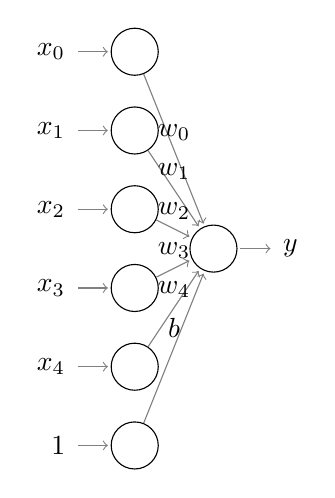
\begin{tikzpicture}[shorten >=1pt,->,draw=black!50, node distance=\layersep]
    \tikzstyle{every pin edge}=[<-,shorten <=1pt]
    \tikzstyle{neuron}=[circle,draw=black,minimum size=17pt,inner sep=0pt]
    \tikzstyle{input neuron}=[neuron];
    \tikzstyle{output neuron}=[neuron, fill=red!50];
    \tikzstyle{hidden neuron}=[neuron];
    \tikzstyle{annot} = [text width=4em, text centered]

    % Draw the input layer nodes
    \foreach \name / \y in {0,...,4}
    % This is the same as writing \foreach \name / \y in {1/1,2/2,3/3,4/4}
        \node[input neuron,pin=left:$x_\y$] (I-\name) at (0,-\y) {};
    \node[input neuron,pin=left:1] (I-5) at (0,-5) {};

    % Draw the output layer node
    \node[hidden neuron,pin={[pin edge={->}]right:$y$}] (O) at (\layersep, -2.5) {};

    % Connect every node in the input layer with every node in the
    % hidden layer.
    % \foreach \source in {1,...,5}
        % \draw(I-\source) edge (O) node[above, midway] {$w_\source$};
    \foreach \source in {0,...,4}
        \draw[->] (I-\source) -- (O) node[above,midway] {$w_\source$};
    \draw[->] (I-5) -- (O) node[above,midway] {$b$};

    % Annotate the layers
    % \node[annot,above of=I-1, node distance=1cm] (il) {Input Layer};
    % \node[annot,right of=hl] {Output layer};
\end{tikzpicture}
% End of code

  \mycaption{A single neuron}{The neuron is composed of inputs $x_i$, weights
    $w_i$ (and a bias term), as well as an activation function. Typical activation
    functions include the sigmoid function, tanh function and the ReLU}
  \label{fig:ch2:singlelayer}
\end{figure}

The neuron, shown in \autoref{fig:ch2:singlelayer} is the core building block of
Neural Networks. It takes the dot product between an input vector $\vec{x} \in
\reals[D]$ and a weight vector $\vec{w}$, before applying a chosen nonlinearity,
$g$. I.e.
%
\begin{equation}
  y = g(\langle\vec{x}, \vec{w}\rangle) = g\left(\sum_{i=0}^{D} x_i w_i \right) 
\end{equation}
%
where we have used the shorthand $b=w_0$ and $x_0 = 1$. Also note that we will
use the neural network common practice of calling the \emph{weights} $w$,
compared to the parameters $\theta$ we have been discussing thus far.

Typical nonlinear functions $g$ are the sigmoid function (already presented in 
\eqref{eq:ch2:sigmoid}), but also common are the tanh and ReLU functions:
\begin{eqnarray}
  \F{tanh}(x) &=& \frac{e^{x} - e^{-x}}{e^{x} + e^{-x}} \label{eq:ch2:tanh}\\
  \F{ReLU}(x) &=& \max (x, 0) \label{eq:ch2:relu}
\end{eqnarray}

See \autoref{fig:ch2:nonlinearities} for plots of these. The original Rosenblatt
perceptron \cite{rosenblatt_perceptron:_1958} used the Heaviside function
$\F{H}(x) = \mathbb{I}(x > 0)$. % The sigmoid nonlinearity
% naturally arises when we want to do classification with class labels $\{0,1\}$,
% as does the tanh function for classification with class labels $\{-1, 1\}$. The
% ReLU however is used more often in deeper architectures
% \cite{nair_rectified_2010}.

Note that if $\langle\vec{w}, \vec{w}\rangle = 1$ then $\langle\vec{x},
\vec{w}\rangle$ is the distance from the point $\vec{x}$ to the hyperplane with
normal $\vec{w}$. With general $\vec{w}$ this can be thought of as a scaled
distance. Thus, the weight vector $\vec{w}$ defines a hyperplane in $\reals[D]$
which splits the space into two. The choice of nonlinearity then affects how
points on each side of the plane are treated. For a sigmoid, points far below
the plane get mapped to 0 and points far above the plane get mapped to 1 (with
points near the plane having a value of 0.5). For tanh nonlinearities, these
points get mapped to -1 and 1. For ReLU nonlinearities, every point below the
plane ($\langle\vec{x}, \vec{w}\rangle < 0$) gets mapped to zero and every point
above the plane keeps its inner product value. 

Nearly all modern neural networks use the ReLU nonlinearity and it has
been credited with being a key reason for the recent surge in deep learning
success \cite{glorot_deep_2011, nair_rectified_2010}. In particular:
\begin{enumerate}
\item It is less sensitive to initial conditions as the gradients that
  backpropagate through it will be large even if $x$ is large. A common
  observation of sigmoid and tanh non-linearities was that their learning would
  be slow for quite some time until the neurons came out of saturation, and then
  their accuracy would increase rapidly before levelling out again at
  a minimum~\citep{glorot_understanding_2010}. The ReLU, on the other hand, has
  constant gradient.
\item It promotes sparsity in outputs, by setting them to a hard 0. Studies
  on brain energy expenditure suggest that neurons encode information in
  a sparse manner. \citet{lennie_cost_2003} estimates the percentage of
  neurons active at the same time to be between 1 and 4\%. Sigmoid and tanh
  functions will typically have \emph{all} neurons firing, while 
  the ReLU can allow neurons to fully turn off.
\end{enumerate}

\begin{figure}
    \qquad
    \section{Wavelet Based Nonlinearities and Multiple Gain Layers}
So far we have only considered doing the mixing operations in the wavelet
domain. This is a good starting point, and it is nice to see that we can do
apply the gain layer that
preserve some of the nice properties of the $\DTCWT$. Let us call the layer
considered so far a \textbf{first order gain layer}. Recall this is where a
$\DTCWT$ is done, followed by a single linear convolution and then straight away
returning to the pixel domain with the inverse $\DTCWT$. While it is good to see
that it is possible to do and even achieves some benefit over a convolutional
layer, the proposed layer \eqref{eq:ch6:end2end} can be implemented in the pixel domain
as a single convolution.

It would be particularly interesting if we could find a sensible nonlinearity to
do in the wavelet domain. This would mean it would be no longer possibile to do the
gain layer in the pixel domain. Further, we could then do multiple mixing
stages in the wavelet domain before returning to the pixel domain.

But what sensible nonlinearity to use? Two particular options are good initial
candidates:
\begin{enumerate}
  \item The ReLU: this is a mainstay of most modern neural networks and has
    proved invaluable in the pixel domain. Perhaps its sparsifying properties
    will work well on wavelet coefficients too. 
  \item Soft thresholding: a technique commonly applied to wavelet
    coefficients for denoising and compression. Many proponents of compressed
    sensing and dictionary learning even like to compare soft thresholding to a
    two sided ReLU \cite{papyan_theoretical_2018, papyan_convolutional_2016}.
\end{enumerate}

In this section we will look at each, see if they add to the first order gain
layer, and see if they open the possibility of having multiple layers in the
wavelet domain. 

\subsection{ReLUs in the Wavelet Domain}
A ReLU could be applied to the real lowpass coefficients with ease, but it does
not generalize so easily to complex coefficients. One option could be to apply
it independently to the real and imaginary coefficients, effectively only
selecting one quadrant of the complex plane.

One potential problem with this is
that applying a ReLU independently to the real and imaginary components


    \quad
    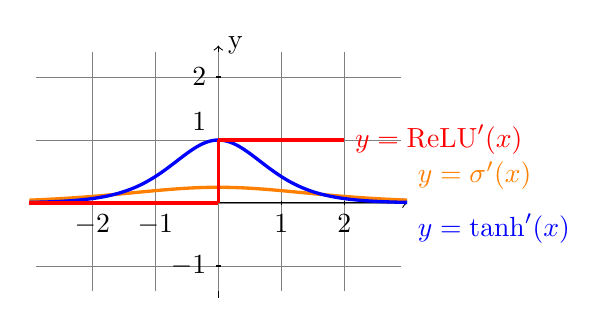
\begin{tikzpicture}[scale=0.8]
  % Draw axes
  \draw[->] (-3,0) -- (3,0);
  \draw[->] (0,-1.5) -- (0,2.5) node[right] {y};

  % Draw gridlines
  \draw[step=1cm,gray,very thin] (-2.9,-1.4) grid (2.9, 2.4);

  \foreach \x in {-2,-1,1,2}
    \draw (\x cm,1pt) -- (\x cm,-1pt) node[anchor=north] {$\x$};
  \foreach \y in {-1,  2}
    \draw (1pt, \y cm) -- (-1pt, \y cm) node[anchor=east] {$\y$};
  \draw (1pt, 1 cm) -- (-1pt, 1 cm) node[anchor=south east] {$1$};

  % Draw sigmoid
  \draw[orange, very thick, domain=-3:3, samples=200] plot (\x, {(exp(-\x)/(1+exp(-\x))^2})
    node[above right] {$y=\sigma'(x)$};

  % Draw Tanh
  \draw[blue, very thick, domain=-3:3, samples=200] plot (\x, {1 - ((exp(\x)-exp(-\x))/(exp(\x)+exp(-\x)))^2})
    node[below right] {$y=\tanh'(x)$};

  % Draw ReLU
  \draw[red, very thick, domain=-3:0, samples=5] plot (\x, {0});
  \draw[red, very thick] (0, 0) -- (0, 1);
  \draw[red, very thick, domain=0:2, samples=5] plot (\x, {1}) node[right]
    {$y=\F{ReLU}'(x)$};

\end{tikzpicture}


  \centering
  \mycaption{Common Neural Network nonlinearities and their gradients}{The sigmoid, tanh and ReLU
  nonlinearities are commonly used activation functions for neurons. Note the
  different properties. In particular, the tanh and sigmoid have the nice
  property of being smooth but can have saturation when the input is either
  largely positive or largely negative, causing little gradient to flow back
  through it. The ReLU does not suffer from this problem, and has the additional
  nice property of setting values to exactly 0, making a sparser output
  activation.}
  \label{fig:ch2:nonlinearities}
\end{figure}

\subsection{Multilayer Perceptrons}
As mentioned in the previous section, a single neuron can be thought of as a
separating hyperplane with an activation that maps the two halves of the space
to different values. Such a linear separator is limited, and famously cannot
solve the XOR problem \cite{minsky_perceptrons:_1988}. Fortunately, adding a
single hidden layer like the one shown in \autoref{fig:ch2:hidden} can change
this, and it is provable that with an infinitely wide hidden layer, a neural
network can approximate any function \cite{hornik_multilayer_1989,
cybenko_approximation_1989}. 

The forward pass of such a network with one hidden layer of $H$ units is:
%
\begin{eqnarray}
  h_i & = & g\left(\sum_{j=0}^{D} x_j w_{ij}^{(1)}\right) \\
  y & = & \sum_{k=0}^{H} h_k w^{(2)}_{k}
\end{eqnarray}
%
where $w^{(l)}$ denotes the weights for the $l$-th layer, of which
\autoref{fig:ch2:hidden} has 2. Note that these individual layers are often
called \emph{fully connected} as each node in the previous layer affects every
node in the next.

If we were to expand this network to have $L$ such fully connected layers, we
could rewrite the action of each layer in a recursive fashion:
%
\begin{eqnarray}
  Y^{(l+1)} &=& W^{(l+1)}X^{(l)}  \label{eq:ch2:fc1}\\
  X^{(l+1)} &=& g\left(Y^{(l+1)}\right) \label{eq:ch2:fc2} 
\end{eqnarray}
where $W$ is now a weight matrix, acting on the vector of previous layer's
outputs $X^{(l)}$. As we are now considering every layer an input to the next
stage, we have removed the $h$ notation, and added the superscript $(l)$ to
define the depth. $X^{(0)}$ is the network input and $Y^{(L)}$ is the network
output. Let us say that the output has $C$ nodes, and a hidden layer $X^{(l)}$
has $C_l$ nodes.

\begin{figure}[t]
  \centering
  \input{\imgpath/network_mlp}
  \mycaption{Multi-layer perceptron}{Expanding the single neuron from 
  \autoref{fig:ch2:singlelayer} to a network of neurons. The internal
  representation units are often referred to as the \emph{hidden layer} as they
  are an intermediary between the input and output.}
  \label{fig:ch2:hidden}
\end{figure}

\subsection{Backpropagation}
It is important to truly understand backpropagation when designing neural
networks, so we describe the core concepts now for a neural network with
$L$ layers.

The delta rule, initially designed for networks with no hidden layers 
\cite{widrow_neurocomputing:_1988}, was expanded to what we now consider
\emph{backpropagation} in \cite{rumelhart_parallel_1986}. While backpropagation
is conceptually just the application of the chain rule, Rumelhart, Hinton, and
Williams successfully updated the delta rule to networks with hidden layers,
laying a key foundational step for deeper networks. 

With a deep network, calculating $\dydx{J}{w}$ may not seem
particularly obvious if $w$ is a weight in one of the earlier layers. We need
to define a rule for updating the weights in all $L$ layers of the network,
$W^{(1)}, W^{(2)}, \ldots W^{(L)}$ however, only the final set $W^{(L)}$ are
connected to the objective function $J$. 

\subsubsection{Regression Loss}
Let us start with writing down the derivative of $J$ with respect to the network
output $Y^{(L)}$ using the regression objective function \eqref{eq:ch2:mle_reg}. 
As we now have two superscripts,
one for the sample number and one for the layer number, we combine them into a
tuple of superscripts. 
\begin{eqnarray}
  \dydx{J}{Y^{(L)}} &= & \dydx{}{Y^{(L)}} \left( \frac{1}{N}\sum_{n=1}^{N_b}\frac{1}{2} \left(y^{(n)} - Y^{(L, n)}\right)^2\right) \\
                    &=& \frac{1}{N}\sum_{n=1}^{N_b} \left(Y^{(L, n)} - y^{(n)} \right) \\
                    &=& e \in \reals \label{eq:ch2:reg_b1}
\end{eqnarray}
where we have used the fact that for the regression case, $y^{(n)}, Y^{(L,n)}
\in \reals$. 

\subsubsection{Classification Loss}
For the classification case \eqref{eq:ch2:mle_class}, let us keep the output of
the network $Y^{(L,n)} \in \reals[C]$ and define an intermediate value $\hat{y}$ the
softmax applied to this vector $\hat{y}^{(n)}_c = \sigma_c\left(Y^{(L, n)}\right)$.
Note that this is a vector valued function going from $\reals[C] \rightarrow
\reals[C]$ so has a jacobian matrix $S_{ij} = \dydx{\hat{y}_i}{Y^{(L)}_j}$ with
values:
\begin{equation}
  S_{ij} = \begin{cases}
    \sigma_i (1-\sigma_j) & \text{if $i=j$}\\
    -\sigma_i \sigma_j & \text{if $i\neq j$}\\
  \end{cases}
\end{equation}

Now, let us return to \eqref{eq:ch2:mle_class} and find the derivative of the
objective function to this intermediate value $\hat{y}$:
\begin{eqnarray}
  \dydx{J}{\hat{y}} &= & \dydx{}{\hat{y}} \left( \frac{1}{N}\sum_{n=1}^{N_b} \sum_{c=1}^C 
  y^{(n)}_c \log \hat{y}^{(n)}_c \right) \\
  &=& \frac{1}{N}\sum_{n=1}^{N_b} \sum_{c=1}^C \frac{y^{(n)}_c}{\hat{y}^{(n)}_c} \\
  &=& d \in \reals[C] \label{eq:ch2:class_b1}
\end{eqnarray}
Note that unlike \eqref{eq:ch2:reg_b1}, this derivative is vector valued. To
find $\dydx{J}{Y^{(L)}}$ we use the chain rule. It is easier to find the
partial derivative with respect to one node in the output first, and then expand
from here. I.e.:

\begin{eqnarray}
  \dydx{J}{Y^{(L)}_j} &=& \sum_{i=1}^C \dydx{J}{\hat{y}_i}\dydx{\hat{y}_i}{Y^{(L)}_j} \\
                      &=& S_i^T d
\end{eqnarray}
where $S_i$ is the $i$th column of the jacobian matrix $S$. It becomes clear now
that to get the entire vector derivative for all nodes in $Y^{(L)}$, we must
multiply the transpose of the jacobian matrix with the error term from
\eqref{eq:ch2:class_b1}:
\begin{equation}
  \dydx{J}{Y^{(L)}} = S^T d
\end{equation}

\subsubsection{Final Layer Weight Gradient} \label{sec:ch2:weight}
Let us continue by assuming $\dydx{J}{Y^{(L)}}$ is vector valued as was the case
with classification. For regression, it is easy to set $C=1$ in the following to
get the necessary results. Additionally for clarity, we will drop the layer
superscript in the intermediate calculations.

We call the gradient for the final layer weights the \emph{update} gradient. 
It can be computed by the chain rule again:
\begin{eqnarray}
  \dydx{J}{W_{ij}} &=& \dydx{J}{Y_i} \dydx{Y_i}{W_{ij}} + 2\lambda W_{ij} \\
  &=& \dydx{J}{Y_i} X_j + 2\lambda W_{ij}
\end{eqnarray}
where the second term in the above two equations comes from the regularization
loss that is added to the objective. The gradient of the entire weight matrix is 
then:
\begin{eqnarray}
  \dydx{J}{W^{(L)}} &=& \dydx{J}{\hat{y}} X^T +2\lambda W \\
   &=& S^T d \left(X^{(L-1)}\right)^T + 2\lambda W^{(L)} \in \reals[C \x C_{L-1}]
\end{eqnarray}

\subsubsection{Final Layer Passthrough Gradient} \label{sec:ch2:passthrough}
Additionally, we want to find the \emph{passthrough} gradients of the final
layer $\dydx{J}{X^{(L-1)}}$. In a similar fashion, we first find the gradient
with respect to individual elements in $X^{(L-1)}$ before generalizing to the
entire vector:
\begin{eqnarray}
  \dydx{J}{X_i} &=& \sum_{j=1}^{C} \dydx{J}{Y_j} \dydx{Y_j}{X_i} \\
                &=& \sum_{j=1}^{C} \dydx{J}{Y_j} W_{j,i} \\
                &=& W_{i}^T\dydx{J}{Y} \\
\end{eqnarray}
where $W_i$ is the $i$th column of $W$. Thus
\begin{eqnarray}
  \dydx{J}{X^{(L-1)}} &=& \left(W^{(L)}\right)^T \dydx{J}{Y^{(L)}} \\
                      &=& \left( W^{(L)} \right)^T S^T d
\end{eqnarray}
This passthrough gradient then can be used to update the next layer's weights by
repeating \autoref{sec:ch2:weight} and \autoref{sec:ch2:passthrough}.

\subsubsection{General Layer Update}
The easiest way to handle this flow of gradients, and the basis for most
automatic differentiation packages, is the block definition shown in
\autoref{fig:ch2:block_form}. For all neural network components (even if they do
not have weights), the operationg must not only be able to calculate the forward 
pass $y=f(x, w)$ given weights $w$ and inputs $x$, but also calculate the
\emph{update} and \emph{passthrough} gradients $\dydx{J}{w}, \dydx{J}{x}$ given
an input gradient $\dydx{J}{y}$. The input gradient will have the same shape as
$y$ as will the update and passthrough gradients match the shape of $w$ and $x$.
This way, gradients for the entire network cam be computed in an iterative
fashion starting at the loss function and moving backwards.

\begin{figure}
  \centering
  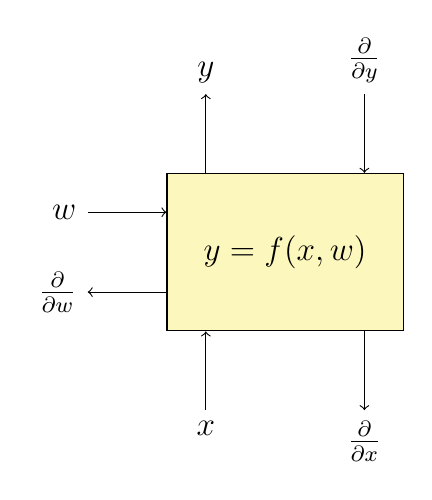
\begin{tikzpicture}[every node/.style={node font=\large}]
\definecolor{mycolor}{RGB}{252,247,189};
\pgfmathsetmacro{\EDGE}{.5}
\node [fill=mycolor, draw, minimum width=3cm, minimum height=2cm] (block) at (1,1) {$y=f(x,w)$};
\coordinate[right=\EDGE of block.south west] (xin);
\coordinate[left=\EDGE of block.south east] (dxin);
\coordinate[below=\EDGE of block.north west] (win);
\coordinate[above=\EDGE of block.south west] (dwin);
\coordinate[right=\EDGE of block.north west] (yin);
\coordinate[left=\EDGE of block.north east] (dyin);
\draw[<-] (xin) -- +(0,-1) node[below] {$x$};
\draw[->] (dxin) -- ++(0,-1) node[below] {$\dydx{\logloss}{x}$};
\draw[<-] (win) -- ++(-1,0) node[left] {$w$};
\draw[->] (dwin) -- ++(-1,0) node[left] {$\dydx{\logloss}{w}$};
\draw[->] (yin) -- ++(0,1) node[above] {$y$};
\draw[<-] (dyin) -- ++(0,1) node[above] {$\dydx{\logloss}{y}$};
\end{tikzpicture}

  \mycaption{General block form for autograd}{All neural network functions
  need to be able to calculate the forward pass $y=f(x,w)$ as well as the 
  update and passthrough gradients $\dydx{J}{w}, \dydx{J}{x}$. Backpropagation
  is then easily done by allowing data to flow backwards through these blocks
  from the loss.}
  \label{fig:ch2:block_form}
\end{figure}

\section{Convolutional Neural Networks}
Convolutional Neural Networks (CNNs) are a special type of of Neural Network where the
weights of the fully connected layer are shared across the layer. 
In this way, a neuron at a given layer is only affected by
nodes from the previous layer in a given neighbourhood rather than every node.

First popularized in 1998 by LeCun et. al in \cite{lecun_gradient-based_1998},
the convolutional layer was introduced to build invariance with respect to
translations, as well as reduce the parameter size of early neural networks for
pattern recognition. The idea of having a locally receptive field had already
been shown to be a naturally occurring phenomen by Hubel and Wiesel
\cite{hubel_receptive_1962}. They did not become popular immediately, and
another spatially based keypoint extractor, SIFT \cite{lowe_distinctive_2004},
was the mainstay of detection systems until the AlexNet CNN
\cite{krizhevsky_imagenet_2012} won the 2012 ImageNet challenge
\cite{russakovsky_imagenet_2014} by a large margin over the next competitors who
used SIFT and Support Vector Machines \cite{cortes_support-vector_1995}. This
CNN had 5 convolutional layers followed by 3 fully connected layers.

We will briefly describe the convolutional layer, as well as many other layers
that have become popular in the past few years.

\subsection{Convolutional Layers}
In the presentation of neural networks so far, we have considered column vectors 
$X^{(l)},Y^{(l)} \in \reals[C_{l}]$. Convolutional layers for image analysis
have a different format. In particular, the spatial component of the input is
preserved. 

Let us first consider the definition of 2-D convolution for single channel
images:
\begin{eqnarray}
  y[\nn] = (x\conv h)[\nn] &=& \sum_{\mathbf{k}} x[\mathbf{k}]h[\nn-\mathbf{k}] \label{eq:ch2:conv1}\\
                      &=& \sum_{k_1, k_2} x[k_1,k_2]h[n_1-k_1, n_2-k_2]
\end{eqnarray}
where the sum is done over the support of $h$. For an input $x\in \reals[H\x W]$
and filter $h\in \reals[K_1\x K_2]$ the output has spatial support $y\in
\reals[H+K_1-1 \x W+K_2-1]$. 

In the context of convolutional layers, this filter $h$ is a \emph{matched filter} 
that gives its largest output when the input contains $h$. If the input has
shapes similar to $h$ in many locations, each of these locations in $y$ will
also have large outputs. 

It is not enough to only have a single matched filter, often we would like to
have a bank of them, each sensitive to different shapes. For example, if $h_1$
was sensitive to horizontal edges, we may also want to detect vertical and
diagonal edges. Without specifying what each of the filters do, we can however
specify that we would like to detect $C$ different shapes over the spatial
extent of an input.

This then means that we have $C$ output channels:
\begin{eqnarray*}
  y_1[\nn] &=& (x \conv h_1)[\nn] \\
  y_2[\nn] &=& (x \conv h_1)[\nn] \\
           &\vdots & \\
  y_C[\nn] &=& (x \conv h_1)[\nn] 
\end{eqnarray*}

If we stack red, green and blue input channels on top of each other, we have a 
3-dimensional array $x \in \reals[C\x H\x W]$ with $C=3$.\footnote{In deep 
learning literature, there is not consensus about whether to stack the outputs
with the channel first ($\reals[C\x H\x W]$) or last ($\reals[H\x W\x C]$). The
latter is more common in Image Processing for colour and spectral images,
however the former is the standard for the deep learning framework we use --
PyTorch \cite{paszke_automatic_2017}, so we use this in this thesis.} 
In a CNN layer, each filter $h$ is 3 dimensional with spatial extent exactly
equal to $C$. The \emph{convolution} is done over the remaining two dimensions
and the $C$ outputs are summed at each pixel location. This makes
\eqref{eq:ch2:conv1}:
\begin{eqnarray}
  y[\nn] &=& \sum_{c=1}^C \sum_{\mathbf{k}} x[\mathbf{k}]h[c, \nn-\mathbf{k}]
  \label{eq:ch2:conv2}
\end{eqnarray}

Again, we would like to have many matched filters to find different shapes in
the previous layer, so we repeat \autoref{eq:ch2:conv2} $F$ times and stack the
output to give $y \in \reals[F \x H\x W]$: 
%
\begin{equation}
  y[f, \nn] &=& \sum_{c=1}^C \sum_{\mathbf{k}} x[c, \mathbf{k}]h_f[c, \nn-\mathbf{k}]
  \label{eq:ch2:conv3}
\end{equation}

After a convolutional layer, we can then apply a pointwise nonlinearity $g$ to
each output location in $y$. Revisiting \eqref{eq:ch2:fc1} and \eqref{eq:ch2:fc2}, we can 
rewrite this for a convolutional layer at depth $l$ with $C_l$ input and
$C_{l+1}$ output channels:
\begin{eqnarray}
  Y^{(l+1)}[f, \nn] &=& \sum_{c=1}^{C_l} X^{(l)}[c, \nn] \conv h^{(l)}_f[c, \nn] \qquad 
    \text{for } 1 \leq f \leq C_{l+1} \label{eq:ch2:conv4}\\
  X^{(l+1)}[f, \nn] &=& g\left(Y^{(l)}[f, \nn]\right)
\end{eqnarray}
This is shown in \autoref{fig:ch2:conv_layer}.

\begin{figure}
  \centering
    \begin{tikzpicture}[%
    path image/.style={
      path picture={
        \node at (path picture bounding box.center) {
          \includegraphics[height=2.0cm]{#1}
        };
      }
    }, 
    path pic/.style={
      path picture={
        \node at (path picture bounding box.center) {
          \includegraphics[height=1.2cm]{#1}
        };
      }
    }, 
    path pic2/.style={
      path picture={
        \node at (path picture bounding box.center) {
          \includegraphics[height=0.8cm]{#1}
        };
      }
    }, 
    scale=0.8]

    \tikzcuboid{
    shiftx=0cm,
    shifty=-1cm,
    scale=0.5,
    dimx=2, dimy=2, dimz=12,
    densityx=2, densityy=2, densityz=2,
    dimxval=W, dimyval=H, dimzval=C_l,
    drawxdims=true, drawydims=true, drawzdims=true,
    front/.style={draw=blue!50!white,fill=blue!50!white},%
    right/.style={draw=blue!50!white,fill=blue!50!white},%
    top/.style={draw=blue!50!white,fill=blue!50!white},%
    shade=false,
    emphedge=true,
    shadeopacity=0,
    emphstyle/.style={rounded corners=0.2pt,line width=0.3mm},
    }
    \draw (1.6, 1.7, 0) node {\large{$x^{(l)}$}};
    \draw (5.5, 2.9, 0) node {\large{$h^{(l+1)}$}};
    \draw (9.7, 1.6, 0) node {\large{$y^{(l+1)}$}};
    \draw (13.7, 1.6, 0) node {\large{$x^{(l+1)}$}};
    \draw (2.2, -.8, 0) node {\Large{$\conv$}};

    \tikzcuboid{
    shiftx=4cm,
    shifty=1cm,
    scale=0.5,
    dimx=.7, dimy=.7, dimz=12,
    dimxval=k_w, dimyval=k_h,
    densityx=5, densityy=5, densityz=2,
    drawxdims=false,
    drawydims=false,
    drawzdims=false,
    front/.style={draw=red!50!white,fill=red!50!white},%
    right/.style={draw=red!50!white,fill=red!50!white},%
    top/.style={draw=red!50!white,fill=red!50!white},%
    }
    \tikzcuboid{
    shifty=0cm,
    }
    \tikzcuboid{
    shifty=-2.0cm,
    scale=0.5,
    drawxdims=true,
    drawydims=true,
    drawzdims=true,
    dimzval=C_l,
    }
    \draw (3.2, -1.7, -2.8) node {$\vdots$};
    \draw [<->] (3.3, 0.1, -6) -- (3.3, -3.2, -6) node[near start, right] {$C_{l+1}$};
    \draw [->, fill=gray!30,ultra thick] (5, -1.5, -2.5) -- (6, -1.5, -2.5);

    \tikzcuboid{
    shiftx=8cm,
    shifty=-1cm,
    scale=0.5,
    dimx=2, dimy=2, dimz=10,
    densityx=4, densityy=4, densityz=2,
    dimzval=C_{l+1},
    drawzdims=true,
    drawxdims=false,
    drawydims=false,
    front/.style={draw=blue!50!white,fill=blue!50!white},%
    right/.style={draw=blue!50!white,fill=blue!50!white},%
    top/.style={draw=blue!50!white,fill=blue!50!white},%
    }
    \draw [->, fill=gray!30,ultra thick] (9, -1.5, -2.5) -- (10, -1.5, -2.5)
      node[midway, above] {$\sigma$};

    \tikzcuboid{
    shiftx=12cm,
    shifty=-1cm,
    scale=0.5,
    dimx=2, dimy=2, dimz=10,
    densityx=4, densityy=4, densityz=2,
    drawzdims=true,
    dimzval=C_{l+1},
    drawxdims=false,
    drawydims=false,
    drawzdims=false,
    front/.style={draw=blue!50!white,fill=blue!50!white},%
    right/.style={draw=blue!50!white,fill=blue!50!white},%
    top/.style={draw=blue!50!white,fill=blue!50!white},%
    }

  \end{tikzpicture}

  \mycaption{A convolutional layer}{A convolutional layer followed by a
  nonlinearity $g$. The previous layer's activations are convolved with a bank
  of $C_{l+1}$ filters, each of which has spatial size $k_h\x k_w$ and depth
  $C_l$. Note that there is no convolution across the channel dimension. Each
  filter produces one output channel in $y^{(l+1)}$.}
  \label{fig:ch2:conv_layer}
\end{figure}

\subsubsection{Padding and Stride}
Regular 2-D convolution expands the input from size $H\x W$ to $(H+K_H-1)\x
(W+K_W-1)$. In convolutional layers in neural networks, it is often desirable
and common to have the same output size as input size. This is achieved by
taking the central $H\x W$ outputs. We call this \emph{same-size convolution}.
Another option commonly used is to only evaluate the kernels where they fully
overlap the input signal, causing a reduction in the output size to $(H-K_H+1)
\x (W-K_W+1)$. This is called \emph{valid convolution} and was used in the
original LeNet-5 \cite{lecun_gradient-based_1998}.

Signal extension is by default \emph{zero padding}, and most deep learning
frameworks have no ability to choose other padding schemes as part of their
convolution functions. Other padding such as \emph{symmetric padding} can be
achieved by expanding the input signal before doing a valid convolution.

Stride is a commonly used term in deep learning literature. A stride of 2 means
that we evaluate the filter kernel at every other sample point. In signal
processing, this is simply called decimation.

\subsubsection{Gradients}
To get the update and passthrough gradients for the convolutional layer we will need to expand
\eqref{eq:ch2:conv4}. Again we will drop the layer superscripts for clarity. For
simplicity, let us assume that the convolutional filters are square and only have
support in the region $a \leq n_1, n_2 \leq b$

\begin{equation}
  Y[f, n_1, n_2] &=& \sum_{c=1}^C \sum_{k_1=a}^{b} \sum_{k_2=a}^b x[c, k_1, k_2]
  h_f[c, n_1-k_1, n_2-k_2] \label{eq:ch2:conv5}
\end{equation}

\subsection{Pooling}
  Typically following a convolutional layer (but not strictly), activations are subsampled with
  max pooling. Pooling adds some invariance to shifts smaller than the pooling
  size at the cost of information loss. For this reason, small pooling is
  typically done often $2\x 2$ or $3\x 3$, and the invariance to larger shifts
  comes after multiple pooling (and convolutional) layers.
  
  While initial designs of max pooling would do it in non-overlapping regions, 
  AlexNet used $3\x 3$ pooling with stride 2 in their breakthrough design,
  quoting that it gave them an increase in accuracy of roughly $0.5\%$ and
  helped prevent their network from `overfitting'. More recent networks will
  typically employ either this or the original $2\x 2$ pooling with stride 2,
  see \autoref{fig:ch2:maxpool}. A review of pooling methods in
  \citep{mishkin_systematic_2016} found them both to perform equally well.
  
  \begin{figure}
    \centering
    \input{\imgpath/pooling_both}
    \mycaption{Max vs Average $2\x 2$ pooling}{}
    \label{fig:ch2:maxpool}
  \end{figure}

\subsubsection{Batch Normalization}
      Batch normalization proposed only very recently in
      \citep{ioffe_batch_2015} is a conceptually simpler technique. Despite
      that, it has become quite popular and has been found to be very useful.
      At its core, it is doing what standard normalization is doing, but also
      introduces two learnable parameters --- scale ($\gamma$) and offset
      ($\beta$). \eqref{eq:ch2:normalization} becomes:
      \begin{equation}
        \tilde{z}(u_1,u_2,d) = \gamma\frac{z-E[z]}{\sqrt{Var[z]}} + \beta 
				\label{eq:ch2:batch_normalization}
      \end{equation}
      These added parameters make it a \emph{renormalization} scheme, as instead of
      centring the data around zero with unit variance, it can be centred
      around an arbitrary value with arbitrary variance. S etting
      $\gamma = \sqrt{Var[z]}$ and $\beta = E[z]$, we would get the identity
      transform. Alternatively, setting $\gamma = 1$ and $\beta = 0$ (the
      initial conditions for these learnable parameters), we get standard
      normalization.
      
      The parameters $\gamma$ and $\beta$ are learned through backpropagation.
      As data are usually processed in batches, the gradients for $\gamma$ and
      $\beta$ are calculated per sample, and then averaged over the whole
      batch.

      From \autoref{eq:ch2:batch_normalization}, let us briefly use the hat
      notation to represent the standard normalized input:
      $\hat{z} = (z-E[z])/\sqrt{Var[z]}$, then:
      \begin{eqnarray}
        \tilde{z}^{(i)} & = & \gamma \hat{z}^{(i)} + \beta \nonumber\\
        \frac{\partial \mathcal{L}}{\partial \gamma}& =&
        \frac{1}{N}\sum_{i=1}^{N} \frac{\partial
        \mathcal{L}^{(i)}}{\partial \tilde{z}^{(i)}} \cdot \hat{z}^{(i)} \\
        \frac{\partial \mathcal{L}}{\partial \beta}& =&
        \frac{1}{N}\sum_{i=1}^{N} \frac{\partial
        \mathcal{L}^{(i)}}{\partial \tilde{z}^{(i)}} 
      \end{eqnarray}

      Batch normalization layers are typically placed \emph{between} convolutional layers
      and non-linearities. I.e.,\ if $Wu+b$ is the output of a convolutional
      layer, and $z=g(Wu+b)$ is the output of the non-linearity, then with the
      batch normalization step, we have:
      \begin{eqnarray}
        z &=& g(BN(Wu+b)) \nonumber\\
          &=& g(BN(Wu))
      \end{eqnarray}
      Where the bias term was ignored in the convolutional layer, as it can be
      fully merged with the `offset' parameter $\beta$.

      This has particular benefit of removing the sensitivity of our network to
      our initial weight scale, as for scalar $a$,
      \begin{equation}
        BN(Wu) = BN((aW)u)
      \end{equation}
      It is also particularly useful for backpropagation, as an increase in
      weights leads to \emph{smaller} gradients \citep{ioffe_batch_2015}, making
      the network far more resilient to the problems of vanishing and exploding
      gradients:
      \begin{eqnarray}
        \frac{\partial BN((aW)u)}{\partial u} & = & \frac{\partial
        BN(Wu)}{\partial u} \nonumber\\
        \frac{\partial BN((aW)u)}{\partial (aW)} & = & \frac{1}{a} \cdot \frac{\partial
        BN(Wu)}{\partial W} 
      \end{eqnarray}


\section{Relevant Architectures}

\subsection{LeNet}
\subsection{AlexNet}
\subsection{VGG}
\subsection{Residual Networks}
  The current state of the art design introduced a clever novel feature called
  a residual unit\citep{he_deep_2015,he_identity_2016}. The inspiration for their design came from the difficulties
  experienced in training deeper networks. Often, adding an extra layer would
  \emph{decrease} network performance. This is counter-intuitive as the deeper
  layers could simply learn the identity mapping, and achieve the same
  performance.

  To promote the chance of learning the identity mapping, they define
  a residual unit, shown in \autoref{fig:ch2:residual_unit}. If a desired mapping
  is denoted $\mathcal{H}(x)$, instead of trying to learn this, they instead
  learn $\mathcal{F}(x) = \mathcal{H}(x) - x$. 
  \begin{figure}
    \centering
    % \includegraphics[width=0.5\textwidth]{images/residual_unit.png}
    \caption[The residual unit from ResNet]
          {A residual unit. The identity mapping is always present, and the
            network learns the difference from the identity mapping, $\mathcal{F}(x)$.
            Taken from \citep{he_deep_2015}.}
      \label{fig:ch2:residual_unit}
  \end{figure}


\subsection{old}
  Convolutional Neural Networks (CNNs) were initially introduced by \citet{lecun_backpropagation_1989} in
  \citep{lecun_backpropagation_1989}. Due to the difficulty of training and
  initializing them, they failed to be popular for more than two decades.  This
  changed in 2012, when advancements in pre-training with unsupervised networks
  \citep{bengio_greedy_2007}, the use of an improved non-linearity --- the Rectified Linear
  Unit, or ReLU, new regularization methods\citep{hinton_improving_2012}, and
  access to more powerful computers in graphics cards, or GPUs, allowed
  Krizhevsky, Sutskever and Hinton  to develop
  AlexNet\citep{krizhevsky_imagenet_2012}. This network nearly halved the
  previous state of the art's error rate.  Since then, interest in them has
  expanded very rapidly, and they have been successfully applied to object
  detection~\citep{ren_object_2015} and human pose estimation
  \citep{tompson_efficient_2015}. It would take a considerable amount of effort
  to document the details of all the current enhancements and tricks many
  researches are using to squeeze extra accuracy, so for the purposes of this
  report we restrict ourselves to their generic design, with some time spent
  describing some of the more promising enhancements. 
  
  We would like to make note of some of the key architectures
  in the history of CNNs, which we, unfortunately, do not have space to describe:
  \begin{itemize}
    \item Yann LeCun's LeNet-5~\citep{lecun_gradient-based_1998}, the state of the art
      design for postal digit recognition on the MNIST dataset.
    \item Google's GoogLeNet~\citep{szegedy_going_2015} achieved $6.67\%$ top-5
      error on ILSVRC2014, introducing the new `inception' architecture, which
      uses combinations of $1\x 1$, $3\x 3$ and $5\x 5$ convolutions.
    \item Oxford's VGG~\citep{simonyan_very_2014} --- $6.8\%$ and runner up in
      ILSVRC2014. The VGG design is very similar to AlexNet but was roughly
      twice as deep. More convolutional layers were used, but with smaller
      support --- only $3\x 3$. These were often stacked directly on top of
      each other without a non-linearity in between, to give the effective
      support of a $5\x 5$ filter.
    \item Microsoft Research's ResNet~\citep{he_deep_2015} achieved $4.5\%$ top-5 
      error and was the winner of ILSVRC2015. This network we will talk briefly
      about, as it introduced a very nice novel layer --- the residual layer.
  \end{itemize}

  Despite the many variations of CNN architectures currently being used, most
  follow roughly the same recipe (shown in \autoref{fig:ch2:cnn_generic}):
  \begin{figure}
    \centering
      % \includegraphics[width=\textwidth]{images/cnns.png}
      \caption[Standard CNN architecture]
              {Standard CNN architecture. Taken
              from~\citep{lecun_gradient-based_1998}}\label{fig:ch2:cnn_generic}
  \end{figure}

\subsection{Fully Connected Layers}\label{sec:ch2:cnn_fullyconnected}
  The convolution, pooling, and activation layers all
  conceptually form part of the \emph{feature extraction} stage of a CNN. One
  or more fully connected layers are usually placed after these layers to form
  the \emph{classifier}. One of the most elegant and indeed most powerful
  features of CNNs is this seamless connection between the \emph{feature
  extraction} and \emph{classifier} sub-networks, allowing the backpropagation
  of gradients through all layers of the entire network.

  The fully connected layers in a CNN are the same as those in a classical
  Neural Network (NN), in that they compute a dot product between their input
  vector and a weight vector:
  \begin{equation}
    z_i = \sum_{j} W_{ij}x_j
  \end{equation}
  The final output of the Fully Connected layer typically has the same number
  of outputs as the number of classes $C$ in the classification problem.


\section{The Fourier and Wavelet Transforms}

  Computer vision is an extremely difficult task. Pixel intensities in an image are
  typically not very informative in understanding what is in that image. 
  These values are sensitive to lighting conditions and camera configurations.
  It would be easy to take two photos of the same scene and get two vectors
  $x_1$ and $x_2$ that have a very large Euclidean distance, but to a human,
  would represent the same objects. What is most important in defining an image is
  difficult to define, however, some things are notably more important than
  others. In particular, the location or phase of the waves that make up an
  image is much more important than the magnitude of these waves, something
  that is not necessarily true for audio processing. A simple experiment to
  demonstrate this is shown in \autoref{fig:ch2:barbara_morph}. 
  \begin{figure}
    \centering
      \includegraphics[width=\textwidth]{\imgpath/barbara_mag_swap.png}
      \mycaption{Importance of phase over magnitude for images}
        {The phase of the Fourier transform of the first image is combined with
        the magnitude of the Fourier transform of the second image and
        reconstructed. Note that the first image has entirely won out and
        nothing is left visible of the cameraman.}
      \label{fig:ch2:barbara_morph}
  \end{figure}

\subsection{The Fourier Transform}
For a signal $f(t) \in L_2(\reals)$ (square summable signals), the \emph{Fourier
transform} is defined as:
\begin{equation}
  F(\omega) = \int_{-\infty}^{\infty} f(t) e^{-j\omega t} dt
\end{equation}
This can be extended to two dimensions for signals $f(\xy) \in L_2(\reals[2])$:
\begin{equation}
  F(\ww) = \int_{-\infty}^{\infty}\int_{-\infty}^{\infty} f(\xy) e^{-j\ww^t \xy} d\xy = \langle f(\xy),\ e^{j\ww^t \xy} \rangle
\end{equation}

The Fourier transform is an invaluable signal expansion, as viewing a signal in
the frequency space offers many insights, as well as affording many very useful
properties (most notably the efficiency of convolution as a product of Fourier
transforms). While it is a mainstay in signal processing, 
it can be a poor
feature descriptor due to the infinite support of its basis functions - the
complex sinusoids $e^{j\ww^t u}$. If
a single pixel changes in the input it can change all of the
Fourier coefficients. As natural images are generally non-stationary, we need
to be able to isolate frequency components in local regions of an image, and
not have this property of global dependence. To achieve a more local Fourier
transform we can use the short time (or short space) Fourier Transform (STFT) or the
continuous wavelet transform (CWT). The two are very similar and mainly differ in the
way they handle the concept of `scale'. We will only discuss the CWT in this review, 
but for an excellent comparison of the two, we recommend \cite[Chapter~1]{antoine_two-dimensional_2004}.

% The Fourier transform does have one nice property, however, in that the magnitude of
% Fourier coefficients are invariant to global translations, a nuisance
% variability. We explore this theme more in our review of the Scattering
% Transform by \Mallat in \autoref{ch:scatternets}.

\subsection{The Continuous Wavelet Transform}
The \emph{continuous wavelet transform}, like the Fourier Transform, can be used
to decompose a signal into its frequency components. Unlike the Fourier
transform, these frequency components can be localized in space. To
achieve this, we need a bandpass filter, or \emph{mother wavelet}
$\psitd$\footnote{We use upright $\psiod, \phiod$ to distinguish 1-D wavelets
from their 2-D counterparts $\psitd, \phitd$} such that:
\begin{equation}
  \int_{-\infty}^{\infty} \psitd(\xy) d\xy = \Psi(0) = 0\label{eq:ch2:admissibility}
\end{equation}
Any function that has sufficient decay of energy with frequency and satisfies
\eqref{eq:ch2:admissibility}, is said to satisfy the \emph{admissibility condition}.

As we are working in 2-D for image processing, consider rotations, dilations, and 
shifts of this function by $\theta\in [0,2\pi],\ a>0,\ \bmu{b} \in \reals[2]$ respectively, where 
\begin{align}
  \text{Rotation: } & R_{\theta}x(\xy) = x(r_{-\theta}\xy) \label{eq:ch2:rot}\\
  \text{Dilation: } & D_{a}x(\xy) = \frac{1}{a} x\left(\frac{\xy}{a}\right), \quad a>0 \label{eq:ch2:di}\\
  \text{Translation: } & T_{\bmu{b}}x(\xy) = x(\xy - \bmu{b}) \label{eq:ch2:tr} 
\end{align}
where $r_\theta$ is the 2-D rotation matrix. Now consider shifts, scales and
rotations of our bandpass filter 
\begin{equation}
  \psitd_{\bmu{b},a, \theta}(\xy) = \frac{1}{a}\psitd \left(\frac{r_{-\theta}\left(\xy -
  \bmu{b}\right)}{a} \right) \label{eq:ch2:2d_shifts}
\end{equation}
which are called the \emph{daughter wavelets}. The 2D CWT of a signal $x(\xy)$ is defined as
\begin{equation}
  CWT_x(\bmu{b}, a, \theta) = \int_{-\infty}^{\infty} \psitd^*_{\bmu{b}, a,
  \theta}(\xy) x(\xy) d\xy = \langle \psitd_{\bmu{b}, a, \theta}(\xy),\ x(\xy)
  \rangle \label{eq:ch2:cwt}
\end{equation}

\subsubsection{Properties} 
The CWT has some particularly nice properties. In particular, it has \emph{covariance} 
under the three transformations \eqref{eq:ch2:tr}-\eqref{eq:ch2:rot}:
\begin{align}
  R_{\theta_0}x & \rightarrow CWT_x\left(r_{-\theta_0}\bmu{b}, a, \theta + \theta_0 \right)  \\
  D_{a_0}x & \rightarrow CWT_x\left(\bmu{b}/a_0, a/a_0, \theta \right) \\
  T_{\bmu{b}_0}x & \rightarrow CWT_x\left(\bmu{b}-\bmu{b}_0, a, \theta \right) 
\end{align}
Most importantly, the CWT is now localized in space, which distinguishes it from the
Fourier transform. This means that changes in one part of the image will not
affect the wavelet coefficients in another part of the image, so long as the
distance between the two parts is much larger than the support region of the
wavelets you are examining. 

\subsubsection{Inverse}
The CWT can be inverted by using a \emph{dual} function $\tilde{\psitd}$. There
are restrictions on what dual function we can use, namely the dual-wavelet pair
must have an admissible constant $C_\psitd$ that satisfies the
cross-admissibility constraint \cite{holschneider_pointwise_1991}. Assuming
these constraints are satisfied, we can recover $x$ from $CWT_x$.
% by:
% \begin{equation}
  % x(\xy) = \frac{1}{C_\psitd} \int \int \int \frac{1}{a^3}CWT_x(\bmu{b}, a, \theta)
  % \tilde{\psitd}_{\bmu{b}, a, \theta}\ d\bmu{b} da d\theta \label{eq:ch2:invcwt}
% \end{equation}

\subsubsection{Interpretation}
As the CWT is a convolution with a zero mean function, the wavelet coefficients are only 
large in the regions of the parameter space $(\bmu{b}, a, \theta)$ where
$\psitd_{\bmu{b}, a, \theta}$ `match' the features of the signal. As the wavelet
$\psitd$ is well localized, the energy of the coefficients $CWT_x$ will be concentrated 
on the significant parts of the signal.

For an excellent description of the properties of the CWT in 1-D we recommend
\cite{vetterli_wavelets_2007} and in 2-D we recommend 
\cite{antoine_two-dimensional_2004}.

\subsection{Discretization and Frames}
The CWT is highly redundant. We have taken a 2-D signal and expressed it in 4
dimensions (2 offset, 1 scale and 1 rotation). In reality, we would like to sample the space
of the CWT in an efficient manner. We would ideally like to fully 
retain all information in $x$ (be able to reconstruct $x$ from the samples)
while sampling over $(\bmu{b}, a, \theta)$ as little as possible to avoid
redundancy. To understand how to do this we must briefly talk about frames.
% Consider a family of wavelets $\left{ \phiod_{\bmu{b}_{\nn}, a_j, \theta_k}
% \right} $, then the integral in \eqref{eq:ch2:invcwt} is then replaced with a sum.
% \begin{equation}
  % CWT_x{\bmu{b}_\nn, a_j, \theta_k} = \sum_{\nn, j, k} 
% \end{equation}
% This naturally leads to a discussion of frames.

A set of vectors $ \phi = \{ \varphi_i \}_{i \in I}$ in a hilbert space
$\mathbb{H}$ is a \emph{frame} if there exist two constants $0 < A\leq B <
\infty$ such that for all $x \in \mathbb{H}$:
\begin{equation}
  A||x||^2 \leq \sum_{i\in I} |\langle x, \varphi_i \rangle|^2 \leq B ||x||^2
  \label{eq:ch2:frame_bounds}
\end{equation}
with $A, B$ called the \emph{frame bounds} \cite{kovacevic_introduction_2008}.
The frame bounds relate to the issue of stable reconstruction. In particular, no
vector $x$ with $||x||>0$ should be mapped to 0, as this would violate the bound
on $A$ from below. This can be interpreted as ensuring our set $\phiod$ covers the
entire frequency space. The upper bound ensures that the transform
coefficients are bounded. 

Any finite set of vectors that spans the space is a frame. An orthonormal basis
is a commonly known non-redundant frame where $A=B=1$ and $|\varphi_i|=1$ (e.g.\ the Discrete
Wavelet Transform or the Fourier Transform). Tight frames are frames where $A=B$
and Parseval tight frames have the special case $A=B=1$. It is possible to have
frames that have more vectors than dimensions, and this will be the case with
many expansions we explore in this thesis. 

If $A=B$ and $|\varphi_i| = 1$, then $A$ is
the measure of the redundancy of the frame. Of course, for the orthogonal basis,
$A=1$ when $|\varphi_i|=1$ so there is no redundancy. For the 2-D $\DTCWT$ which we
will see shortly, the redundancy is 4.

\subsubsection{Inversion and Tightness}
\eqref{eq:ch2:frame_bounds} specify the constraints that make a frame
representation invertible.
The tighter the frame bounds, the more easily it is to invert the signal.
This gives us some guide to choosing the sampling grid for the CWT. 

One particular inverse operator is the \emph{canonical dual frame}.
If we define the frame operator $S = \Phi\Phi^*$ then the canonical dual 
of $\Phi$ is defined as $\tilde{\Phi} = \left\{ \tilde{\varphi}\right\}_{i \in I}$
where:
\begin{equation}
  \tilde{\varphi}_i = S^{-1}\varphi_i
\end{equation}
then from \cite{kovacevic_introduction_2008} we have:
\begin{equation}
  x = \sum_{i\in I} \langle x, \varphi_i \rangle \tilde{\varphi}_i = \sum_{i\in I}
  \langle x, \tilde{\varphi}_i \rangle \varphi_i
\end{equation}
If a frame is tight, then so is its dual.

\subsection{Discrete Wavelet Transform}\label{sec:ch2:dwt_problems}
  \begin{figure}
    \centering
    \includegraphics[width=0.5\textwidth]{litreview/images/dwt_wavelets.png}
    \mycaption{Typical wavelets from the 2D separable DWT\@}{Top: Wavelet point
      spread functions for $\psitd^v$ (low-high), $\psitd^h$ (high-low), and
      $\psitd^d$ (high-high) wavelets. High-high wavelets are in a checkerboard
      pattern, with no favoured orientation. Bottom: Idealized support of the
      spectra of each of the wavelets. Image taken from
      \cite{selesnick_dual-tree_2005}.}
      \label{fig:ch2:dwt_wavelets}
  \end{figure}
  % \begin{quote}
    % Always operate at the slowest possible sample rate.
  % \end{quote}

  \eqref{eq:ch2:2d_shifts} gave the equation for the daughter wavelets in 2-D,
  in 1-D at scales $a=2^{j}, j \in \integers$, and translations $b = 2^j l,\ l \in \integers$, this is simply:
  \begin{equation}
    \psiod_{j, l}(t) = \frac{1}{\sqrt{a}} \psiod\left(\frac{t-b}{a}\right) = 2^{-j/2} \psiod\left(2^{-j}t- l \right)
  \end{equation}
  The 2-D DWT has one scaling function and three wavelet functions, composed of
  the product of 1-D wavelets in the horizontal ($u_1$) and vertical ($u_2$) directions:
  \begin{align}
    \phitd(\xy) &= \phiod(u_1)\phiod(u_2) \label{eq:ch2:dwt1}\\
    \psitd^h(\xy) &= \phiod(u_1) \psiod(u_2) \\
    \psitd^v(\xy) & = \psiod(u_1) \phiod(u_2) \\
    \psitd^d(\xy) & = \psiod(u_1) \psiod(u_2) \label{eq:ch2:dwt4}
  \end{align}
  with $h, v, d$ indicating the sensitivity to horizontal, vertical and diagonal
  edges. The point spread functions for the wavelet functions are shown in
  \autoref{fig:ch2:dwt_wavelets}.
  
  For the four equations above \eqref{eq:ch2:dwt1} -- \eqref{eq:ch2:dwt4},
  define the daughter wavelets as:
  \begin{align}
    \phitd^j_{lm}(\xy) &= \phiod_{j,l}(u_1)\phiod_{j,m}(u_2) \\
    \psitd^{h,j}_{lm}(\xy) &= \phiod_{j,l}(u_1) \psiod_{j,m}(u_2) \\
    \psitd^{v,j}_{lm}(\xy) & = \psiod_{j,l}(u_1) \phiod_{j,m}(u_2) \\
    \psitd^{d,j}_{lm}(\xy) & = \psiod_{j,l}(u_1) \psiod_{j,m}(u_2) 
  \end{align}
  for $l,m \in \integers$ where $l,m$ define horizontal
  and vertical translation. We can then get an orthonormal
  basis with the set $\{ \phitd^j_{lm}, \psitd^{h,j}_{lm}, \psitd^{v,j}_{lm}, \psitd^{d,j}_{lm} \}_{j,l,m}$.
  The wavelet coefficients at a chosen scale and location can then be found by
  taking the inner product of the signal $x$ with the daughter wavelets.

  % A signal $x \in L_2(\reals[2])$ is represented at resolution $2^j$ by the
  % function $x_j = a_j + \sum_\alpha d^\alpha_j$, where:
  % \begin{align}
    % a_j &= \sum_
  % \end{align}

  \subsubsection{Shortcomings}
  The Discrete Wavelet Transform (DWT) is an orthogonal basis. It is a natural
  first signal expansion to consider when frustrated with the limitations of the
  Fourier transform. It is also a good example of the limitations of
  non-redundant transforms, as it suffers from several drawbacks:
  \begin{itemize}
    \item The DWT is sensitive to the zero crossings of its wavelets. 
      We would like singularities in the input to yield large wavelet
      coefficients, but this may not always be the case.
      % if they fall at a zero crossing of a wavelet, the output can be small. 
      See \autoref{fig:ch2:dwt_zero_crossing}.
    \item They have poor directional selectivity. As the wavelets are purely
      real, they have passbands in all four quadrants of the frequency plane.
      While they can pick out edges aligned with the frequency axis, they are
      not specific to other orientations. See \autoref{fig:ch2:dwt_wavelets}.
    \item They are not shift-invariant. In particular, small shifts greatly
      perturb the wavelet coefficients. \autoref{fig:ch2:dwt_zero_crossing} shows
      this for the centre-left and centre-right images.
      % \autoref{fig:ch2:dtcwt_shift_invariance} (right) also shows this.
  \end{itemize}

  The lack of shift-invariance and the possibility of low outputs at
  singularities is a price to pay for the critically sampled property of the
  transform. This shortcoming can be overcome with the undecimated DWT
  \cite{mallat_wavelet_1998,coifman_translation-invariant_1995}, 
  but it comes with a heavy computational and memory cost. 

  \begin{figure}
    \centering
      \includegraphics[width=\textwidth]{litreview/images/dwt_zero_crossing.pdf}
      \mycaption{Sensitivity of DWT coefficients to zero crossings and small
        shifts}{Two impulse signals $\delta(n-60)$ and $\delta(n-64)$ are
        shown (top), as well as the wavelet coefficients for scale $j=3$ for the DWT (middle) and
        for the $\DTCWT$ (bottom). In the middle row, not only are the coefficients very different
        from a shifted input, but the energy has almost doubled. As the DWT is an orthonormal
        transform, this means that this extra energy has come from other scales. In comparison, the
        energy of the magnitude of the $\DTCWT$ coefficients has remained far more constant, as has the
      shape of the envelope of the output. Image adapted from \cite{selesnick_dual-tree_2005}.}
      \label{fig:ch2:dwt_zero_crossing}
  \end{figure}

\subsection{Complex Wavelets}\label{sec:ch2:complex_wavelets}
  Fortunately, we can improve on the DWT with complex wavelets, as they can
  solve these new shortcomings while maintaining the desired localization
  properties the Fourier transform lacked. 
  
  The Fourier transform does not suffer from a lack of directional selectivity
  and shift variance, because its basis functions are derived from complex
  sinusoids\footnote{We have temporarily switched to 1D
  notation here as it is clearer and easier to use, but the results still hold
  for 2D.}: 
  \begin{equation} 
    e^{j\omega t} = \cos(\omega t) + j\sin(\omega t)
  \end{equation} 
  whereas the DWT's basis functions are based on only the real
  sinusoid $\cos(\omega t)$. As $t$ moves along the real line, the phase of the
  Fourier coefficients change linearly, while their magnitude remains constant. In
  contrast, as $t$ moves along the real line, the sign of the real coefficient
  flips between -1 and 1, and its magnitude is a rectified sinusoid.

  The nice properties of the complex sinusoids come from the fact that the
  cosine and sine functions of the Fourier transform form a Hilbert Pair and
  together constitute an analytic signal.

  We can achieve these nice properties if the mother wavelet for our wavelet
  transform is analytic:
  \begin{equation}
    \psiod_{c}(t) = \psiod_{r}(t) + j\psiod_{i}(t) \label{eq:ch2:complex_wavelet}
  \end{equation}
  where $\psiod_{r}(t)$ and $\psiod_{i}(t)$ form a Hilbert Pair (i.e.,\ they are
  $90\degs$ out of phase with each other).

  There are a number of possible ways to do a wavelet transform with complex
  wavelets. We examine two in particular: a Fourier-based, sampled CWT using
  Morlet wavelets, and the Dual-Tree Complex Wavelet Transform ($\DTCWT$)
  developed by Kingsbury \cite{kingsbury_wavelet_1997, kingsbury_dual-tree_1998,
  kingsbury_dual-tree_1998-1,  kingsbury_image_1999, kingsbury_shift_1999,
  kingsbury_dual-tree_2000, kingsbury_complex_2001, selesnick_dual-tree_2005}.

  We look at the Morlet wavelet transform because it is used by
  Mallat et.\ al.\ in their scattering transform
  \cite{bruna_classification_2011, bruna_invariant_2013, bruna_scattering_2013,
  oyallon_generic_2013, oyallon_deep_2015, sifre_rotation_2013,
  sifre_rigid-motion_2014, sifre_rigid-motion_2014-1, sifre_scatnet_2013}. 
  We believe the $\DTCWT$ 
  several advantages over the Morlet based implementation, and has been the
  basis for most of our work.

Let us write the wavelet transform of an input $x$ as 
\begin{equation}
  \mathcal{W}x = \left\{x \ast \phitd_J, x \ast \psitd_{\lambda}
  \right\}_{\lambda} \label{eq:ch2:wave2}
\end{equation}
where $\lambda = (j, k)$ indexes the $J$ scales and $K$ orientations of the
chosen wavelet transform, whether it be the $\DTCWT$ or Morlet transform.

\subsection{Sampled Morlet Wavelets}\label{sec:ch2:morlet_fourier}
  % Just need to review in Vetterli, how to do FFT based sampling of the CWT.
  The wavelet transform used by Mallat et.\ al.\ in their scattering transform is an efficient
  implementation of the Gabor Transform.  While the Gabor wavelets have the best
  theoretical trade-off between spatial and frequency localization, they have a
  (usually small) non-zero mean.  This violates \eqref{eq:ch2:admissibility} making them
  inadmissible as wavelets. Instead, the Morlet wavelet has the same shape, but
  with an extra degree of freedom chosen to set $\int \psitd (\bmu{u}) d\bmu{u}
  =0$. This wavelet has equation (in 2D):
  \begin{equation}
    \psitd(\bmu{u}) = \frac{1}{2\pi\sigma^2} {(e^{i\bmu{u}\xi} - \beta)}
                     e^{-\frac{|\bmu{u}|^2}{2\sigma^2}} 
    \label{eq:ch2:morlet}
  \end{equation}
  where $\beta$ is usually $<<1$ and is this extra degree of freedom, 
  $\sigma$ is the size of the gaussian window, and $\xi$ is the
  approximate location of the peak frequency response --- i.e.,\ for an octave based
  transform, $\xi = 3\pi/4$.

  \citeauthor{bruna_invariant_2013} \cite{bruna_invariant_2013} add a further
  additional degree of freedom in their original design by allowing for a
  non-circular Gaussian window over the complex sinusoid, which gives control
  over the angular resolution of the final wavelet. This makes \eqref{eq:ch2:morlet}:
  \begin{equation}
    \psitd(\bmu{u}) = \frac{\gamma}{2\pi\sigma^2}{(e^{i\bmu{u}\xi} - \beta)}
                  e^{-\bmu{u^t}\Sigma^{-1}  \bmu{u}} 
    \label{eq:ch2:morlet_slant}
  \end{equation}
  Where
  $$\Sigma^{-1} = \left[ \begin{smallmatrix} 
      \frac{1}{2\sigma^2} & 0 \\ 
      0 & \frac{\gamma^2}{2\sigma^2} 
      \end{smallmatrix} \right] $$
  The effects of modifying the eccentricity parameter $\gamma$ and the window size
  $\sigma$ are shown in \autoref{fig:ch2:morlet_filters}. A full family of
  Morlet wavelets at varying scales and orientations is shown in 
  \autoref{fig:ch2:morlet_littlewood_paley}.
  % To have a full two
  % dimensional wavelet transform, we need to rotate this mother wavelet by angle
  % $\theta$ and scale it by $j/Q$, where $Q$ is the number of scales per octave
  % (usually 1 in image processing). 

  % This can be done by doing the following
  % substitutions in \eqref{eq:ch2:morlet_slant}:
  % \begin{align*}
    % R_{\theta}& = \left[ \begin{smallmatrix}
                    % \cos(\theta) & -\sin(\theta) \\
                    % \sin(\theta) & \cos(\theta)
                  % \end{smallmatrix} \right] \\
    % \bmu{u}_{\theta} & =  R_{-\theta} \bmu{u} \\
    % \sigma_j & =  2^{\frac{j-1}{Q}} \sigma \\
    % \xi_j & =  \frac{\xi}{2^{\frac{j-1}{Q}}}
  % \end{align*}
  % We can combine these two variables into a single coordinate
  % \begin{equation}
    % \lambda = (\theta, j/Q)
  % \end{equation}
  % We can now scale and rotate this mother wavelet:
  % \begin{equation}
    % \psi_{\lambda}(\bmu{u}) = 2^{-j/Q}\psi(2^{-j/Q}R_{\theta}^{-1} \bmu{u})
  % \end{equation}
  \begin{figure}
    \begin{center}
      \includegraphics[height=6cm]{\imgpath/morlet_filters.png}
      \mycaption{Single Morlet filter with varying slants and window sizes}
              {Top left --- $45\degs$ plane wave (real part only). Top right --- plane wave with
              $\sigma=3,\gamma=1$. Bottom left --- plane wave with $\sigma=3,\gamma=0.5$. Bottom
            right --- plane wave with $\sigma=2,\gamma=0.5$.}
      \label{fig:ch2:morlet_filters}
    \end{center}
  \end{figure}
  % \begin{figure}
    % \begin{center}
      % \makebox[\textwidth][c]{%
        % \includegraphics[width=1.1\textwidth]{\imgpath/morlet_wavelets_full.png}
      % }
      % \mycaption{The full dictionary of Morlet wavelets used by Mallat}
              % {The real filters are on the left and the imaginary on the right. The first row
              % correspond to scale $j=1$, increasing up to $j=4$. The first column corresponding to
            % $\theta = 0$, rotating through $\pi/8$ up to the eighth column of $7\pi/8$,
          % $\gamma=1/2$.} 
      % \label{fig:ch2:morlet_wavelets_full}
    % \end{center}
  % \end{figure}

\subsubsection{Tightness and Invertibility}
Recall our definition of the wavelet transform $\mathcal{W}$ from \eqref{eq:ch2:wave2}.
Assuming the transform is bounded, we can always scale it so that it satisfies
Plancherel's equality
\begin{equation}
  \norm{\mathcal{W}x} = \norm{x}
\end{equation}
which is a nice property to have for invertibility, as well as for analysing
how different signals get transformed (e.g.\ white noise versus standard
images). Scaling the transform changes the upper bound $B$ in \eqref{eq:ch2:frame_bounds} 
to 1 and makes the lower bound $A = 1-\alpha$, where $\alpha$ is a measure of how
non-tight a frame is.

Using the capital notation to denote the Fourier transform, define the function
$A(\ww)$ to be the coverage each wavelet family has over the frequency plane: 
\begin{equation}
  A(\ww) = {|\Phi_J(\ww)|}^2 + \sum_{\lambda} {|\Psi_{\lambda}(\ww)|}^2
  \label{eq:ch2:lwood_paley}
\end{equation}
For a unit norm input $||x||^2 = 1$ and scaled wavelets, we can now change
\eqref{eq:ch2:frame_bounds} to be:
\begin{equation}
  1-\alpha \leq A(\ww) \leq 1
\end{equation}
  If $A(\ww)$ is ever close to 0, then there is not a good coverage of the frequency plane
  at that location. 
  \autoref{fig:ch2:morlet_littlewood_paley} shows the frequency coverage of a few
  sample grids over the CWT parameters used by Mallat. Invertibility is possible, but not
  guaranteed for all configurations. 

  \begin{figure}
    \centering
    \makebox[\textwidth][c]{%
      \includegraphics[width=1.1\textwidth]{\imgpath/im.pdf}
      }
    \mycaption{Two Morlet Wavelet families and their tiling of the frequency
            plane}{For each set of parameters, the point spread functions of
            the \emph{real} wavelet bases are shown, next to their covering of the
            frequency plane $A(\ww)$. Each square is $45\x 45$ pixels. Top:
            $J=3,\ K=6,\ Q=1$, Bottom: $J=4,\ K=8, Q=1$. None of the
            configurations cover the corners of the
            frequency plane, but this is often mostly noise. 
            Increasing $J$, $K$ or $Q$ gives better frequency localization but at the
            cost of spatial localization and added complexity. Image adapted
            from \cite{sifre_rigid-motion_2014-1}.}
      \label{fig:ch2:morlet_littlewood_paley}
  \end{figure}
  
The tightness of the frame is determined by the sampling grid of our wavelets
parameters $(\bmu{b}, a, \theta)$.
Common choices for sampling grids for 2-D wavelets are\cite[Section
2.2]{antoine_two-dimensional_2004}:
\begin{itemize}
  \item For dilations, $a = 2^{j/Q}$ for $j\in \mathbb{Z}$
    controlling the scale and $Q$, the number of scales per octave.
  \item For rotations, subdivide the interval $[0, \pi)$ into $K$ sections,
    and choose $\theta_k = \frac{k\pi}{K},\ k = \{0, 1, \ldots K-1\}$.
  \item For the translations, set the offsets $\bmu{b} =
    (l2^{j/Q},\ m2^{j/Q}),\ l,m \in \integers$. 
\end{itemize}
  
  % If it ever exceeds 1, then there is overlap between bases.
  % Both of these conditions make invertibility difficult\footnote{In practise,
  % if $A(\ww)$ is only slightly greater 1 for only a few small areas of
  % $\ww$, approximate inversion can be achieved}.
  % The Fourier transform of the inverse
  % filters are defined by:
  % \begin{align}
    % \mathcal{F}\phiod_J^{-1}(\omega) &= A(\omega)^{-1} \mathcal{F}\phiod_J(\omega) \\
    % \mathcal{F}\psi_{\lambda}^{-1}(\omega) &= A(\omega)^{-1}
      % \mathcal{F}\psi_{\lambda}(\omega) 
  % \end{align}

% The discrete wavelet transform (DWT) provides a non-redundant representation
  % of

% signals, hence overcomes the problem of redundancy. The DWT samples the
% timefrequency
% plane and only preserves the least number of the discrete coefficients
% that are required for perfect synthesis. The scale parameter a is sampled first
% on a logarithmic grid, and then the time parameter b is sampled with respect to
% the scale parameter. Though any sampling rate is possible, the DWT is mostly
% computed on the dyadic grid such that the DWT can be efficiently implemented
% by filter bank trees. This is of real value for practical applications.
% Figure 3.1 shows the diagram for a 4-level forward and inverse DWT, which
% explains how the DWT can be efficiently implemented by octave-band,
% discretetime
% filter bank trees. The notations in the diagram have the following meanings:
% 1. x is the original signal
% 2. ˆx is the reconstructed signal
% 3. H0 is the low-pass decomposition filter
% 4. H1 is the high-pass decomposition filter
% 5. °#2 is the operation that downsamples the signal by 2
% 6. G0 is the low-pass reconstruction filter
% 7. G1 is the high-pass reconstruction filter
% 8. °"2 is the operation that upsamples the signal by 2 by inserting zeros
% 9. w(j) are the wavelet coefficients in the j-th subband.
% The decomposition filter (H0, H1) and reconstruction filters (G0, G1) are
% carefully
% chosen in order that the wavelet transform can be inverted, i.e. x = ˆx. The
% above procedure can be represented by matrix-vector notations, which will later
% be introduced in 3.2.3.
% 
\subsection{The $\DTCWT$}
  The $\DTCWT$ was first proposed by \citeauthor{kingsbury_dual-tree_1998} in
  \cite{kingsbury_dual-tree_1998, kingsbury_dual-tree_1998-1} as a way to combat
  many of the shortcomings of the DWT, in particular its poor directional
  selectivity and its poor shift-invariance. A thorough analysis of the
  properties and benefits of the $\DTCWT$ is done in
  \cite{kingsbury_image_1999,selesnick_dual-tree_2005}. Building on these
  properties, it been used
  successfully for denoising and inverse problems \cite{rivaz_bayesian_2001,
  zhang_bayesian_2008, zhang_variational_2015, miller_image_2008}, texture
  classification \cite{hatipoglu_texture_1999, rivaz_complex_1999}, image
  registration \cite{loo_motion-estimation-based_2001, chen_efficient_2012}
  and SIFT-style keypoint generation matching \cite{fauqueur_multiscale_2006,
  anderson_determining_2005, anderson_rotation-invariant_2006,
  bendale_multiscale_2010, ng_robust_2012} amongst many other applications. 
  Compared to Gabor (or Morlet) image analysis, the authors of
  \cite{selesnick_dual-tree_2005} sum up the dangers as:
  \begin{quote}
    A typical Gabor image analysis is either expensive to compute, is
    noninvertible, or both.
  \end{quote}
  This nicely summarises the difference between this method and the Fourier
  based method outlined in \autoref{sec:ch2:morlet_fourier}. The $\DTCWT$ is
  a filter bank (FB) based wavelet transform. It is faster
  to implement than the Morlet analysis, as well as being more readily invertible.

\subsubsection{Deisgn Criteria for the $\DTCWT$}
  As in \autoref{sec:ch2:complex_wavelets}, we want to have a complex mother
  wavelet $\psiod_c = \psiod_r + j\psiod_i$ and complex scaling function $\phiod_c =
  \phiod_r + j\phiod_i$, but now achieved with filter banks. The complex component
  allows for support of both the wavelet and scaling functions on only one half of
  the frequency plane. 
  
  The dual-tree framework shown in \autoref{fig:ch2:dtcwt_1d_fb} can achieve this 
  by making the real and imaginary components with their own DWT. 
  We define:
  \begin{itemize}
    \item $h_0, h_1$ the low and high-pass analysis filters for $\phiod_r, \psiod_r$  
    \item $g_0, g_1$ the low and high-pass analysis filters for $\phiod_i, \psiod_i$
    \item $\tilde{h}_0, \tilde{h}_1$ the low and high pass synthesis filters
      for $\tilde{\phiod}_r, \tilde{\psiod}_r$.
    \item $\tilde{g}_0, \tilde{g}_1$ the low and high pass synthesis filters for
      $\tilde{\phiod}_i, \tilde{\psiod}_i$.
  \end{itemize}

  The dilation and wavelet equations for a 1D filter bank implementation are:
  \begin{align}
    \phiod_r(t) & =  \sqrt{2} \sum_n h_0(n) \phiod_r(2t-n) \\
    \psiod_r(t) & =  \sqrt{2} \sum_n h_1(n) \phiod_r(2t-n) \\
    \phiod_i(t) & =  \sqrt{2} \sum_n g_0(n) \phiod_i(2t-n) \\
    \psiod_i(t) & =  \sqrt{2} \sum_n g_1(n) \phiod_i(2t-n) 
  \end{align}

  \begin{figure}
    \centering
      \includegraphics[width=\textwidth]{\imgpath/dtcwt_1d_fb.png}
      \mycaption
      {Analysis FB for the 1-D $\DTCWT$}{Top `tree' forms the real component of the
      complex wavelet $\psiod_r$, and the bottom tree forms the imaginary (Hilbert
      pair) component $\psiod_i$. Image taken from
      \cite{selesnick_dual-tree_2005}.}
      \label{fig:ch2:dtcwt_1d_fb}
  \end{figure}

  Designing a filter bank implementation that results in Hilbert-symmetric
  wavelets does not appear to be an easy task. However, it was shown
  by \citeauthor{kingsbury_image_1999} in \cite{kingsbury_image_1999} (and later proved by
  \citeauthor{selesnick_hilbert_2001} in \cite{selesnick_hilbert_2001}) that the
  necessary conditions are conceptually very simple. One low-pass filter must be
  a \emph{half-sample shift} of the other. I.e., if $g_0(n) = h_0(n-1/2)$ then
  the corresponding wavelets are a Hilbert transform pair
  \begin{equation}
    \psiod_g(t) \approx \mathcal{H}\{\psiod_h(t)\}
  \end{equation}
  As the $\DTCWT$ is designed as an invertible filter bank implementation, this
  is only one of the constraints. As with conventional (real) discrete wavelets,
  there are also perfect reconstruction, finite support, linear phase and
  vanishing moment constraints to consider in the filter bank design.

  The derivation of the filters that meet these conditions is covered in
  detail in \cite{kingsbury_complex_2001, kingsbury_design_2003}, and in
  general in \cite{selesnick_dual-tree_2005}. The result is the
  option of three main families of filters: biorthogonal filters ($h_0[n] =
  h_0[N-1-n]$ and $g_0[n] = g_0[N-n]$), q-shift filters ($g_0[n]
  = h_0[N-1-n]$), and common-factor filters. 
  
\subsubsection{2-D $\DTCWT$ and its Properties}
  While analytic wavelets in 1D are useful for their shift-invariance, the real
  beauty of the $\DTCWT$ lies in its ability to make a separable 2D wavelet
  transform with oriented wavelets. 
  
  \autoref{fig:ch2:dwt_hh} shows the spectrum of
  the wavelet when the separable product uses purely real wavelets, as is the
  case with the DWT\@. \autoref{fig:ch2:dtcwt_hh} however, shows the separable
  product of two complex, analytic wavelets resulting in a localized and
  oriented 2D wavelet. 

  Note that in this thesis, we name the wavelets by the direction of the edge
  that they are most sensitive to. 
  For example, the $135\degs$ is the second image in \autoref{fig:ch2:dtcwt_wavelets} and
  can be obtained by the separable product:
  \begin{align}
    \psitd(\xy) &= \psiod_c(u_1) \psiod_c^*(u_2) \label{eq:ch2:wavelet_separable_product}\\
              &= \left(\psiod_r(u_1) + j\psiod_i(u_1)\right) 
                 \left(\psiod_r(u_2) - j\psiod_i(u_2)\right) \\
              &= \left(\psiod_r(u_1)\psiod_r(u_2) + \psiod_i(u_1)\psiod_i(u_2)\right) 
                +j \left(\psiod_r(u_1)\psiod_i(u_2) - \psiod_i(u_1)\psiod_r(u_2)\right) 
                \label{eq:ch2:dtcwt_2d_product}
  \end{align}
  Similar equations can be obtained for the other five wavelets and the scaling
  function, by replacing $\psiod$ with $\phiod$ for each direction in turn (but not both
  together), and not taking the complex conjugate
  in \eqref{eq:ch2:wavelet_separable_product} to get the filters in the
  right-hand half of the frequency plane. The 2-D $\DTCWT$ requires four 2-D
  DWTs to calculate the four possible combinations of real and imaginary
  components. The high and lowpass outputs from these DWTs can then be summed in
  different ways as in \eqref{eq:ch2:dtcwt_2d_product} to get the complex
  bandpass wavelets. \autoref{fig:ch2:dtcwt_wavelets} shows the resulting
  wavelets both in the spatial domain and their idealized support in the
  frequency domain.

  \begin{figure}
%      \centering
      \subfloat[]{\makebox[\textwidth][c]{%
        \includegraphics[width=0.6\textwidth]{\imgpath/dwt_hh.png}
        \label{fig:ch2:dwt_hh}}}
      \newline
      \subfloat[]{\makebox[\textwidth][c]{%
        \includegraphics[width=0.6\textwidth]{\imgpath/dtcwt_hh.png}
        \label{fig:ch2:dtcwt_hh}}}
      \mycaption{The DWT high-high vs the $\DTCWT$ high-high frequency support}
              {\subref{fig:ch2:dwt_hh} The high-high DWT wavelet having a passband in
              all 4 corners of the frequency plane vs \subref{fig:ch2:dtcwt_hh} the
              high-high $\DTCWT$ wavelet frequency support only existing in one
              quadrant. Taken from \cite{selesnick_dual-tree_2005}}
      \label{fig:ch2:dwt_dtcwt_hh}
  \end{figure}
  \begin{figure}
    \centering
      \includegraphics[width=\textwidth]{\imgpath/dtcwt_wavelets.png}
    \mycaption{Wavelets from the 2D $\DTCWT$}{\textbf{Top:} The six  oriented filters
      in the space domain (only the real wavelets are shown). From left to right
      these are the $105\degs, 135\degs, 165\degs, 15\degs, 45\degs, 75\degs$
      wavelets. \textbf{Bottom:}
      Idealized support of the Fourier spectrum of each wavelet in the 2D
      frequency plane. Spectra of the the real wavelets are shown --- the
      spectra of the complex wavelets ($\psiod_r + j\psiod_i$) only has support in the top
      half of the plane. Image taken from \cite{selesnick_dual-tree_2005}.}
      \label{fig:ch2:dtcwt_wavelets}
  \end{figure}

\subsubsection{Tightness and Invertibility}
  We analysed the coverage of the frequency plane for the Morlet wavelet family
  and saw what areas of the spectrum were better covered than others. How about
  for the $\DTCWT$?

  It is important to note that in the case of the q-shift $\DTCWT$, the wavelet
  transform is also approximately unitary, i.e.,\
  \begin{equation}
    \norm{x}^2 \approx \norm{\mathcal{W}x}^2
  \end{equation}
  and the implementation is perfectly invertible as $A(\ww)$ from
  \eqref{eq:ch2:lwood_paley}
  function is unity (or very near unity) $\forall \ww \in [-\pi, \pi]\x [-\pi,
  pi]$. This is not a surprise, as it is a design
  constraint in choosing the filters, but nonetheless is important to note. 

  % A beneficial property of energy conservation is that the noise in the input
  % will equal the noise in the wavelet coefficients. When we introduce
  % Scatternets, we can show that we can keep the unitary property in the
  % scattering coefficients. 
  % This is an important property, particularly in light
  % of the recent investigations in \cite{szegedy_intriguing_2013}. This paper
  % saw that it is easy to find cases in CNNs where a small amount of input
  % perturbation results in a completely different class label (see
  % \autoref{fig:ch2:difference}). Having a unitary transform limits the
  % amount the features can change, which will make the entire network more
  % stable to distortion and noise.

  % \begin{figure}
    % % \subfloat{\makebox[0.6\textwidth][c]{%
      % % \includegraphics[width=0.7\textwidth,valign=c]{\imgpath/dtcwt_real_4scales.png}
    % % }}
    % % \subfloat{\makebox[0.4\textwidth][c]{%
      % % \includegraphics[width=0.5\textwidth,valign=c]{\imgpath/dtcwt_lwoodpaley_2.png}
    % % }}
    % \includegraphics[width=0.8\textwidth]{\imgpath/dtcwt_j4k6.png}
    % \mycaption{$\DTCWT$ family for $J=4$ and their frequency coverage}{}
    % \label{fig:ch2:dtcwt_lwoodpaley}
  % \end{figure}

\subsection{Summary of Methods}
  One final comparison to make between the $\DTCWT$ and the Morlet wavelets is
  their frequency coverage. The Morlet wavelets have flexibility at the cost of 
  computational expense and can be made to have tighter angular resolution than
  the $\DTCWT$. However it is not always
  better to keep using finer and finer resolutions, indeed the Fourier
  transform gives the ultimate in angular resolution but as mentioned, this
  makes it less stable to shifts and deformations. We will explore this in more
  depth in Chapter 3.

  % \autoref{tab:dtcwt_vs_dwt_vs_mallat} compares the advantages and
  % disadvantages of the wavelet methods discussed in this chapter.
  % \begin{figure}
    % \subfloat[$\DTCWT$ wavelets (left to right) --- $15\degs$, $45\degs$ and $75\degs$]{%
      % \makebox[\textwidth][c]{%
      % \includegraphics[width=0.4\textwidth]{\imgpath/dtcwt_15deg_energy.png}
      % \includegraphics[width=0.4\textwidth]{\imgpath/dtcwt_45deg_energy.png}
      % \includegraphics[width=0.4\textwidth]{\imgpath/dtcwt_75deg_energy.png}
    % }}
    % \newline
    % \subfloat[Morlet wavelets (left to right) --- $0\degs$, $45\degs$, $90\degs$] 
      % $67.5\degs$,  and $90\degs$]{%
      % \makebox[\textwidth][c]{%
      % \includegraphics[width=0.4\textwidth]{\imgpath/mallat_0deg_energy.png}
      % \includegraphics[width=0.4\textwidth]{\imgpath/mallat_45deg_energy.png}
      % \includegraphics[width=0.4\textwidth]{\imgpath/mallat_90deg_energy.png}
    % }}
    % \newline
    % \subfloat[]{%
      % % Use two makebox commands to center the images
      % \makebox[0.5\textwidth][c]{%
        % \hspace{1cm}
        % \includegraphics[width=0.4\textwidth,center]{\imgpath/mallat_675deg_energy.png}
      % }
      % \makebox[0.5\textwidth][c]{%
        % \hspace{-1cm}
        % \includegraphics[width=0.4\textwidth,center]{\imgpath/mallat_90deg_energy.png}
      % }
    % }
    % \mycaption{Comparison of the energy spectra for $\DTCWT$ wavelets to Morlet
    % wavelets}{Normalized Energy spectra of the $\DTCWT$ wavelets versus the preferred
          % 8 orientation Morlet wavelets by Mallat for the second quadrant.
          % Orientations listed refer to the edge orientation in the spatial
          % domain that gives the highest response. All wavelets have been
          % normalized to be between zero and one.
          % The Morlet wavelets have finer angular
          % resolution, which can give better discrimination, at the cost of
          % decreasing stability to deformations, and requiring larger spatial
          % support.}
    % \label{fig:ch2:wavelet_freq_resp}
  % \end{figure}

\section{Scatternets}\label{ch:scatternets}
% Let us define the pairs of authors here
  Scatternets have been a very large influence on
  our work, as well as being quite distinct from the previous discussions on
  learned methods. They were first introduced by  
  \citeauthor{bruna_classification_2011} in their work 
  \cite{bruna_classification_2011}, and then were rigorously defined by Mallat
  in \cite{mallat_group_2012}. Perhaps the clearest explanation of them, and the most
  relevant to our work is in \cite{bruna_invariant_2013}. 

  While CNNs have the ability to learn invariances to nuisance variabilities, 
  their properties and optimal configurations are not well understood. 
  It typically takes multiple trials
  by an expert to find the correct hyperparameters for these networks. A
  scattering transform instead builds well understood and well defined invariances. 
  
  We first review some of the desirable invariances before describing how a
  ScatterNet achieves them.

\subsection{Desirable Properties}
\subsubsection{Translation Invariance}
  Translation is often said to be uninformative for classification --- an
  object appearing in the centre of the image should be treated the same way as
  an the same object appearing near the corner of an image, i.e.,\ a
  representation $\Phi x$ is invariant to global translations $x_c(\bmu{u}) =
  x(\bmu{u}-\bmu{c})$ by 
  $\bmu{c}=(c_1,c_2) \in \mathbb{R}^2$ if
  % The first requirement for Scatternets - translation invariance
  \begin{equation}\label{eq:scat_trans_invariance}
    \norm{\Phi x_c - \Phi x} \leq C
  \end{equation}
  for some small constant $C>0$.
  Note that we may instead want only local translation invariance and
  restrict the distance $|\bmu{c}|$ for which \eqref{eq:scat_trans_invariance}
  is true. 
  
  Note that convolutional filters are naturally covariant to translations in the pixel space, 
  so $\Phi x_c = (\Phi x)_c,\ \bmu{c} \in \mathbb{Z}^2$. Of course, natural objects
  exist in continuous space and are sampled, and any two images of the same
  scene taken with small camera disturbances are unlikely to be at integer pixel 
  shifts of each other.

\subsubsection{Stability to Noise}
  Stability to additive noise is another useful invariance to incorporate,
  as it is a common feature in sampled signals. Stability is defined in terms of
  Lipschitz continuity, which is a strong form of uniform continuity for
  functions, which we briefly introduce here.

  Formally, a Lipschitz continuous function is limited in how fast it can change;
  there exists an upper bound on the gradient the function can take, although it
  doesn't necessarily need to be differentiable everywhere. The modulus operator
  $|x|$ is a good example of a function that has a bounded derivative and so is
  Lipschitz continuous, but isn't differentiable everywhere. Alternatively, the
  modulus squared has derivative everywhere but is not Lipshitz continuous as
  its gradient grows with $x$.

  \begin{figure}
    \begin{center}
      \includegraphics[scale=0.6]{\imgpath/Lipschitz_continuity.png}
      \mycaption{A Lipschitz continuous function}{There is a cone for this
              function (shown in white) such that the graph always remains entirely outside
              the cone as it is shifted across. The minimum gradient needed for this to hold
              is called the `best Lipschitz constant'.}
      \label{fig:lipschitz}
    \end{center}
  \end{figure}

  To be stable to additive noise, we require that for 
  a new signal $x'(\bmu{u}) = x(\bmu{u}) + \epsilon(\bmu{u})$, there must exist
  a bounded $C>0$ s.t.
  % The second requirement - noise stability
  \begin{equation}\label{eq:scat_noise_stability}
    \|\Phi x' - \Phi x\| \leq C \|x' - x\|
  \end{equation}

\subsubsection{Stability to Deformations}
  Small deformations are important to be invariant to. However, this must be
  limited. It is important to keep intra-class variations small but not be so 
  invariant that an object can morph into another (in the case of MNIST for
  example, we do not want to be so stable to deformations that 7s can map to
  1s). 
  
  Formally, for a new signal
  $x_{\tau}(\bmu{u}) = x(\bmu{u}-\tau(\bmu{u}))$, where $\tau(\bmu{u})$ is a non
  constant displacement field (i.e.,\ not just a translation) that deforms the
  image, we require a $C_\tau>0$ s.t.
  % The third requirement - deformation stability
  \protect\begin{equation}\label{eq:scat_deformation_stability}
    \|\Phi x_{\tau} - \Phi x \| \leq C_\tau \|x\| \sup_{\bmu{u}} |\nabla\tau(\bmu{u})|
  \protect\end{equation}
  The term on the right $|\nabla\tau(\bmu{u})|$ measures the deformation
  amplitude, so the supremum of it is a limit on the global defomation amplitude.

\subsection{Definition}
  A Fourier modulus satisfies the first two of these requirements, in that it is
  both translation invariant and stable to additive noise, but it is unstable to
  deformations due to the large support (infinite in theory) of the sinusoid basis functions it
  uses. It also loses too much information --- very different signals can all
  have the same Fourier modulus, e.g.\ a chirp, white noise and the Dirac delta
  function all have flat spectra.

  Another translation invariant and stable operator is the averaging kernel, and
  \Mallat\ use this to make the zeroth scattering coefficient:
  \begin{equation}
    S[\emptyset]x \definedas x \conv \phitd_J\left(2^J \bmu{u}\right)
  \end{equation}
  which is translation invariant to shifts less than $2^J$. It unfortunately
  results in a loss of information due to the removal of high frequency content.
  This is easy to see as the wavelet operator 
  $Wx = \{ x \conv \phitd_J, x \conv \psitd_\lambda \}_\lambda$
contains all the information of $x$, whereas the zeroth scattering coefficient
is simply the lowpass portion of $W$. 

This high frequency content can be `recovered' by keeping the wavelet
coefficients. The wavelet terms, like a convolutional layer in a CNN, are only
covariant to shifts rather than invariant. This covariance happens in the real 
and imaginary parts which both vary rapidly. Fortunately, its modulus is much
smoother and gives a good measure for the frequency-localized energy content at
a given spatial location\footnote{Interestingly, the modulus operator can often still be
inverted, and hence does not lose any information, due to the redundancies of
the complex wavelet transform \cite{waldspurger_phase_2012}}. Unlike
the Fourier modulus, the complex wavelet modulus is stable to deformations due
to the grouping together of frequencies into dyadic packets
\cite{mallat_group_2012}. 

We combine the wavelet transform and modulus operators into one operator
$\tilde{W}$:
\begin{align}
  \tilde{W}x &= \{ x \conv \phitd_J,\ |x \conv \psitd_\lambda| \}_\lambda \label{eq:ch2:wave3}\\
             &= \{ x \conv \phitd_J,\ U[\lambda]x \}_\lambda 
\end{align}
where the $U$ terms are called the \emph{propagated} signals and $\lambda =
(j,k)$ indexes the scale and orientation of wavelet used.
These $U$ terms are approximately invariant for shifts of up to $2^j$. \Mallat\ choose to
keep the same level of invariance as the zeroth order coefficients ($2^J$) 
by further averaging. This makes the first ordering scattering coefficients:
\begin{equation}
  S[\lambda_1]x \definedas U[\lambda_1]x \conv \phitd_J
  = |x \conv \psitd_{\lambda_1}| \conv \phitd_J
\end{equation}
Again this averaging comes at a cost of discarding high frequency information,
this time about the wavelet sparsity signal $U[\lambda] = |x \conv
\psi_\lambda|$ instead of the input signal $x$. We can recover this information
by repeating the above process. 
\begin{align}
  S[\lambda_1, \lambda_2]x &\definedas U[\lambda_2]U[\lambda_1]x \\
                           &=||x \conv \psitd_{\lambda_1}| \conv \psitd_{\lambda_2}| \conv \phitd_J
\end{align}
In general, let $p=(\lambda_1, \lambda_2, \ldots \lambda_m)$ be a path of length
$m$ describing the order of application of wavelets, and define:
\begin{align}
  U[p]x &= U[\lambda_m]U[\lambda_{m-1}]\cdots U[\lambda_1]x \\
        &= || \cdots |x \conv \psitd_{\lambda_1}| \conv \psitd_{\lambda_2} | \cdots
  \conv \psitd_{\lambda_m}|
\end{align}
and the $m$th order scattering coefficient along the path $p$ is $S[p]x = U[p]x
\conv \phitd_J$. Further, let $p+\lambda = (\lambda_1, \lambda_2, \ldots
\lambda_m, \lambda)$.  This allows us to recursively define the next set of
\emph{propagated} and \emph{scattering} coefficients by using $\tilde{W}$:
\begin{equation}
  \tilde{W}U[p]x = \{ S[p]x,\ U[p+\lambda]x \}_\lambda \label{eq:ch2:recursive}
\end{equation}
which is shown in \autoref{fig:ch2:scatternet_mallat}
  \begin{figure}
    \centering
      \includegraphics[width=\textwidth]{\imgpath/scatternet_diagram.png}
      \mycaption{The Scattering Transform}{Scattering outputs
               are the leftward pointing arrows $S[p]x$, and the intermediate 
               coefficients $U[p]x$ are the centre nodes of the tree. Taken
               from \cite{bruna_invariant_2013}.}
      \label{fig:ch2:scatternet_mallat}
  \end{figure}

\subsection{Resulting Properties}
For ease, let us define the `$m$th order scattering coefficients' as $S_m$ which
is the set of all coefficients with path length $m$. Further let $S$ be the set
of all scattering coefficients of any path length. The energy $\energy{Sx}$ we 
then define as
\begin{equation}
  \energy{Sx} = \sum_p \energy{S[p]x}
\end{equation}
We can make $W$ non-expansive with appropriate scaling. Further, define the energy $\energy{Wx}$ as
\begin{equation}
  \energy{Wx} = \energy{x\conv \phitd} + \sum_\lambda \energy{x \conv
  \psitd_\lambda} 
\end{equation}
then by Plancherel's formula
\begin{equation}
  (1-\epsilon)\energy{x} \leq \energy{Wx} \leq \energy{x}
\end{equation}
For the Morlet wavelets originally used in \cite{bruna_invariant_2013},
$\epsilon=0.25$, for the $\DTCWT$ $\epsilon \approx 0$ (for the q-shift $\DTCWT$
it is 0, but for the biorthogonal $\DTCWT$ it is close to but not exactly 0).


\subsubsection{Translation Invariance}
\newcommand{\shift}{\mathcal{L}_c}

This is proven in section 2.4 of \cite{mallat_group_2012}. We
have so far described the Scattering representation as being `translation
invariant for shifts up to $2^J$'. We formalize this statement here.

For a 2-D averaging filter based on a father wavelet $\phitd$, 
$\phitd_J = 2^{-J}\phitd\left(2^{-J}\xy\right)$ it is proven in Appendix B of
\cite{mallat_group_2012} that shifting 
it by $\bmu{c}$, which we denote as $\mathcal{L}_c$, is Lipschitz continuous:
\begin{equation}
  \norm{\shift \phi_J - \phi_J} \leq 2^{-J+2}\lnorm{\nabla \phitd}{1}|\bmu{c}|
\end{equation}
where $\lnorm{\nabla \phitd}{1}$ is the $\ell_1$ norm of the grad of $\phitd$.

For simplicity, let us define $A_J x = \phitd_J \conv x$ and $Sx = A_J Ux$. Then we get:
\begin{align}
  \norm{S\shift x - Sx} & = \norm{\shift A_J Ux - A_J Ux} \\
                         &\leq \norm{\shift A_J - A_J}\norm{Ux} \\
                         & \leq 2^{-J+2}\lnorm{\nabla \phitd}{1}|\bmu{c}|\norm{x}
\end{align}
% as $\norm{Ux} \leq \norm{x}$. 

\subsubsection{Stability to Noise}
As $W$ is non-expansive and the complex modulus is also non-expansive
\begin{equation}
  \norm{\tilde{W}x - \tilde{W}y} \leq \norm{x-y} \label{eq:ch2:w_nonexpanse}
\end{equation}
As we have already shown that $S$ is the repeated application of $\tilde{W}$ in
\eqref{eq:ch2:recursive}, we can then say
\begin{equation}
  \norm{Sx - Sy} \leq \norm{x-y}\label{eq:ch2:s_nonexpanse}
\end{equation}
making scattering non-expansive and stable to noise. With the $\DTCWT$, both
\eqref{eq:ch2:w_nonexpanse} and \eqref{eq:ch2:s_nonexpanse} are nearly
inequalties as $\epsilon$ is close to 0.

\subsubsection{Stability to deformations}
If $\mathcal{L}_\tau x = x(\xy -\tau(\xy))$ is an image deformed 
by a diffeomorphism $\tau$ with $\norm{\tau}_\infty = \sup_u |\tau(\xy)|$
and $\norm{\nabla \tau}_\infty = \sup_u |\nabla \tau(\xy)| < 1$ then it is
proven in \cite{mallat_group_2012} that:
%
\begin{equation}
  \norm{ S \mathcal{L}_{\tau}x  - S x} \leq C P \norm{x}
  (2^{-J}\norm{\tau}_\infty + \norm{\nabla \tau}_\infty ) 
\end{equation}
%
where $P = \F{length}(p)$ is the scattering order and $C$ is a constant
(dependent on $J$). For deformations with small absolute displacement relative
to $2^J$, the first term disappears and we have:
\begin{equation}
  \norm{ S \mathcal{L}_{\tau}x  - S x} \leq C P \norm{x} \norm{\nabla \tau}_\infty  \label{eq:stability}
\end{equation}
This theorem shows that $S$ is locally Lipschitz stable to diffeomorphisms and in
the case of small deformations, linearizes them.

\subsubsection{Energy Decay}
As $m \rightarrow \infty$ the invariant cofficients of path length $m$, $U_m$,
decay towards zero \cite{mallat_group_2012}:
\begin{equation}
  \lim_{m \rightarrow \infty} U_m = 0
\end{equation}
This is an important property that suggests that we can stop scattering beyond a
certain point. Experimental results \cite{bruna_invariant_2013} for 
image sizes on the order of a few hundred pixels by a few
hundred pixels, $m=3$ captures about $99\%$ of the input energy. For many works
using scattering transforms after \cite{bruna_invariant_2013} such as
\cite{oyallon_deep_2015, oyallon_hybrid_2017, oyallon_scaling_2017}, setting
$m=2$ was found to be sufficient.

\subsubsection{Number of Coefficients}
While we have so far talked about non sampled signals $x(\xy),\ \xy \in
\reals[2]$, in practice we want to apply scattering to sampled signals $x[\nn],\
\nn \in \integers[2]$. The averaging by $\phitd_J$ means that we can subsample
$Sx$ by $2^J$ in each direction. However, now we need also need to index all the
paths $p$ that can be used to create the scattering coefficients. Limiting
ourselves to $m=2$ and using a wavelet transform with $J$ scales and $K$
discrete orientations the number of paths for each $S_m$ is the cardinality of
the set $p_m$:
\begin{align}
  n(p_0) &= 1 \\
  n(p_1) &= JK \\
  n(p_2) &= (J-1)K^2 + (J-2)K^2 + \ldots + K^2 \\
         &= \frac{1}{2}J(J-1)K^2
\end{align}
The reason $n(p_2) \neq J^2 K^2$ is due to the demodulating effect of the
complex modulus. As $|x \conv \psitd_\lambda|$ is more regular than $x \conv
\psitd_\lambda$, $|x \conv \psitd_\lambda| \conv \psitd_{\lambda'}$ is only
non-negligible if $\psitd_{\lambda'}$ is located at lower frequencies than
$\psitd_\lambda$. This means, we can discard over half of the scattering paths as
their value will be near zero.

Summing up the above three equations and factoring in the reduced sample rate
allowable due to averaging, for an input with $N$ pixels, a second order scattering
representation will have $N2^{-2J}\left(1+JK+\frac{1}{2}J(J-1)K^2 \right)$
pixels. \autoref{tab:ch2:scat_redundancy} shows some example values of the
ScatterNet redundancy for different $J,K$ and scattering order $m$.

\begin{table}
  \centering
  \mycaption{Redundancy of Scattering Transform}{Shows the number of output
  channels $C_{out}$ and number of pixels per channel $N_{out}$ for different
  scattering orders $m$, scales $J$, and orientations $K$ for a single channel
  input image with $N$ pixels.}
  \label{tab:ch2:scat_redundancy}
\begin{tabular}{l l l l l l l}
  \toprule
  m & J & K & \hphantom{abc} & $C_{out}$ & $N_{out}$ \\
  \midrule
  1 & 2 & 6 && 13 & $N/16$ \\
  1 & 2 & 8 && 17 & $N/16$\\
  2 & 2 & 6 && 49 & $N/16$\\
  2 & 2 & 8 && 81 & $N/16$ \\
  2 & 3 & 6 && 127 & $N/64$\\
  2 & 3 & 8 && 217 & $N/64$\\
  3 & 3 & 6 && 343 & $N/64$\\
  3 & 3 & 8 && 729 & $N/64$\\
  \bottomrule
\end{tabular}
\end{table}


\chapter{A Faster ScatterNet}\label{ch:dtcwt_scat}

% Specify the path to this folder
\def \path {dtcwt_scat/}
\def \imgpath {dtcwt_scat/images}

The drive of this thesis is in exploring if wavelet theory, in
particular the $\DTCWT$, has any place in deep learning and if it does,
quantifying how beneficial it can be. The introduction of more powerful GPUs and
fast and popular deep learning frameworks such as PyTorch, Tensorflow and Caffe
in the past few years has helped the field of deep learning grow very rapidly.
Never before has it been so possible and so accessible to test new designs and
ideas for a machine learning algorithm than today. Despite this rapid growth,
there has been little interest in building wavelet analysis software in modern
frameworks.

This poses a challenge and an opportunity. To pave the way for more detailed
investigation (both in the rest of this thesis and by other researchers
who want to explore wavelets applied to deep learning), we must have the right
foundation and tools to facilitate research.

A good example of this is the current implementation of the ScatterNet. While
ScatterNets have been the most promising start in using wavelets in a deep
learning system, they have tended to be orders of magnitude slower, and significantly more
difficult to run than a standard convolutional network.

Additionally, any researchers wanting to explore the DWT in a deep learning
system have had to rewrite the filter bank implementation themselves, ensuring they
correctly handle boundary conditions and ensure correct filter tap alignment to
achieve perfect reconstruction.

\section{Chapter Layout}
This chapter describes how we have built a fast ScatterNet implementation in
PyTorch with the $\DTCWT$ as its wavelet transform. First we describe how to do an
efficient DWT in PyTorch in \autoref{sec:ch3:dwt} before showing how to expand this
to an efficient $\DTCWT$ in \autoref{sec:ch3:dtcwt}.
We then use the $\DTCWT$ to define our own ScatterNet in \autoref{sec:ch3:scat} (in
particular, see \autoref{alg:ch3:dtcwt_scat}). 
All of the code is available as an open-source library at \emph{PyTorch Wavelets} \cite{cotter_pytorch_2018}.

In parallel with our efforts, the original authors of the ScatterNet have
improved their implementation, making a new package called KyMatIO\cite{andreux_kymatio:_2018}. 
We compare the speed and classification performance of our package to KyMatIO in \autoref{sec:ch3:comparison}
as this provides some interesting insights into the choice of complex wavelet
for a ScatterNet. This is similar to the work of
\cite{singh_multi-resolution_2016}, where
\citeauthor{singh_multi-resolution_2016} show that a $\DTCWT$-ScatterNet
outperforms a Morlet-ScatterNet when used as a front end to an
SVM for some simpler classification tasks.
We find that our proposed $\DTCWT$-ScatterNet is 7 to 15 times faster 
than KyMatIO (depending on the padding style and wavelet length), as well as
giving a small improvement in performance when used as a front end to a CNN.

% \section{Gradients in critically sampled wavelet systems}

If wavelet transforms are to have any place in a deep learning architecture, it
is important that we are able to calculate the derivatives of wavelet
activations with respect to inputs, and use that to define efficient methods to
propagate gradients back from a loss function to any point. 

Let us start with the 1-D discrete wavelet transform for this. The 1-D DWT is
composed of the following components:

\begin{enumerate}
  \item Decimation
  \item Interpolation
  \item Convolution 
  \item Padding (often used to handle the borders of images before convolution)
\end{enumerate}

Once we define the derivative of the output \wrt the input for each of these
blocks, we can use the chain rule to arbitrarily find the derivatives through
any path in the system.

% \begin{lemma}
  % The gradient of decimation is interpolation and the gradient of interpolation is decimation
% \end{lemma}
% \begin{proof}
  % Easy to see, not sure how to prove.
% \end{proof}

% \begin{lemma}
  % The gradient of convolution is correlation.
% \end{lemma}

\begin{proof}
  This is a well-known property but we can prove it here for the discrete 1-D case. Let
  $$y[n] = (x \conv h)[n] = \sum_{m=-\inf}^{\inf} x[m]h[n-m] = \sum_{m=-\inf}^{\inf} x[n-m]h[m] $$
  Then 
\end{proof}

\section{Related Work}
  \citeauthor{zeiler_adaptive_2011} first attempted to use `deconvolution' to
  improve their learning \cite{zeiler_adaptive_2011}, then later for purely
  visualization purposes \cite{zeiler_visualizing_2014}. Their method
  involves monitoring network nodes, seeing what input image causes the largest
  activity and mapping activations at different layers of the network back to the pixel
  space using meta-information from these images.

  \autoref{fig:ch4:deconv_feature} shows the block diagram for how deconvolution is
  done. They invert a convolutional layer by taking the 2D transpose of each
  slice of the filter. Inverting a ReLU is done by simply applying a ReLU again
  (ensuring only positive values can flow back through the network).
  Inverting a max pooling step is a little trickier, as max pooling is quite a lossy
  operation. \citeauthor{zeiler_adaptive_2011} get around this by saving extra
  information on the forward pass of the model --- switches that store the
  location of the input that caused the maximum value. This way, on the
  backwards pass, it is trivial to store activations to the right position in
  the larger feature map. The positions that did not contribute to
  the max pooling operation remain as zero on the backwards pass. This is shown
  in the bottom half of \autoref{fig:ch4:deconv_feature}.

  \begin{figure}
    \centering
      \includegraphics[width=0.7\textwidth]{\imgpath/deconvnet.png}
      \mycaption{Deconvolution network block diagram}{Switches
              are saved alongside pooled features, and the filters
              used for deconvolution are the transpose of the filters used for
              a forward pass. Taken from \cite{zeiler_visualizing_2014}.}
      \label{fig:ch4:deconv_feature}
  \end{figure}

  % \begin{figure}
    % \centering
      % \includegraphics[width=\textwidth]{\imgpath/deconv_switches.png}
      % \caption{Unpooling operation in a deconvnet}{On the forward pass, the
              % locations of the maximum values are stored (the centre map with
              % grey squares). This is then used on the backwards pass to put
              % values at the correct location. Figure taken from \citep{zeiler_visualizing_2014}.}
      % \label{fig:ch4:deconv_switches}
  % \end{figure}
  \citeauthor{mahendran_understanding_2015} take a slightly different route on
  deconvolution networks \cite{mahendran_understanding_2015}. They do not
  store this extra information but instead define a cost function to maximize.
  This results in visualization images that look very surreal, and can be
  quite different from the input.

  In \cite{springenberg_striving_2015}, the authors design an \emph{all convolutional} model,
  where they replace the max pooling layers commonly seen in CNNs with a
  convolutional block with stride 2, i.e.\ a convolution followed by decimation.
  They did this by first adding an extra convolutional layer before the max
  pooling layers, then taking away the max pooling and adding decimation after
  convolution, noting that removing the max pooling had little effect.

  The benefit of this is that they can now reconstruct images as Zeiler and
  Fergus did, but without having to save switches from the max pooling
  operation. Additionally, they modify the handling of the ReLU in the
  backwards pass to combine the regular backpropagation action and the ReLU
  action from deconvolution. They call this `guided backprop'.

  Another interrogation tool commonly used is occlusion or perturbation.
  In \cite{zeiler_visualizing_2014}, \citeauthor{zeiler_visualizing_2014} occlude regions in the
  input image and measure the impact this has on classification score. In
  \cite{fong_interpretable_2017}, \citeauthor{fong_interpretable_2017} use
  gradients to find the minimal mask to apply to the input image that causes
  misclassification.
  % \autoref{fig:ch4:deconv_slices} gives a more detailed view of how the
  % deconvolution works for convolutional layers.
  % \begin{figure}
    % \centering
      % \includegraphics[width=\textwidth]{\imgpath/deconv_layers.png}
      % \caption[Deconvolution by slices]
              % {Deconvolution by slices.
              % Visualization of 2 layers of the model showing how to invert
              % a convolutional layer. At layer 2 of the model, there are $L$ feature
              % maps $z_{l,2}$ (top green). Each of these feature
              % maps was made from a different filter. The $L$ different filters
              % are shown below the activations in red --- $f^c_{l,2}$. The
              % $c$ superscript on these filters indexes the channel. E.g.\
              % a convolutional filter could be $5\x 5\x 64$, where the first two
              % indices the spatial support of the filter, and the third index
              % --- the 64 --- is the fully connected depth aspect of the filter,
              % the $c$ in this case. Each filter is laid out slice by slice. For
              % simplicity, only two slices are shown in the figure. The
              % 2D transpose of this filter is taken and convolved with the
              % feature map $z_{l,2}$. The result of this is $L\x C$ images. For
              % each $c \in \{0\ldots C-1\}$, the $c$'th output from all $L$
              % feature maps are summed together to make a pooled map $p_{c,1}$.
              % These $C$ pooled maps are then expanded to make the $C$ feature
              % maps at the layer below (indexed by k in the figure) --- $z_{k,2}$.
              % This process then repeats
              % until we return to the input space. Not shown on this diagram are
              % non-linear layers, but these are simple, point-wise operations.
              % It would be trivial to insert them conceptually, by putting one
              % more step, going from an intermediate feature map $z'_{k,1}$ to
              % $z_{k,1}$. This figure was taken from
              % \cite{zeiler_adaptive_2011}.}
      % \label{fig:ch4:deconv_slices}
  % \end{figure}

  % \begin{figure}
    % \centering
      % \makebox[\textwidth][c]{\includegraphics[width=1.1\textwidth]{\imgpath/deconv_images.png}}
      % \caption[Visualization of deconvolved features]
              % {Visualization of some deconvolved features.  9 coordinates are chosen in the
              % feature map for layer 1 $z^1$, 16 for the second layer
              % feature map $z^2$ and 16 for the third layer feature map.
              % The entire dataset is run, and 9 images that made the largest
              % activation at this point are noted. Deconvolution is then done on
              % the feature maps from these 9 images, and the results are shown
              % next to the actual images. Deeper layers are picking up more
              % complex structures. Taken from \cite{zeiler_visualizing_2014}.}
  % \end{figure}


% \section{Background and Notation}
As we now want to consider the DWT and the $\DTCWT$ which are both implemented
as filter bank systems, we deviate slightly from the notation in the previous
chapter (which was inspired by sampling a continuous wavelet transform). 

Firstly, instead of talking about the continuous spatial variable $\xy$, we now
consider the discrete spatial variable $\nn = [n_1, n_2]$. We switch to square 
brackets to make this clearer. With the new discrete notation, the output of a CNN at layer $l$ is:
%
\begin{equation}
  \cnndlact{x}{l}{c}{\nn}, \quad c\in \{0, \ldots C_l-1\}, \nn \in \integers[2]
\end{equation}
%
where $c$ indexes the channel dimension. 
We also make use of the 2-D $Z$-transform to simplify our analysis:
%
\begin{equation}
  X(\zz) = \sum_{n_1}\sum_{n_2} x[n_1, n_2]z_1^{-n_1}z_2^{-n_2} =
  \sum_{\nn}x[c, \nn]\zz^{-\nn}
\end{equation}
%
As we are working with three dimensional arrays (two spatial and one channel) but are
only doing convolution in two, we introduce a slightly modified 2-D $Z$-transform
which includes the channel index:
%
\begin{equation}
  X(c, \zz) = \sum_{n_1}\sum_{n_2} x[c, n_1, n_2]z_1^{-n_1}z_2^{-n_2} =
  \sum_{\nn}x[c, \nn]\zz^{-\nn} \label{eq:ch6:ztransform}
\end{equation}

Recall that a typical convolutional
layer in a standard CNN gets the next layer's output in a two-step process:
%
\begin{eqnarray} 
  \cnndlact{y}{l+1}{f}{\nn} &=& \sum_{c=0}^{C_l - 1} \cnndlact{x}{l}{c}{\nn} \conv \cnndfilt{l}{f}{c}{\nn}
    \label{eq:ch6:conv}\\
    \cnndlact{x}{l+1}{f}{\xy} & = & \sigma \left( \cnndlact{y}{l+1}{f}{\xy} \right) \label{eq:ch6:nonlin}
\end{eqnarray}
%
In shorthand, we can reduce the action of the convolutional layer in \eqref{eq:ch6:conv} to $\mathcal{H}$, saying:
\begin{equation}
  y^{(l+1)} = \mathcal{H}x^{(l)}
\end{equation}

With the new $Z$-transform notation introduced in \eqref{eq:ch6:ztransform}, we
can rewrite \eqref{eq:ch6:conv} as:

\begin{equation}
  \cnnlact{Y}{l+1}{f}{\zz} = \sum_{c=0}^{C_l - 1} \cnnlact{X}{l}{c}{\zz}
  H_f^{(l)}(c, \zz)
\end{equation}
%
Note that we cannot rewrite \eqref{eq:ch6:nonlin} with $Z$-transforms as it is a nonlinear
operation.

Also recall that with multirate systems, upsampling by $M$ takes $X(z)$ to
$X(z^M)$ and downsampling by $M$ takes $X(z)$ to $\frac{1}{M}\sum_{k=0}^{M-1} X(W_M^k
z^{1/k})$ where $W_M^k = e^{\frac{j2\pi k}{M}}$. We will drop the $M$ subscript
below unless it is unclear of the sample rate change, simply using $W^k$.

\subsection{DWT Notation}
In 2-D, a $J$ scale DWT gives $3J+1$ coefficients, 3 sets of bandpass
coefficients for each scale, representing the horizontal, vertical and diagonal
regions of the frequency plane, and 1 set of lowpass coefficients at the final
scale. Let us refer to the DWT wavelet coefficients with the typewriter font
$\mathtt{u}$ and write the $J$ scale DWT as:

\begin{equation}
  \F{DWT}_J(x) = \mathtt{u}_{lp}, \{\mathtt{u}_{j,k} \}_{1\leq j\leq J, 1\leq k\leq 3}
  \label{eq:ch6:dwt_coeffs}
\end{equation}

If $x$ is a batch of 2-D images with multiple channels, the DWT is done
indpendently on each channel in each minibatch sample. I.e.\ if the input is a
minibatch of $N$ samples with $C$ channels of images of spatial size $H\x W$,
then $x \in \reals[N\x C\x H\x W]$ and:
%
\begin{eqnarray}
  \mathtt{u}_{lp} &\in & \reals[N\x C\x \frac{H}{2^{J}} \x \frac{W}{2^{J}}] \\
  \mathtt{u}_{j,k} &\in & \reals[N\x C\x \frac{H}{2^{J}}\x \frac{W}{2^{J}}]
\end{eqnarray}

Sometimes we may want to refer to all of the subband coefficients at a single scale
with one variable, in which case we will simply drop the $k$ subscript 
and call them $\mathtt{u}_{j}$. Additionally if we want to refer to all the
coefficients (lowpass and bandpass) we will call them $\mathtt{u}$.

\subsection{$\DTCWT$ Notation}
Unlike the DWT, a $J$ scale $\DTCWT$ gives $6J+1$ coefficients, 6 sets of complex
bandpass coefficients for each scale (representing the oriented bands from 15 to 165
degrees) and 1 set of real lowpass coefficients. 

Although we will only ever use either the DWT or the $\DTCWT$, to avoid
confusion we use a regular font $u$ to refer to the $\DTCWT$ coefficients of
$x$:

\begin{equation}
  \DTCWT_J(x) = u_{lp}, \{u_{j,k} \}_{1\leq j\leq J, 1\leq k\leq 6}
  \label{eq:ch6:dtcwt_coeffs}
\end{equation}

Each of these coefficients then has size:
%
\begin{eqnarray}
  u_{lp} &\in & \reals[N\x C\x \frac{H}{2^{J-1}} \x \frac{W}{2^{J-1}}] \\
  u_{j,k} &\in & \complexes[N\x C\x \frac{H}{2^{J}}\x \frac{W}{2^{J}}]
\end{eqnarray}
%
Note that the lowpass coefficients are twice as large as in a fully decimated
transform, a feature of the redundancy of the $\DTCWT$.

Again if we ever want to refer to all the subbands at a given scale, we will
drop the $k$ subscript and call them $u_j$. Likewise, $u$ refers to the whole
set of $\DTCWT$ coefficients.

When we want to be agnostic of the chosen transform type, we use
$\mathcal{W}$ and $\mathcal{W}^{-1}$ to denote the forward and inverse
transform.



\section{The Wavelet Gain Layer}

\begin{figure}[t]
  \centering
  \includegraphics[width=\textwidth]{\imgpath/fwd_chain.jpg}
  \mycaption{Proposed new forward pass in the wavelet domain}{Two network 
  layers with some possible options for processing. Solid lines denote the
  evaluation path and dashed lines indicate relationships. In (a) we see a
  regular convolutional neural network. We have included the dashed lines to
  make clear what we are denoting as $u$ and $v$ with respect to their
  equivalents $x$ and $y$. In (b) we get to $y^{(2)}$ through a different path.
  First we take the wavelet transform of $x^{(1)}$ to give $u^{(1)}$, apply a
  wavelet gain layer $\mathcal{G}^{(1)}$, and take the inverse wavelet transform
  to give $y^{(2)}$. The cross through $\mathcal{H}^{(1)}$ indicates that this
  path is no longer present. Note that there may not be any possible
  $\mathcal{G}^{(1)}$ to make $y^{(2)}$ from (b) equal $y^{(2)}$ from (a). In
  (c) we have stayed in the wavelet domain longer, and applied a wavelet
  nonlinearity $\sigma_w$ to give $u^{(2)}$. We then return to the pixel domain
  to give $x^{(2)}$ and continue on from there in the pixel domain.}
  \label{fig:ch6:fwd_chain}
\end{figure}

At the beginning of each stage of a neural network we have the activations
$x^{(l)}$. Naturally, all of these activations have their equivalent DWT 
coefficients $\mathtt{u}^{(l)}$ and $\DTCWT$ coefficients $u^{(l)}$. 

From \eqref{eq:ch6:conv}, convolutional layers also have intermediate
activations $y^{(l)}$. Let us differentiate these from the $x$ coefficients and
modify \eqref{eq:ch6:dwt_coeffs} and \eqref{eq:ch6:dtcwt_coeffs} to say the DWT
of $y^{(l)}$ gives $\mathtt{v}$ and the $\DTCWT$ of $y^{(l)}$ gives $v$.

We now propose the wavelet gain layers $\mathtt{G}$ and $G$ for the DWT and
$\DTCWT$ respectively, or $\mathcal{G}$ for an implementation agnostic layer.
The name `gain layer' comes from the inspiration for this chapter's work, in
that the first layer of CNN could be nearly done in the wavelet domain by
setting subband gains to 0 and 1. 

The gain layer $\mathcal{G}$ can be used instead of a convolutional layer. 
It is designed to work on the wavelet coefficients of an activation,
$\mathtt{u}$ and $u$ to give outputs $\mathtt{v}$ and $v$. 

This can be seen as breaking the convolutional path in
\autoref{fig:ch6:fwd_chain} and taking a new route to get to the next layer's
coefficients. From here, we can return to the pixel domain by taking the
corresponding inverse wavelet transform $\mathcal{W}^{-1}$. Alternatively, we
can stay in the wavelet domain and apply a wavelet based nonlinearity $\sigma_w$
to give the next layer's $u$ coefficients. Ultimately we would like to explore
architecture design with arbitrary sections in the wavelet and pixel domain, but
to do this we must first explore: 
\begin{itemize}
  \item How effective $\mathcal{G}$ is at replacing $\mathcal{H}$.
  \item How effective $\sigma_w$ is at replcaing $\sigma$.
\end{itemize}

% \subsection{Aliasing in the DWT}
% Consider a single level critically sampled DWT in 1-D. The aliasing cancelling
% condition is:

% $$G_0(z)H_0(-z) + G_1(z)H_1(-z) = 0$$

% This is typically solved by using Quadrature Mirror Filters, i.e.

% \begin{align}
  % H_1(z) &= H_0(-z) \\
  % G_0(z) &= H_0(z) \\
  % G_1(z) &= -H_1(z) = -H_0(-z) 
% \end{align}

\subsection{The DWT Gain Layer}
As mentioned previously, modifying the wavelet coefficients of a critically
sampled DWT will necessarily result in a loss of the aliasing cancelling
properties. However, in a deep neural network, this is not as obviously a bad
thing as it is for denoising or deconvolution. For this reason, we note that
there may be a problem in using a DWT, but proceed nonetheless.

For each subband in our $J$ scale system, we introduce a gain term $\mathtt{g}$. Let us specify our
input $\mathtt{u}$ has $C_l$ channels, and we would like our output $\mathtt{v}$
to have $C_{l+1}$ channels, then $\mathtt{g}$ is made up of:
\begin{eqnarray}
  \mathtt{g}_{lp} &\in& \reals[C_{l+1}\x C_l\x k_h\x k_w] \label{eq:ch6:glp} \\
  \mathtt{g}_{1,1} &\in& \reals[C_{l+1}\x C_l\x k_h\x k_w] \\
  \mathtt{g}_{1,2} &\in& \reals[C_{l+1}\x C_l\x k_h\x k_w] \\
      & \vdots &\\
  g_{J,3} &\in& \reals[C_{l+1}\x C_l\x k_h\x k_w]  \label{eq:ch6:gj3}
\end{eqnarray}
 
\subsection{$\DTCWT$ Multiple Subband Gains}\label{sec:ch6:multiple_subbands}

Now that we have the framework for applying a complex gain at one subband, we
can extend this to all of the subbands in the $\DTCWT$. We also reintroduce the channel
dimension. 

To do the mixing across the $C_l$ channels at each subband, giving $C_{l+1}$
output channels, we introduce the learnable filters:
%
\begin{eqnarray}
  g_{lp} &\in& \reals[C_{l+1}\x C_l\x k_h\x k_w] \label{eq:ch6:glp} \\
  g_{1,1} &\in& \complexes[C_{l+1}\x C_l\x k_h\x k_w] \\
  g_{1,2} &\in& \complexes[C_{l+1}\x C_l\x k_h\x k_w] \\
      & \vdots &\\
  g_{J,6} &\in& \complexes[C_{l+1}\x C_l\x k_h\x k_w]  \label{eq:ch6:gj6}
\end{eqnarray}
%
where $k_h, k_w$ are the sizes of the mixing kernels. These could be $1\x 1$ for
simple gain control, or could be larger, say $3\x 3$, to do more complex
filtering on the subbands. Let us index the lowpass filters $g_{lp}$ and the
bandpass filters $g_{j,k}$ as $g_{lp}[f, c, \nn]$ and $g_{j,k}[f, c, \nn]$.

With these gains we create new coefficients:
\begin{eqnarray}
  v_{lp}[f, \nn] &= & \sum_{c=0}^{C_l-1} u_{lp}[c, \nn] \conv g_{lp}[f, c, \nn] \\
  v_{1,1}[f, \nn] &= & \sum_{c=0}^{C_l-1} u_{1,1}[c, \nn] \conv g_{1,1}[f, c, \nn] \\
  v_{1,2}[f, \nn] &= & \sum_{c=0}^{C_l-1} u_{1,2}[c, \nn] \conv g_{1,2}[f, c, \nn] \\
                  & \vdots & \\
  v_{J,6}[f, \nn] &= & \sum_{c=0}^{C_l-1} u_{J,6}[c, \nn] \conv g_{J,6}[f, c, \nn] 
\end{eqnarray}

I.e., we do independent mixing at each of the different subbands. For $1\x 1$
kernels, this is simply a matrix multiply of the wavelet coefficients. Note that
for complex signals $a, b$ the convolution $a \conv b$ is defined as $(a_r \conv
b_r - a_i \conv b_i) + j(a_r \conv b_i + a_i \conv b_r)$.


\subsection{Examples}
\autoref{fig:ch6:dtcwt_bands} show example impulse responses of our layer.
These impulses were generated by randomly initializing both the real and
imaginary parts of $g_{2,k} \in \complexes[1\x 1]$ from $\mathcal{N}(0,1)$
independently for the six orientations $k$. $g_{1,k}, g_{lp}$ are set to 0. 
I.e. each shape has 12 random variables. It is good
to see that there is still a large degree of variability between shapes. Our
experiments have shown that the distribution of the normalized cross-correlation
between 512 of such randomly generated shapes matches the distribution for
random vectors with roughly 11.5 degrees of freedom.
\autoref{fig:ch6:dtcwt_bands} shows the frequency support of the $6J+1$ subbands
for a two scale $\DTCWT$ as well as some of the equivalent impulse responses for
a randomly initialized set of $g$ filters.

\begin{figure}
  \centering
  \subfloat[]{%
    \includegraphics[height=6cm]{freqlearn/images/subbands.png}
    \label{fig:ch6:dtcwt_bands_freq}
  }
  \hspace{1cm}
%    \newline
  \subfloat[]{%
    \includegraphics[height=5.7cm]{freqlearn/images/impulses.png}
    \label{fig:ch6:dtcwt_bands_impulse}
  }
  \newline
  \subfloat[]{%
    \includegraphics[width=.8\textwidth]{freqlearn/images/examples_scale2.png}
    \label{fig:ch6:example_impulses}
  }
  \caption[Contour Plots]{\subref{fig:ch6:dtcwt_bands_freq} Contour plots at
    -1dB and -3dB showing the support in the Fourier domain of the 6 subbands of
    the $\DTCWT$ at scales 1 and 2 and the scale 2 lowpass. These are the 
    product $P(z)Q(z)$ from \autoref{eq:ch6:end_to_end1}.%
    \subref{fig:ch6:dtcwt_bands_impulse} The pixel domain impulse responses for
    the second scale wavelets. \subref{fig:ch6:example_impulses} Example
    impulses of our layer when $g_1$, and $g_{lp}$ are 0 and 
    $g_2 \in \mathbb{C}^{6\x 1\x 1}$, with each real and imaginary element 
    drawn from $\mathcal{N}(0,1)$. I.e., only information in the 6 subbands with 
    $\frac{\pi}{4} < |w_1|, |w_2| < \frac{\pi}{2}$ from 
    \subref{fig:ch6:dtcwt_bands_freq} is passed through.} 
  \label{fig:ch6:dtcwt_bands}
\end{figure}



\section{Comparisons}
Now that we have the ability to do a $\DTCWT$ based scatternet, how does this
compare with the original matlab implementation \cite{oyallon_deep_2015} and the newly developed
KyMatIO \cite{andreux_kymatio:_2018}? \autoref{tab:ch3:scat_props} lists the different properties and 
options of the competing packages. 

\begin{table}
  \centering
  \mycaption{Comparison of properties of different ScatterNet packages}{In
  particular the wavelet backend used, the number of orientations available,
  the available boundary extension methods, whether it has GPU support and
  whether it supports backpropagation.}
  {\renewcommand{\arraystretch}{1.2}%
  \begin{tabular}{@{}llllll}
    \toprule
    Package & Backend & Orientations & Boundary Ext. & GPU & Backprop \\\midrule
    ScatNetLight\cite{oyallon_deep_2015} & Fourier-based Morlet wavelets & Flexible & Periodic & No & No \\
    KyMatIO\cite{andreux_kymatio:_2018} & Fourier-based Morlet wavelets & Flexible & Periodic & Yes & Yes \\
    $\DTCWT$ Scat & Separable \& spatial $\DTCWT$ & 6 & Flexible & Yes & Yes \\
    \bottomrule
  \end{tabular}\label{tab:ch3:scat_props}
  }
\end{table}

\subsection{Speed and Memory Use}
\autoref{tab:ch3:scat_speeds} lists the speed of the various transforms as
tested on our reference architecture \autoref{app:arch}. The CPU experiments
used all cores available, whereas the GPU experiments ran on a single GPU\@. We
include two permutations of our proposed scatternet, with different length
filters and different padding schemes. Type A uses long filters and uses
symmetric padding, and is $~15\x$ faster than the Fourier-based KyMatIO\@. Type B
uses shorter filters and the cheaper zero padding scheme, and 
achieves a $~35\x$ speedup over the Morlet backend.
Additionally, as of version 0.2 of KyMatIO, the $\DTCWT$ based implementation
uses $2\%$ of the memory for saving activations for the
backwards pass, highlighting the importance of defining the custom
backpropagation steps from \autoref{sec:ch3:dwt}--\autoref{sec:ch3:scat}.

\begin{table}
  \renewcommand{\arraystretch}{1.2}
  \centering
  \mycaption{Comparison of speed for the forward and backward
  passes of the competing ScatterNet Implementations}{Tests were run on the reference
  architecture described in \autoref{app:arch}. The input for these experiments
  is a batch of images of size $128\x 3\x 256\x 256$ in 4 byte floating
  precision. We list two different types of options for our scatternet. Type A
  uses 16 tap filters and has symmetric padding, whereas type B uses 6 tap
  filters and uses zero padding at the image boundaries. Values are given to 2
  significant figures, averaged over 5 runs.}
  \begin{tabular}{@{}lcrrcrr}
    \toprule
    Package &\phantom{ab} & \multicolumn{2}{c}{CPU} && \multicolumn{2}{c}{GPU} \\\cline{3-4}\cline{6-7}
    && Fwd (s) & Bwd (s) && Fwd (s) & Bwd (s) \\\midrule
    ScatNetLight\cite{oyallon_deep_2015}&& $>200.00$ & n/a && n/a & n/a \\
    KyMatIO\cite{andreux_kymatio:_2018}&& 95.00 & 130.00 && 3.50& 4.50 \\
    $\DTCWT$ Scat Type A && 8.00 & 9.30 && 0.23 & 0.29 \\
    $\DTCWT$ Scat Type B && 3.20 & 4.80 && 0.11 & 0.06 \\\bottomrule
  \end{tabular}\label{tab:ch3:scat_speeds}
\end{table}

\subsection{Performance}
To confirm that changing the ScatterNet core has not impeded the
performance of the ScatterNet as a feature extractor, we build a simple Hybrid
ScatterNet, similar to \cite{oyallon_hybrid_2017, oyallon_scaling_2017}. This
puts two layers of a scattering transform at the front end of a deep learning
network. In addition to comparing our $\DTCWT$ based
scatternet to the Morlet based one, we also test using different wavelets,
padding schemes and biases for the magnitude operation. 
We run tests on 
\begin{itemize}
  \item CIFAR-10: 10 classes, 5000 images per class, $32\x 32$ pixels per image.
  \item CIFAR-100: 100 classes, 500 images per class, $32\x 32$ pixels per image. 
  \item Tiny ImageNet\cite{li_tiny_nodate}: 200 classes, 500 images per class, 
    $64 \x 64$ pixels per image. 
\end{itemize}
\autoref{tab:ch3:scat_arch} details the network layout for CIFAR. 

For Tiny ImageNet, the images are four times the size, so the output after
scattering is $16\x 16$. We add a max pooling layer after conv4, followed
by two more convolutional layers conv5 and conv6, before average pooling.

These networks are optimized with stochastic gradient descent with momentum. The
initial learning rate is $0.5$, momentum is $0.85$, batch size $N=128$ and
weight decay is $10^{-4}$. For CIFAR-10/CIFAR-100 we scale the learning rate by
a factor of 0.2 after 60, 80 and 100 epochs, training for 120 epochs in total.
For Tiny ImageNet, the rate change is at 18, 30 and 40 epochs (training for 45 in total).

Our experiment code is available at \url{https://github.com/fbcotter/scatnet_learn}.

\begin{table}
  \renewcommand{\arraystretch}{1.4}
  \centering
  \mycaption{Hybrid architectures for performance comparison}{Comparison of 
  Morlet based scatternets (Morlet6 and Morlet8) to the $\DTCWT$ based
  scatternet on CIFAR. The output after scattering has $3(K+1)^2$ channels (243 for 8
  orientations or 147 for 6 orientations) of spatial size $8\x 8$. This is
  passed to 4 convolutional layers of width $C=192$ before being average pooled
  and fed to a single fully connected classifier. $N_c=10$ for CIFAR-10 and
  $100$ for CIFAR-100. In the $\DTCWT$ architecture, we test different padding
  schemes and wavelet lengths.}
  \begin{tabular}{clclc}
    \toprule
    Morlet8 &\phantom{ab}& Morlet6 &\phantom{ab}& $\DTCWT$ \\\midrule
    \makecell{Scat \\ $J=2,\ K=8,\ m=2$ \\$y\in \reals[243\x8\x8]$} &&
    \makecell{Scat\\ $J=2,\ K=6,\ m=2$ \\$y\in \reals[147\x8\x8]$} &&
    \makecell{Scat\\ $J=2,\ K=6,\ m=2$ \\$y\in \reals[147\x8\x8]$} \\\cmidrule{1-1}\cmidrule{3-5}
    conv1, $w \in \reals[C\x 243\x 3\x 3]$ && \multicolumn{3}{c}{conv1, $w \in
    \reals[C\x 147\x 3\x 3]$} \\\midrule
    \multicolumn{5}{c}{conv2, $w\in \reals[C\x C\x 3\x 3]$}\\
    \multicolumn{5}{c}{conv3, $w\in \reals[2C\x C\x 3\x 3]$}\\
    \multicolumn{5}{c}{conv4, $w\in \reals[2C\x 2C\x 3\x 3]$}\\
    \multicolumn{5}{c}{avg pool, $8\x 8$}\\
    \multicolumn{5}{c}{fc, $w\in \reals[2C\x N_c]$} \\\bottomrule
  \end{tabular}\label{tab:ch3:scat_arch}
\end{table}

\subsubsection{Hyperparameter Choice}
Before comparing to the Morlet based ScatterNet, we can test 
test different padding schemes, wavelet lengths and magnitude smoothing parameters (see
\eqref{eq:ch3:magbias}) for the $\DTCWT$ ScatterNet. We test these over a grid of values described in
\autoref{tab:ch3:hyper_options}. The different wavelets have different lengths
and hence different frequency responses. Additionally, the `near\_sym\_b\_bp'
wavelet is a rotationally symmetric wavelet with diagonal passband brought in by
a factor of \textbf{finish}.

The results of these experiments are shown in \autoref{fig:ch3:hypes}.

\begin{table}[hbt]
  \centering
  \mycaption{Hyperparameter settings for the $\DTCWT$ scatternet}{The weight gain is
  the term $a$ from \autoref{eq:ch5:glorot}. Note that $\log_{10} 3.16 = 0.5$.}
  \label{tab:ch3:hyper_options}
  \begin{tabular}{l l}
    \toprule
    Hyperparameter & Values \\
    \midrule
    Wavelet & near\_sym\_a 5,7 tap filters, \\ 
            & near\_sym\_b 13, 19 tap filters,\\
            & near\_sym\_b\_bp 13, 19 tap filters \\\midrule
    Padding Scheme & symmetric \\
                   & zero  \\\midrule
    Magnitude Smoothing $b$ & 0\\
                            & 1e-3 \\
                            & 1e-2 \\
                            & 1e-1 
    \\\bottomrule
  \end{tabular}
\end{table}

\subsubsection{}

\begin{figure}[tb]
  \subfloat[CIFAR-10]{\hspace{-1.2cm}
    \includegraphics[width=\textwidth]{\imgpath/cifar100_scat_options.pdf}
    \label{fig:ch3:hypes_cifar10}
    }\vspace{-0.3cm}
    \\
  \subfloat[CIFAR-100]{\hspace{-1.2cm}
    \includegraphics[width=\textwidth]{\imgpath/cifar100_scat_options.pdf}
    \label{fig:ch3:hypes_cifar100}
    }\vspace{-0.3cm}
    \\
  \subfloat[Tiny ImageNet]{\hspace{-1.2cm}
    \includegraphics[width=\textwidth]{\imgpath/cifar100_scat_options.pdf}
    \label{fig:ch3:hypes_ti}
    }\vspace{-0.2cm}
  \mycaption{Hyperparameter results for the $\DTCWT$ scatternet on various
  datasets}{Image showing relative top-1 accuracies (in \%) on the given datasets using
  architecture described in \autoref{tab:ch3:hyper_options}. Each subfloat is a new
  dataset and therefore has a new colour range (shown on the right). Results are
  averaged over 3 runs from different starting positions.
  Surprisingly, the choice of options can have a very large impact on the
  classification accuracy. It is clear that symmetric padding is better than zero padding.
  Surprisingly, the shorter filter (near\_sym\_a) fares better than its longer counterpart, 
  and bringing in the diagonal subbands (near\_sym\_b\_bp) does not help.
  Additionally, the smoothing bias may indeed be a good idea for the forward
  pass as well as aiding the backwards pass, so long as it is less than 0.1.}
  \label{fig:ch3:hypes}
\end{figure}

\section{Conclusion}
In this chapter we have proposed changing the wavelet used in Scattering transforms
from the Morlet wavelet to the spatially-separable, biorthogonal $\DTCWT$. This was
originally inspired by the need to speed up the slow Matlab scattering package,
as well as to provide GPU accelerated code that could do wavelet transforms as part
of a deep learning program.

We have derived the forward and backpropagation functions necessary to do 
fast and memory-efficient DWTs, $\DTCWT$s, and Scattering based on the $\DTCWT$, 
and have made this code publically available at \cite{cotter_pytorch_2018}. We
hope that this will reduce some of the barriers we initially faced in using wavelets and
Scattering in deep learning.

In parallel with our efforts, the original ScatterNet authors rewrote their
package to do faster Scattering. In theory, a spatially separable wavelet
transform acting on $N$ pixels has order $\mathcal{O}(N)$ whereas an FFT based
implementation has order $\mathcal{O}(N \log N)$. We have shown experimentally
that on modern GPUs, the difference is far larger than this, with the $\DTCWT$
backend an order of magnitude faster than Fourier-based Morlet implementation
\cite{andreux_kymatio:_2018}.

We have experimentally verified that using a different complex
wavelet slightly improves the performance of a ScatterNet front end to a
CNN.

% \section{Implementation Details}\label{sec:implementation}
Again, we use the $\DTCWT$ \cite{selesnick_dual-tree_2005} for our wavelet filters
$\psi_{j, \theta}$ due to their fast implementation with separable convolutions
which we will discuss more in \autoref{sec:computation}.  There are two side
effects of this choice. The first is that the number of orientations of wavelets
is restricted to $K=6$. The second is that we naturally downsample the output
activations by a factor of $2^j$ in each direction for each scale $j$. This represents the
source of the invariance in our layer. If we do not wish to downsample the
output (say to make the layer fit in a larger network), we can bilinearly
interpolate the output of our layer. This is computationally cheap to do on its
own, but causes the next layer's computation to be higher than necessary (there
will be no energy for frequencies higher than $f_s/4$).

In all our experiments we set $J=1$ for each invariant layer,
meaning we can mix the lowpass and bandpass coefficients at the same resolution.
\autoref{fig:block_diagram} shows how this is done. Note that setting $J=1$ for
a single layer does not restrict us from having $J>1$ for the entire system, as
if we have a second layer with $J=1$ after the first, including downsampling
($\downarrow$), we would have:
%
\begin{equation}
  \left(\left(\left(x \conv \phi_1\right) \downarrow 2\right) \conv \psi_{1, \theta}\right) \downarrow 2 = \left(x \conv \psi_{2, \theta}\right) \downarrow 4
\end{equation}

\subsection{Memory Cost}\label{sec:memory}
A standard convolutional layer with $C_l$ input channels, $C_{l+1}$ output channels
and kernel size $L$ has $L^2C_{l}C_{l+1}$ parameters. 

The number of learnable parameters in each of our proposed invariant layers with
$J=1$ and $K=6$ orientations is:
%
\begin{equation}
  \text{\#params} = (JK+1)C_{l}C_{l+1} = 7C_{l}C_{l+1}
\end{equation} 
%
The spatial support of the wavelet filters is typically $5\x 5$ pixels or more,
and we have reduced $\text{\#params}$ to less than $3\x3$ per filter, while
producing filters that are significantly larger than this.

\subsection{Computational Cost}\label{sec:computation}
A standard convolutional layer with kernel size $L$ needs $L^2C_{l+1}$
multiplies per input pixel (of which there are $C_{l}\x H\x W$).

As mentioned in \autoref{sec:memory}, we use the $\DTCWT$ for our complex, shift
invariant wavelet decomposition. We use the open source Pytorch implementation
of the $\DTCWT$ \cite{cotter_pytorch_2018} as it can run on GPUs and
has support for backpropagating gradients.

There is an overhead in doing the wavelet decomposition for each input channel. A
regular discrete wavelet transform (DWT) with filters of length $L$ will have
$2L\left(1-2^{-2J}\right)$ multiplies for a $J$ scale decomposition. A $\DTCWT$
has 4 DWTs for a 2-D input, so its cost is $8L\left(1-2^{-2J}\right)$, with
$L=6$ a common size for the filters. It is important to note that unlike the
filtering operation, this does not scale with $C_{l+1}$, the end result being that as
$C_{l+1}$ grows, the cost of $C_l$ forward transforms is outweighed by that of the mixing
process.

Because we are using a decimated wavelet decomposition, the sample rate decreases after each
wavelet layer. The benefit of this is that the mixing process then only works on
one quarter the spatial size after one first scale and one sixteenth the spatial
after the second scale. Restricting ourselves to $J=1$ as we mentioned in
\autoref{sec:implementation}, the computational cost is then:

\begin{equation}
  % \frac{7}{4}C_{l+1} + 48 \label{eq:comp}
  \underbrace{ \frac{7}{4}C_{l+1} }_{\textrm{mixing}} +
  \underbrace{\vphantom{\frac{7}{4}} 36}_{\DTCWT} \quad
  \textrm{multiplies per input pixel}\label{eq:comp}
\end{equation}
In most CNNs, $C_{l+1}$ is several dozen if not several
hundred, which makes \autoref{eq:comp} significantly smaller than
$L^2C_{l+1}=9C_{l+1}$ multiplies for $3\x 3$ convolutions.

\subsection{Forward and Backward Algorithm}
There are several hyperparameters to choose in our layer, in particular:
\begin{itemize}
  \item The number of output channels $C_{l+1}$. This may be restricted by the
    architecture.
  \item The variance of the weight initialization for the mixing matrix $A$.
  \item The optimizer parameters such as learning rate, momentum and weight
    decay.
\end{itemize}

These are also considerations for a regular CNN layer as well, so we can use
previous techniques to guide our choices here. We will explore the effects of
these choices in a later section. Assuming we have already chosen
hyperparameters then the forward and backward algorithms can be computed with
Algorithms~\autoref{alg:ch5:invfwd} and \autoref{alg:ch5:invbwd} respectively.

\begin{algorithm}[t]
\caption{Locally Invariant Convolutional Layer forward
pass}\label{alg:ch5:invfwd}
\begin{algorithmic}[1]
\Procedure{LOCALINV}{$x, A$}
  \State $yl,\ yh \gets \DTCWT(x^l, \mbox{nlevels}=1) $ \Comment{yh has 6
  orientations and is complex}
  \State $U \gets \F{COMPLEXMAG}(yh)$
  \State $yl \gets \F{AVGPOOL2x2}(yl)$  \Comment{Downsample and recentre lowpass
  to match U size}
  \State $Z \gets \F{CONCATENATE}(yl,\ U)$ \Comment{concatenated along the
  channel dimension}
  \State $Y \gets AZ$ \Comment{Mix}
  \State \textbf{save} $Z$ \Comment{For the backwards pass}
  \State \textbf{return} $Y$ 
\EndProcedure
\end{algorithmic}
\end{algorithm}

\begin{algorithm}[t]
\caption{Locally Invariant Convolutional Layer backward
pass}\label{alg:ch5:invbwd}
\begin{algorithmic}[1]
\Procedure{LOCALINVBWD}{$\dydx{L}{Y},\ A$}
  \State \textbf{load} $Z$
  \State $\dydx{L}{A} \gets \dydx{L}{Y} Z^T$
  \State $\Delta{Z} \gets A^T\dydx{L}{Y}$
  \State $\Delta yl,\ \Delta U \gets \F{UNSTACK}(\Delta Z)$ 
  \State $\Delta yl \gets \F{AVGPOOL2x2BWD}(\Delta yl)$
  \State $\Delta yh \gets \F{COMPLEXMAGBWD}(\Delta U)$
  \State $\dydx{L}{x} \gets \F{\DTCWT BWD}(\Delta yl,\ \Delta yh)$
  \State \textbf{return} $\dydx{L}{x},\ \dydx{L}{A}$
\EndProcedure
\end{algorithmic}
\end{algorithm}

% \section{Experiments}\label{sec:experiments}
In this section we examine the effectiveness of our invariant layer by testing
its performance on the well known datasets (listed in the order of increasing
difficulty):
\begin{itemize}
  \item MNIST: 10 classes, 6000 images per class, $28\x 28$ pixels per image.
  \item CIFAR-10: 10 classes, 5000 images per class, $32\x 32$ pixels per image.
  \item CIFAR-100: 100 classes, 500 images per class, $32\x 32$ pixels per image. 
  \item Tiny ImageNet\cite{li_tiny_nodate}: 200 classes, 500 images per class, 
    $64 \x 64$ pixels per image. 
\end{itemize}
Our experiment code is available at
\url{https://github.com/fbcotter/invariant_convolution}.

\subsection{Layer Introduction with MNIST}\label{sec:ch5:mnist}
To begin our experiments on the proposed locally invariant layer, we must look at the
previously mentioned hyperparameters such as how to initialize the mixing matrix $A$, 
how fast we should update the parameters, and whether or not we should use
momentum. On top of this, how well does the layer scale with the number of
output channels $C_{l+1}$?

To achieve this, we build a very simple four layer network on MNIST. The first
two layers are our proposed invariant layer, the third layer is a random
projection layer that unravels the invariant layer output and projects
down to the number of classes (10). This layer is not learned, so does not add
any power to the classifier. The fourth and final layer is a small learned
fully connected layer, that takes the 10 outputs from the projection layer and
outputs 10 new values. This is to facilitate swapping of the values from the
previous layer. 

On this network we search over a range of learning rates, momenta, weight decay
and the variance of the initialized weights in the mixing matrix. We do a grid
search over values, but use Hyperband \cite{li_hyperband:_2016} to schedule early 
stopping of poor runs. We use Tune \cite{liaw2018tune} to do a parallel distributed
search over the parameter space. For reference, we also train a system that uses
standard convolutional blocks for the first two layers. 

Finally, we use fANOVA \cite{hutter_efficient_2014} analysis to find the
importance of these hyperparameters to our layer, comparing to a standard layer.

\textbf{Not sure how to report results.} The takeaway message I want to give
here is that I found out that the most important hyperparameters were the
learning rate and the momentum. We need the learning rate to be larger than for
the conv case, about 0.5 is a good start. Momentum should be slightly smaller,
with the best value at 0.25. The initialization scheme we found to be the best
for the weights was a uniform method based on \cite{glorot_understanding_2010}:

\begin{equation}
  A_{ij} \drawnfrom U\left[ -\sqrt{\frac{6}{C_l + C_{l+1}}}, \sqrt{\frac{6}{C_l + C_{l+1}}}\
  \right]
\end{equation}


\subsection{Layer Comparison with CIFAR and Tiny ImageNet}\label{sec:conv_exp}
To compare our proposed locally invariant layer (inv) to a regular convolutional
layer (conv), we build a simple yet powerful reference network based on VGG.
It has six convolutional layers for CIFAR and eight layers for Tiny ImageNet as shown in
\autoref{tab:arch}. The initial number of channels $C$ we use is 64. Despite
this simple design, this reference architecture achieves competitive performance
for the three datasets.

This network is optimized with stochastic gradient descent with momentum. The
initial learning rate is $0.5$, momentum is $0.85$, batch size $N=128$ and
weight decay is $10^{-4}$. For CIFAR-10/CIFAR-100 we scale the learning rate by
a factor of 0.2 after 60, 80 and 100 epochs, training for 120 epochs in total.
For Tiny ImageNet, the rate change is at 18, 30 and 40 epochs (training for 45 in total).

\begin{table}[ht]
  \centering
  \caption{Base Architecture used for Convolution Layer comparison tests.
  \textsuperscript{\textdagger}indicates only used in Tiny ImageNet
  experiments.}
  \label{tab:arch}
  \begin{tabular}{c|c}
    \textbf{Name} & \textbf{Output Size}  \\\hline
    convA & $C\x H\x W$ \\
    convB & $C\x H\x W$ \\
    convC & $2C\x H/2\x W/2$\\
    convD & $2C\x H/2\x W/2$\\
    convE & $4C\x H/4\x W/4$\\
    convF & $4C\x H/4\x W/4$\\
    convG\textsuperscript{\textdagger} & $8C\x H/8\x W/8$\\
    convH\textsuperscript{\textdagger} & $8C\x H/8\x W/8$\\
    fc & num classes \\
    % conv1\_1 & $C\x H\x W$ & conv+bn+ReLU\\
    % conv1\_2 & $C\x H\x W$ & conv+bn+ReLU+maxpool \\
    % conv2\_1 & $2C\x H/2\x W/2$& conv+bn+ReLU \\
    % conv2\_2 & $2C\x H/2\x W/2$& conv+bn+ReLU+maxpool \\
    % conv3\_1 & $4C\x H/4\x W/4$& conv+bn+ReLU \\
    % conv3\_2 & $4C\x H/4\x W/4$& conv+bn+ReLU+maxpool\textsuperscript{\textdagger} \\
    % conv4\_1\textsuperscript{\textdagger} & $8C\x H/8\x W/8$& conv+bn+ReLU \\
    % conv4\_2\textsuperscript{\textdagger} & $8C\x H/8\x W/8$& conv+bn+ReLU \\
    % fc1 & num classes & average pool + fc \\
    % conv1\_1 & conv $C\x 3\x 3\x 3$, bn+ReLU\\
    % conv1\_2 & conv $C\x C\x 3\x 3$, bn+ReLU, maxpool $2\x 2$ \\
    % conv2\_1 & conv $2C\x C\x 3\x 3$, bn+ReLU \\
    % conv2\_2 & conv $2C\x 2C\x 3\x 3$, bn+ReLU, maxpool $2\x 2$ \\
    % conv3\_1 & conv $4C\x 2C\x 3\x 3$, bn+ReLU \\
    % conv3\_2 & conv $4C\x 4C\x 3\x 3$, bn+ReLU maxpool\textsuperscript{\textdagger} $2\x 2$\\
    % conv4\_1\textsuperscript{\textdagger} & conv $8C\x 4C\x 3\x 3$, bn+ReLU \\
    % conv4\_2\textsuperscript{\textdagger} & conv $8C\x 8C\x 3\x 3$, bn+ReLU \\
    % fc1 & average pool $8\x 8$, fc $4C\x \F{num classes}$
  \end{tabular}
\end{table}



We perform an ablation study where we progressively swap out convolutional
layers for invariant layers keeping the input and output activation sizes the
same. As there are 6 layers (or 8 for Tiny ImageNet), there are too many
permutations to list the results for swapping out all layers for our locally
invariant layer, so we restrict our results to swapping 1 or 2 layers. 
\autoref{tab:conv_results} reports the top-1 classification accuracies for
CIFAR-10, CIFAR-100 and Tiny ImageNet. In addition to testing on the full
datasets we report results for a reduced training set size. In the table, `invX'
means that the `convX' layer from \autoref{tab:arch} is replaced with an 
invariant layer.

Interestingly, we see improvements when one or two invariant layers are used near the
start of a system, but not for the first layer. 
\begin{table}
  \renewcommand{\arraystretch}{1.2}
  \centering
  \caption{Results for testing VGG like architecture with convolutional and
  invariant layers on several datasets. An architecture with `invX' means the
  equivalent convolutional layer `convX' from \autoref{tab:arch} was swapped for
  our proposed layer.}
  % \begin{tabular}{@{}lllcllcll@{}}
  \begin{tabular}{@{}lcclcclcc@{}}
    \toprule
    & \multicolumn{2}{c}{CIFAR-10} & \phantom{abc} & \multicolumn{2}{c}{CIFAR-100} & \phantom{abc} & \multicolumn{2}{c}{Tiny ImgNet} \\ \cline{2-9}
    \phantom{abc} & 10k   &  50k  &&  10k  &  50k && 20k & 100k \\ \midrule
    reference arch & 84.4  & 91.9  && 53.2  & 70.3 && 37.4 & 59.1 \\ \hline
    invA & 82.8 & 91.3 && 48.4 & 69.5 && 33.2 & 57.7 \\
    invB & 84.8 & 91.8  && 54.8  & 70.7 && 36.9& 59.5 \\
    invC & 85.3 & 92.3 && 54.2 & 71.2 && 37.1& 59.8\\
    invD& 83.8 & 91.2 && 51.2 & 70.1 && 37.6 & 59.3 \\
    invE& 83.3 & 91.6 && 50.3 & 70.0 && 37.8 & 59.4\\
    invF& 82.1 & 90.5 && 47.6& 68.9 && 34.0 & 57.8\\ \hline
    invA, invB& 83.1  & 90.5 && 49.8 & 68.4 && 35.0 & 57.9\\
    invB, invC& 83.8  & 91.2 && 50.6 & 69.1 && 34.6 & 57.5\\
    invC, invD& 85.1 & 92.1 && 54.3 & 70.1 && \textbf{37.9} & 59.0\\
    invD, invE& 80.2 & 89.1 && 49.0 & 67.3 && 33.9 & 57.5\\
    invA, invC& 82.8 & 90.7 && 49.5 & 69.6 && 34.0 & 56.9\\
    invB, invD& \textbf{85.4} & \textbf{92.7} && \textbf{54.6} & \textbf{71.3} && \textbf{37.9} & 59.8\\
    invC, invE& 84.8 & 91.8 && 53.5 & 70.9 && 37.6 & \textbf{60.2}\\ \bottomrule
  \end{tabular}\label{tab:conv_results}
\end{table}



\subsection{Network Comparison}\label{sec:scat_exp}
In the previous section, we examined how the locally invariant layer performs when
directly swapped in for a convolutional layer in an architecture designed
for convolutional layers. In this section, we look at how
it performs in a Hybrid ScatterNet-like \cite{oyallon_hybrid_2017,oyallon_scaling_2017},
network.

To build the second order ScatterNet, we stack two invariant layers on top of each
other. For 3 input channels, the output of these layers has $3(1 +
6 + 6 +36) = 147$ channels at $1/16$ the spatial input size. We then use 4
convolutional layers, similar to convC to convF in \autoref{tab:arch} with
$C=96$. In addition, we use dropout after these later convolutional layers with drop probability $p=0.3$.

We compare a ScatterNet with no learning in between scattering orders
(ScatNet A) to one with our proposal for a learned mixing matrix $A$ (ScatNet B). Finally,
we also test the hypothesis seen from \autoref{sec:conv_exp} about putting conv
layers before an inv layer, and test a version with a small convolutional layer
before ScatNets A and B, taking the input from 3 to 16 channels, and call these ScatNet
architectures ScatNet C and D respectively.

See \autoref{tab:hybrid_scat} for results from these experiments. It is clear from
the improvements that the mixing layer helps the Scattering front end.
Interestingly, ScatNet C and D further improve on the A and B versions
(albeit with a larger parameter and multiply cost than the mixing operation). This reaffirms that there
may be benefit to add learning before as well as inside the ScatterNet.

For comparison, we have also listed the performance of other architectures as
reported by their authors in order of increasing complexity. Our proposed ScatNet D achieves
comparable performance with the the All Conv, VGG16 and FitNet architectures.
The Deep\cite{he_identity_2016} and Wide\cite{zagoruyko_wide_2016}
ResNets perform best, but with very many more
multiplies, parameters and layers.
%and
%being quick to train --- dropping the spatial size to $8\x 8$ on CIFAR after
%only two layers is unique to the ScatterNet design. 

ScatNets A to D with 6 layers like convC to convG from \autoref{tab:arch} after
the scattering, achieve $58.1, 59.6, 60.8$ and $62.1\%$ top-1 accuracy on Tiny ImageNet. As
these have more parameters and multiplies from the extra layers we exclude them
from \autoref{tab:hybrid_scat}.
\begin{table}
  \centering
  \caption{Hybrid ScatterNet top-1 classification accuracies on CIFAR-10 and CIFAR-100. 
  $N_l$ is the number of learned convolutional layers, \#param is the number of
  parameters, and \#mults is the number of multiplies per $32\x 32\x 3$ image. An asterisk indicates
  that the value was estimated from the architecture description.}\label{tab:hybrid_scat}
  \hspace{-10pt}
  \begin{tabular}{c|ccc|ccc}
    & $N_l$ &\#param&\#mults&CIFAR-10&CIFAR-100\\ \hline 
    ScatNet A & 4 & 2.6M & 165M & 89.4 & 67.0 \\ 
    ScatNet B & 6 & 2.7M & 167M & 91.1  & 70.7 \\ %                
    ScatNet C & 5 & 3.7M & 251M & 91.6 & 70.8  \\ %           
    ScatNet D & 7 & 4.3M & 294M & 93.0 & 73.5  \\\hline %           
    All Conv\cite{springenberg_striving_2014-3} & 8 & 1.4M & 281M\textsuperscript{*} & 92.8 & 66.3 \\ %    & - \\
    VGG16\cite{liu_very_2015} & 16 & 138M\textsuperscript{*} & 313M\textsuperscript{*}  & 91.6 & -  \\ 
    FitNet\cite{romero_fitnets:_2014} & 19 & 2.5M & 382M & 91.6 & 65.0 \\ %  & - \\
    % ResNet-110\cite{he_deep_2016} & 109 & 1.7M & 255M\textsuperscript{*}& 93.6 & 74.8 \\ %              &  -\\
    ResNet-1001\cite{he_identity_2016} & 1000 & 10.2M & 4453M\textsuperscript{*}& 95.1 & 77.3 \\ %              &  -\\
    WRN-28-10\cite{zagoruyko_wide_2016} & 28 & 36.5M & 5900M\textsuperscript{*} & 96.1 & 81.2 \\ %    & - \\
  \end{tabular}
\end{table}



% \section{Conclusion}
In this chapter we have proposed changing the wavelet used in Scattering transforms
from the Morlet wavelet to the spatially-separable, biorthogonal $\DTCWT$. This was
originally inspired by the need to speed up the slow Matlab scattering package,
as well as to provide GPU accelerated code that could do wavelet transforms as part
of a deep learning program.

We have derived the forward and backpropagation functions necessary to do 
fast and memory-efficient DWTs, $\DTCWT$s, and Scattering based on the $\DTCWT$, 
and have made this code publically available at \cite{cotter_pytorch_2018}. We
hope that this will reduce some of the barriers we initially faced in using wavelets and
Scattering in deep learning.

In parallel with our efforts, the original ScatterNet authors rewrote their
package to do faster Scattering. In theory, a spatially separable wavelet
transform acting on $N$ pixels has order $\mathcal{O}(N)$ whereas an FFT based
implementation has order $\mathcal{O}(N \log N)$. We have shown experimentally
that on modern GPUs, the difference is far larger than this, with the $\DTCWT$
backend an order of magnitude faster than Fourier-based Morlet implementation
\cite{andreux_kymatio:_2018}.

We have experimentally verified that using a different complex
wavelet slightly improves the performance of a ScatterNet front end to a
CNN.


\chapter{Visualizing and Improving Scattering Networks}\label{ch4}

% Specify the path to this folder
\def \path {visualizations/}
\def \imgpath {visualizations/images}

The drive of this thesis is in exploring if wavelet theory, in
particular the $\DTCWT$, has any place in deep learning and if it does,
quantifying how beneficial it can be. The introduction of more powerful GPUs and
fast and popular deep learning frameworks such as PyTorch, Tensorflow and Caffe
in the past few years has helped the field of deep learning grow very rapidly.
Never before has it been so possible and so accessible to test new designs and
ideas for a machine learning algorithm than today. Despite this rapid growth,
there has been little interest in building wavelet analysis software in modern
frameworks.

This poses a challenge and an opportunity. To pave the way for more detailed
investigation (both in the rest of this thesis and by other researchers
who want to explore wavelets applied to deep learning), we must have the right
foundation and tools to facilitate research.

A good example of this is the current implementation of the ScatterNet. While
ScatterNets have been the most promising start in using wavelets in a deep
learning system, they have tended to be orders of magnitude slower, and significantly more
difficult to run than a standard convolutional network.

Additionally, any researchers wanting to explore the DWT in a deep learning
system have had to rewrite the filter bank implementation themselves, ensuring they
correctly handle boundary conditions and ensure correct filter tap alignment to
achieve perfect reconstruction.

\section{Chapter Layout}
This chapter describes how we have built a fast ScatterNet implementation in
PyTorch with the $\DTCWT$ as its wavelet transform. First we describe how to do an
efficient DWT in PyTorch in \autoref{sec:ch3:dwt} before showing how to expand this
to an efficient $\DTCWT$ in \autoref{sec:ch3:dtcwt}.
We then use the $\DTCWT$ to define our own ScatterNet in \autoref{sec:ch3:scat} (in
particular, see \autoref{alg:ch3:dtcwt_scat}). 
All of the code is available as an open-source library at \emph{PyTorch Wavelets} \cite{cotter_pytorch_2018}.

In parallel with our efforts, the original authors of the ScatterNet have
improved their implementation, making a new package called KyMatIO\cite{andreux_kymatio:_2018}. 
We compare the speed and classification performance of our package to KyMatIO in \autoref{sec:ch3:comparison}
as this provides some interesting insights into the choice of complex wavelet
for a ScatterNet. This is similar to the work of
\cite{singh_multi-resolution_2016}, where
\citeauthor{singh_multi-resolution_2016} show that a $\DTCWT$-ScatterNet
outperforms a Morlet-ScatterNet when used as a front end to an
SVM for some simpler classification tasks.
We find that our proposed $\DTCWT$-ScatterNet is 7 to 15 times faster 
than KyMatIO (depending on the padding style and wavelet length), as well as
giving a small improvement in performance when used as a front end to a CNN.

\section{Related Work}
  \citeauthor{zeiler_adaptive_2011} first attempted to use `deconvolution' to
  improve their learning \cite{zeiler_adaptive_2011}, then later for purely
  visualization purposes \cite{zeiler_visualizing_2014}. Their method
  involves monitoring network nodes, seeing what input image causes the largest
  activity and mapping activations at different layers of the network back to the pixel
  space using meta-information from these images.

  \autoref{fig:ch4:deconv_feature} shows the block diagram for how deconvolution is
  done. They invert a convolutional layer by taking the 2D transpose of each
  slice of the filter. Inverting a ReLU is done by simply applying a ReLU again
  (ensuring only positive values can flow back through the network).
  Inverting a max pooling step is a little trickier, as max pooling is quite a lossy
  operation. \citeauthor{zeiler_adaptive_2011} get around this by saving extra
  information on the forward pass of the model --- switches that store the
  location of the input that caused the maximum value. This way, on the
  backwards pass, it is trivial to store activations to the right position in
  the larger feature map. The positions that did not contribute to
  the max pooling operation remain as zero on the backwards pass. This is shown
  in the bottom half of \autoref{fig:ch4:deconv_feature}.

  \begin{figure}
    \centering
      \includegraphics[width=0.7\textwidth]{\imgpath/deconvnet.png}
      \mycaption{Deconvolution network block diagram}{Switches
              are saved alongside pooled features, and the filters
              used for deconvolution are the transpose of the filters used for
              a forward pass. Taken from \cite{zeiler_visualizing_2014}.}
      \label{fig:ch4:deconv_feature}
  \end{figure}

  % \begin{figure}
    % \centering
      % \includegraphics[width=\textwidth]{\imgpath/deconv_switches.png}
      % \caption{Unpooling operation in a deconvnet}{On the forward pass, the
              % locations of the maximum values are stored (the centre map with
              % grey squares). This is then used on the backwards pass to put
              % values at the correct location. Figure taken from \citep{zeiler_visualizing_2014}.}
      % \label{fig:ch4:deconv_switches}
  % \end{figure}
  \citeauthor{mahendran_understanding_2015} take a slightly different route on
  deconvolution networks \cite{mahendran_understanding_2015}. They do not
  store this extra information but instead define a cost function to maximize.
  This results in visualization images that look very surreal, and can be
  quite different from the input.

  In \cite{springenberg_striving_2015}, the authors design an \emph{all convolutional} model,
  where they replace the max pooling layers commonly seen in CNNs with a
  convolutional block with stride 2, i.e.\ a convolution followed by decimation.
  They did this by first adding an extra convolutional layer before the max
  pooling layers, then taking away the max pooling and adding decimation after
  convolution, noting that removing the max pooling had little effect.

  The benefit of this is that they can now reconstruct images as Zeiler and
  Fergus did, but without having to save switches from the max pooling
  operation. Additionally, they modify the handling of the ReLU in the
  backwards pass to combine the regular backpropagation action and the ReLU
  action from deconvolution. They call this `guided backprop'.

  Another interrogation tool commonly used is occlusion or perturbation.
  In \cite{zeiler_visualizing_2014}, \citeauthor{zeiler_visualizing_2014} occlude regions in the
  input image and measure the impact this has on classification score. In
  \cite{fong_interpretable_2017}, \citeauthor{fong_interpretable_2017} use
  gradients to find the minimal mask to apply to the input image that causes
  misclassification.
  % \autoref{fig:ch4:deconv_slices} gives a more detailed view of how the
  % deconvolution works for convolutional layers.
  % \begin{figure}
    % \centering
      % \includegraphics[width=\textwidth]{\imgpath/deconv_layers.png}
      % \caption[Deconvolution by slices]
              % {Deconvolution by slices.
              % Visualization of 2 layers of the model showing how to invert
              % a convolutional layer. At layer 2 of the model, there are $L$ feature
              % maps $z_{l,2}$ (top green). Each of these feature
              % maps was made from a different filter. The $L$ different filters
              % are shown below the activations in red --- $f^c_{l,2}$. The
              % $c$ superscript on these filters indexes the channel. E.g.\
              % a convolutional filter could be $5\x 5\x 64$, where the first two
              % indices the spatial support of the filter, and the third index
              % --- the 64 --- is the fully connected depth aspect of the filter,
              % the $c$ in this case. Each filter is laid out slice by slice. For
              % simplicity, only two slices are shown in the figure. The
              % 2D transpose of this filter is taken and convolved with the
              % feature map $z_{l,2}$. The result of this is $L\x C$ images. For
              % each $c \in \{0\ldots C-1\}$, the $c$'th output from all $L$
              % feature maps are summed together to make a pooled map $p_{c,1}$.
              % These $C$ pooled maps are then expanded to make the $C$ feature
              % maps at the layer below (indexed by k in the figure) --- $z_{k,2}$.
              % This process then repeats
              % until we return to the input space. Not shown on this diagram are
              % non-linear layers, but these are simple, point-wise operations.
              % It would be trivial to insert them conceptually, by putting one
              % more step, going from an intermediate feature map $z'_{k,1}$ to
              % $z_{k,1}$. This figure was taken from
              % \cite{zeiler_adaptive_2011}.}
      % \label{fig:ch4:deconv_slices}
  % \end{figure}

  % \begin{figure}
    % \centering
      % \makebox[\textwidth][c]{\includegraphics[width=1.1\textwidth]{\imgpath/deconv_images.png}}
      % \caption[Visualization of deconvolved features]
              % {Visualization of some deconvolved features.  9 coordinates are chosen in the
              % feature map for layer 1 $z^1$, 16 for the second layer
              % feature map $z^2$ and 16 for the third layer feature map.
              % The entire dataset is run, and 9 images that made the largest
              % activation at this point are noted. Deconvolution is then done on
              % the feature maps from these 9 images, and the results are shown
              % next to the actual images. Deeper layers are picking up more
              % complex structures. Taken from \cite{zeiler_visualizing_2014}.}
  % \end{figure}


\section{The Wavelet Gain Layer}

\begin{figure}[t]
  \centering
  \includegraphics[width=\textwidth]{\imgpath/fwd_chain.jpg}
  \mycaption{Proposed new forward pass in the wavelet domain}{Two network 
  layers with some possible options for processing. Solid lines denote the
  evaluation path and dashed lines indicate relationships. In (a) we see a
  regular convolutional neural network. We have included the dashed lines to
  make clear what we are denoting as $u$ and $v$ with respect to their
  equivalents $x$ and $y$. In (b) we get to $y^{(2)}$ through a different path.
  First we take the wavelet transform of $x^{(1)}$ to give $u^{(1)}$, apply a
  wavelet gain layer $\mathcal{G}^{(1)}$, and take the inverse wavelet transform
  to give $y^{(2)}$. The cross through $\mathcal{H}^{(1)}$ indicates that this
  path is no longer present. Note that there may not be any possible
  $\mathcal{G}^{(1)}$ to make $y^{(2)}$ from (b) equal $y^{(2)}$ from (a). In
  (c) we have stayed in the wavelet domain longer, and applied a wavelet
  nonlinearity $\sigma_w$ to give $u^{(2)}$. We then return to the pixel domain
  to give $x^{(2)}$ and continue on from there in the pixel domain.}
  \label{fig:ch6:fwd_chain}
\end{figure}

At the beginning of each stage of a neural network we have the activations
$x^{(l)}$. Naturally, all of these activations have their equivalent DWT 
coefficients $\mathtt{u}^{(l)}$ and $\DTCWT$ coefficients $u^{(l)}$. 

From \eqref{eq:ch6:conv}, convolutional layers also have intermediate
activations $y^{(l)}$. Let us differentiate these from the $x$ coefficients and
modify \eqref{eq:ch6:dwt_coeffs} and \eqref{eq:ch6:dtcwt_coeffs} to say the DWT
of $y^{(l)}$ gives $\mathtt{v}$ and the $\DTCWT$ of $y^{(l)}$ gives $v$.

We now propose the wavelet gain layers $\mathtt{G}$ and $G$ for the DWT and
$\DTCWT$ respectively, or $\mathcal{G}$ for an implementation agnostic layer.
The name `gain layer' comes from the inspiration for this chapter's work, in
that the first layer of CNN could be nearly done in the wavelet domain by
setting subband gains to 0 and 1. 

The gain layer $\mathcal{G}$ can be used instead of a convolutional layer. 
It is designed to work on the wavelet coefficients of an activation,
$\mathtt{u}$ and $u$ to give outputs $\mathtt{v}$ and $v$. 

This can be seen as breaking the convolutional path in
\autoref{fig:ch6:fwd_chain} and taking a new route to get to the next layer's
coefficients. From here, we can return to the pixel domain by taking the
corresponding inverse wavelet transform $\mathcal{W}^{-1}$. Alternatively, we
can stay in the wavelet domain and apply a wavelet based nonlinearity $\sigma_w$
to give the next layer's $u$ coefficients. Ultimately we would like to explore
architecture design with arbitrary sections in the wavelet and pixel domain, but
to do this we must first explore: 
\begin{itemize}
  \item How effective $\mathcal{G}$ is at replacing $\mathcal{H}$.
  \item How effective $\sigma_w$ is at replcaing $\sigma$.
\end{itemize}

% \subsection{Aliasing in the DWT}
% Consider a single level critically sampled DWT in 1-D. The aliasing cancelling
% condition is:

% $$G_0(z)H_0(-z) + G_1(z)H_1(-z) = 0$$

% This is typically solved by using Quadrature Mirror Filters, i.e.

% \begin{align}
  % H_1(z) &= H_0(-z) \\
  % G_0(z) &= H_0(z) \\
  % G_1(z) &= -H_1(z) = -H_0(-z) 
% \end{align}

\subsection{The DWT Gain Layer}
As mentioned previously, modifying the wavelet coefficients of a critically
sampled DWT will necessarily result in a loss of the aliasing cancelling
properties. However, in a deep neural network, this is not as obviously a bad
thing as it is for denoising or deconvolution. For this reason, we note that
there may be a problem in using a DWT, but proceed nonetheless.

For each subband in our $J$ scale system, we introduce a gain term $\mathtt{g}$. Let us specify our
input $\mathtt{u}$ has $C_l$ channels, and we would like our output $\mathtt{v}$
to have $C_{l+1}$ channels, then $\mathtt{g}$ is made up of:
\begin{eqnarray}
  \mathtt{g}_{lp} &\in& \reals[C_{l+1}\x C_l\x k_h\x k_w] \label{eq:ch6:glp} \\
  \mathtt{g}_{1,1} &\in& \reals[C_{l+1}\x C_l\x k_h\x k_w] \\
  \mathtt{g}_{1,2} &\in& \reals[C_{l+1}\x C_l\x k_h\x k_w] \\
      & \vdots &\\
  g_{J,3} &\in& \reals[C_{l+1}\x C_l\x k_h\x k_w]  \label{eq:ch6:gj3}
\end{eqnarray}
 
\subsection{$\DTCWT$ Multiple Subband Gains}\label{sec:ch6:multiple_subbands}

Now that we have the framework for applying a complex gain at one subband, we
can extend this to all of the subbands in the $\DTCWT$. We also reintroduce the channel
dimension. 

To do the mixing across the $C_l$ channels at each subband, giving $C_{l+1}$
output channels, we introduce the learnable filters:
%
\begin{eqnarray}
  g_{lp} &\in& \reals[C_{l+1}\x C_l\x k_h\x k_w] \label{eq:ch6:glp} \\
  g_{1,1} &\in& \complexes[C_{l+1}\x C_l\x k_h\x k_w] \\
  g_{1,2} &\in& \complexes[C_{l+1}\x C_l\x k_h\x k_w] \\
      & \vdots &\\
  g_{J,6} &\in& \complexes[C_{l+1}\x C_l\x k_h\x k_w]  \label{eq:ch6:gj6}
\end{eqnarray}
%
where $k_h, k_w$ are the sizes of the mixing kernels. These could be $1\x 1$ for
simple gain control, or could be larger, say $3\x 3$, to do more complex
filtering on the subbands. Let us index the lowpass filters $g_{lp}$ and the
bandpass filters $g_{j,k}$ as $g_{lp}[f, c, \nn]$ and $g_{j,k}[f, c, \nn]$.

With these gains we create new coefficients:
\begin{eqnarray}
  v_{lp}[f, \nn] &= & \sum_{c=0}^{C_l-1} u_{lp}[c, \nn] \conv g_{lp}[f, c, \nn] \\
  v_{1,1}[f, \nn] &= & \sum_{c=0}^{C_l-1} u_{1,1}[c, \nn] \conv g_{1,1}[f, c, \nn] \\
  v_{1,2}[f, \nn] &= & \sum_{c=0}^{C_l-1} u_{1,2}[c, \nn] \conv g_{1,2}[f, c, \nn] \\
                  & \vdots & \\
  v_{J,6}[f, \nn] &= & \sum_{c=0}^{C_l-1} u_{J,6}[c, \nn] \conv g_{J,6}[f, c, \nn] 
\end{eqnarray}

I.e., we do independent mixing at each of the different subbands. For $1\x 1$
kernels, this is simply a matrix multiply of the wavelet coefficients. Note that
for complex signals $a, b$ the convolution $a \conv b$ is defined as $(a_r \conv
b_r - a_i \conv b_i) + j(a_r \conv b_i + a_i \conv b_r)$.


\subsection{Examples}
\autoref{fig:ch6:dtcwt_bands} show example impulse responses of our layer.
These impulses were generated by randomly initializing both the real and
imaginary parts of $g_{2,k} \in \complexes[1\x 1]$ from $\mathcal{N}(0,1)$
independently for the six orientations $k$. $g_{1,k}, g_{lp}$ are set to 0. 
I.e. each shape has 12 random variables. It is good
to see that there is still a large degree of variability between shapes. Our
experiments have shown that the distribution of the normalized cross-correlation
between 512 of such randomly generated shapes matches the distribution for
random vectors with roughly 11.5 degrees of freedom.
\autoref{fig:ch6:dtcwt_bands} shows the frequency support of the $6J+1$ subbands
for a two scale $\DTCWT$ as well as some of the equivalent impulse responses for
a randomly initialized set of $g$ filters.

\begin{figure}
  \centering
  \subfloat[]{%
    \includegraphics[height=6cm]{freqlearn/images/subbands.png}
    \label{fig:ch6:dtcwt_bands_freq}
  }
  \hspace{1cm}
%    \newline
  \subfloat[]{%
    \includegraphics[height=5.7cm]{freqlearn/images/impulses.png}
    \label{fig:ch6:dtcwt_bands_impulse}
  }
  \newline
  \subfloat[]{%
    \includegraphics[width=.8\textwidth]{freqlearn/images/examples_scale2.png}
    \label{fig:ch6:example_impulses}
  }
  \caption[Contour Plots]{\subref{fig:ch6:dtcwt_bands_freq} Contour plots at
    -1dB and -3dB showing the support in the Fourier domain of the 6 subbands of
    the $\DTCWT$ at scales 1 and 2 and the scale 2 lowpass. These are the 
    product $P(z)Q(z)$ from \autoref{eq:ch6:end_to_end1}.%
    \subref{fig:ch6:dtcwt_bands_impulse} The pixel domain impulse responses for
    the second scale wavelets. \subref{fig:ch6:example_impulses} Example
    impulses of our layer when $g_1$, and $g_{lp}$ are 0 and 
    $g_2 \in \mathbb{C}^{6\x 1\x 1}$, with each real and imaginary element 
    drawn from $\mathcal{N}(0,1)$. I.e., only information in the 6 subbands with 
    $\frac{\pi}{4} < |w_1|, |w_2| < \frac{\pi}{2}$ from 
    \subref{fig:ch6:dtcwt_bands_freq} is passed through.} 
  \label{fig:ch6:dtcwt_bands}
\end{figure}



\section{Channel Saliency}\label{sec:ch4:occlusion}
To get another heuristic on the importance of the ScatterNet channels, let us examine
the effect on inference scores observed when zeroing out Scattering channels.
\citeauthor{zeiler_visualizing_2014} \cite{zeiler_visualizing_2014} and 
\citeauthor{zhou_object_2014} \cite{zhou_object_2014} have done similar studies but
over patches of the input image. 

We must be careful to occlude with a sensible mask, the $S_0x$, $S_1x$ and $S_2x$
all have very different probability densities. \cite{zeiler_visualizing_2014}
occlude with a patch of grey values whereas \cite{zhou_object_2014} use random
values. Assuming $x \sim \mathcal{N}(0, \sigma^2I)$ (already a fairly weak
assumption), the pdf of $S_0x$ will also be a zero-mean gaussian. However, the
distributions of $S_1x$ and $S_2x$ are more complex - the real and imaginary
parts of the $\DTCWT$ are sparse but are strongly correlated in energy. Further,
after the modulus operation, there is a strong positive bias to all the pdfs
until the signal passes through another bandpass filter. Choosing a sensible
random mask is therefore difficult, so we instead use a constant mask. Analysis
of the datasets showed that zero is very close to the maximum likelihood value for
each channel so we occlude channels by simply setting them to zero at every
spatial location.

\subsection{Experiment Setup}
We take a network similar to the one from
\autoref{tab:ch3:scat_arch} (2 layers of ScatterNet followed by 4 convolutional
layers). Unlike the previous chapter, we use the colour operation described in 
\autoref{sec:ch4:colour} so the scattering output has 51 output channels. Further,
we set the first convolutional layer after the ScatterNet to have 
100 channels for display purposes later. 

We train this network on the same 3 datasets - CIFAR-10, CIFAR-100 and Tiny ImageNet, and report the
drop in classification scores on the validation set after removing one channel at
a time. 

We additionally display the weight matrix for the first learned layer of the
network trained on Tiny ImageNet. As the scattering output has 51 channels and
the first layer of the CNN has 100 channels, this weight matrix has shape:
$w\in \reals[100\x 51\x 3\x 3]$ (it is a $3\x 3$ convolution over the 51
channels with 100 filters). This can give us a second perspective on the
channel importance by looking at the relative weights of the ScatterNet channels
across the 100 filters. We define:
\begin{equation}\label{eq:ch4:arms}
  A^{rms}_{c, f} = \sqrt{ \frac{\sum_{i,j} w[f, c, i, j]^2}{{\sum_f \sum_{i,j} w[f, c, i, j]^2}} }
\end{equation}
This gives us a matrix $A^{rms}$ (for root mean squared) which has columns of
unit energy representing the different output channels after conv1. The row
values then show how much each scattering channel contributes to each output
channel. This is shown in \autoref{fig:ch4:weights}.

\subsection{Results}\label{sec:ch4:occlusion_results}
First, we look at Tiny ImageNet in \autoref{fig:ch4:occlusion1}.
Note that when any of the $S_0$ channels are removed, 
the validation accuracy drops sharply for all 3 colours. A similar result
happens when any of the $S_1$ channels are zeroed out. 

For both the first and second scales of the first-order coefficients, 
$S_1^1$ and $S_1^2$, there are two channels that seem less
important - the second and fifth channels, corresponding to the $45\degs$ and
$135\degs$ wavelets. Often the high-high portion of the first scale coefficients
are considered mostly noise, but this does not explain why the $45\degs$
and $135\degs$ channels for the second scale coefficients are also less
important. A possible interesting conclusion to be drawn from this is that the
dataset does not have as many important diagonal edges in it as horizontal and vertical
edges, and the network has learned this difference in importance. 

To test this, we retrain the network but this time rotate the input
images randomly $30\degs$ clockwise or anti-clockwise in both training and
validation. We then rerun the occlusion experiment for all channels and plot the
resulting changes in \autoref{fig:ch4:ti_rotated_occlusion}. Interestingly, for
this network, the $45\degs$ and $135\degs$ wavelets for $S_1^2$ are now the most
important of the 6, which validates our assumption. The corresponding wavelets
for $S_1^1$ have become more important, but it is likely that they remain less
salient because of the effects of the higher bandwidth for the diagonal
wavelets.

Comparatively, the $S_2$ channels have little effect on the classification score
when individually masked. The four largest drops in accuracy for
$S_2$ are happening when $\theta_1 = \theta_2 \in \{15\degs, 75\degs, 105\degs, 165\degs\}$.
When we drop channels in $S_2$ with $\theta_1 \neq \theta_2$, the network performance is not affected
very much. Recall that $\theta_1 \neq \theta_2$ corresponds to the ripple-like patterns in
\autoref{fig:ch4:reconstructions}.

\autoref{fig:ch4:weights} shows the size of $A^{rms}_{c,f}$. The columns of the matrix all have
unit-norm, so each entry represents how much relative energy comes from each
scattering channel (brighter values indicating more energy). Looking across the rows we see how often a scattering output
is used for the CNN next layer. Most of the filters are heavily dependent on 
$S_0$, many are dependent on $S_1$ and only a few take information from $S_2$.

We include the same occlusion results for the two CIFAR datasets in
\autoref{fig:ch4:cifar_occlusion} for completeness, although the insight gained
here is the same - the $S_2$ coefficients are the least important. One notable difference to
\autoref{fig:ch4:occlusion1} is in the $S_1^2$ coefficients which have reduced importance 
in CIFAR\@. As CIFAR has a smaller input spatial size than Tiny ImageNet this comes as no surprise.

\begin{figure}
  \vspace{0cm}
  \centering
  \subfloat[Tiny ImageNet]{\vspace{-1cm}
    \includegraphics[width=15cm,height=8cm]{\imgpath/ti_occlusion_colour.pdf}
    \label{fig:ch4:ti_occlusion}
    }
    \\
  \subfloat[Rotated Tiny ImageNet]{
    \includegraphics[width=15cm,height=8cm]{\imgpath/ti_rotated_occlusion_colour.pdf}
    \label{fig:ch4:ti_rotated_occlusion}
    }\vspace{-0.3cm}
  \mycaption{Tiny ImageNet changes in accuracy from channel occlusion}{Numbers
  reported are the drop in final classification accuracy when a channel is set
  to zero. The bars are coloured relative to their magnitude to aid seeing the
  differences for the $S_1$ coefficients. \subref{fig:ch4:ti_occlusion} When 
  any of the lowpass channels $S_0$ are removed, the classification accuracy
  drops sharply, note that the middle channel, corresponding to green, is
  unsurprisingly the most important of the three colours. The first scale,
  first-order scattering coefficients $S_1^1$ are slightly more important 
  than the second scale coefficients. The 36 $S_2$ coefficients
  have little individual effect on the validation score when removed.
  \subref{fig:ch4:ti_rotated_occlusion} The same network trained with input
  samples rotated by $\pm 30\degs$. In \subref{fig:ch4:ti_occlusion} 
  the second and fifth orientations for both $S_1^1$ and $S_1^2$,
  corresponding to the $45\degs$ and $135\degs$ wavelets,
  are comparatively less important than other orientations at the same scale.
  This suggests that perhaps the dataset does not have much diagonal
  information. When rotated this trend changes and the diagonal
  wavelets at both scales become more important.}
  \label{fig:ch4:occlusion1}
\end{figure}

\begin{figure}
  \centering
  \hspace{-1cm}\includegraphics[width=15cm,height=8cm]{\imgpath/ti_conv1_weights.pdf}
  \mycaption{Channel weights for first learned layer in a hybrid ScatterNet-CNN}{A visualization of the
  matrix $A^{rms}$ from \eqref{eq:ch4:arms} for a network trained on Tiny
  ImageNet. The columns of the matrix all have
  unit norm and represent how much relative energy comes from each scattering
  output channel. Most of the filters are heavily dependent on $S_0$, many are 
  dependent on $S_1$ and only a few take information from $S_2$.}\label{fig:ch4:weights}
\end{figure}

\begin{figure}
  \vspace{0cm}
  \centering
  \subfloat[CIFAR-10]{\vspace{0cm}
    \includegraphics[width=15cm,height=8cm]{\imgpath/cifar10_occlusion_colour.pdf}
    \label{fig:ch4:cifar10_occlusion}
    }
    \\
  \subfloat[CIFAR-100]{
    \includegraphics[width=15cm,height=8cm]{\imgpath/cifar100_occlusion_colour.pdf}
    \label{fig:ch4:cifar100_occlusion}
    }\vspace{-0.3cm}
  \mycaption{CIFAR changes in accuracy from channel occlusion}{Numbers
  reported are the drop in final classification accuracy when a channel is set
  to zero. The bars are coloured relative to their magnitude to aid seeing the
  differences for the $S_1$ coefficients. Unlike \autoref{fig:ch4:occlusion1}
  the $S_1^2$ coefficients are less important. CIFAR has a smaller image size than
  Tiny ImageNet so this is not surprising.}
  \label{fig:ch4:cifar_occlusion}
\end{figure}



\section{Corners, Crosses and Curves} \label{sec:ch4:corners}

\begin{figure}[t]
  \centering
  \includegraphics[width=0.9\textwidth]{\imgpath/figure3.png}
  \mycaption{Shapes possible by filtering across the wavelet orientations with
  complex coefficients}{All shapes are shown
  in pairs: the top image is reconstructed from a purely real output, and the
  bottom image from a purely imaginary output. These `real' and `imaginary' shapes
  are nearly orthogonal in the pixel space (normalized dot product $<0.01$ for
  all but the doughnut shape in the bottom right, which has $0.15$) but produce
  the same $U'$, something that would not be possible without the complex
  filters of a ScatterNet.  Top left - reconstructions from $U_1$ (i.e.\ no
  cross-orientation filtering). Top right- reconstructions from $U_1'$ using
  a $12\x 1\x 1$ Morlet Wavelet, similar to what was done in the `Roto-Translation'
  ScatterNet described in \cite{sifre_rotation_2013, oyallon_deep_2015}. Bottom
  left - reconstructions from $U_1'$ made with a more general $12\x 1\x 1$
  filter, described in \autoref{eq:ch4:simple_corner}. Bottom
  right - some reconstructions possible by filtering a general $12\x 3\x 3$ filter.}
  \label{fig:ch4:newshapes}
\end{figure}

% The work in \cite{oyallon_deep_2015} demonstrated that second order scattering
% coefficients are necessary, and give a large increase in accuracy over using
% just the first order coefficients.
% We now propose an additional layer that can be added to our
% ScatterNet with ease, which generates filters sensitive to these higher order
% shapes. In fact, we have a great deal of flexibility with what shapes we can be
% sensitive to.
As a final part of this chapter, we would like to highlight some of the filters
possible by making small modifications to the ScatterNet design. The
visualizations shown here are mostly inspirational, as we did not see any marked
improvement in using them as a fixed front end for the ScatterNet system.
However, they are the basis for the next chapter of work in adding learning in
between Scattering layers.

\citeauthor{sifre_rotation_2013} introduced the idea of a `Roto-Translation'
ScatterNet in \cite{sifre_rotation_2013}. Invariance to rotation could be made
by applying averaging (and bandpass) filters across the $K$ orientations from
the wavelet transform \emph{before} applying the complex modulus. Let us call
the averaging and bandpass filters they use $h \in \complexes[K]$.
We can think of this stage as stacking the $K$ outputs of a
complex wavelet transform on top of each other and convolving a filter
$h_\alpha$ over all spatial locations of the wavelet coefficients $W_m x$.
Let us call the output from filtering across the channel dimension $V_m$:
% (this is equivalent to how filters in a CNN are fully connected
% in depth):
\begin{equation}
  V_m x(j, \alpha, \xy) = \sum_{\theta} W_{m}x(j, \theta, \xy) h_{j, \alpha}(\theta)
\end{equation}
% \end{equation}
% We then take the modulus of these complex outputs to make a second propagated
% signal:
% \begin{equation}
  % U_{m}'x \definedas |V_{m}x| = |W_{m}x \conv h| = |U_{m-1}x
  % \conv \psi_{\lambda_{m}} \conv h|
% \end{equation}

We present a variation on this idea by filtering with a more general
$h\in \complexes[12\x H\x W]$. We use 12 channels rather than 6, as we use
the $K=6$ orientations and their complex conjugates; each wavelet is a 30$\degs$
rotation of the previous, so with 12 rotations, we can cover the full
$360\degs$.
% The filters can be shared across scales J to produce the same shapes at
% different scales. Further, if $F\in \complexes[1\x 1\x 12]$, then we can
% create 12 orientations of the same shape by simply rotating the
% filter coefficients in $F$ by one sample along the third dimension; each sample
% shift rotating the shape by $30\degs$. For more general shaped $F$, we can still
% trivially get rotations of the shape, but it requires rotating the coefficients
% spatially too.

\autoref{fig:ch4:newshapes} shows some reconstructions from these $V$ coefficients
with hand-designed $h$'s using the above DeScatterNet.
All shapes are shown in real and imaginary Hilbert-like pairs; the top row of
images in each quadrant are reconstructed from a purely real $V$, while the bottom row
are reconstructed from a purely imaginary $V$.

In the top left, we display the 6 wavelet filters for reference. In the top
right of the figure we see some
of the shapes made by using the $h$'s from the Roto-Translation ScatterNet
\cite{sifre_rotation_2013, oyallon_deep_2015}.  The bottom left is where we
present some of our novel kernels. These are simple corner-like shapes made
by filtering with ${h\in \complexes[12\x 1\x 1]}$ where $h$ is set to
% \vspace{-10pt}
\begin{equation} \label{eq:ch4:simple_corner}
  h = [1, j, j, 1, 0, 0, 0, 0, 0, 0, 0, 0]
\end{equation}
The six orientations are made by rolling the coefficients in $h$ along one
sample (i.e. $[0, 1, j, j, 1, 0,\ldots]$, $[0,0,1,j,j,1,0,\ldots]$,
$[0,0,0,1,j,j,1,0, \ldots]$ \ldots). The six conjugate orientations then make up 
the final 6 orientations ($[0,0,0,0,0,0,1,j,j,1,0,0]$, $[0,0,0,0,0,0,0,1,j,j,1,0]$,
etc.). Coefficients roll back around (like circular convolution) when they reach the end. 
The canonical filter is then $[1, j, j, 1]$ where the $90\degs$ phase offset of the 
middle two weights from the outer two allows for nicely continuous ridges of 
similar intensity around the centre of the corner.

Finally, in the bottom right we see shapes made by
${h \in \complexes[12\x 3\x 3]}$. Note that with the exception of the
ring-like shape which has 12 non-zero coefficients, all of these shapes were
reconstructed with $h$'s that have 4 to 8 non-zero coefficients of a possible
64. These shapes are now beginning to more closely resemble the more complex
shapes seen in the middle stages of CNNs.

The shapes in the bottom row of the bottom right quadrant appear very similar to
those in the top row but have nearly zero inner product. This shows one level of
invariance of this system, as after taking the complex magnitude, both the top
and the bottom shape will activate the network with the same strength. In
comparison, for the purely real filters of a CNN if the top shape would cause a
large output then the bottom shape would cause near 0 activity.

% \subsection{A review of what we have done so far}
% This was inspired by our recent work with creating 12 tap complex filters
% that worked across the 6 $\DTCWT$ orientations (and their complex conjugate).
% We found that having symmetric filters, with a $90\degs$ offset between
% taps created a nice corner like object. In fact, we could then shift these
% filters along to the next coefficients and the output would rotate by
% $30\degs$ (as we'd simply used the next set of wavelet coefficients).\\\\
% Let us give a concrete example. Consider the 4 tap filter:
% $$\left[1, j, j, 1\right]$$
% Now consider the result of doing a forward transform on a $N\x N$ sized
% image. The highpass outputs (let us call them Yh) have size $2^{-k}N \x 2^{-k}N \x 6$ for each
% scale, k.
% When we  put the above filter into the first 4 $\DTCWT$ coefficients at
% the same spatial position $(x,y)$ at given scale, $k$ i.e.\
  % \begin{lstlisting}
  % Yh[k][y,x,0] = 1
  % Yh[k][y,x,1] = j
  % Yh[k][y,x,2] = j
  % Yh[k][y,x,3] = 1
  % \end{lstlisting}
% and then do the inverse $\DTCWT$, we get the result shown in
% \autoref{fig:one_corner}. Doing this is equivalent to the deconvolution of
% Zeiler and Fergus. What we're really seeing in \autoref{fig:one_corner} is
% the input shape that would give the highest response if we applied a $\DTCWT$
% to it, and then applied the above filter across the orientations.

% \begin{figure}[!h]
  % \centering
  % \includegraphics[scale=0.6]{\imgpath/simple_corner.png}
  % \caption{Left of image shows the imaginary part of 6 $\DTCWT$ impulse responses. Right of image
           % shows the effect of combining with the filter $\left[1, j, j, 1\right]$}
  % \label{fig:one_corner}
% \end{figure}

% If we were now to expand our definition of the above filter to be:
% \begin{equation}
  % \bmu{f} = [1, j, j, 1, 0, 0, 0, 0, 0, 0, 0, 0]
% \end{equation}
% and denote the circular shift of $f$ by k poistions to be $f_k$, then the
% output from shifting f through all 12 positions is shown in
% \autoref{fig:all_corners}. In particular, it is the first shape rotated by
% $30\degs$ for each k.

% \begin{figure}[!h]
  % \centering
  % \includegraphics[scale=0.35]{\imgpath/corners_nocross.png}
  % \caption{Left shows the 6 real and imaginary $\DTCWT$ impulse responses.
  % Right of image shows the resulting 12 corners achieved from rotating
  % $\left[1, j, j, 1\right]$ through the 12 of these. The even columns are the
  % `Hilbert pair' of the odd columns, obtained by shifting all the
  % coefficients by $90\degs$ (i.e.\ $\left[j,-1,-1,j\right]$).}
  % \label{fig:all_corners}
% \end{figure}




\section{Conclusion}
In this chapter we have proposed changing the wavelet used in Scattering transforms
from the Morlet wavelet to the spatially-separable, biorthogonal $\DTCWT$. This was
originally inspired by the need to speed up the slow Matlab scattering package,
as well as to provide GPU accelerated code that could do wavelet transforms as part
of a deep learning program.

We have derived the forward and backpropagation functions necessary to do 
fast and memory-efficient DWTs, $\DTCWT$s, and Scattering based on the $\DTCWT$, 
and have made this code publically available at \cite{cotter_pytorch_2018}. We
hope that this will reduce some of the barriers we initially faced in using wavelets and
Scattering in deep learning.

In parallel with our efforts, the original ScatterNet authors rewrote their
package to do faster Scattering. In theory, a spatially separable wavelet
transform acting on $N$ pixels has order $\mathcal{O}(N)$ whereas an FFT based
implementation has order $\mathcal{O}(N \log N)$. We have shown experimentally
that on modern GPUs, the difference is far larger than this, with the $\DTCWT$
backend an order of magnitude faster than Fourier-based Morlet implementation
\cite{andreux_kymatio:_2018}.

We have experimentally verified that using a different complex
wavelet slightly improves the performance of a ScatterNet front end to a
CNN.


\chapter{A Learnable ScatterNet: Locally Invariant Convolutional
Layers}\label{ch:invariant}

% Specify the path to this folder
\def \path {invariantlayer/}
\def \imgpath {invariantlayer/images}

The drive of this thesis is in exploring if wavelet theory, in
particular the $\DTCWT$, has any place in deep learning and if it does,
quantifying how beneficial it can be. The introduction of more powerful GPUs and
fast and popular deep learning frameworks such as PyTorch, Tensorflow and Caffe
in the past few years has helped the field of deep learning grow very rapidly.
Never before has it been so possible and so accessible to test new designs and
ideas for a machine learning algorithm than today. Despite this rapid growth,
there has been little interest in building wavelet analysis software in modern
frameworks.

This poses a challenge and an opportunity. To pave the way for more detailed
investigation (both in the rest of this thesis and by other researchers
who want to explore wavelets applied to deep learning), we must have the right
foundation and tools to facilitate research.

A good example of this is the current implementation of the ScatterNet. While
ScatterNets have been the most promising start in using wavelets in a deep
learning system, they have tended to be orders of magnitude slower, and significantly more
difficult to run than a standard convolutional network.

Additionally, any researchers wanting to explore the DWT in a deep learning
system have had to rewrite the filter bank implementation themselves, ensuring they
correctly handle boundary conditions and ensure correct filter tap alignment to
achieve perfect reconstruction.

\section{Chapter Layout}
This chapter describes how we have built a fast ScatterNet implementation in
PyTorch with the $\DTCWT$ as its wavelet transform. First we describe how to do an
efficient DWT in PyTorch in \autoref{sec:ch3:dwt} before showing how to expand this
to an efficient $\DTCWT$ in \autoref{sec:ch3:dtcwt}.
We then use the $\DTCWT$ to define our own ScatterNet in \autoref{sec:ch3:scat} (in
particular, see \autoref{alg:ch3:dtcwt_scat}). 
All of the code is available as an open-source library at \emph{PyTorch Wavelets} \cite{cotter_pytorch_2018}.

In parallel with our efforts, the original authors of the ScatterNet have
improved their implementation, making a new package called KyMatIO\cite{andreux_kymatio:_2018}. 
We compare the speed and classification performance of our package to KyMatIO in \autoref{sec:ch3:comparison}
as this provides some interesting insights into the choice of complex wavelet
for a ScatterNet. This is similar to the work of
\cite{singh_multi-resolution_2016}, where
\citeauthor{singh_multi-resolution_2016} show that a $\DTCWT$-ScatterNet
outperforms a Morlet-ScatterNet when used as a front end to an
SVM for some simpler classification tasks.
We find that our proposed $\DTCWT$-ScatterNet is 7 to 15 times faster 
than KyMatIO (depending on the padding style and wavelet length), as well as
giving a small improvement in performance when used as a front end to a CNN.

% \section{Related Work}
  \citeauthor{zeiler_adaptive_2011} first attempted to use `deconvolution' to
  improve their learning \cite{zeiler_adaptive_2011}, then later for purely
  visualization purposes \cite{zeiler_visualizing_2014}. Their method
  involves monitoring network nodes, seeing what input image causes the largest
  activity and mapping activations at different layers of the network back to the pixel
  space using meta-information from these images.

  \autoref{fig:ch4:deconv_feature} shows the block diagram for how deconvolution is
  done. They invert a convolutional layer by taking the 2D transpose of each
  slice of the filter. Inverting a ReLU is done by simply applying a ReLU again
  (ensuring only positive values can flow back through the network).
  Inverting a max pooling step is a little trickier, as max pooling is quite a lossy
  operation. \citeauthor{zeiler_adaptive_2011} get around this by saving extra
  information on the forward pass of the model --- switches that store the
  location of the input that caused the maximum value. This way, on the
  backwards pass, it is trivial to store activations to the right position in
  the larger feature map. The positions that did not contribute to
  the max pooling operation remain as zero on the backwards pass. This is shown
  in the bottom half of \autoref{fig:ch4:deconv_feature}.

  \begin{figure}
    \centering
      \includegraphics[width=0.7\textwidth]{\imgpath/deconvnet.png}
      \mycaption{Deconvolution network block diagram}{Switches
              are saved alongside pooled features, and the filters
              used for deconvolution are the transpose of the filters used for
              a forward pass. Taken from \cite{zeiler_visualizing_2014}.}
      \label{fig:ch4:deconv_feature}
  \end{figure}

  % \begin{figure}
    % \centering
      % \includegraphics[width=\textwidth]{\imgpath/deconv_switches.png}
      % \caption{Unpooling operation in a deconvnet}{On the forward pass, the
              % locations of the maximum values are stored (the centre map with
              % grey squares). This is then used on the backwards pass to put
              % values at the correct location. Figure taken from \citep{zeiler_visualizing_2014}.}
      % \label{fig:ch4:deconv_switches}
  % \end{figure}
  \citeauthor{mahendran_understanding_2015} take a slightly different route on
  deconvolution networks \cite{mahendran_understanding_2015}. They do not
  store this extra information but instead define a cost function to maximize.
  This results in visualization images that look very surreal, and can be
  quite different from the input.

  In \cite{springenberg_striving_2015}, the authors design an \emph{all convolutional} model,
  where they replace the max pooling layers commonly seen in CNNs with a
  convolutional block with stride 2, i.e.\ a convolution followed by decimation.
  They did this by first adding an extra convolutional layer before the max
  pooling layers, then taking away the max pooling and adding decimation after
  convolution, noting that removing the max pooling had little effect.

  The benefit of this is that they can now reconstruct images as Zeiler and
  Fergus did, but without having to save switches from the max pooling
  operation. Additionally, they modify the handling of the ReLU in the
  backwards pass to combine the regular backpropagation action and the ReLU
  action from deconvolution. They call this `guided backprop'.

  Another interrogation tool commonly used is occlusion or perturbation.
  In \cite{zeiler_visualizing_2014}, \citeauthor{zeiler_visualizing_2014} occlude regions in the
  input image and measure the impact this has on classification score. In
  \cite{fong_interpretable_2017}, \citeauthor{fong_interpretable_2017} use
  gradients to find the minimal mask to apply to the input image that causes
  misclassification.
  % \autoref{fig:ch4:deconv_slices} gives a more detailed view of how the
  % deconvolution works for convolutional layers.
  % \begin{figure}
    % \centering
      % \includegraphics[width=\textwidth]{\imgpath/deconv_layers.png}
      % \caption[Deconvolution by slices]
              % {Deconvolution by slices.
              % Visualization of 2 layers of the model showing how to invert
              % a convolutional layer. At layer 2 of the model, there are $L$ feature
              % maps $z_{l,2}$ (top green). Each of these feature
              % maps was made from a different filter. The $L$ different filters
              % are shown below the activations in red --- $f^c_{l,2}$. The
              % $c$ superscript on these filters indexes the channel. E.g.\
              % a convolutional filter could be $5\x 5\x 64$, where the first two
              % indices the spatial support of the filter, and the third index
              % --- the 64 --- is the fully connected depth aspect of the filter,
              % the $c$ in this case. Each filter is laid out slice by slice. For
              % simplicity, only two slices are shown in the figure. The
              % 2D transpose of this filter is taken and convolved with the
              % feature map $z_{l,2}$. The result of this is $L\x C$ images. For
              % each $c \in \{0\ldots C-1\}$, the $c$'th output from all $L$
              % feature maps are summed together to make a pooled map $p_{c,1}$.
              % These $C$ pooled maps are then expanded to make the $C$ feature
              % maps at the layer below (indexed by k in the figure) --- $z_{k,2}$.
              % This process then repeats
              % until we return to the input space. Not shown on this diagram are
              % non-linear layers, but these are simple, point-wise operations.
              % It would be trivial to insert them conceptually, by putting one
              % more step, going from an intermediate feature map $z'_{k,1}$ to
              % $z_{k,1}$. This figure was taken from
              % \cite{zeiler_adaptive_2011}.}
      % \label{fig:ch4:deconv_slices}
  % \end{figure}

  % \begin{figure}
    % \centering
      % \makebox[\textwidth][c]{\includegraphics[width=1.1\textwidth]{\imgpath/deconv_images.png}}
      % \caption[Visualization of deconvolved features]
              % {Visualization of some deconvolved features.  9 coordinates are chosen in the
              % feature map for layer 1 $z^1$, 16 for the second layer
              % feature map $z^2$ and 16 for the third layer feature map.
              % The entire dataset is run, and 9 images that made the largest
              % activation at this point are noted. Deconvolution is then done on
              % the feature maps from these 9 images, and the results are shown
              % next to the actual images. Deeper layers are picking up more
              % complex structures. Taken from \cite{zeiler_visualizing_2014}.}
  % \end{figure}


\section{Background and Notation}
As we now want to consider the DWT and the $\DTCWT$ which are both implemented
as filter bank systems, we deviate slightly from the notation in the previous
chapter (which was inspired by sampling a continuous wavelet transform). 

Firstly, instead of talking about the continuous spatial variable $\xy$, we now
consider the discrete spatial variable $\nn = [n_1, n_2]$. We switch to square 
brackets to make this clearer. With the new discrete notation, the output of a CNN at layer $l$ is:
%
\begin{equation}
  \cnndlact{x}{l}{c}{\nn}, \quad c\in \{0, \ldots C_l-1\}, \nn \in \integers[2]
\end{equation}
%
where $c$ indexes the channel dimension. 
We also make use of the 2-D $Z$-transform to simplify our analysis:
%
\begin{equation}
  X(\zz) = \sum_{n_1}\sum_{n_2} x[n_1, n_2]z_1^{-n_1}z_2^{-n_2} =
  \sum_{\nn}x[c, \nn]\zz^{-\nn}
\end{equation}
%
As we are working with three dimensional arrays (two spatial and one channel) but are
only doing convolution in two, we introduce a slightly modified 2-D $Z$-transform
which includes the channel index:
%
\begin{equation}
  X(c, \zz) = \sum_{n_1}\sum_{n_2} x[c, n_1, n_2]z_1^{-n_1}z_2^{-n_2} =
  \sum_{\nn}x[c, \nn]\zz^{-\nn} \label{eq:ch6:ztransform}
\end{equation}

Recall that a typical convolutional
layer in a standard CNN gets the next layer's output in a two-step process:
%
\begin{eqnarray} 
  \cnndlact{y}{l+1}{f}{\nn} &=& \sum_{c=0}^{C_l - 1} \cnndlact{x}{l}{c}{\nn} \conv \cnndfilt{l}{f}{c}{\nn}
    \label{eq:ch6:conv}\\
    \cnndlact{x}{l+1}{f}{\xy} & = & \sigma \left( \cnndlact{y}{l+1}{f}{\xy} \right) \label{eq:ch6:nonlin}
\end{eqnarray}
%
In shorthand, we can reduce the action of the convolutional layer in \eqref{eq:ch6:conv} to $\mathcal{H}$, saying:
\begin{equation}
  y^{(l+1)} = \mathcal{H}x^{(l)}
\end{equation}

With the new $Z$-transform notation introduced in \eqref{eq:ch6:ztransform}, we
can rewrite \eqref{eq:ch6:conv} as:

\begin{equation}
  \cnnlact{Y}{l+1}{f}{\zz} = \sum_{c=0}^{C_l - 1} \cnnlact{X}{l}{c}{\zz}
  H_f^{(l)}(c, \zz)
\end{equation}
%
Note that we cannot rewrite \eqref{eq:ch6:nonlin} with $Z$-transforms as it is a nonlinear
operation.

Also recall that with multirate systems, upsampling by $M$ takes $X(z)$ to
$X(z^M)$ and downsampling by $M$ takes $X(z)$ to $\frac{1}{M}\sum_{k=0}^{M-1} X(W_M^k
z^{1/k})$ where $W_M^k = e^{\frac{j2\pi k}{M}}$. We will drop the $M$ subscript
below unless it is unclear of the sample rate change, simply using $W^k$.

\subsection{DWT Notation}
In 2-D, a $J$ scale DWT gives $3J+1$ coefficients, 3 sets of bandpass
coefficients for each scale, representing the horizontal, vertical and diagonal
regions of the frequency plane, and 1 set of lowpass coefficients at the final
scale. Let us refer to the DWT wavelet coefficients with the typewriter font
$\mathtt{u}$ and write the $J$ scale DWT as:

\begin{equation}
  \F{DWT}_J(x) = \mathtt{u}_{lp}, \{\mathtt{u}_{j,k} \}_{1\leq j\leq J, 1\leq k\leq 3}
  \label{eq:ch6:dwt_coeffs}
\end{equation}

If $x$ is a batch of 2-D images with multiple channels, the DWT is done
indpendently on each channel in each minibatch sample. I.e.\ if the input is a
minibatch of $N$ samples with $C$ channels of images of spatial size $H\x W$,
then $x \in \reals[N\x C\x H\x W]$ and:
%
\begin{eqnarray}
  \mathtt{u}_{lp} &\in & \reals[N\x C\x \frac{H}{2^{J}} \x \frac{W}{2^{J}}] \\
  \mathtt{u}_{j,k} &\in & \reals[N\x C\x \frac{H}{2^{J}}\x \frac{W}{2^{J}}]
\end{eqnarray}

Sometimes we may want to refer to all of the subband coefficients at a single scale
with one variable, in which case we will simply drop the $k$ subscript 
and call them $\mathtt{u}_{j}$. Additionally if we want to refer to all the
coefficients (lowpass and bandpass) we will call them $\mathtt{u}$.

\subsection{$\DTCWT$ Notation}
Unlike the DWT, a $J$ scale $\DTCWT$ gives $6J+1$ coefficients, 6 sets of complex
bandpass coefficients for each scale (representing the oriented bands from 15 to 165
degrees) and 1 set of real lowpass coefficients. 

Although we will only ever use either the DWT or the $\DTCWT$, to avoid
confusion we use a regular font $u$ to refer to the $\DTCWT$ coefficients of
$x$:

\begin{equation}
  \DTCWT_J(x) = u_{lp}, \{u_{j,k} \}_{1\leq j\leq J, 1\leq k\leq 6}
  \label{eq:ch6:dtcwt_coeffs}
\end{equation}

Each of these coefficients then has size:
%
\begin{eqnarray}
  u_{lp} &\in & \reals[N\x C\x \frac{H}{2^{J-1}} \x \frac{W}{2^{J-1}}] \\
  u_{j,k} &\in & \complexes[N\x C\x \frac{H}{2^{J}}\x \frac{W}{2^{J}}]
\end{eqnarray}
%
Note that the lowpass coefficients are twice as large as in a fully decimated
transform, a feature of the redundancy of the $\DTCWT$.

Again if we ever want to refer to all the subbands at a given scale, we will
drop the $k$ subscript and call them $u_j$. Likewise, $u$ refers to the whole
set of $\DTCWT$ coefficients.

When we want to be agnostic of the chosen transform type, we use
$\mathcal{W}$ and $\mathcal{W}^{-1}$ to denote the forward and inverse
transform.



\section{The Wavelet Gain Layer}

\begin{figure}[t]
  \centering
  \includegraphics[width=\textwidth]{\imgpath/fwd_chain.jpg}
  \mycaption{Proposed new forward pass in the wavelet domain}{Two network 
  layers with some possible options for processing. Solid lines denote the
  evaluation path and dashed lines indicate relationships. In (a) we see a
  regular convolutional neural network. We have included the dashed lines to
  make clear what we are denoting as $u$ and $v$ with respect to their
  equivalents $x$ and $y$. In (b) we get to $y^{(2)}$ through a different path.
  First we take the wavelet transform of $x^{(1)}$ to give $u^{(1)}$, apply a
  wavelet gain layer $\mathcal{G}^{(1)}$, and take the inverse wavelet transform
  to give $y^{(2)}$. The cross through $\mathcal{H}^{(1)}$ indicates that this
  path is no longer present. Note that there may not be any possible
  $\mathcal{G}^{(1)}$ to make $y^{(2)}$ from (b) equal $y^{(2)}$ from (a). In
  (c) we have stayed in the wavelet domain longer, and applied a wavelet
  nonlinearity $\sigma_w$ to give $u^{(2)}$. We then return to the pixel domain
  to give $x^{(2)}$ and continue on from there in the pixel domain.}
  \label{fig:ch6:fwd_chain}
\end{figure}

At the beginning of each stage of a neural network we have the activations
$x^{(l)}$. Naturally, all of these activations have their equivalent DWT 
coefficients $\mathtt{u}^{(l)}$ and $\DTCWT$ coefficients $u^{(l)}$. 

From \eqref{eq:ch6:conv}, convolutional layers also have intermediate
activations $y^{(l)}$. Let us differentiate these from the $x$ coefficients and
modify \eqref{eq:ch6:dwt_coeffs} and \eqref{eq:ch6:dtcwt_coeffs} to say the DWT
of $y^{(l)}$ gives $\mathtt{v}$ and the $\DTCWT$ of $y^{(l)}$ gives $v$.

We now propose the wavelet gain layers $\mathtt{G}$ and $G$ for the DWT and
$\DTCWT$ respectively, or $\mathcal{G}$ for an implementation agnostic layer.
The name `gain layer' comes from the inspiration for this chapter's work, in
that the first layer of CNN could be nearly done in the wavelet domain by
setting subband gains to 0 and 1. 

The gain layer $\mathcal{G}$ can be used instead of a convolutional layer. 
It is designed to work on the wavelet coefficients of an activation,
$\mathtt{u}$ and $u$ to give outputs $\mathtt{v}$ and $v$. 

This can be seen as breaking the convolutional path in
\autoref{fig:ch6:fwd_chain} and taking a new route to get to the next layer's
coefficients. From here, we can return to the pixel domain by taking the
corresponding inverse wavelet transform $\mathcal{W}^{-1}$. Alternatively, we
can stay in the wavelet domain and apply a wavelet based nonlinearity $\sigma_w$
to give the next layer's $u$ coefficients. Ultimately we would like to explore
architecture design with arbitrary sections in the wavelet and pixel domain, but
to do this we must first explore: 
\begin{itemize}
  \item How effective $\mathcal{G}$ is at replacing $\mathcal{H}$.
  \item How effective $\sigma_w$ is at replcaing $\sigma$.
\end{itemize}

% \subsection{Aliasing in the DWT}
% Consider a single level critically sampled DWT in 1-D. The aliasing cancelling
% condition is:

% $$G_0(z)H_0(-z) + G_1(z)H_1(-z) = 0$$

% This is typically solved by using Quadrature Mirror Filters, i.e.

% \begin{align}
  % H_1(z) &= H_0(-z) \\
  % G_0(z) &= H_0(z) \\
  % G_1(z) &= -H_1(z) = -H_0(-z) 
% \end{align}

\subsection{The DWT Gain Layer}
As mentioned previously, modifying the wavelet coefficients of a critically
sampled DWT will necessarily result in a loss of the aliasing cancelling
properties. However, in a deep neural network, this is not as obviously a bad
thing as it is for denoising or deconvolution. For this reason, we note that
there may be a problem in using a DWT, but proceed nonetheless.

For each subband in our $J$ scale system, we introduce a gain term $\mathtt{g}$. Let us specify our
input $\mathtt{u}$ has $C_l$ channels, and we would like our output $\mathtt{v}$
to have $C_{l+1}$ channels, then $\mathtt{g}$ is made up of:
\begin{eqnarray}
  \mathtt{g}_{lp} &\in& \reals[C_{l+1}\x C_l\x k_h\x k_w] \label{eq:ch6:glp} \\
  \mathtt{g}_{1,1} &\in& \reals[C_{l+1}\x C_l\x k_h\x k_w] \\
  \mathtt{g}_{1,2} &\in& \reals[C_{l+1}\x C_l\x k_h\x k_w] \\
      & \vdots &\\
  g_{J,3} &\in& \reals[C_{l+1}\x C_l\x k_h\x k_w]  \label{eq:ch6:gj3}
\end{eqnarray}
 
\subsection{$\DTCWT$ Multiple Subband Gains}\label{sec:ch6:multiple_subbands}

Now that we have the framework for applying a complex gain at one subband, we
can extend this to all of the subbands in the $\DTCWT$. We also reintroduce the channel
dimension. 

To do the mixing across the $C_l$ channels at each subband, giving $C_{l+1}$
output channels, we introduce the learnable filters:
%
\begin{eqnarray}
  g_{lp} &\in& \reals[C_{l+1}\x C_l\x k_h\x k_w] \label{eq:ch6:glp} \\
  g_{1,1} &\in& \complexes[C_{l+1}\x C_l\x k_h\x k_w] \\
  g_{1,2} &\in& \complexes[C_{l+1}\x C_l\x k_h\x k_w] \\
      & \vdots &\\
  g_{J,6} &\in& \complexes[C_{l+1}\x C_l\x k_h\x k_w]  \label{eq:ch6:gj6}
\end{eqnarray}
%
where $k_h, k_w$ are the sizes of the mixing kernels. These could be $1\x 1$ for
simple gain control, or could be larger, say $3\x 3$, to do more complex
filtering on the subbands. Let us index the lowpass filters $g_{lp}$ and the
bandpass filters $g_{j,k}$ as $g_{lp}[f, c, \nn]$ and $g_{j,k}[f, c, \nn]$.

With these gains we create new coefficients:
\begin{eqnarray}
  v_{lp}[f, \nn] &= & \sum_{c=0}^{C_l-1} u_{lp}[c, \nn] \conv g_{lp}[f, c, \nn] \\
  v_{1,1}[f, \nn] &= & \sum_{c=0}^{C_l-1} u_{1,1}[c, \nn] \conv g_{1,1}[f, c, \nn] \\
  v_{1,2}[f, \nn] &= & \sum_{c=0}^{C_l-1} u_{1,2}[c, \nn] \conv g_{1,2}[f, c, \nn] \\
                  & \vdots & \\
  v_{J,6}[f, \nn] &= & \sum_{c=0}^{C_l-1} u_{J,6}[c, \nn] \conv g_{J,6}[f, c, \nn] 
\end{eqnarray}

I.e., we do independent mixing at each of the different subbands. For $1\x 1$
kernels, this is simply a matrix multiply of the wavelet coefficients. Note that
for complex signals $a, b$ the convolution $a \conv b$ is defined as $(a_r \conv
b_r - a_i \conv b_i) + j(a_r \conv b_i + a_i \conv b_r)$.


\subsection{Examples}
\autoref{fig:ch6:dtcwt_bands} show example impulse responses of our layer.
These impulses were generated by randomly initializing both the real and
imaginary parts of $g_{2,k} \in \complexes[1\x 1]$ from $\mathcal{N}(0,1)$
independently for the six orientations $k$. $g_{1,k}, g_{lp}$ are set to 0. 
I.e. each shape has 12 random variables. It is good
to see that there is still a large degree of variability between shapes. Our
experiments have shown that the distribution of the normalized cross-correlation
between 512 of such randomly generated shapes matches the distribution for
random vectors with roughly 11.5 degrees of freedom.
\autoref{fig:ch6:dtcwt_bands} shows the frequency support of the $6J+1$ subbands
for a two scale $\DTCWT$ as well as some of the equivalent impulse responses for
a randomly initialized set of $g$ filters.

\begin{figure}
  \centering
  \subfloat[]{%
    \includegraphics[height=6cm]{freqlearn/images/subbands.png}
    \label{fig:ch6:dtcwt_bands_freq}
  }
  \hspace{1cm}
%    \newline
  \subfloat[]{%
    \includegraphics[height=5.7cm]{freqlearn/images/impulses.png}
    \label{fig:ch6:dtcwt_bands_impulse}
  }
  \newline
  \subfloat[]{%
    \includegraphics[width=.8\textwidth]{freqlearn/images/examples_scale2.png}
    \label{fig:ch6:example_impulses}
  }
  \caption[Contour Plots]{\subref{fig:ch6:dtcwt_bands_freq} Contour plots at
    -1dB and -3dB showing the support in the Fourier domain of the 6 subbands of
    the $\DTCWT$ at scales 1 and 2 and the scale 2 lowpass. These are the 
    product $P(z)Q(z)$ from \autoref{eq:ch6:end_to_end1}.%
    \subref{fig:ch6:dtcwt_bands_impulse} The pixel domain impulse responses for
    the second scale wavelets. \subref{fig:ch6:example_impulses} Example
    impulses of our layer when $g_1$, and $g_{lp}$ are 0 and 
    $g_2 \in \mathbb{C}^{6\x 1\x 1}$, with each real and imaginary element 
    drawn from $\mathcal{N}(0,1)$. I.e., only information in the 6 subbands with 
    $\frac{\pi}{4} < |w_1|, |w_2| < \frac{\pi}{2}$ from 
    \subref{fig:ch6:dtcwt_bands_freq} is passed through.} 
  \label{fig:ch6:dtcwt_bands}
\end{figure}



\section{Implementation Details}\label{sec:implementation}
Again, we use the $\DTCWT$ \cite{selesnick_dual-tree_2005} for our wavelet filters
$\psi_{j, \theta}$ due to their fast implementation with separable convolutions
which we will discuss more in \autoref{sec:computation}.  There are two side
effects of this choice. The first is that the number of orientations of wavelets
is restricted to $K=6$. The second is that we naturally downsample the output
activations by a factor of $2^j$ in each direction for each scale $j$. This represents the
source of the invariance in our layer. If we do not wish to downsample the
output (say to make the layer fit in a larger network), we can bilinearly
interpolate the output of our layer. This is computationally cheap to do on its
own, but causes the next layer's computation to be higher than necessary (there
will be no energy for frequencies higher than $f_s/4$).

In all our experiments we set $J=1$ for each invariant layer,
meaning we can mix the lowpass and bandpass coefficients at the same resolution.
\autoref{fig:block_diagram} shows how this is done. Note that setting $J=1$ for
a single layer does not restrict us from having $J>1$ for the entire system, as
if we have a second layer with $J=1$ after the first, including downsampling
($\downarrow$), we would have:
%
\begin{equation}
  \left(\left(\left(x \conv \phi_1\right) \downarrow 2\right) \conv \psi_{1, \theta}\right) \downarrow 2 = \left(x \conv \psi_{2, \theta}\right) \downarrow 4
\end{equation}

\subsection{Memory Cost}\label{sec:memory}
A standard convolutional layer with $C_l$ input channels, $C_{l+1}$ output channels
and kernel size $L$ has $L^2C_{l}C_{l+1}$ parameters. 

The number of learnable parameters in each of our proposed invariant layers with
$J=1$ and $K=6$ orientations is:
%
\begin{equation}
  \text{\#params} = (JK+1)C_{l}C_{l+1} = 7C_{l}C_{l+1}
\end{equation} 
%
The spatial support of the wavelet filters is typically $5\x 5$ pixels or more,
and we have reduced $\text{\#params}$ to less than $3\x3$ per filter, while
producing filters that are significantly larger than this.

\subsection{Computational Cost}\label{sec:computation}
A standard convolutional layer with kernel size $L$ needs $L^2C_{l+1}$
multiplies per input pixel (of which there are $C_{l}\x H\x W$).

As mentioned in \autoref{sec:memory}, we use the $\DTCWT$ for our complex, shift
invariant wavelet decomposition. We use the open source Pytorch implementation
of the $\DTCWT$ \cite{cotter_pytorch_2018} as it can run on GPUs and
has support for backpropagating gradients.

There is an overhead in doing the wavelet decomposition for each input channel. A
regular discrete wavelet transform (DWT) with filters of length $L$ will have
$2L\left(1-2^{-2J}\right)$ multiplies for a $J$ scale decomposition. A $\DTCWT$
has 4 DWTs for a 2-D input, so its cost is $8L\left(1-2^{-2J}\right)$, with
$L=6$ a common size for the filters. It is important to note that unlike the
filtering operation, this does not scale with $C_{l+1}$, the end result being that as
$C_{l+1}$ grows, the cost of $C_l$ forward transforms is outweighed by that of the mixing
process.

Because we are using a decimated wavelet decomposition, the sample rate decreases after each
wavelet layer. The benefit of this is that the mixing process then only works on
one quarter the spatial size after one first scale and one sixteenth the spatial
after the second scale. Restricting ourselves to $J=1$ as we mentioned in
\autoref{sec:implementation}, the computational cost is then:

\begin{equation}
  % \frac{7}{4}C_{l+1} + 48 \label{eq:comp}
  \underbrace{ \frac{7}{4}C_{l+1} }_{\textrm{mixing}} +
  \underbrace{\vphantom{\frac{7}{4}} 36}_{\DTCWT} \quad
  \textrm{multiplies per input pixel}\label{eq:comp}
\end{equation}
In most CNNs, $C_{l+1}$ is several dozen if not several
hundred, which makes \autoref{eq:comp} significantly smaller than
$L^2C_{l+1}=9C_{l+1}$ multiplies for $3\x 3$ convolutions.

\subsection{Forward and Backward Algorithm}
There are several hyperparameters to choose in our layer, in particular:
\begin{itemize}
  \item The number of output channels $C_{l+1}$. This may be restricted by the
    architecture.
  \item The variance of the weight initialization for the mixing matrix $A$.
  \item The optimizer parameters such as learning rate, momentum and weight
    decay.
\end{itemize}

These are also considerations for a regular CNN layer as well, so we can use
previous techniques to guide our choices here. We will explore the effects of
these choices in a later section. Assuming we have already chosen
hyperparameters then the forward and backward algorithms can be computed with
Algorithms~\autoref{alg:ch5:invfwd} and \autoref{alg:ch5:invbwd} respectively.

\begin{algorithm}[t]
\caption{Locally Invariant Convolutional Layer forward
pass}\label{alg:ch5:invfwd}
\begin{algorithmic}[1]
\Procedure{LOCALINV}{$x, A$}
  \State $yl,\ yh \gets \DTCWT(x^l, \mbox{nlevels}=1) $ \Comment{yh has 6
  orientations and is complex}
  \State $U \gets \F{COMPLEXMAG}(yh)$
  \State $yl \gets \F{AVGPOOL2x2}(yl)$  \Comment{Downsample and recentre lowpass
  to match U size}
  \State $Z \gets \F{CONCATENATE}(yl,\ U)$ \Comment{concatenated along the
  channel dimension}
  \State $Y \gets AZ$ \Comment{Mix}
  \State \textbf{save} $Z$ \Comment{For the backwards pass}
  \State \textbf{return} $Y$ 
\EndProcedure
\end{algorithmic}
\end{algorithm}

\begin{algorithm}[t]
\caption{Locally Invariant Convolutional Layer backward
pass}\label{alg:ch5:invbwd}
\begin{algorithmic}[1]
\Procedure{LOCALINVBWD}{$\dydx{L}{Y},\ A$}
  \State \textbf{load} $Z$
  \State $\dydx{L}{A} \gets \dydx{L}{Y} Z^T$
  \State $\Delta{Z} \gets A^T\dydx{L}{Y}$
  \State $\Delta yl,\ \Delta U \gets \F{UNSTACK}(\Delta Z)$ 
  \State $\Delta yl \gets \F{AVGPOOL2x2BWD}(\Delta yl)$
  \State $\Delta yh \gets \F{COMPLEXMAGBWD}(\Delta U)$
  \State $\dydx{L}{x} \gets \F{\DTCWT BWD}(\Delta yl,\ \Delta yh)$
  \State \textbf{return} $\dydx{L}{x},\ \dydx{L}{A}$
\EndProcedure
\end{algorithmic}
\end{algorithm}

\section{Experiments}\label{sec:experiments}
In this section we examine the effectiveness of our invariant layer by testing
its performance on the well known datasets (listed in the order of increasing
difficulty):
\begin{itemize}
  \item MNIST: 10 classes, 6000 images per class, $28\x 28$ pixels per image.
  \item CIFAR-10: 10 classes, 5000 images per class, $32\x 32$ pixels per image.
  \item CIFAR-100: 100 classes, 500 images per class, $32\x 32$ pixels per image. 
  \item Tiny ImageNet\cite{li_tiny_nodate}: 200 classes, 500 images per class, 
    $64 \x 64$ pixels per image. 
\end{itemize}
Our experiment code is available at
\url{https://github.com/fbcotter/invariant_convolution}.

\subsection{Layer Introduction with MNIST}\label{sec:ch5:mnist}
To begin our experiments on the proposed locally invariant layer, we must look at the
previously mentioned hyperparameters such as how to initialize the mixing matrix $A$, 
how fast we should update the parameters, and whether or not we should use
momentum. On top of this, how well does the layer scale with the number of
output channels $C_{l+1}$?

To achieve this, we build a very simple four layer network on MNIST. The first
two layers are our proposed invariant layer, the third layer is a random
projection layer that unravels the invariant layer output and projects
down to the number of classes (10). This layer is not learned, so does not add
any power to the classifier. The fourth and final layer is a small learned
fully connected layer, that takes the 10 outputs from the projection layer and
outputs 10 new values. This is to facilitate swapping of the values from the
previous layer. 

On this network we search over a range of learning rates, momenta, weight decay
and the variance of the initialized weights in the mixing matrix. We do a grid
search over values, but use Hyperband \cite{li_hyperband:_2016} to schedule early 
stopping of poor runs. We use Tune \cite{liaw2018tune} to do a parallel distributed
search over the parameter space. For reference, we also train a system that uses
standard convolutional blocks for the first two layers. 

Finally, we use fANOVA \cite{hutter_efficient_2014} analysis to find the
importance of these hyperparameters to our layer, comparing to a standard layer.

\textbf{Not sure how to report results.} The takeaway message I want to give
here is that I found out that the most important hyperparameters were the
learning rate and the momentum. We need the learning rate to be larger than for
the conv case, about 0.5 is a good start. Momentum should be slightly smaller,
with the best value at 0.25. The initialization scheme we found to be the best
for the weights was a uniform method based on \cite{glorot_understanding_2010}:

\begin{equation}
  A_{ij} \drawnfrom U\left[ -\sqrt{\frac{6}{C_l + C_{l+1}}}, \sqrt{\frac{6}{C_l + C_{l+1}}}\
  \right]
\end{equation}


\subsection{Layer Comparison with CIFAR and Tiny ImageNet}\label{sec:conv_exp}
To compare our proposed locally invariant layer (inv) to a regular convolutional
layer (conv), we build a simple yet powerful reference network based on VGG.
It has six convolutional layers for CIFAR and eight layers for Tiny ImageNet as shown in
\autoref{tab:arch}. The initial number of channels $C$ we use is 64. Despite
this simple design, this reference architecture achieves competitive performance
for the three datasets.

This network is optimized with stochastic gradient descent with momentum. The
initial learning rate is $0.5$, momentum is $0.85$, batch size $N=128$ and
weight decay is $10^{-4}$. For CIFAR-10/CIFAR-100 we scale the learning rate by
a factor of 0.2 after 60, 80 and 100 epochs, training for 120 epochs in total.
For Tiny ImageNet, the rate change is at 18, 30 and 40 epochs (training for 45 in total).

\begin{table}[ht]
  \centering
  \caption{Base Architecture used for Convolution Layer comparison tests.
  \textsuperscript{\textdagger}indicates only used in Tiny ImageNet
  experiments.}
  \label{tab:arch}
  \begin{tabular}{c|c}
    \textbf{Name} & \textbf{Output Size}  \\\hline
    convA & $C\x H\x W$ \\
    convB & $C\x H\x W$ \\
    convC & $2C\x H/2\x W/2$\\
    convD & $2C\x H/2\x W/2$\\
    convE & $4C\x H/4\x W/4$\\
    convF & $4C\x H/4\x W/4$\\
    convG\textsuperscript{\textdagger} & $8C\x H/8\x W/8$\\
    convH\textsuperscript{\textdagger} & $8C\x H/8\x W/8$\\
    fc & num classes \\
    % conv1\_1 & $C\x H\x W$ & conv+bn+ReLU\\
    % conv1\_2 & $C\x H\x W$ & conv+bn+ReLU+maxpool \\
    % conv2\_1 & $2C\x H/2\x W/2$& conv+bn+ReLU \\
    % conv2\_2 & $2C\x H/2\x W/2$& conv+bn+ReLU+maxpool \\
    % conv3\_1 & $4C\x H/4\x W/4$& conv+bn+ReLU \\
    % conv3\_2 & $4C\x H/4\x W/4$& conv+bn+ReLU+maxpool\textsuperscript{\textdagger} \\
    % conv4\_1\textsuperscript{\textdagger} & $8C\x H/8\x W/8$& conv+bn+ReLU \\
    % conv4\_2\textsuperscript{\textdagger} & $8C\x H/8\x W/8$& conv+bn+ReLU \\
    % fc1 & num classes & average pool + fc \\
    % conv1\_1 & conv $C\x 3\x 3\x 3$, bn+ReLU\\
    % conv1\_2 & conv $C\x C\x 3\x 3$, bn+ReLU, maxpool $2\x 2$ \\
    % conv2\_1 & conv $2C\x C\x 3\x 3$, bn+ReLU \\
    % conv2\_2 & conv $2C\x 2C\x 3\x 3$, bn+ReLU, maxpool $2\x 2$ \\
    % conv3\_1 & conv $4C\x 2C\x 3\x 3$, bn+ReLU \\
    % conv3\_2 & conv $4C\x 4C\x 3\x 3$, bn+ReLU maxpool\textsuperscript{\textdagger} $2\x 2$\\
    % conv4\_1\textsuperscript{\textdagger} & conv $8C\x 4C\x 3\x 3$, bn+ReLU \\
    % conv4\_2\textsuperscript{\textdagger} & conv $8C\x 8C\x 3\x 3$, bn+ReLU \\
    % fc1 & average pool $8\x 8$, fc $4C\x \F{num classes}$
  \end{tabular}
\end{table}



We perform an ablation study where we progressively swap out convolutional
layers for invariant layers keeping the input and output activation sizes the
same. As there are 6 layers (or 8 for Tiny ImageNet), there are too many
permutations to list the results for swapping out all layers for our locally
invariant layer, so we restrict our results to swapping 1 or 2 layers. 
\autoref{tab:conv_results} reports the top-1 classification accuracies for
CIFAR-10, CIFAR-100 and Tiny ImageNet. In addition to testing on the full
datasets we report results for a reduced training set size. In the table, `invX'
means that the `convX' layer from \autoref{tab:arch} is replaced with an 
invariant layer.

Interestingly, we see improvements when one or two invariant layers are used near the
start of a system, but not for the first layer. 
\begin{table}
  \renewcommand{\arraystretch}{1.2}
  \centering
  \caption{Results for testing VGG like architecture with convolutional and
  invariant layers on several datasets. An architecture with `invX' means the
  equivalent convolutional layer `convX' from \autoref{tab:arch} was swapped for
  our proposed layer.}
  % \begin{tabular}{@{}lllcllcll@{}}
  \begin{tabular}{@{}lcclcclcc@{}}
    \toprule
    & \multicolumn{2}{c}{CIFAR-10} & \phantom{abc} & \multicolumn{2}{c}{CIFAR-100} & \phantom{abc} & \multicolumn{2}{c}{Tiny ImgNet} \\ \cline{2-9}
    \phantom{abc} & 10k   &  50k  &&  10k  &  50k && 20k & 100k \\ \midrule
    reference arch & 84.4  & 91.9  && 53.2  & 70.3 && 37.4 & 59.1 \\ \hline
    invA & 82.8 & 91.3 && 48.4 & 69.5 && 33.2 & 57.7 \\
    invB & 84.8 & 91.8  && 54.8  & 70.7 && 36.9& 59.5 \\
    invC & 85.3 & 92.3 && 54.2 & 71.2 && 37.1& 59.8\\
    invD& 83.8 & 91.2 && 51.2 & 70.1 && 37.6 & 59.3 \\
    invE& 83.3 & 91.6 && 50.3 & 70.0 && 37.8 & 59.4\\
    invF& 82.1 & 90.5 && 47.6& 68.9 && 34.0 & 57.8\\ \hline
    invA, invB& 83.1  & 90.5 && 49.8 & 68.4 && 35.0 & 57.9\\
    invB, invC& 83.8  & 91.2 && 50.6 & 69.1 && 34.6 & 57.5\\
    invC, invD& 85.1 & 92.1 && 54.3 & 70.1 && \textbf{37.9} & 59.0\\
    invD, invE& 80.2 & 89.1 && 49.0 & 67.3 && 33.9 & 57.5\\
    invA, invC& 82.8 & 90.7 && 49.5 & 69.6 && 34.0 & 56.9\\
    invB, invD& \textbf{85.4} & \textbf{92.7} && \textbf{54.6} & \textbf{71.3} && \textbf{37.9} & 59.8\\
    invC, invE& 84.8 & 91.8 && 53.5 & 70.9 && 37.6 & \textbf{60.2}\\ \bottomrule
  \end{tabular}\label{tab:conv_results}
\end{table}



\subsection{Network Comparison}\label{sec:scat_exp}
In the previous section, we examined how the locally invariant layer performs when
directly swapped in for a convolutional layer in an architecture designed
for convolutional layers. In this section, we look at how
it performs in a Hybrid ScatterNet-like \cite{oyallon_hybrid_2017,oyallon_scaling_2017},
network.

To build the second order ScatterNet, we stack two invariant layers on top of each
other. For 3 input channels, the output of these layers has $3(1 +
6 + 6 +36) = 147$ channels at $1/16$ the spatial input size. We then use 4
convolutional layers, similar to convC to convF in \autoref{tab:arch} with
$C=96$. In addition, we use dropout after these later convolutional layers with drop probability $p=0.3$.

We compare a ScatterNet with no learning in between scattering orders
(ScatNet A) to one with our proposal for a learned mixing matrix $A$ (ScatNet B). Finally,
we also test the hypothesis seen from \autoref{sec:conv_exp} about putting conv
layers before an inv layer, and test a version with a small convolutional layer
before ScatNets A and B, taking the input from 3 to 16 channels, and call these ScatNet
architectures ScatNet C and D respectively.

See \autoref{tab:hybrid_scat} for results from these experiments. It is clear from
the improvements that the mixing layer helps the Scattering front end.
Interestingly, ScatNet C and D further improve on the A and B versions
(albeit with a larger parameter and multiply cost than the mixing operation). This reaffirms that there
may be benefit to add learning before as well as inside the ScatterNet.

For comparison, we have also listed the performance of other architectures as
reported by their authors in order of increasing complexity. Our proposed ScatNet D achieves
comparable performance with the the All Conv, VGG16 and FitNet architectures.
The Deep\cite{he_identity_2016} and Wide\cite{zagoruyko_wide_2016}
ResNets perform best, but with very many more
multiplies, parameters and layers.
%and
%being quick to train --- dropping the spatial size to $8\x 8$ on CIFAR after
%only two layers is unique to the ScatterNet design. 

ScatNets A to D with 6 layers like convC to convG from \autoref{tab:arch} after
the scattering, achieve $58.1, 59.6, 60.8$ and $62.1\%$ top-1 accuracy on Tiny ImageNet. As
these have more parameters and multiplies from the extra layers we exclude them
from \autoref{tab:hybrid_scat}.
\begin{table}
  \centering
  \caption{Hybrid ScatterNet top-1 classification accuracies on CIFAR-10 and CIFAR-100. 
  $N_l$ is the number of learned convolutional layers, \#param is the number of
  parameters, and \#mults is the number of multiplies per $32\x 32\x 3$ image. An asterisk indicates
  that the value was estimated from the architecture description.}\label{tab:hybrid_scat}
  \hspace{-10pt}
  \begin{tabular}{c|ccc|ccc}
    & $N_l$ &\#param&\#mults&CIFAR-10&CIFAR-100\\ \hline 
    ScatNet A & 4 & 2.6M & 165M & 89.4 & 67.0 \\ 
    ScatNet B & 6 & 2.7M & 167M & 91.1  & 70.7 \\ %                
    ScatNet C & 5 & 3.7M & 251M & 91.6 & 70.8  \\ %           
    ScatNet D & 7 & 4.3M & 294M & 93.0 & 73.5  \\\hline %           
    All Conv\cite{springenberg_striving_2014-3} & 8 & 1.4M & 281M\textsuperscript{*} & 92.8 & 66.3 \\ %    & - \\
    VGG16\cite{liu_very_2015} & 16 & 138M\textsuperscript{*} & 313M\textsuperscript{*}  & 91.6 & -  \\ 
    FitNet\cite{romero_fitnets:_2014} & 19 & 2.5M & 382M & 91.6 & 65.0 \\ %  & - \\
    % ResNet-110\cite{he_deep_2016} & 109 & 1.7M & 255M\textsuperscript{*}& 93.6 & 74.8 \\ %              &  -\\
    ResNet-1001\cite{he_identity_2016} & 1000 & 10.2M & 4453M\textsuperscript{*}& 95.1 & 77.3 \\ %              &  -\\
    WRN-28-10\cite{zagoruyko_wide_2016} & 28 & 36.5M & 5900M\textsuperscript{*} & 96.1 & 81.2 \\ %    & - \\
  \end{tabular}
\end{table}



\section{Conclusion}\label{sec:conclusion}
In this work we have proposed a new learnable scattering layer, dubbed the
locally invariant convolutional layer, tying together ScatterNets and CNNs.
We do this by adding a mixing between the layers of ScatterNet allowing the
learning of more complex shapes than the ripples seen in
\cite{cotter_visualizing_2017}. This invariant layer can easily be shaped to allow
it to drop in the place of a convolutional layer, theoretically saving on parameters and
computation. However, care must be taken when doing this, as our ablation study
showed that the layer only improves upon regular convolution at certain depths.
Typically, it seems wise to interleave convolutional layers and invariant
layers.
%, which gave the best results in \autoref{sec:conv_exp}.

We have developed a system that allows us to pass
gradients through the Scattering Transform, something that previous work has not
yet researched. Because of this, we were able to train end-to-end a system that
has a ScatterNet surrounded by convolutional layers and with our proposed mixing. 
We were surprised to see that even a small
convolutional layer before Scattering helps the network, and a
very shallow and simple Hybrid-like ScatterNet was able to achieve good
performance on CIFAR-10 and CIFAR-100.

There is still much research to do - why does the proposed layer work best near,
but not at the beginning of deeper networks? Why is it beneficial to precede an
invariant layer with a convolutional layer? Can we combine invariant layers in
Residual style architectures? The work presented here is still
nascent but we hope that it will stimulate further interest and research into both
ScatterNets and the design of convolutional layers in CNNs.




\chapter{Learning in the Wavelet Domain}\label{ch:freqlearn}

% Specify the path to this folder
\def \path {freqlearn/}
\def \imgpath {freqlearn/images}

The drive of this thesis is in exploring if wavelet theory, in
particular the $\DTCWT$, has any place in deep learning and if it does,
quantifying how beneficial it can be. The introduction of more powerful GPUs and
fast and popular deep learning frameworks such as PyTorch, Tensorflow and Caffe
in the past few years has helped the field of deep learning grow very rapidly.
Never before has it been so possible and so accessible to test new designs and
ideas for a machine learning algorithm than today. Despite this rapid growth,
there has been little interest in building wavelet analysis software in modern
frameworks.

This poses a challenge and an opportunity. To pave the way for more detailed
investigation (both in the rest of this thesis and by other researchers
who want to explore wavelets applied to deep learning), we must have the right
foundation and tools to facilitate research.

A good example of this is the current implementation of the ScatterNet. While
ScatterNets have been the most promising start in using wavelets in a deep
learning system, they have tended to be orders of magnitude slower, and significantly more
difficult to run than a standard convolutional network.

Additionally, any researchers wanting to explore the DWT in a deep learning
system have had to rewrite the filter bank implementation themselves, ensuring they
correctly handle boundary conditions and ensure correct filter tap alignment to
achieve perfect reconstruction.

\section{Chapter Layout}
This chapter describes how we have built a fast ScatterNet implementation in
PyTorch with the $\DTCWT$ as its wavelet transform. First we describe how to do an
efficient DWT in PyTorch in \autoref{sec:ch3:dwt} before showing how to expand this
to an efficient $\DTCWT$ in \autoref{sec:ch3:dtcwt}.
We then use the $\DTCWT$ to define our own ScatterNet in \autoref{sec:ch3:scat} (in
particular, see \autoref{alg:ch3:dtcwt_scat}). 
All of the code is available as an open-source library at \emph{PyTorch Wavelets} \cite{cotter_pytorch_2018}.

In parallel with our efforts, the original authors of the ScatterNet have
improved their implementation, making a new package called KyMatIO\cite{andreux_kymatio:_2018}. 
We compare the speed and classification performance of our package to KyMatIO in \autoref{sec:ch3:comparison}
as this provides some interesting insights into the choice of complex wavelet
for a ScatterNet. This is similar to the work of
\cite{singh_multi-resolution_2016}, where
\citeauthor{singh_multi-resolution_2016} show that a $\DTCWT$-ScatterNet
outperforms a Morlet-ScatterNet when used as a front end to an
SVM for some simpler classification tasks.
We find that our proposed $\DTCWT$-ScatterNet is 7 to 15 times faster 
than KyMatIO (depending on the padding style and wavelet length), as well as
giving a small improvement in performance when used as a front end to a CNN.

\section{Background and Notation}
As we now want to consider the DWT and the $\DTCWT$ which are both implemented
as filter bank systems, we deviate slightly from the notation in the previous
chapter (which was inspired by sampling a continuous wavelet transform). 

Firstly, instead of talking about the continuous spatial variable $\xy$, we now
consider the discrete spatial variable $\nn = [n_1, n_2]$. We switch to square 
brackets to make this clearer. With the new discrete notation, the output of a CNN at layer $l$ is:
%
\begin{equation}
  \cnndlact{x}{l}{c}{\nn}, \quad c\in \{0, \ldots C_l-1\}, \nn \in \integers[2]
\end{equation}
%
where $c$ indexes the channel dimension. 
We also make use of the 2-D $Z$-transform to simplify our analysis:
%
\begin{equation}
  X(\zz) = \sum_{n_1}\sum_{n_2} x[n_1, n_2]z_1^{-n_1}z_2^{-n_2} =
  \sum_{\nn}x[c, \nn]\zz^{-\nn}
\end{equation}
%
As we are working with three dimensional arrays (two spatial and one channel) but are
only doing convolution in two, we introduce a slightly modified 2-D $Z$-transform
which includes the channel index:
%
\begin{equation}
  X(c, \zz) = \sum_{n_1}\sum_{n_2} x[c, n_1, n_2]z_1^{-n_1}z_2^{-n_2} =
  \sum_{\nn}x[c, \nn]\zz^{-\nn} \label{eq:ch6:ztransform}
\end{equation}

Recall that a typical convolutional
layer in a standard CNN gets the next layer's output in a two-step process:
%
\begin{eqnarray} 
  \cnndlact{y}{l+1}{f}{\nn} &=& \sum_{c=0}^{C_l - 1} \cnndlact{x}{l}{c}{\nn} \conv \cnndfilt{l}{f}{c}{\nn}
    \label{eq:ch6:conv}\\
    \cnndlact{x}{l+1}{f}{\xy} & = & \sigma \left( \cnndlact{y}{l+1}{f}{\xy} \right) \label{eq:ch6:nonlin}
\end{eqnarray}
%
In shorthand, we can reduce the action of the convolutional layer in \eqref{eq:ch6:conv} to $\mathcal{H}$, saying:
\begin{equation}
  y^{(l+1)} = \mathcal{H}x^{(l)}
\end{equation}

With the new $Z$-transform notation introduced in \eqref{eq:ch6:ztransform}, we
can rewrite \eqref{eq:ch6:conv} as:

\begin{equation}
  \cnnlact{Y}{l+1}{f}{\zz} = \sum_{c=0}^{C_l - 1} \cnnlact{X}{l}{c}{\zz}
  H_f^{(l)}(c, \zz)
\end{equation}
%
Note that we cannot rewrite \eqref{eq:ch6:nonlin} with $Z$-transforms as it is a nonlinear
operation.

Also recall that with multirate systems, upsampling by $M$ takes $X(z)$ to
$X(z^M)$ and downsampling by $M$ takes $X(z)$ to $\frac{1}{M}\sum_{k=0}^{M-1} X(W_M^k
z^{1/k})$ where $W_M^k = e^{\frac{j2\pi k}{M}}$. We will drop the $M$ subscript
below unless it is unclear of the sample rate change, simply using $W^k$.

\subsection{DWT Notation}
In 2-D, a $J$ scale DWT gives $3J+1$ coefficients, 3 sets of bandpass
coefficients for each scale, representing the horizontal, vertical and diagonal
regions of the frequency plane, and 1 set of lowpass coefficients at the final
scale. Let us refer to the DWT wavelet coefficients with the typewriter font
$\mathtt{u}$ and write the $J$ scale DWT as:

\begin{equation}
  \F{DWT}_J(x) = \mathtt{u}_{lp}, \{\mathtt{u}_{j,k} \}_{1\leq j\leq J, 1\leq k\leq 3}
  \label{eq:ch6:dwt_coeffs}
\end{equation}

If $x$ is a batch of 2-D images with multiple channels, the DWT is done
indpendently on each channel in each minibatch sample. I.e.\ if the input is a
minibatch of $N$ samples with $C$ channels of images of spatial size $H\x W$,
then $x \in \reals[N\x C\x H\x W]$ and:
%
\begin{eqnarray}
  \mathtt{u}_{lp} &\in & \reals[N\x C\x \frac{H}{2^{J}} \x \frac{W}{2^{J}}] \\
  \mathtt{u}_{j,k} &\in & \reals[N\x C\x \frac{H}{2^{J}}\x \frac{W}{2^{J}}]
\end{eqnarray}

Sometimes we may want to refer to all of the subband coefficients at a single scale
with one variable, in which case we will simply drop the $k$ subscript 
and call them $\mathtt{u}_{j}$. Additionally if we want to refer to all the
coefficients (lowpass and bandpass) we will call them $\mathtt{u}$.

\subsection{$\DTCWT$ Notation}
Unlike the DWT, a $J$ scale $\DTCWT$ gives $6J+1$ coefficients, 6 sets of complex
bandpass coefficients for each scale (representing the oriented bands from 15 to 165
degrees) and 1 set of real lowpass coefficients. 

Although we will only ever use either the DWT or the $\DTCWT$, to avoid
confusion we use a regular font $u$ to refer to the $\DTCWT$ coefficients of
$x$:

\begin{equation}
  \DTCWT_J(x) = u_{lp}, \{u_{j,k} \}_{1\leq j\leq J, 1\leq k\leq 6}
  \label{eq:ch6:dtcwt_coeffs}
\end{equation}

Each of these coefficients then has size:
%
\begin{eqnarray}
  u_{lp} &\in & \reals[N\x C\x \frac{H}{2^{J-1}} \x \frac{W}{2^{J-1}}] \\
  u_{j,k} &\in & \complexes[N\x C\x \frac{H}{2^{J}}\x \frac{W}{2^{J}}]
\end{eqnarray}
%
Note that the lowpass coefficients are twice as large as in a fully decimated
transform, a feature of the redundancy of the $\DTCWT$.

Again if we ever want to refer to all the subbands at a given scale, we will
drop the $k$ subscript and call them $u_j$. Likewise, $u$ refers to the whole
set of $\DTCWT$ coefficients.

When we want to be agnostic of the chosen transform type, we use
$\mathcal{W}$ and $\mathcal{W}^{-1}$ to denote the forward and inverse
transform.



\section{The Wavelet Gain Layer}

\begin{figure}[t]
  \centering
  \includegraphics[width=\textwidth]{\imgpath/fwd_chain.jpg}
  \mycaption{Proposed new forward pass in the wavelet domain}{Two network 
  layers with some possible options for processing. Solid lines denote the
  evaluation path and dashed lines indicate relationships. In (a) we see a
  regular convolutional neural network. We have included the dashed lines to
  make clear what we are denoting as $u$ and $v$ with respect to their
  equivalents $x$ and $y$. In (b) we get to $y^{(2)}$ through a different path.
  First we take the wavelet transform of $x^{(1)}$ to give $u^{(1)}$, apply a
  wavelet gain layer $\mathcal{G}^{(1)}$, and take the inverse wavelet transform
  to give $y^{(2)}$. The cross through $\mathcal{H}^{(1)}$ indicates that this
  path is no longer present. Note that there may not be any possible
  $\mathcal{G}^{(1)}$ to make $y^{(2)}$ from (b) equal $y^{(2)}$ from (a). In
  (c) we have stayed in the wavelet domain longer, and applied a wavelet
  nonlinearity $\sigma_w$ to give $u^{(2)}$. We then return to the pixel domain
  to give $x^{(2)}$ and continue on from there in the pixel domain.}
  \label{fig:ch6:fwd_chain}
\end{figure}

At the beginning of each stage of a neural network we have the activations
$x^{(l)}$. Naturally, all of these activations have their equivalent DWT 
coefficients $\mathtt{u}^{(l)}$ and $\DTCWT$ coefficients $u^{(l)}$. 

From \eqref{eq:ch6:conv}, convolutional layers also have intermediate
activations $y^{(l)}$. Let us differentiate these from the $x$ coefficients and
modify \eqref{eq:ch6:dwt_coeffs} and \eqref{eq:ch6:dtcwt_coeffs} to say the DWT
of $y^{(l)}$ gives $\mathtt{v}$ and the $\DTCWT$ of $y^{(l)}$ gives $v$.

We now propose the wavelet gain layers $\mathtt{G}$ and $G$ for the DWT and
$\DTCWT$ respectively, or $\mathcal{G}$ for an implementation agnostic layer.
The name `gain layer' comes from the inspiration for this chapter's work, in
that the first layer of CNN could be nearly done in the wavelet domain by
setting subband gains to 0 and 1. 

The gain layer $\mathcal{G}$ can be used instead of a convolutional layer. 
It is designed to work on the wavelet coefficients of an activation,
$\mathtt{u}$ and $u$ to give outputs $\mathtt{v}$ and $v$. 

This can be seen as breaking the convolutional path in
\autoref{fig:ch6:fwd_chain} and taking a new route to get to the next layer's
coefficients. From here, we can return to the pixel domain by taking the
corresponding inverse wavelet transform $\mathcal{W}^{-1}$. Alternatively, we
can stay in the wavelet domain and apply a wavelet based nonlinearity $\sigma_w$
to give the next layer's $u$ coefficients. Ultimately we would like to explore
architecture design with arbitrary sections in the wavelet and pixel domain, but
to do this we must first explore: 
\begin{itemize}
  \item How effective $\mathcal{G}$ is at replacing $\mathcal{H}$.
  \item How effective $\sigma_w$ is at replcaing $\sigma$.
\end{itemize}

% \subsection{Aliasing in the DWT}
% Consider a single level critically sampled DWT in 1-D. The aliasing cancelling
% condition is:

% $$G_0(z)H_0(-z) + G_1(z)H_1(-z) = 0$$

% This is typically solved by using Quadrature Mirror Filters, i.e.

% \begin{align}
  % H_1(z) &= H_0(-z) \\
  % G_0(z) &= H_0(z) \\
  % G_1(z) &= -H_1(z) = -H_0(-z) 
% \end{align}

\subsection{The DWT Gain Layer}
As mentioned previously, modifying the wavelet coefficients of a critically
sampled DWT will necessarily result in a loss of the aliasing cancelling
properties. However, in a deep neural network, this is not as obviously a bad
thing as it is for denoising or deconvolution. For this reason, we note that
there may be a problem in using a DWT, but proceed nonetheless.

For each subband in our $J$ scale system, we introduce a gain term $\mathtt{g}$. Let us specify our
input $\mathtt{u}$ has $C_l$ channels, and we would like our output $\mathtt{v}$
to have $C_{l+1}$ channels, then $\mathtt{g}$ is made up of:
\begin{eqnarray}
  \mathtt{g}_{lp} &\in& \reals[C_{l+1}\x C_l\x k_h\x k_w] \label{eq:ch6:glp} \\
  \mathtt{g}_{1,1} &\in& \reals[C_{l+1}\x C_l\x k_h\x k_w] \\
  \mathtt{g}_{1,2} &\in& \reals[C_{l+1}\x C_l\x k_h\x k_w] \\
      & \vdots &\\
  g_{J,3} &\in& \reals[C_{l+1}\x C_l\x k_h\x k_w]  \label{eq:ch6:gj3}
\end{eqnarray}
 
\subsection{$\DTCWT$ Multiple Subband Gains}\label{sec:ch6:multiple_subbands}

Now that we have the framework for applying a complex gain at one subband, we
can extend this to all of the subbands in the $\DTCWT$. We also reintroduce the channel
dimension. 

To do the mixing across the $C_l$ channels at each subband, giving $C_{l+1}$
output channels, we introduce the learnable filters:
%
\begin{eqnarray}
  g_{lp} &\in& \reals[C_{l+1}\x C_l\x k_h\x k_w] \label{eq:ch6:glp} \\
  g_{1,1} &\in& \complexes[C_{l+1}\x C_l\x k_h\x k_w] \\
  g_{1,2} &\in& \complexes[C_{l+1}\x C_l\x k_h\x k_w] \\
      & \vdots &\\
  g_{J,6} &\in& \complexes[C_{l+1}\x C_l\x k_h\x k_w]  \label{eq:ch6:gj6}
\end{eqnarray}
%
where $k_h, k_w$ are the sizes of the mixing kernels. These could be $1\x 1$ for
simple gain control, or could be larger, say $3\x 3$, to do more complex
filtering on the subbands. Let us index the lowpass filters $g_{lp}$ and the
bandpass filters $g_{j,k}$ as $g_{lp}[f, c, \nn]$ and $g_{j,k}[f, c, \nn]$.

With these gains we create new coefficients:
\begin{eqnarray}
  v_{lp}[f, \nn] &= & \sum_{c=0}^{C_l-1} u_{lp}[c, \nn] \conv g_{lp}[f, c, \nn] \\
  v_{1,1}[f, \nn] &= & \sum_{c=0}^{C_l-1} u_{1,1}[c, \nn] \conv g_{1,1}[f, c, \nn] \\
  v_{1,2}[f, \nn] &= & \sum_{c=0}^{C_l-1} u_{1,2}[c, \nn] \conv g_{1,2}[f, c, \nn] \\
                  & \vdots & \\
  v_{J,6}[f, \nn] &= & \sum_{c=0}^{C_l-1} u_{J,6}[c, \nn] \conv g_{J,6}[f, c, \nn] 
\end{eqnarray}

I.e., we do independent mixing at each of the different subbands. For $1\x 1$
kernels, this is simply a matrix multiply of the wavelet coefficients. Note that
for complex signals $a, b$ the convolution $a \conv b$ is defined as $(a_r \conv
b_r - a_i \conv b_i) + j(a_r \conv b_i + a_i \conv b_r)$.


\subsection{Examples}
\autoref{fig:ch6:dtcwt_bands} show example impulse responses of our layer.
These impulses were generated by randomly initializing both the real and
imaginary parts of $g_{2,k} \in \complexes[1\x 1]$ from $\mathcal{N}(0,1)$
independently for the six orientations $k$. $g_{1,k}, g_{lp}$ are set to 0. 
I.e. each shape has 12 random variables. It is good
to see that there is still a large degree of variability between shapes. Our
experiments have shown that the distribution of the normalized cross-correlation
between 512 of such randomly generated shapes matches the distribution for
random vectors with roughly 11.5 degrees of freedom.
\autoref{fig:ch6:dtcwt_bands} shows the frequency support of the $6J+1$ subbands
for a two scale $\DTCWT$ as well as some of the equivalent impulse responses for
a randomly initialized set of $g$ filters.

\begin{figure}
  \centering
  \subfloat[]{%
    \includegraphics[height=6cm]{freqlearn/images/subbands.png}
    \label{fig:ch6:dtcwt_bands_freq}
  }
  \hspace{1cm}
%    \newline
  \subfloat[]{%
    \includegraphics[height=5.7cm]{freqlearn/images/impulses.png}
    \label{fig:ch6:dtcwt_bands_impulse}
  }
  \newline
  \subfloat[]{%
    \includegraphics[width=.8\textwidth]{freqlearn/images/examples_scale2.png}
    \label{fig:ch6:example_impulses}
  }
  \caption[Contour Plots]{\subref{fig:ch6:dtcwt_bands_freq} Contour plots at
    -1dB and -3dB showing the support in the Fourier domain of the 6 subbands of
    the $\DTCWT$ at scales 1 and 2 and the scale 2 lowpass. These are the 
    product $P(z)Q(z)$ from \autoref{eq:ch6:end_to_end1}.%
    \subref{fig:ch6:dtcwt_bands_impulse} The pixel domain impulse responses for
    the second scale wavelets. \subref{fig:ch6:example_impulses} Example
    impulses of our layer when $g_1$, and $g_{lp}$ are 0 and 
    $g_2 \in \mathbb{C}^{6\x 1\x 1}$, with each real and imaginary element 
    drawn from $\mathcal{N}(0,1)$. I.e., only information in the 6 subbands with 
    $\frac{\pi}{4} < |w_1|, |w_2| < \frac{\pi}{2}$ from 
    \subref{fig:ch6:dtcwt_bands_freq} is passed through.} 
  \label{fig:ch6:dtcwt_bands}
\end{figure}



\section{Experiments}\label{sec:experiments}
In this section we examine the effectiveness of our invariant layer by testing
its performance on the well known datasets (listed in the order of increasing
difficulty):
\begin{itemize}
  \item MNIST: 10 classes, 6000 images per class, $28\x 28$ pixels per image.
  \item CIFAR-10: 10 classes, 5000 images per class, $32\x 32$ pixels per image.
  \item CIFAR-100: 100 classes, 500 images per class, $32\x 32$ pixels per image. 
  \item Tiny ImageNet\cite{li_tiny_nodate}: 200 classes, 500 images per class, 
    $64 \x 64$ pixels per image. 
\end{itemize}
Our experiment code is available at
\url{https://github.com/fbcotter/invariant_convolution}.

\subsection{Layer Introduction with MNIST}\label{sec:ch5:mnist}
To begin our experiments on the proposed locally invariant layer, we must look at the
previously mentioned hyperparameters such as how to initialize the mixing matrix $A$, 
how fast we should update the parameters, and whether or not we should use
momentum. On top of this, how well does the layer scale with the number of
output channels $C_{l+1}$?

To achieve this, we build a very simple four layer network on MNIST. The first
two layers are our proposed invariant layer, the third layer is a random
projection layer that unravels the invariant layer output and projects
down to the number of classes (10). This layer is not learned, so does not add
any power to the classifier. The fourth and final layer is a small learned
fully connected layer, that takes the 10 outputs from the projection layer and
outputs 10 new values. This is to facilitate swapping of the values from the
previous layer. 

On this network we search over a range of learning rates, momenta, weight decay
and the variance of the initialized weights in the mixing matrix. We do a grid
search over values, but use Hyperband \cite{li_hyperband:_2016} to schedule early 
stopping of poor runs. We use Tune \cite{liaw2018tune} to do a parallel distributed
search over the parameter space. For reference, we also train a system that uses
standard convolutional blocks for the first two layers. 

Finally, we use fANOVA \cite{hutter_efficient_2014} analysis to find the
importance of these hyperparameters to our layer, comparing to a standard layer.

\textbf{Not sure how to report results.} The takeaway message I want to give
here is that I found out that the most important hyperparameters were the
learning rate and the momentum. We need the learning rate to be larger than for
the conv case, about 0.5 is a good start. Momentum should be slightly smaller,
with the best value at 0.25. The initialization scheme we found to be the best
for the weights was a uniform method based on \cite{glorot_understanding_2010}:

\begin{equation}
  A_{ij} \drawnfrom U\left[ -\sqrt{\frac{6}{C_l + C_{l+1}}}, \sqrt{\frac{6}{C_l + C_{l+1}}}\
  \right]
\end{equation}


\subsection{Layer Comparison with CIFAR and Tiny ImageNet}\label{sec:conv_exp}
To compare our proposed locally invariant layer (inv) to a regular convolutional
layer (conv), we build a simple yet powerful reference network based on VGG.
It has six convolutional layers for CIFAR and eight layers for Tiny ImageNet as shown in
\autoref{tab:arch}. The initial number of channels $C$ we use is 64. Despite
this simple design, this reference architecture achieves competitive performance
for the three datasets.

This network is optimized with stochastic gradient descent with momentum. The
initial learning rate is $0.5$, momentum is $0.85$, batch size $N=128$ and
weight decay is $10^{-4}$. For CIFAR-10/CIFAR-100 we scale the learning rate by
a factor of 0.2 after 60, 80 and 100 epochs, training for 120 epochs in total.
For Tiny ImageNet, the rate change is at 18, 30 and 40 epochs (training for 45 in total).

\begin{table}[ht]
  \centering
  \caption{Base Architecture used for Convolution Layer comparison tests.
  \textsuperscript{\textdagger}indicates only used in Tiny ImageNet
  experiments.}
  \label{tab:arch}
  \begin{tabular}{c|c}
    \textbf{Name} & \textbf{Output Size}  \\\hline
    convA & $C\x H\x W$ \\
    convB & $C\x H\x W$ \\
    convC & $2C\x H/2\x W/2$\\
    convD & $2C\x H/2\x W/2$\\
    convE & $4C\x H/4\x W/4$\\
    convF & $4C\x H/4\x W/4$\\
    convG\textsuperscript{\textdagger} & $8C\x H/8\x W/8$\\
    convH\textsuperscript{\textdagger} & $8C\x H/8\x W/8$\\
    fc & num classes \\
    % conv1\_1 & $C\x H\x W$ & conv+bn+ReLU\\
    % conv1\_2 & $C\x H\x W$ & conv+bn+ReLU+maxpool \\
    % conv2\_1 & $2C\x H/2\x W/2$& conv+bn+ReLU \\
    % conv2\_2 & $2C\x H/2\x W/2$& conv+bn+ReLU+maxpool \\
    % conv3\_1 & $4C\x H/4\x W/4$& conv+bn+ReLU \\
    % conv3\_2 & $4C\x H/4\x W/4$& conv+bn+ReLU+maxpool\textsuperscript{\textdagger} \\
    % conv4\_1\textsuperscript{\textdagger} & $8C\x H/8\x W/8$& conv+bn+ReLU \\
    % conv4\_2\textsuperscript{\textdagger} & $8C\x H/8\x W/8$& conv+bn+ReLU \\
    % fc1 & num classes & average pool + fc \\
    % conv1\_1 & conv $C\x 3\x 3\x 3$, bn+ReLU\\
    % conv1\_2 & conv $C\x C\x 3\x 3$, bn+ReLU, maxpool $2\x 2$ \\
    % conv2\_1 & conv $2C\x C\x 3\x 3$, bn+ReLU \\
    % conv2\_2 & conv $2C\x 2C\x 3\x 3$, bn+ReLU, maxpool $2\x 2$ \\
    % conv3\_1 & conv $4C\x 2C\x 3\x 3$, bn+ReLU \\
    % conv3\_2 & conv $4C\x 4C\x 3\x 3$, bn+ReLU maxpool\textsuperscript{\textdagger} $2\x 2$\\
    % conv4\_1\textsuperscript{\textdagger} & conv $8C\x 4C\x 3\x 3$, bn+ReLU \\
    % conv4\_2\textsuperscript{\textdagger} & conv $8C\x 8C\x 3\x 3$, bn+ReLU \\
    % fc1 & average pool $8\x 8$, fc $4C\x \F{num classes}$
  \end{tabular}
\end{table}



We perform an ablation study where we progressively swap out convolutional
layers for invariant layers keeping the input and output activation sizes the
same. As there are 6 layers (or 8 for Tiny ImageNet), there are too many
permutations to list the results for swapping out all layers for our locally
invariant layer, so we restrict our results to swapping 1 or 2 layers. 
\autoref{tab:conv_results} reports the top-1 classification accuracies for
CIFAR-10, CIFAR-100 and Tiny ImageNet. In addition to testing on the full
datasets we report results for a reduced training set size. In the table, `invX'
means that the `convX' layer from \autoref{tab:arch} is replaced with an 
invariant layer.

Interestingly, we see improvements when one or two invariant layers are used near the
start of a system, but not for the first layer. 
\begin{table}
  \renewcommand{\arraystretch}{1.2}
  \centering
  \caption{Results for testing VGG like architecture with convolutional and
  invariant layers on several datasets. An architecture with `invX' means the
  equivalent convolutional layer `convX' from \autoref{tab:arch} was swapped for
  our proposed layer.}
  % \begin{tabular}{@{}lllcllcll@{}}
  \begin{tabular}{@{}lcclcclcc@{}}
    \toprule
    & \multicolumn{2}{c}{CIFAR-10} & \phantom{abc} & \multicolumn{2}{c}{CIFAR-100} & \phantom{abc} & \multicolumn{2}{c}{Tiny ImgNet} \\ \cline{2-9}
    \phantom{abc} & 10k   &  50k  &&  10k  &  50k && 20k & 100k \\ \midrule
    reference arch & 84.4  & 91.9  && 53.2  & 70.3 && 37.4 & 59.1 \\ \hline
    invA & 82.8 & 91.3 && 48.4 & 69.5 && 33.2 & 57.7 \\
    invB & 84.8 & 91.8  && 54.8  & 70.7 && 36.9& 59.5 \\
    invC & 85.3 & 92.3 && 54.2 & 71.2 && 37.1& 59.8\\
    invD& 83.8 & 91.2 && 51.2 & 70.1 && 37.6 & 59.3 \\
    invE& 83.3 & 91.6 && 50.3 & 70.0 && 37.8 & 59.4\\
    invF& 82.1 & 90.5 && 47.6& 68.9 && 34.0 & 57.8\\ \hline
    invA, invB& 83.1  & 90.5 && 49.8 & 68.4 && 35.0 & 57.9\\
    invB, invC& 83.8  & 91.2 && 50.6 & 69.1 && 34.6 & 57.5\\
    invC, invD& 85.1 & 92.1 && 54.3 & 70.1 && \textbf{37.9} & 59.0\\
    invD, invE& 80.2 & 89.1 && 49.0 & 67.3 && 33.9 & 57.5\\
    invA, invC& 82.8 & 90.7 && 49.5 & 69.6 && 34.0 & 56.9\\
    invB, invD& \textbf{85.4} & \textbf{92.7} && \textbf{54.6} & \textbf{71.3} && \textbf{37.9} & 59.8\\
    invC, invE& 84.8 & 91.8 && 53.5 & 70.9 && 37.6 & \textbf{60.2}\\ \bottomrule
  \end{tabular}\label{tab:conv_results}
\end{table}



\subsection{Network Comparison}\label{sec:scat_exp}
In the previous section, we examined how the locally invariant layer performs when
directly swapped in for a convolutional layer in an architecture designed
for convolutional layers. In this section, we look at how
it performs in a Hybrid ScatterNet-like \cite{oyallon_hybrid_2017,oyallon_scaling_2017},
network.

To build the second order ScatterNet, we stack two invariant layers on top of each
other. For 3 input channels, the output of these layers has $3(1 +
6 + 6 +36) = 147$ channels at $1/16$ the spatial input size. We then use 4
convolutional layers, similar to convC to convF in \autoref{tab:arch} with
$C=96$. In addition, we use dropout after these later convolutional layers with drop probability $p=0.3$.

We compare a ScatterNet with no learning in between scattering orders
(ScatNet A) to one with our proposal for a learned mixing matrix $A$ (ScatNet B). Finally,
we also test the hypothesis seen from \autoref{sec:conv_exp} about putting conv
layers before an inv layer, and test a version with a small convolutional layer
before ScatNets A and B, taking the input from 3 to 16 channels, and call these ScatNet
architectures ScatNet C and D respectively.

See \autoref{tab:hybrid_scat} for results from these experiments. It is clear from
the improvements that the mixing layer helps the Scattering front end.
Interestingly, ScatNet C and D further improve on the A and B versions
(albeit with a larger parameter and multiply cost than the mixing operation). This reaffirms that there
may be benefit to add learning before as well as inside the ScatterNet.

For comparison, we have also listed the performance of other architectures as
reported by their authors in order of increasing complexity. Our proposed ScatNet D achieves
comparable performance with the the All Conv, VGG16 and FitNet architectures.
The Deep\cite{he_identity_2016} and Wide\cite{zagoruyko_wide_2016}
ResNets perform best, but with very many more
multiplies, parameters and layers.
%and
%being quick to train --- dropping the spatial size to $8\x 8$ on CIFAR after
%only two layers is unique to the ScatterNet design. 

ScatNets A to D with 6 layers like convC to convG from \autoref{tab:arch} after
the scattering, achieve $58.1, 59.6, 60.8$ and $62.1\%$ top-1 accuracy on Tiny ImageNet. As
these have more parameters and multiplies from the extra layers we exclude them
from \autoref{tab:hybrid_scat}.
\begin{table}
  \centering
  \caption{Hybrid ScatterNet top-1 classification accuracies on CIFAR-10 and CIFAR-100. 
  $N_l$ is the number of learned convolutional layers, \#param is the number of
  parameters, and \#mults is the number of multiplies per $32\x 32\x 3$ image. An asterisk indicates
  that the value was estimated from the architecture description.}\label{tab:hybrid_scat}
  \hspace{-10pt}
  \begin{tabular}{c|ccc|ccc}
    & $N_l$ &\#param&\#mults&CIFAR-10&CIFAR-100\\ \hline 
    ScatNet A & 4 & 2.6M & 165M & 89.4 & 67.0 \\ 
    ScatNet B & 6 & 2.7M & 167M & 91.1  & 70.7 \\ %                
    ScatNet C & 5 & 3.7M & 251M & 91.6 & 70.8  \\ %           
    ScatNet D & 7 & 4.3M & 294M & 93.0 & 73.5  \\\hline %           
    All Conv\cite{springenberg_striving_2014-3} & 8 & 1.4M & 281M\textsuperscript{*} & 92.8 & 66.3 \\ %    & - \\
    VGG16\cite{liu_very_2015} & 16 & 138M\textsuperscript{*} & 313M\textsuperscript{*}  & 91.6 & -  \\ 
    FitNet\cite{romero_fitnets:_2014} & 19 & 2.5M & 382M & 91.6 & 65.0 \\ %  & - \\
    % ResNet-110\cite{he_deep_2016} & 109 & 1.7M & 255M\textsuperscript{*}& 93.6 & 74.8 \\ %              &  -\\
    ResNet-1001\cite{he_identity_2016} & 1000 & 10.2M & 4453M\textsuperscript{*}& 95.1 & 77.3 \\ %              &  -\\
    WRN-28-10\cite{zagoruyko_wide_2016} & 28 & 36.5M & 5900M\textsuperscript{*} & 96.1 & 81.2 \\ %    & - \\
  \end{tabular}
\end{table}



\section{Wavelet Based Nonlinearities and Multiple Gain Layers}
So far we have only considered doing the mixing operations in the wavelet
domain. This is a good starting point, and it is nice to see that we can do
apply the gain layer that
preserve some of the nice properties of the $\DTCWT$. Let us call the layer
considered so far a \textbf{first order gain layer}. Recall this is where a
$\DTCWT$ is done, followed by a single linear convolution and then straight away
returning to the pixel domain with the inverse $\DTCWT$. While it is good to see
that it is possible to do and even achieves some benefit over a convolutional
layer, the proposed layer \eqref{eq:ch6:end2end} can be implemented in the pixel domain
as a single convolution.

It would be particularly interesting if we could find a sensible nonlinearity to
do in the wavelet domain. This would mean it would be no longer possibile to do the
gain layer in the pixel domain. Further, we could then do multiple mixing
stages in the wavelet domain before returning to the pixel domain.

But what sensible nonlinearity to use? Two particular options are good initial
candidates:
\begin{enumerate}
  \item The ReLU: this is a mainstay of most modern neural networks and has
    proved invaluable in the pixel domain. Perhaps its sparsifying properties
    will work well on wavelet coefficients too. 
  \item Soft thresholding: a technique commonly applied to wavelet
    coefficients for denoising and compression. Many proponents of compressed
    sensing and dictionary learning even like to compare soft thresholding to a
    two sided ReLU \cite{papyan_theoretical_2018, papyan_convolutional_2016}.
\end{enumerate}

In this section we will look at each, see if they add to the first order gain
layer, and see if they open the possibility of having multiple layers in the
wavelet domain. 

\subsection{ReLUs in the Wavelet Domain}
A ReLU could be applied to the real lowpass coefficients with ease, but it does
not generalize so easily to complex coefficients. One option could be to apply
it independently to the real and imaginary coefficients, effectively only
selecting one quadrant of the complex plane.

One potential problem with this is
that applying a ReLU independently to the real and imaginary components


\section{Gain Layer Nonlinearity Experiments}\label{sec:ch6:nonlinear_exps}
\begin{algorithm}[t]
  \caption{The \emph{wavelet gain layer} pseudocode}\label{alg:ch6:wavelayer}
\begin{algorithmic}[1]
  \Procedure{WaveGainLayer}{$x$}
  \State $u_{lp},\ u_{1} \gets \DTCWT(x, \mbox{nlevels}=1) $ 
  \State $v_{lp},\ v_{1} \gets G(u_{lp},\ u_{1}) $ \Comment{the normal wave gain layer}
  \State $u_{lp} \gets \sigma_{lp}(v_{lp})$ \Comment{lowpass nonlinearity}
  \State $u_{1} \gets \sigma_{bp}(v_{1})$ \Comment{bandpass nonlinearity}
  \State $y \gets \DTCWT^{-1}(u_{lp},\ u_{1})$
  \State $x \gets \sigma_{pixel}(y)$ \Comment{pixel nonlinearity}
  \State \textbf{return} $x$
\EndProcedure
\end{algorithmic}
\end{algorithm}
Taking the same `gain1\_2\_3' architecture used for CIFAR-100, we expand the
\emph{wavelet gain layer} by including nonlinearities as described in 
\autoref{alg:ch6:wavelayer}. In this layer, we have three different nonlinearities:
the pixel, the lowpass, and the bandpass nonlinearity.

For these experiments, we test over a grid of possible options for these three
functions:
\begin{table}[h!]
  \centering
\begin{tabular}{l l l l l l l}
  \toprule
  Nonlinearity & \hphantom{abc} & \multicolumn{4}{l}{Options} \\
  \midrule
  Pixel && None & BN+ReLU \\
  Lowpass && None & ReLU & BN+ReLU & $\mathcal{S}$ \\
  Bandpass && None & ReLU & BN+MagReLU & $\mathcal{S}$ 
  \\\bottomrule
\end{tabular}
\end{table}
where:
\begin{itemize}
  \item `None' means no nonlinearity: $\sigma(x) = x$.
  \item `ReLU' is a ReLU without batch normalization. For real values, is a
    normal ReLU, for complex values is a ReLU applied independently to real and
    imaginary parts, i.e.
    \eqref{eq:ch6:relu_bp}. See \autoref{sec:appE:complex_relu} for equations
    for the passthrough gradients for this nonlinearity.
  \item `BN+ReLU' is batch normalization and ReLU (applicable only to real-valued
    activations) e.g. \eqref{eq:ch6:bnrelu_lp}.
  \item `BN+MagReLU' applies batch normalization to the magnitude of complex
    coefficients and then makes them strictly positive with a ReLU. This action
    is defined in \eqref{eq:ch6:magrelu_bp}. See \autoref{sec:appE:bnrelu} for
    information on the passthrough and update equations for this nonlinearity.
  \item $\mathcal{S}$ is the soft thresholding of \eqref{eq:ch6:relu_st2}
    applied to the magnitudes of coefficients with learnable thresholds.  See
    \autoref{sec:appE:soft_shrink} for information on the passthrough and update
    equations for this nonlinearity.
    % We choose a
    % conservative sparsity level of 0.2 (20\% of coefficients set to 0) for these
    % thresholds. A full grid search over
    % sparsity levels would be beneficial, but setting it low initially allows us
    % to test its plausibility as a nonlinearity.
\end{itemize}

\begin{table}[t]
  \renewcommand{\arraystretch}{1.2}
  \small
  \centering
  \def \mywidth {1.4cm}
  \mycaption{Different Nonlinearities in the Gain Layer}{Top-1 Accuracies for
  the `gain1\_2\_3' network trained on CIFAR-100 using different wavelet and pixel nonlinearities.
  The rows of the table correspond to different bandpass nonlinearities and the
  columns correspond to different lowpass nonlinearities.
  $\sigma_{pixel}=\sigma_{lp}=\sigma_{bp}=\text{None}$ is a linear system (with
  max pooling). $\sigma_{pixel}=\F{ReLU},\ \sigma_{lp}=\sigma_{bp}=\text{None}$
  is the system used in earlier experiments, which is linear in the wavelet
  domain and has a nonlinearity in the pixel domain.
 % Results are averages over 3 runs.
  The best result is highlighted in bold corresponding to
  $\sigma_{pixel} = \F{None}$, $\sigma_{lp} = \F{ReLU}$ and $\sigma_{bp} =
  \F{BN+ReLU}$.}
  \label{tab:ch6:nonlinearities}
  \subfloat[$\sigma_{pixel} = \text{None}$]{%
  \label{tab:ch6:nonlinearities1}
  \centering
  \makebox[\textwidth][c]{
  \begin{tabular}{l |p{\mywidth} p{\mywidth} p{\mywidth} p{\mywidth} p{\mywidth} }
      \toprule
      \diagbox[width=3cm]{$\sigma_{bp}$}{$\sigma_{lp}$}& None & ReLU & BN+ReLU & $\mathcal{S}$ \\
      \hline
      None & 45.0 & 63.8 & 64.8 & 61.9 \\
      ReLU & 42.6 & 62.8 & 63.9 & 61.3 \\
      BN+MagReLU & 48.5 & \textbf{65.3} & 64.6 & 62.9 \\
      $\mathcal{S}$ & 44.6 & 63.9 & 63.6 & 61.7 \\
      \bottomrule
    \end{tabular}
  }}\newline
  \subfloat[$\sigma_{pixel} = \F{BN+ReLU}$]{
  \label{tab:ch6:nonlinearities2}
  \centering
  \makebox[\textwidth][c]{
  \begin{tabular}{l |p{\mywidth} p{\mywidth} p{\mywidth} p{\mywidth} p{\mywidth} }
      \toprule
      \diagbox[width=3cm]{$\sigma_{bp}$}{$\sigma_{lp}$}& None & ReLU & BN+ReLU & $\mathcal{S}$ \\
      \hline
      None & 62.8 & 60.7 & 64.2 & 63.0 \\
      ReLU & 62.5 & 60.3 & 64.2 & 63.2 \\
      BN+MagReLU & 64.9 & 61.6 & 64.7 & 65.2 \\
      $\mathcal{S}$ & 63.3 & 60.9 & 63.9 & 63.3 \\
      \bottomrule
    \end{tabular}
    }}
\end{table}


As the pixel nonlinearity has only two options, the results are best displayed as
a pair of tables, firstly for no nonlinearity and secondly for the
standard batch normalization and ReLU. See
\autoref{tab:ch6:nonlinearities} for these two tables. 

Digesting this information gives us some useful insights: 
\begin{enumerate}
  \item It is possible to improve on the gain layer from the previous experiments
    with the right nonlinearities. The previous section's gain layer corresponds
    to $\sigma_{lp} = \sigma_{bp} = \F{None}$ and $\sigma_{pixel} = \F{ReLU}$, or
    the top left entry of \autoref{tab:ch6:nonlinearities2}.
  \item Doing a ReLU on the real and imaginary parts of the bandpass
    coefficients independently (the second row of both tables) almost always
    performs worse than having no nonlinearity (first row of both tables).
  \item The best combination is to have batch normalization and a ReLU applied
    to the magnitudes of the bandpass coefficients and batch norm and a ReLU
    applied to either the lowpass or pixel coefficients with no nonlinearity in
    the pixel domain.
\end{enumerate}

The best accuracy score of $65.3\%$ is now $0.1\%$ lower than the fully
convolutional architecture, an improvement from the $62.8\%$ score achieved with
only a pixel nonlinearity. This happens when there is no pixel nonlinearity, use
a ReLU on the lowpass coefficients and Batch Normalization and a ReLU on the
magnitudes of the bandpass coefficients.

\subsection{Ablation Experiments with Nonlinearities}
Now that we have found the best nonlinearity to use for the gain layer,
will this improve our ablation study from \autoref{sec:ch6:ablation}? To test this, 
we repeat the same experiment on CIFAR-100 using the newly found nonlinearities
in \autoref{alg:ch6:wavelayer} (i.e., $\sigma_{pixel} = \F{None},\ \sigma_{lp} =
\F{ReLU},\ \text{and } \sigma_{bp} = \F{BN+ReLU}$).

See \autoref{fig:ch6:nonlinear_ablation} for the results from these experiments.
When we use the wavelet-based nonlinearities, the results change considerably. 
We see an improvement by $1\%$ when the first layer in the CNN is
changed for a wave layer, but any other changes degrade performance from this.

\begin{figure}[tb]
  \centering
  \includegraphics[width=\textwidth]{\imgpath/nonlinear_ablation.pdf}
  \mycaption{CIFAR-100 Ablation results with the \emph{wave layer}}{We use the
  same naming scheme from \autoref{sec:ch6:ablation} but to differentiate
  between the results from \autoref{fig:ch6:cifar100_gl} we call the options
  `waveX'. Results show the mean of 3 runs with $\pm 1$ standard deviation lines
  in dark blue.
  When we add nonlinearities in the wavelet domain, the ablation
  results change dramatically. It appears that learning in the wavelet domain
  works best for the first layer of the CNN (wave1), and this improves on the
  purely convolutional method by a whole percentage point.  Replacing the second
  and third layers degrades performance independently of what was used in the
  first layer. Swapping the first two layers (wave1\_2) performs nearly as well
  and with a slightly narrower spread.}
  \label{fig:ch6:nonlinear_ablation}
\end{figure}


\section{Conclusion}
In this chapter we have proposed changing the wavelet used in Scattering transforms
from the Morlet wavelet to the spatially-separable, biorthogonal $\DTCWT$. This was
originally inspired by the need to speed up the slow Matlab scattering package,
as well as to provide GPU accelerated code that could do wavelet transforms as part
of a deep learning program.

We have derived the forward and backpropagation functions necessary to do 
fast and memory-efficient DWTs, $\DTCWT$s, and Scattering based on the $\DTCWT$, 
and have made this code publically available at \cite{cotter_pytorch_2018}. We
hope that this will reduce some of the barriers we initially faced in using wavelets and
Scattering in deep learning.

In parallel with our efforts, the original ScatterNet authors rewrote their
package to do faster Scattering. In theory, a spatially separable wavelet
transform acting on $N$ pixels has order $\mathcal{O}(N)$ whereas an FFT based
implementation has order $\mathcal{O}(N \log N)$. We have shown experimentally
that on modern GPUs, the difference is far larger than this, with the $\DTCWT$
backend an order of magnitude faster than Fourier-based Morlet implementation
\cite{andreux_kymatio:_2018}.

We have experimentally verified that using a different complex
wavelet slightly improves the performance of a ScatterNet front end to a
CNN.


\chapter{Conclusion and Further Work}\label{ch:conclusion}
\def \path {other/}
\def \imgpath {\path/images}

In this thesis, we have examined the effectiveness of using complex wavelets as
basis functions for deep learning models. We summarize the key results we have
found before describing possible future extensions of our work. Some of these
are natural expansions which we were not able to explore due to time constraints, and some
are propositions for tying together interesting pieces of work that were developed
towards the end of the project.

% We first looked at ScatterNets, a type
% of feature extractor that builds invariances using the complex magnitude
% operation, demodulating image energy towards zero. Having examined the
% properties of these ScThen we looked at a method
% that does not rely on demodulation, and simply learns complex gains for wavelet
% subbands. The input channels could then be mixed in a learned way much like a
% regular CNN convolutional layer. The first part of our research looked
% at ScatterNets as they were a promising starting point for achieving this task.

\section{Summary of Key Results}
\textbf{\Autoref{Chapter}{ch:dtcwt_scat}} shows how using the separable spatial implementation of
the $\DTCWT$ as the chosen wavelets for the original ScatterNet design greatly
speeds up computation compared with Fourier domain implementations of complex
wavelets (see \autoref{tab:ch3:scat_speeds}). We
derived the backpropagation equations for wavelet and scattering layers, aiding
the use of ScatterNets as part of deep networks (this was crucial for our work
of \autoref{ch:invariant}). As part of this, we tested
the performance of the $\DTCWT$-based ScatterNet as a front end to a simple CNN for
some small classification tasks, comparing its performance to a Morlet based system. We
found that as well as being faster, the performance was often better when using
the $\DTCWT$ wavelets \autoref{tab:ch3:comparison}. When doing these tests, we
found that of the wavelet choices available for the $\DTCWT$, those with the
fewest taps (and hence wider transition bands and worse stopband rejection)
performed the best. This is somewhat surprising and while we were not able to
investigate why due to time constraints, it may provide some interesting
insights as to what the CNN backend is doing. It also may have been a side
effect of the small image sizes used in the classification task.

\textbf{\Autoref{Chapter}{ch:visualizing}} builds a visualization tool we call the
DeScatterNet. We use this to interrogate the input patches that most highly
excite the ScatterNet outputs on a subset of images from ImageNet (see
\autoref{fig:ch4:reconstructions}). We saw that
the second-order scattering coefficients are most highly excited by ripple and
checkerboard-like patterns. These were very different to the patterns
that most highly excite filters of a CNN. We believe this may explain why
ScatterNets perform well on texture discrimination \cite{bruna_invariant_2013}
but less well on natural image classification \cite{oyallon_deep_2015}. We then
performed some occlusion tests on a hybrid network with a ScatterNet front end
and CNN backend and saw that the CNN was able to operate with little degradation when the 
second-order scattering coefficients were zeroed out (there was only a small drop in
classification accuracy), but it suffered greatly when the zeroth or first-order
coefficients were removed. We also found the surprising result that on the
datasets we tested, the filters with diagonal edges were less important than their vertical or
horizontal counterparts (\autoref{fig:ch4:occlusion1}). If the input images were
rotated by $\pm 30\degs$ then the diagonal channels became the most important.
This echoes the experiments of
\citeauthor{blakemore_development_1970}\cite{blakemore_development_1970} who
controlled the orientation of edges exposed to kittens in their development
stage. Finally, this chapter showed some ways to expand on the ScatterNet
network and shows the features possible with these extensions in \autoref{fig:ch4:newshapes}.
This last section inspires the work of \autoref{ch:invariant}
and \autoref{ch:freqlearn}.

\textbf{\Autoref{Chapter}{ch:invariant}} reworks the ScatterNet into individual layers.
This redesign allows us to rethink how we want to use wavelets, and we introduce
the \emph{learnable ScatterNet} made up of \emph{locally invariant convolutional
layers}. Rather than applying the same layer twice to get a second order
ScatterNet, we introduce mixing across the output channels, taken after the
magnitude operation. The flexibility of the proposed layer means it can be used
in a ScatterNet-like system, where the number of output channels grows
exponentially with the number of layers, or in a CNN-like system, where the
number of output channels remains mostly constant across layers. We experimented
with both possibilities, showing that the extra learnability definitely helps
the ScatterNet style system (\autoref{tab:ch5:hybrid_scat}) and CNN style
networks (\autoref{fig:ch5:inv_results}). The demodulation of energy from the complex
modulus means that the proposed locally invariant layer can only be used a few
times. In particular, we saw that the layer performed best when used where a CNN
would naturally downsample (or pool) the input.

\textbf{\Autoref{Chapter}{ch:freqlearn}} looks at learning in the wavelet space without
taking complex magnitudes. We present the wavelet \emph{gain layer} which takes
inputs to the wavelet domain, learns complex gains to attenuate/accentuate
different subbands, mixes the subbands across the different channels and offers
the ability to return to the pixel domain with the inverse wavelet transform.
Our experiments have been promising but are still only preliminary. We
show that the \emph{gain layer} can learn in an end-to-end system, achieving nearly
the same accuracies on CIFAR-10, CIFAR-100 and Tiny ImageNet to a reference system with
only convolutional layers (\autoref{fig:ch6:gl_results}).
Despite the slight reduction in performance, we saw some
nice properties of the gain layer. The bandpass gains were very sparse,
needing very few non-zero coefficients and visualizations of what the layers
were responding to showed that the gain layer had nice
spatial roll-off properties (\autoref{fig:ch6:visualizations}).
We then found using a ReLU on the lowpass coefficients, and
Batch Normalization and a ReLU on the magnitudes of the bandpass coefficients
improved the performance of the gain layer considerably (\autoref{tab:ch6:nonlinearities}).
Using this, we
saw that we were able to achieve some improvements in performance over a fully
convolutional architecture (\autoref{fig:ch6:nonlinear_ablation}). The gain 
layer with nonlinearity seems to work best at the beginning of the CNN but more research still
needs to be done with deeper networks.

\section{Future Work}
This thesis has started to examine ways of using wavelets as basis functions for
deep learning models. Our research has found some possible approaches
which offer some advantage in terms of number of parameters, interpretability
and (theoretical) computation time. But there are many things that we were not
able to try, and some of these may show that wavelets have a larger benefit than
we were able to find.

\subsection{Faster Transforms and More Scales}
Firstly, despite our best efforts in making a fast wavelet transform, the speed
of a $\DTCWT$ in \emph{Pytorch Wavelets} is slower than we believe it ought to be. A $10\x 10$
convolutional filter with 100 multiplies per input pixel is often twice as
quick to compute than the $\DTCWT$ with 36 multiplies per pixel. We limited our
design to use high-level cuDNN calls and this was the best we could do with
these primitives, and believe that any further speed up would require custom CUDA
kernels. The computational time was not a problem for datasets such as CIFAR and Tiny
ImageNet, but it did prevent us from testing the wavelet gain layer and
invariant layer on ImageNet (see \autoref{app:arch} for some run times).
We believe that these layers would perform better with larger images where the
extent of the wavelet is not comparable to the size of the image (hence
requiring lots of padding).

Another aspect of testing larger images is the benefit of using multiple
scales in any system. Our wavelet gain layer only used the first or second scale
in our experiments, but the real benefit of decimated wavelet transforms is the
speedup they offer by allowing for multiscale approaches. Little research has
been done in splitting the input or mid-level activations into multiple scales
and learning different filters for the different scales, but some examples
include \cite{haber_learning_2017, fujieda_wavelet_2018}.

\subsection{Expanding Tests on Invariant Layers}
We have shown in \autoref{ch:invariant} that the invariant layer can work quite
well in a VGG-like CNN as a replacement for a convolutional layer followed by
pooling. We would have liked to test this on larger networks, replacing areas of
sample rate change with invariant layers, and see how well
this generalizes. One common location that has a large sample rate change is in the first layer of
CNNs, with networks like AlexNet and ResNet downsampling by a
factor of four in each direction after the first layer. Experiments by
\citeauthor{oyallon_scaling_2017} \cite{oyallon_scaling_2017} have looked at replacing this with a fixed
ScatterNet, but it would be interesting to see how well this performs with the
\emph{learned} ScatterNet we have developed.

\subsection{Expanding Tests on Gain Layer}
We believe that the wavelet gain layer of \autoref{ch:freqlearn} is the most
unique and potentially promising piece of work in this thesis. The results we
describe in \autoref{tab:ch6:nonlinearities}
were the last experiments we were able to do, and they just start to show some
promise for learning in the wavelet domain. There is potentially a lot more
research to be done on the wavelet gain layer.

Firstly, the result from \autoref{fig:ch6:bp_info} is very intriguing. This
figure shows that a lot of the learned bandpass gains are very near zero,
and thresholding them after training does little to affect performance. It would
be very interesting to see the performance of the network if the threshold
values were set near the end of training and the nonzero gains were allowed to
grow to compensate for this. Also, is this a property unique to the wavelet gain
layer? Or do all CNNs learn \emph{mostly} lowpass filters, and need only a few
bandpass filters? The parameter cost of the proposed gain layer was dominated
by the cost of coding these bandpass gains, despite requiring very few of them.
It would be an interesting piece of work to try to redesign the gain layer to
allow training with many fewer bandpass parameters.

Secondly, the results from \autoref{tab:ch6:nonlinearities} show that the best
performing gain layer had no pixel nonlinearity, a ReLU in the lowpass and
a ReLU applied to the magnitude of the bandpass. This is very exciting as it
opens up the possibility of staying in the wavelet domain longer. In our
experiments, we would take inverse transforms and apply a NoOp in the pixel
domain before returning to the wavelet domain. This is marginally different
to staying in the wavelet domain, as it involves projecting from a redundant
space to a non-redundant one. More experiments could be done to investigate
whether this projection process is needed, and hence whether significant
$\DTCWT$ computation could be saved.

\subsection{ResNets and Lifting}

We briefly mentioned ResNets in \autoref{sec:ch2:resnets} but did not study them
in depth in this thesis. Interestingly, there are many similarities between
ResNets and second generation wavelets, or the \emph{lifting} framework
\cite{sweldens_lifting_1998,daubechies_factoring_1998}.
In a residual layer, the output is $y = \mathcal{F}(x) + x$ where for a lifting
system, the layer is a two-port network defined by:
\begin{align}
  y_1 &= \mathcal{F}(x_1) + x_2 \\
  y_2 &= \mathcal{G}(y_1) + x_1
\end{align}
\autoref{fig:ch7:lifting_resnet} shows the similarities between the two designs.
The works \cite{gomez_reversible_2017, jacobsen_i-revnet:_2018} both make the small modifications
to the ResNet design to make a lifting style architecture.
\citeauthor{gomez_reversible_2017} \cite{gomez_reversible_2017} do this to save
memory on the activations for backpropagation (you do not need to save
meta-information on the forward pass as you can regenerate activations on the
backwards pass).
\citeauthor{jacobsen_i-revnet:_2018} \cite{jacobsen_i-revnet:_2018} extend on
\cite{gomez_reversible_2017} and also explore merging images with linear
interpolation in the activation space, reconstructing from the new latent
values. We believe that there are potentially many more benefits to using the
lifting design as an extension of our work into learning from basis functions.
\begin{figure}
  \centering
  \subfloat[Residual]{
  \centering
  \includegraphics[width=0.13\textwidth]{\imgpath/resnet.png}
  }\qquad
  \subfloat[Lifting]{
  \centering
  \includegraphics[width=0.48\textwidth]{\imgpath/lifting.png}
  }
  \mycaption{Residual vs lifting layers}{In a residual layer, an input is
  transformed by a learned function $\mathcal{F}$ and added to itself. Typically
  $\norm{\mathcal{F}x} \ll \norm{x}$ meaning the vector $y$ is a small
  perturbation of the vector $x$. In a lifting layer, each path is a learned
  function of the other added to itself. In the original second generation
  wavelets, $\mathcal{F}$ and $\mathcal{G}$ are FIR filters, but there is no
  requirement on them to be. Diagrams are taken from \cite{gomez_reversible_2017}.}
  \label{fig:ch7:lifting_resnet}
\end{figure}

\subsection{Protecting against Attacks}
\begin{figure}
  \centering
  \includegraphics[width=0.8\textwidth]{\imgpath/negative2.png}
  \mycaption{Adversarial examples that can fool AlexNet}{Two examples of images
  that were correctly classified on the left, with additive signals in the
  centre (contrast levels were magnified by 10) and the resulting images on the right. Both of the output
  images are then predicted to be an ostrich. Images are taken from
  \cite{szegedy_intriguing_2014}.}
  \label{fig:ch7:adversarial}
\end{figure}
Adversarial examples are starting to become a real concern for CNNs. A classic
adversarial example is an image that appears innocuous to a human but has been
corrupted with a low energy signal that can completely convince a CNN that the
image is something else. \autoref{fig:ch7:adversarial} shows an example of this
taken from \cite{szegedy_intriguing_2014}.

While \citeauthor{szegedy_intriguing_2014} \cite{szegedy_intriguing_2014} show
there is a weakness to CNNs being fooled, these adversarial examples were
obtained by gradient ascent to the target class. I.e. they had full access to
the parameters of the model. \citeauthor{papernot_practical_2017} \cite{papernot_practical_2017} expand this to show
it is possible to develop an attack without knowing the model, treating it as a
\emph{black box}. Protecting against these black box attacks has become an
arms race in recent years, with measures and counter-measures constantly
being developed. An excellent paper reviewing some attacks and
defences is \cite{carlini_adversarial_2017}.

One such concerning black box attack is described in \cite{engstrom_rotation_2017}, where
\citeauthor{engstrom_rotation_2017} show that even simple transformations such
as translations and rotations are enough to fool many modern CNNs. This is
something our invariant layer may be able to protect against.

Alternatively, a recent defence tactic is described in \cite{cisse_parseval_2017}. In
this paper, \citeauthor{cisse_parseval_2017} propose to have non-expansive
convolutional and pooling layers (Lipschitz constant 1) and have weight matrices
that are approximately Parseval tight frames, a result intimately related to
the tight framed $\DTCWT$. In addition to finding these
networks more robust to adversarial examples, they show that they can train
faster and have a better usage of the capacity of the networks.

We feel that the learning of relatively smooth functions offered by wavelet bases has a potentially
large scope for making CNNs more robust to many attacks.

\subsection{Convolutional Sparse Coding}
Recent work on convolutional sparse coding and convolutional
dictionary learning \cite{liu_online_2017, liu_first_2018,
papyan_convolutional_2017-1, papyan_convolutional_2017, papyan_theoretical_2018}
has started to draw many parallels between the
structure of modern CNN architectures and the problem of sparse
representations. We believe this is a valuable insight and can give a fresh new
perspective on how we can better train CNNs.

It would be interesting to try to extend this recent work on
convolutional sparse coding to wavelet bases. In \cite{rubinstein_double_2010}
\citeauthor{rubinstein_double_2010} attempted something similar with their
double sparsity model, learning to sparsely combine atoms from a fixed base
dictionary (they use wavelet, Fourier and DCT base dictionaries), although this
was applied to block coding and has not been extended to convolutional sparse coding.

\subsection{Weight Matrix Properties}
Some recent work by \citeauthor{advani_high-dimensional_2017}
\cite{advani_high-dimensional_2017} show that if you ignore the
nonlinearities in a neural network, you can analyze the convergence properties
by looking at the conditioning of the weight matrix (the ratio of the largest to
the smallest singular values). In particular, well conditioned matrices have
better convergence, and the size of the \emph{eigengap} (distance between the
smallest non-zero eigenvalue and 0) is important to protect against overfitting.

This is something that we have not enforced or considered in the design of our
wavelet-based layers, and it would be an interesting extension.

% \citeauthor{balestriero_mad_2018} \cite{balestriero_mad_2018} have a related
% view. They view deep neural networks as spline functions, compositions of linear
% mappings and spline points. The underlying intuition behind this is that if an
% input change is small enough, no ReLUs will change state and then the network
% has a linear mapping and transfer function. The Combining this allows for a new
% perspective on deep learning, and it would be an interesting task to try to
% structure any wavelet based layers as well conditioned
\section{Final Remarks}

It is our intuition that complex wavelets in a ScatterNet style system perform well in
CNNs at locations where we want to reduce the sample rate, as they can nicely
demodulate regions of the frequency space to lower frequencies. We also believe
that using complex wavelets without taking the complex modulus is beneficial at
locations where we want filters with large spatial support, something that
is particularly useful in the early layers of CNNs. However, the current trend
in CNNs is shifting away from these uses. Modern architectures typically build
many layers with very small spatial support filters (usually $3\x 3$ and often
$1\x 1$) and lots of mixing and combining of the channels. For example, the
recent Wide ResNet \cite{zagoruyko_wide_2016} (one of the best modern methods),
has close to 1000 channels in the later layers.

We believe that the work in this thesis has opened up a rich vein of ideas and a
new perspective on modern CNN methods. We have found there to be some
performance advantages to redesigning CNNs with complex wavelets as well as
other, less measurable advantages, such as the ability to determine that certain
orientations and frequency regions are less important than others (see
\autoref{sec:ch4:occlusion_results} and \autoref{sec:ch6:analysis}) or the
ability to have smooth roll-of in the support of filters. There is still much
more work to be done; the learning efficiency of CNNs must be improved, as well
as a greater understanding of their operation and outputs if they are to be
widely used in the future.


%\include{Chapter6/chapter6}
%\include{Chapter7/chapter7}



% ********************************** Back Matter *******************************
% Backmatter should be commented out, if you are using appendices after References
%\backmatter
% ********************************** Appendices ********************************

\cleardoublepage\makeatletter\@openrightfalse\makeatother
\counterwithout{equation}{section}
\counterwithin{equation}{chapter}
\numberwithin{equation}{chapter} 
% \csname @removefromreset\endcsname{figure}{section}% added
% \numberwithin{figure}{chapter}
% \counterwithout{equation}{chapter}
\begin{appendices}
  \chapter{Architecture Used for Experiments} \label{app:arch}
\def \path {dtcwt_scat}
\def \imgpath {\path/images}

The experiments for this thesis were run on a single server with 8 GPUs and 14
CPUs. The GPUs were each NVIDIA GeForce GTX 1080 cards released in May 2016.
They each have 8GiB of RAM, 2560 CUDA cores and 320 GB/s memory bandwidth.
The CPUs were Intel(R) Xeon(R) E5-2660 models. 

At the completion of the project, we were running CUDA 10.0 with cuDNN 7.6 and 
PyTorch version 1.1.

To do hyperparameter search we used the Tune package \cite{liaw2018tune} which
we highly recommend, as it makes running trials in parallel very easy.

\section{Run Times of some of the Proposed Layers}

\begin{table}[bt]
  \renewcommand{\arraystretch}{1.2}
  \centering
  \mycaption{Run time speeds for layers in thesis}{}
  % \begin{tabular}{@{}lllcllcll@{}}
  \begin{tabular}{@{}l ccccc@{}}
    \toprule
    & 16 & 32 & 64 & 128 & 256 \\
    \midrule
    conv & 0.2 & 0.8 & 6.2 & 22.4 & 112 \\
    $\DTCWT$ & 0.5 & 2.16 & 7.6 & 29.4 & 118 \\
    $\DTCWT^{-1}$ & 0.6 & 2.1 & 8.1 & 33.3 & 123\\
    Scatter & 0.6 & 2.1 & 8.7 & 31.8 & 125 \\
    Invariant & 0.7 & 2.4 & 9.6 & 37.4 & 144 \\
    Gain ($J=1$) & 1.5 & 5.7 & 21.6 & 80 &  336 \\
    Gain ($J=2$) & 1.7 & 4.7 & 16.7 & 61.6 & 236 \\
    \bottomrule
  \end{tabular}
\end{table}
\begin{table}[t]
  \renewcommand{\arraystretch}{1.2}
  \centering
  \mycaption{Run time speeds for layers in thesis}{}
  % \begin{tabular}{@{}lllcllcll@{}}
  \begin{tabular}{@{}l ccccc@{}}
    \toprule
    & 3 & 10 & 32 & 64 & 128 \\
    \midrule
    conv & 2 & 4.6 & 15.8 & 28.4 & 70 \\
    $\DTCWT$ & 3.2 & 10.5 & 30.0 & 58.6 & 126 \\
    $\DTCWT^{-1}$ & 4.1 & 13.3 & 37.0 & 79.4 & 152 \\
    Scatter & 3.4 & 11.0 & 31.4 & 65.8 & 133 \\
    Invariant & 3.6 & 11.8 & 34.6 & 73.6 & 164 \\
    Gain ($J=1$) & 9.7 & 28.4 & 79.4 & 158 & 371 \\
    Gain ($J=2$) & 7.4 & 20.4 & 64.4 & 121 & 245 \\
    \bottomrule
  \end{tabular}
\end{table}

  \input{appendices/multirate}
  \chapter{Invertible Transforms and Optimization} \label{appC:invertible}
\def \path {freqlearn/}
\def \imgpath {freqlearn/images}

This Appendix proves that reparameterization of filters with an invertible
transform can affect linear methods like SGD. This section is referenced from 
\autoref{sec:ch6:related} in the main thesis.

We initially looked at this problem after seeing the claim in
\cite{rippel_spectral_2015} that \emph{any} invertible transform of the parameter
space would not change the update equations for linear methods like SGD. In
their work, they examine reparameterizing convolutional filters in the DFT
space. The filters are taken into the pixel domain with the inverse DFT before
regular convolution was applied. We wondered if this also applied to redundant
representations like the $\DTCWT$.

We prove in this section that this statement only holds for tight frames.
To prove this we follow some notation and theory from 
\cite{kovacevic_introduction_2008}.

\section{Background}
Consider a pair of dual frames $\{\Phi, \tilde{\Phi}\}$ where $\tilde{\Phi}$ is
the \emph{analysis} operator and $\Phi$ is the \emph{synthesis} operator. 
In $\reals[n], \complexes[n]$ $\tilde{\Phi}$ is an $n\x m$ matrix describing the
frame change (with $m \geq n$), with the \emph{dual} frame vectors as its columns.
Similarly, $\Phi$ is an $n\x m$ matrix containing the frame vectors as its
columns. The analysis and synthesis operations respectively are:
\begin{align}
  X &= \tilde{\Phi}^* x \label{eq:appC:analysis}\\
  x &= \Phi X \label{eq:appC:synthesis}
\end{align}
As $\tilde{\Phi}$ is the dual of $\Phi$, $\Phi \tilde{\Phi}^* = I_n$.

\section{Proof}
Consider a single filter parameterized in the pixel and frame space. In one
system, the original filter parameters are updated. In a second system the
frame representation of them are updated. We want to track the evolution of the
two filters and compare them when the same data are present to them, they have
the same $\ell_2$ regularization rate $\lambda$ and the same learning rate $\eta$.

Let us assume that the weights at time $t$ are $\vec{w}_t$ and the frame-parameterized
filter is:
\begin{equation}
  \hat{\vec{w}}_t = \tilde{\Phi}^* \vec{w}_t \label{eq:appC:initial_condition}
 \end{equation}
 It follows from \eqref{eq:appC:synthesis} and our definition of
 $\hat{\vec{w}}_t$ that:
\begin{equation}
  \dydx{L}{\hat{\vec{w}}_t} =\dydx{\vec{w}_t}{\hat{\vec{w}}_t} \dydx{L}{\vec{w}_t} =  {\Phi}^* \dydx{L}{\vec{w}_t} \label{eq:appC:synthesis_grad}
\end{equation}


After presenting both systems with the same minibatch of samples $\mathcal{D}$
and calculating the gradient $\dydx{L}{\vec{w}_t}$ we update both parameters:
\begin{align}
  \vec{w}_{t+1} & =  \vec{w}_t - \eta \left( \dydx{L}{\vec{w}_t} + \lambda \vec{w}_t \right) \\
                &= (1-\eta\lambda)\vec{w}_t - \eta \dydx{L}{\vec{w}_t} \label{eq:appC:update} \\
  \hat{\vec{w}}_{t+1} & = (1-\eta\lambda)\hat{\vec{w}}_t - \eta \dydx{L}{\hat{\vec{w}}_t} 
\end{align}
If we left multiply \eqref{eq:appC:update} by the analysis operator we get:
% We can then compare the effect the new parameters would have on the next
% minibatch by calculating $\Phi \hat{\vec{w}}_{t+1}$. This gives us:
\begin{align}
  \tilde{\Phi}^* \vec{w}_{t+1} &= \tilde{\Phi}^* \left( (1-\eta\lambda){\vec{w}}_t - \eta\ \dydx{L}{{\vec{w}}_t}\right) \\       
                               & =  (1-\eta\lambda)\hat{\vec{w}}_t - \eta \tilde{\Phi}^* \dydx{L}{{\vec{w}}_t} 
\end{align}
In general, this does not reduce further. However, if $\tilde{\Phi} =
{\Phi}$ as is the case with tight frames \cite{kovacevic_introduction_2008},
then we can use \eqref{eq:appC:synthesis_grad} and this last line simplifies to:
\begin{align}
  \tilde{\Phi}^* \vec{w}_{t+1} &= (1-\eta\lambda)\hat{\vec{w}_t} - \eta \dydx{L}{\hat{\vec{w}}_t} \\
                               &= \hat{\vec{w}}_{t+1}
\end{align}
Which shows that they remain related at time $t+1$ given they were
related at time $t$.

This proves the simpler case for SGD, but the same result holds when
momentum terms are added due to the linearity of the update equations. This does
not however hold for the Adam \cite{kingma_adam:_2014} or Adagrad
\cite{duchi_adaptive_2011} optimizers, which automatically rescale the learning
rates for each parameter based on estimates of the parameter's variance.

We mention in \autoref{sec:ch2:dtcwt_tight} that when the $\DTCWT$ uses orthogonal
wavelet transforms, as is the case with the q-shift filters \cite{kingsbury_dual-tree_2000}, then it
forms a tight frame. If the biorthogonal filters are used (as is often the case
for the first scale of the transform), it does not form a tight frame.

  \chapter{$\DTCWT$ Single Subband Gains}\label{app:ch6:dtcwt}
\def \path {freqlearn/}
\def \imgpath {freqlearn/images}

This appendix proves that the $\DTCWT$ \emph{gain layer} proposed in
\autoref{ch:freqlearn} maintains the shift invariant properties of the
$\DTCWT$.

Recall that with multirate systems, upsampling by $M$ takes $X(z)$ to
$X(z^M)$ and downsampling by $M$ takes $X(z)$ to $\frac{1}{M}\sum_{k=0}^{M-1} X(W_M^k
z^{1/M})$ where $W_M^k = e^{\frac{j2\pi k}{M}}$. We will drop the $M$ subscript
below unless it is unclear of the sample rate change, simply using $W^k$.


\section{Revisiting the Shift Invariance of the $\DTCWT$}
% \section{Shift Invariance}

\begin{figure}[t]
  \centering
  \includegraphics{\imgpath/dtcwt.pdf}
  % \begin{tikzpicture}
    \matrix (m1) [minimum height=4mm, column sep=6mm, align=center]
	{
	%--------------------------------------------------------------------
		\node[coordinate]                  (m00) {};    &
		\node[coordinate]                  (m01) {};          &
		\node[dspsquare]                   (m02) {$A_a(z)$};          &
		\node[circle,draw,inner sep=1pt]   (m03) {\downsamplertext{M}}; &
		\node[dspnodeopen,dsp/label=above] (m04) {$X_a(z)$};          &
		\node[circle,draw,inner sep=1pt]   (m07) {\upsamplertext{M}}; &
		\node[dspsquare]                   (m08) {$C(z)$};          &
		\node[coordinate]                  (m09) {};          &
		\node[coordinate]                  (m0X) {};          \\
		%--------------------------------------------------------------------
		\node[dspnodefull]                 (m10) {$X(z)$};          &
		\node[coordinate]                  (m11) {};          &
		\node[coordinate]                  (m12) {};    &
		\node[coordinate]                  (m13) {};          &
		\node[coordinate]                  (m14) {};    &
		\node[coordinate]                  (m17) {};          &
		\node[coordinate]                  (m18) {};    &
		\node[dspadder]                    (m19) {};          &
		\node[]     (m1X) {};          \\
		%--------------------------------------------------------------------
		\node[coordinate]                  (m20) {};    &
		\node[coordinate]                  (m21) {};          &
		\node[dspsquare]                   (m22) {$B(z)$};          &
		\node[circle,draw,inner sep=1pt]   (m23) {\downsamplertext{M}}; &
		\node[dspnodeopen,dsp/label=below] (m24) {$X_b(z)$};          &
		\node[circle,draw,inner sep=1pt]   (m27) {\upsamplertext{M}}; &
		\node[dspsquare]                   (m28) {$D(z)$};          &
		\node[coordinate]                  (m29) {};          &
		\node[coordinate]                  (m2X) {};          \\
		%--------------------------------------------------------------------
	};
	\draw[dspline] (m10) -- (m11);
	\draw[dspline] (m11) -- (m01);
	\draw[dspline] (m11) -- (m21);
	\foreach \i in {0,2} {
    	\draw[dspconn] (m\i1) -- (m\i2);
    	\draw[dspconn] (m\i2) -- (m\i3);
    	\draw[dspline] (m\i3) -- (m\i4);
    	\draw[dspconn] (m\i4) -- (m\i7);
    	\draw[dspconn] (m\i7) -- (m\i8);
    	\draw[dspline] (m\i8) -- (m\i9);
	}
  \draw[dspconn] (m09) -- node[right] {$Y_a'(z)$} (m19);
  \draw[dspconn] (m29) -- node[right] {$Y_b'(z)$} (m19);
	\draw[dspconn] (m19) -- (m1X);
	
\end{tikzpicture}

  \mycaption{Block Diagram of 1-D $\DTCWT$}{Note the top and bottom paths are
  through the wavelet or scaling functions from just level m ($M=2^m$). Figure
  based on Figure~4 in \cite{kingsbury_complex_2001}.}
  \label{fig:ch6:dtcwt_two_tree}
\end{figure}
It is easiest to prove the shift invariance of the gain layer by expanding on
the shift invariance of the $\DTCWT$ proofs done in
\cite{kingsbury_complex_2001}.

Let us consider one subband of the $\DTCWT$. This includes the coefficients from
both tree A and tree B. For simplicity in this analysis we will consider the 1-D
$\DTCWT$ without the channel parameter $c$. 

If we only keep coefficients from a given
subband and set all the others to zero, then we have a reduced tree as shown in
\autoref{fig:ch6:dtcwt_two_tree}. The output $Y(z)$ is:
%
\begin{equation}
  Y(z) = \frac{1}{M} \sum_{k=0}^{M-1}X(W^k z) \left[A(W^k z)C(z) + B(W^k z)D(z)\right]
  \label{eq:ch6:aliasing}
\end{equation}
%
where the aliasing terms are formed from the addition of the rotated z
transforms, i.e.\ when $k \neq 0$.

As is standard for filter design in the real DWT, it is possible to make $A$ and $C$ have
similar frequency responses. We can also make $A(W^{\pm 2}z) C(z)$ near zero if
their stopbands can be made reasonably small. It is not possible however to make
the terms $A(W^{\pm 1}z)C(z)$ zero, as the transition band of the shifted
analysis filter $A(W^{\pm 1}z)$ overlap with those of the reconstruction filter
$C(z)$. This leads us to our first theorem:

\begin{theorem} \label{thm:ch6:shiftinv}
  The odd $k$ aliasing terms in \eqref{eq:ch6:aliasing} cancel out if the impulse
  responses of $B$ and $D$ are Hilbert transforms of the impulse responses of
  $A$ and $C$ respectively.
\end{theorem}

\begin{proof}
  See \cite[section 4]{kingsbury_complex_2001} for the full proof of
  this. The full cancellation of aliasing terms for all $k \neq 0$ makes the $\DTCWT$ 
  nearly shift invariant (also see \cite[section 7]{kingsbury_complex_2001} for the
  bounds on what `nearly' shift invariant means).  
\end{proof}

Now, consider the complex filters defined as:
\begin{align}
  P(z) &= \frac{1}{2}\left(A(z) + jB(z)\right) \label{eq:appD:p_eq}\\
  Q(z) &= \frac{1}{2}\left(C(z) - jD(z)\right) \label{eq:appD:q_eq}
\end{align}
and define $P^*(z) = \sum_{n} p^{*}[n] z^{-n}$ as the $Z$-transform of $p$
after taking the complex conjugate of the filter taps. 

From this, we can rewrite the filters $A, B, C$ and $D$ as:
\begin{align}
  A(z) &= P(z) + P^*(z) \\
  B(z) &= -j(P(z) - P^*(z)) \\
  C(z) &= Q(z) + Q^*(z) \\
  D(z) &= j(Q(z) - Q^*(z))
\end{align}

Substituting these into \eqref{eq:ch6:aliasing} gives:
\begin{equation}
  A(W^k z)C(z) + B(W^k z)D(z) = 2P(W^kz)Q(z) + 2P^*(W^kz)Q^*(z) \label{eq:ch6:complex_filts}
\end{equation}
This result is important as it shows that the $P^*Q$ and
$PQ^*$ terms cancel out when $BD$ is added to $AC$, which are the terms that
would cause significant aliasing.

Using \eqref{eq:appD:p_eq} and \eqref{eq:appD:q_eq} Kingsbury showed that if $B$ is the Hilbert pair
of $A$ then $P$ has support only on the right hand side of the frequency plane.
Similarly if $D$ is the Hilbert pair of $C$ then $Q$ also has support only on
the right hand side of the frequency plane. If $P$ and $Q$ are single side band,
then so are $P^*$ and $Q^*$, but they now have support only on the left hand
side of the frequency plane. 

Given these properties, \cite[figure 5]{kingsbury_complex_2001} shows that the
shifted versions of $P(W^k z)$ have negligible overlap with $Q(z)$ except for
$k=0$ (the wanted term) and $k=\pm 1$ where the transition bands overlap.
Similarly $P^*(W^k z)$ only overlaps with $Q^*(z)$ when $k=0$ and a small amount
for $k = \pm 1$. \cite{kingsbury_complex_2001} quantifies the amount of transition
band overlap and shows that it is negligible.

This means $A(W^k z)C(z) + B(W^k z)D(z) = 0$ when $k\neq 0$ and 
\eqref{eq:ch6:aliasing} reduces to:
\begin{equation}
  Y(z) =  \frac{1}{M} X(z)\left[ A(z)C(z) + B(z)D(z) \right]
  \label{eq:ch6:aliasing_cancel} 
\end{equation}

\section{Gains in the Subbands}
\begin{figure}[t]
  \centering
  % \begin{tikzpicture}
    \matrix (m1) [row sep=5mm, column sep=6mm,align=center,anchor=center]
	{
	%--------------------------------------------------------------------
		\node[coordinate]                  (m00) {};    &
		\node[coordinate]                  (m01) {};          &
		\node[dspsquare]                   (m02) {$A(z)$};          &
		\node[circle,draw,inner sep=1pt]   (m03) {\downsamplertext{M}}; &
		\node[dspnodeopen,dsp/label=above] (m04) {$X_a(z)$};          &
      \node[rectangle,draw,inner sep=2pt](m05) {$G_{aa}(z)$}; &
		\node[dspnodeopen,dsp/label=above] (m06) {$Y_a(z)$};          &
		\node[circle,draw,inner sep=1pt]   (m07) {\upsamplertext{M}}; &
		\node[dspsquare]                   (m08) {$C(z)$};          &
		\node[coordinate]                  (m09) {};          &
		\node[coordinate]                  (m0X) {};          \\
		%--------------------------------------------------------------------
		\node[]                            (m10) {$X(z)$};          &
		\node[coordinate]                  (m11) {};          &
		\node[coordinate]                  (m12) {};    &
		\node[coordinate]                  (m13) {};          &
		\node[coordinate]                  (m14) {};    &
		\node[coordinate]                  (m15) {};          &
		\node[coordinate]                  (m16) {};    &
		\node[coordinate]                  (m17) {};          &
		\node[coordinate]                  (m18) {};    &
		\node[dspadder]                    (m19) {};          &
    \node[]                            (m1X) {$Y(z)$};          \\
		%--------------------------------------------------------------------
		\node[coordinate]                  (m20) {};    &
		\node[coordinate]                  (m21) {};          &
		\node[dspsquare]                   (m22) {$B(z)$};          &
		\node[circle,draw,inner sep=1pt]   (m23) {\downsamplertext{M}}; &
		\node[dspnodeopen,dsp/label=below] (m24) {$X_b(z)$};          &
      \node[rectangle,draw,inner sep=2pt](m25) {$G_{bb}(z)$}; &
		\node[dspnodeopen,dsp/label=below] (m26) {$Y_b(z)$};          &
		\node[circle,draw,inner sep=1pt]   (m27) {\upsamplertext{M}}; &
		\node[dspsquare]                   (m28) {$D(z)$};          &
		\node[coordinate]                  (m29) {};          &
		\node[coordinate]                  (m2X) {};          \\
		%--------------------------------------------------------------------
  };
	\draw[dspline] (m10) -- (m11);
	\draw[dspline] (m11) -- (m01);
	\draw[dspline] (m11) -- (m21);
	\foreach \i in {0,2} {
    	\draw[dspconn] (m\i1) -- (m\i2);
    	\draw[dspconn] (m\i2) -- (m\i3);
    	\draw[dspline] (m\i3) -- (m\i4);
    	\draw[dspconn] (m\i4) -- (m\i5);
    	\draw[dspline] (m\i5) -- (m\i6);
    	\draw[dspconn] (m\i6) -- (m\i7);
    	\draw[dspconn] (m\i7) -- (m\i8);
    	\draw[dspline] (m\i8) -- (m\i9);
	}
	%\draw[dspflow] (m04) --  (m06);
	%\draw[dspflow] (m24) -- (m26);
  \draw[dspconn] (m24) -- node[draw,pos=0.7,inner sep=2pt,fill=white] {$G_{ba}(z)$} (m06);
  \draw[dspconn] (m04) -- node[draw,pos=0.7,inner sep=2pt,fill=white] {$G_{ab}(z)$} (m26);
  \draw[dspconn] (m09) -- node[right] {$Y_a'(z)$} (m19);
  \draw[dspconn] (m29) -- node[right] {$Y_b'(z)$} (m19);
	\draw[dspconn] (m19) -- (m1X);
	
\end{tikzpicture}

  \includegraphics{\imgpath/dtcwt2.pdf}
  \mycaption{Block Diagram of 1-D $\DTCWT$ with subband gains}{}
  \label{fig:ch6:dtcwt_two_tree_gain}
\end{figure}

\autoref{fig:ch6:dtcwt_two_tree_gain} shows a block diagram of the extension of 
the above to general gains. This is a two port network with four individual
transfer functions. Let the transfer fucntion from $U_i$ to $V_j$
be $G_{ij}$ for $i, j \in \{a, b\}$. Then $V_a$ and $V_b$ are:
\begin{eqnarray}
  V_a(z) &=& U_a(z)G_{aa}(z) + U_b(z)G_{ba}(z) \\
         &=& \frac{1}{M} \sum_k X(W^{k} z^{1/M}) \left[A(W^k z^{1/M})G_{aa}(z) +
             B(W^k z^{1/M}) G_{ba}(z) \right] \\
  V_b(z) &=& U_a(z)G_{ab}(z) + U_b(z)G_{bb}(z) \\
         &=& \frac{1}{M} \sum_k X(W^{k} z^{1/M}) \left[A(W^k z^{1/M})G_{ab}(z) +
             B(W^k z^{1/M}) G_{bb}(z) \right] 
\end{eqnarray}
%
Further, $Y_a$ and $Y_b$ are:
\begin{eqnarray}
  Y_a(z) &=& C(z)V_a(z^M) \\
  Y_b(z) &=& D(z)V_b(z^M)
\end{eqnarray}
%
and the output is their sum:
\begin{alignat}{2}
    Y(z) &= Y_{a}(z) + Y_{b}(z) \\
         &= \frac{1}{M} \sum_{k=0}^{M-1} X(W^k z) & \left[  A(W^kz)C(z)G_{aa}(z^M) + B(W^kz)D(z)G_{bb}(z^M) + \right. \nonumber \\
         &                                        & \left. \hphantom{[}  B(W^kz)C(z)G_{ba}(z^M) + A(W^kz)D(z)G_{ba}(z^M) \right] 
    \label{eq:ch6:transfer}
\end{alignat}

\begin{theorem}\label{thm:ch6:shiftinvgain}
  If we let $G_{aa}(z) = G_{bb}(z) = G_r(z)$ and $G_{ab}(z) = -G_{ba}(z) = G_i(z)$
  then the end to end transfer function is shift invariant. 
\end{theorem}
\begin{proof}
  Using the above substitutions, the terms in the square brackets of
  \eqref{eq:ch6:transfer} become:
  \begin{equation}\label{eq:ch6:realimag}
    G_r(z^M)\left[A(W^kz)C(z) + B(W^kz)D(z)\right] + G_i(z^M)\left[A(W^kz)D(z) - B(W^kz)C(z)\right]
  \end{equation}
  \autoref{thm:ch6:shiftinv} already showed that the $G_r$ terms are shift
  invariant and reduce to $A(z)C(z) + B(z)D(z)$. To prove the same for the $G_i$
  terms, we follow the same procedure. Using our definitions of $A, B, C, D$
  from \autoref{thm:ch6:shiftinv} we note that:
  %
  \begin{eqnarray}
    A(W^kz)D(z) - B(W^kz)C(z) &=& j\left[P(W^kz) + P^*(W^kz)\right]\left[Q(z) -Q^*(z)\right] +\\
                              &&j\left[P(W^kz) -P^*(W^kz)\right]\left[Q(z) + Q^*(z)\right] \\
                              &=& 2j\left[P(W^kz)Q(z) - P^*(W^kz)Q^*(z)\right] \label{eq:appD:imaginary}
  \end{eqnarray}
  Again, \eqref{eq:appD:imaginary} shows that the $P^*Q$ and $PQ^*$ cancel out,
  removing the sources of aliasing.
  We note that the difference
  between the $G_r$ and $G_i$ terms is just in the sign of the negative
  frequency parts, i.e. $AD - BC$ is the Hilbert pair of $AC+BD$. To prove shift
  invariance for the $G_r$ terms in \autoref{thm:ch6:shiftinv}, we ensured that
  $P(W^kz)Q(z) \approx 0$ and $P^*(W^kz)Q^*(z) \approx 0$ for $k\neq 0$. We can
  use this again here to prove the shift invariance of the $G_i$ terms in
  \eqref{eq:ch6:realimag}. This completes our proof.
\end{proof}

Using \autoref{thm:ch6:shiftinvgain}, the output is now
\begin{align}
  Y(z) &= \frac{2}{M} X(z) \left[G_r(z^{M}) \left(AC + BD\right)
  + G_i(z^{M}) \left(AD - BC\right) \right] \\
  &= \frac{2}{M}X(z)\left[G_r(z^{M}) \left(PQ + P^*Q^*\right)
  + G_i(z^{M}) \left(PQ - P^*Q^*\right) \right]  \label{eq:ch6:end2end}
\end{align}
where we have dropped the $z$ terms on $A, B, C, D, P, Q$ for brevity.

\begin{theorem}\label{thm:ch6:complex_multiply}
  If we treat the two subband coefficients as a complex value $U(z) = U_a(z) +
  jU_b(z)$ then doing a complex multiply by a gain $G(z) = G_r(z) + jG_i(z)$
  maintains shift invariance.
\end{theorem}
\begin{proof}
  This follows from the conditions in \autoref{thm:ch6:shiftinvgain}. There we
  saw that we maintained shift invariance if 
  $G_{aa}(z) = G_{bb}(z) = G_r(z)$ and $G_{ab}(z) = -G_{ba}(z) = G_i(z)$. 
  If we consider $V$ as a complex signal given by $V(z) = V_a(z) + jV_b(z)$, we
  can see from \autoref{fig:ch6:dtcwt_two_tree_gain} that the real and imaginary
  parts of $V$ are:
  \begin{align}
    V_a(z) &= G_r(z) U_a(z) - G_i(z) U_b(z) \\
    V_b(z) &= G_r(z) U_b(z) + G_i(z) U_a(z) 
  \end{align}
  which follows the form of a complex multiply.
\end{proof}

Now if we can assume that our $\DTCWT$ is well designed and extracts frequency
bands at local areas, then our complex filter $G(z)=G_r(z) + jG_i(z)$ allows us
to modify these passbands (e.g.\ by simply scaling if $G(z) = C$, or by more
complex functions). The phase of the complex gain produces a phase shift of the
underlying oscillation in the impulse response of this subband, and thus allows
small spatial shifts to be achieved.

\autoref{thm:ch6:complex_multiply} and \eqref{eq:ch6:end2end} give us an intuiton for the real and
imaginary parts of a complex gain $G$. The real part $G_r$ affects how much of
the bandpass gain $PQ + P^*Q^*$ propagates through, and the imaginary part $G_i$
affects how much its Hilbert pair $PQ-P^*Q^*$ propagates.

  \chapter{Complex CNN Operations}\label{app:ch6:complex_backprop}
\def \path {freqlearn/}
\def \imgpath {freqlearn/images}
This appendix lists some of the forward and backward equations for the
complex operations we use in the \emph{gain layer}.

\section{Convolution}\label{sec:appE:complex_conv}
  %% Define the variables we will use in this section
\newcommand{\SigIn}{x}
\newcommand{\SigOut}{y}
\newcommand{\Filter}{h}
\newcommand{\SigInB}{\bmu{\SigIn}}
\newcommand{\SigOutB}{\bmu{\SigOut}}
\newcommand{\FilterB}{\bmu{\Filter}}
% \newcommand{\kk}{\bmu{k}}
  %% Now the body
  
Let us represent the complex input with $\SigInB = \SigInB_r + j\SigInB_i$,
where $\SigInB_r$ and $\SigInB_i$ are the real and imaginary parts of $\SigIn$,
and $\SigIn$ is of shape $\complexes[C\x n_1\x n_2]$. Similarly, we call $\SigOutB =
\SigOutB_r + j\SigOutB_i$ the result we get from convolving $\SigInB$ with
$\FilterB= \FilterB_r + j\FilterB_i$ where $\FilterB \in \complexes[C\x m\x m]$ and so 
$\SigOutB \in \complexes[1 \x (n_1 + m - 1) \x (n_2 + m -1)]$. 
With appropriate zero or symmetric padding, we can make
$\SigOutB$ have the same spatial shape as $\SigInB$. Now, consider the full
complex convolution to get $\SigOutB$:
\begin{equation}
 \SigOut[\nn] = \sum_{c=0}^{C-1} \sum_{\kk} \Filter[c, \kk]\ \SigIn[c, \nn - \kk]
\end{equation}
We can expand this with real and imaginary terms:
\begin{align}
  \SigOut[\nn]  =&  \sum_{c=0}^{C-1} \sum_{\kk} (\Filter_r[c, \kk] +j\Filter_i[c, \kk]) 
        (\SigIn_r[c, \nn-\kk]+ j\SigIn_i[c, \nn - \kk]) \nonumber \\
  =&  \sum_{c=0}^{C-1} \sum_{\kk} (\SigIn_r[c, \nn - \kk] \Filter_r[c, \kk] - 
                                   \SigIn_i[c, \nn - \kk] \Filter_i[c, \kk]) \nonumber \\
   &+ j\sum_{c=0}^{C-1} \sum_{\kk} (\SigIn_r[c, \nn-\kk] \Filter_i[c, \kk] + 
          \SigIn_i[c, \nn - \kk] \Filter_r[c, \kk]) \nonumber\\
\SigOut_r[\nn] + j\SigOut_i[\nn]  =& \sum_{c=0}^{C-1} \left((\SigIn_r \ast \Filter_r) - (\SigIn_i \ast \Filter_i)\right)[c, \nn] + 
          j\left((\SigIn_r \ast \Filter_i) + (\SigIn_i \ast \Filter_r)\right)[c, \nn] \label{eq:app:complex_conv}
\end{align}
Unsurprisingly, complex convolution is the sum and difference of 4 real convolutions.

We can use this fact to find the update and passthrough gradients for complex
convolution.

\textbf{Update Gradients:} We need to find $\dydx{L}{h_r}$ and $\dydx{L}{h_i}$.
From \eqref{eq:app:complex_conv} we can apply the chain rule and the properties
of real convolutions to write:
\begin{align}
  \dydx{L}{h_r} &= \dydx{L}{y_r}\dydx{y_r}{h_r} + \dydx{L}{y_i}\dydx{y_i}{h_r} \\
                &= \Delta y_r \star x_r + \Delta y_i \star x_i
\end{align}
where $\star$ is the correlation operation (to achieve spatial reversal compared
with convolution, see \autoref{sec:ch2:conv_grad}).
Similarly 
\begin{equation}
  \dydx{L}{h_i} = -\Delta y_r \star x_i + \Delta y_i \star x_r
\end{equation}

\textbf{Passthrough Gradients:} Again with application of the chain rule and the
properties of real convolution, we have:
\begin{align}
  \dydx{L}{x_r} &= \dydx{L}{y_r}\dydx{y_r}{x_r} + \dydx{L}{y_i}\dydx{y_i}{x_r} \\
                &= \Delta y_r \star h_r + \Delta y_i \star h_i \\
  \dydx{L}{x_i} &= -\Delta y_r \star h_i + \Delta y_i \star h_r
\end{align}

\section{Regularization}\label{sec:appE:complex_reg}
We must be careful with regularizing complex weights. We want to promote the
magnitude of the weights to be small but allow the phase to change unrestricted.

To do $\ell_2$ regularization we can apply $\ell_2$ to the real and imaginary parts
independently:
\begin{equation}
  \lnorm{r}{2}^2 = \lnorm{\sqrt{x_r^2+x_i^2}}{2}^2 = \frac{1}{2}\sum_{\nn} x_r[\nn]^2 + x_i[\nn]^2 = 
  \frac{1}{2}\sum_\nn x_r[\nn]^2 + \frac{1}{2}\sum_\nn x_i[\nn]^2 = \lnorm{x_r}{2}^2 + \lnorm{x_i}{2}^2
\end{equation}
But this does not hold for $\ell_1$ regularization as:
\begin{equation}
  \lnorm{r}{1} = \lnorm{\sqrt{x_r^2+x_i^2}}{1} = \sum_\nn \sqrt{x_r[\nn]^2 + x_i[\nn]^2} \neq \lnorm{x_r}{1} + \lnorm{x_i}{1}
\end{equation}

Also, for $\ell_1$ regularization the derivatives have a discontinuity at the complex
origin as:
\begin{equation}
  \dydx{\ell_1}{x_r[\nn]} = \frac{x_r[\nn]}{\sqrt{x_r[\nn]^2 + x_i[\nn]^2}}
\end{equation}
is not defined when $x_r=x_i=0$. A similar problem was mentioned in \autoref{sec:ch3:mag}
where we wanted to pass gradients through the magnitude operation of a
ScatterNet. Since we do not explicitly care if weights are zero or near zero, we choose
to handle this by setting the gradient at the origin to be 0. It is unlikely our
weights will ever be zero with this method, but if they are, we cover the case of dividing 
by zero. 

\section{ReLU Applied to the Real and Imaginary Parts Independently}\label{sec:appE:complex_relu}
If we define a nonlinearity to be $y = \sigma(x)$ where:
\begin{equation}
  y = y_r + jy_i = \max(0, x_r) + j\max(0, x_i)
\end{equation}
then the passthrough gradients are:
\begin{align}
  \dydx{L}{x_r} &= \Delta y_r \indic(x_r > 0)\\
  \dydx{L}{x_i} &= \Delta y_i \indic(x_i > 0)
\end{align}

\section{Soft Shrinkage}\label{sec:appE:soft_shrink}
Let $z = x + jy$ and $w = u+jv = \mathcal{S}(z, t)$ where we define the soft
shrinkage on a complex number $z = re^{j\theta}$ by a real threshold $t$ as:
\begin{equation}
  \mathcal{S}(z, t) = \left\{ \begin{array}{ll}
      0 & r < t \\
      (r-t)e^{j\theta} & r \geq t\\
\end{array}
\right. 
\end{equation}
This can alternatively be written as:
\begin{align}
  \mathcal{S}(z, t) &= \frac{\max(r-t, 0)}{r} z \\
                    &= gz \label{eq:appE:soft}
\end{align}
To find the pass through gradients $\dydx{L}{x},\ \dydx{L}{y}$ and update
equations $\dydx{L}{t}$ we need to find all the real and imaginary partial
derivatives. We can apply the product rule once we find
$\dydx{g}{x},\dydx{g}{y},\dydx{g}{t}$:
\begin{align}
  \dydx{g}{x} &= \left\{ \begin{array}{ll}
      0 & r < t \\
      \frac{r \dydx{r}{x} - (r-t)\dydx{r}{x}}{r^2}  & r \geq t
  \end{array} \right.  \\
  &= \frac{xt\indic(g > 0)}{r^3} \label{eq:appE:dgdx} \\
  \dydx{g}{y}&= \frac{yt\indic(g > 0)}{r^3} \label{eq:appE:dgdy} \\\\
  \dydx{g}{t}&= \frac{-\indic(g > 0)}{r} \label{eq:appE:dgdt}
\end{align}
Then from the definition of $w = u+jv$ we have $u=gx$ and $v=gy$, giving us:

\begin{minipage}{.48\linewidth}
\begin{align}
  \dydx{u}{x} &= g + \frac{x^2t\indic(g > 0)}{r^3} \\
  \dydx{u}{y} &= \frac{xyt\indic(g > 0)}{r^3} \\
  \dydx{u}{t} &= \frac{-x\indic(g > 0)}{r}
\end{align}
\vspace{5pt}
\end{minipage}
\begin{minipage}{.48\linewidth}
\begin{align}
  \dydx{v}{x} &= \frac{xyt\indic(g > 0)}{r^3} \\
  \dydx{v}{y} &=g + \frac{y^2t\indic(g > 0)}{r^3} \\
  \dydx{v}{t} &= \frac{-y\indic(g > 0)}{r}
\end{align}
\vspace{5pt}
\end{minipage}
Putting it all together, our update and passthrough gradients are:
\begin{align}
  \dydx{L}{x} &= \frac{xt\indic(g>0)}{r^3}(x\Delta u + y\Delta v) + g\Delta u \label{eq:appE:softx}\\
  \dydx{L}{y} &= \frac{yt\indic(g>0)}{r^3}(x\Delta u + y\Delta v) + g\Delta v \label{eq:appE:softy}\\
  \dydx{L}{t} &= \frac{-\indic(g > 0)}{r} (x\Delta u + y\Delta v) \label{eq:appE:softt}
\end{align}
These equations are for point-wise application of soft-thresholding. When
applied to an entire image, then we sum $\dydx{L}{t}$ over all locations.

\section{Batch Normalization and ReLU Applied to the Complex Magnitude}\label{sec:appE:bnrelu}
Again let $z= x+jy = re^{j\theta}$ and $w=u + jv = \F{ReLU}(\F{BN}(r))e^{j\theta}$. 
In \eqref{eq:ch6:bnrelu_soft} we showed that this nonlinearity is equivalent to
soft-thresholding with threshold $t= \mu_r - \frac{\sigma_r\beta}{\gamma}$ and
multiplied by a learned gain $\gamma$ divided by the tracked standard deviation of 
$r$: $\frac{\gamma}{\sigma_r}$. 

Let us call the action of this nonlinearity $\mathcal{B}$, defined by:
\begin{align}
  \mathcal{B}(z, \gamma, \beta) &= \left\{ \begin{array}{ll}
      0 & r < t \\
      \frac{\gamma}{\sigma_r}(r-t)e^{j\theta} & r \geq t\\
  \end{array} 
\right. \\
&= \frac{\gamma}{\sigma_r} \frac{\max(r-t, 0)}{r} z \\
&= g'z
\end{align}
Where $g'$ is now the $g$ from \eqref{eq:appE:soft} scaled by $\frac{\gamma}{\sigma_r}$.
It is clear from our new definition of $g'$ 
that the equations \eqref{eq:appE:softx} - \eqref{eq:appE:softt} are also scaled
by $\frac{\gamma}{\sigma_r}$. 
This immediately gives us the passthrough gradients. For the update equations,
we must find some additional information:
\begin{align}
  \dydx{t}{\beta} &= -\frac{\sigma_r}{\gamma} \\
  \dydx{t}{\gamma} &= \frac{\sigma_r \beta}{\gamma^2} \\
  \dydx{g'}{\beta} &= \frac{-\gamma \indic(g' > 0)}{\sigma_r r} \dydx{t}{\beta} = \frac{\indic(g' > 0)}{r}  \\
  \dydx{g'}{\gamma} &= \frac{\indic(g' > 0)}{\sigma_r r}\left(r - t -\dydx{t}{\gamma}\right) = 
      \frac{\indic(g' > 0)}{\sigma_r r}\left(r - t - \frac{\sigma_r \beta}{\gamma^2}
      \right)  
\end{align}
Therefore, combining these with \eqref{eq:appE:softt} we get:
\begin{align}
  \dydx{L}{\beta} &= \frac{\indic(g' > 0)}{r} (x\Delta u + y\Delta v) \\
  \dydx{L}{\gamma} &= \frac{\indic(g' > 0)}{\sigma_r r}\left(r - t - \frac{\sigma_r \beta}{\gamma^2}\right)(x\Delta u + y\Delta v) 
\end{align}

% \qquad
% \begin{aligned}[c]
  % \dydx{v}{x} &= \frac{xyt\indic(g > 0)}{r^3} = \dydx{u}{y} \\
  % \dydx{v}{y} &= \frac{y^2t\indic(g > 0)}{r^3} \\
  % \dydx{v}{t} &= \frac{-y\indic(g > 0)}{r}
% \end{aligned}
% \end{equation}
  % As a first pass, I think I shouldn't concern myself too much with analytic
  % functions and having the Cauchy-Riemann equations met. Instead, I will focus
  % on implementing the CNN with a real and imaginary component to the filters,
  % and have these stored as independent variables.\\\\
  % Unfortunately, most current neural network tools only work with real numbers,
  % so we must write out the equations for the forward and backwards passes, and
  % ensure ourselves that we can achieve the equivalent of a complex valued
  % filter.

% Consider a complex number $z=x+iy$, and the complex mapping 
% \begin{equation}
% w=f(z) = u(x,y) + iv(x,y)
% \end{equation}
% where $u$ and $v$ are called `conjugate functions'. Let us examine the
% properties of $f(z)$ and its gradient. 

% The definition of gradient for complex numbers is:
% \begin{equation} 
  % \lim_{\Delta z\to 0} \frac{f(z + \Delta z) - f(z)}{\Delta z}
% \end{equation}

% A necessary condition for $f(z,\conj{z})$ to be an analytic function is
% $\dydx{f}{\conj{z}}=0$. I.e.\ f must be purely a function of $z$, and not
% $\conj{z}$.

% A geometric interpretation of complex gradient is shown in
% \autoref{fig:app6:complex_grad}.  As $\Delta z$ shrinks to 0, what does $\Delta w$
% converge to? E.g.\ consider the gradient of approach $m=\frac{dy}{dx}=\tan
% \theta$, then the derivative is
% \begin{equation}
  % \gamma = \alpha + i\beta = D(x,y) + P(x,y)e^{-2i\theta}
% \end{equation}
% where
% \begin{align}
  % D(x,y) & =  \half(u_x + v_y + i(v_x - u_y)) \\
  % P(x,y) & =  \half(u_x - v_y + i(v_x + u_y))
% \end{align}
% $P(x,y)=\frac{dw}{d\conj{z}}$ needs to be 0 for the function to be analytic.
% This is where we get the Cauchy-Riemann equations:
% \begin{align}
  % \dydx{u}{x}&= \dydx{v}{y} \\
  % \dydx{u}{y}&= -\dydx{v}{x}
% \end{align}
% The function $f(z)$ is analytic (or regular or holomorphic) if the derivative 
% $f'(z)$ exists at all points z in a region $R$. If $R$ is the entire z-plane,
% then f is entire. 

% \begin{figure}[!h]
	% \centering
  % \subfloat{%
	\begin{tikzpicture}[>=latex,scale=0.6]
	\draw[style=help lines, color=gray!30, dashed] (-4.9,-4.9) grid[step=1cm] (4.9,4.9);
	\draw[->,ultra thick] (-5,0)--(5,0) node[right]{$x$};
	\draw[->,ultra thick] (0,-5)--(0,5) node[above]{$y$};

	\coordinate (z) at (20:4); % Define some complex numbers
	\coordinate (dz) at (100:1); % with r*exp(i \theta) form

	\draw[->,thick,blue] (0,0) -- (z) node[near end,below=-0.05] {$z$};
	\draw[->,thick,red] (z)  -- ++(dz) node[near end,right] {$\Delta z$};
	\draw[->,thick,green] (0,0) -- ($(z) + (dz)$) node[near end,above left] {$z+\Delta z$};
	\node[above,font=\large] at (current bounding box.north) {z-plane};
	\end{tikzpicture}
}
\subfloat{%
	\begin{tikzpicture}[>=latex,scale=0.6]
	\draw[style=help lines, color=gray!30, dashed] (-4.9,-4.9) grid[step=1cm] (4.9,4.9);
	\draw[->,ultra thick] (-5,0)--(5,0) node[right]{$x$};
	\draw[->,ultra thick] (0,-5)--(0,5) node[above]{$y$};

	\coordinate (w) at (-30:4); % Define some complex numbers
	\coordinate (dw) at (20:1); % with r*exp(i \theta) form

	\draw[->,thick,blue] (0,0) -- (w) node[near end,below] {$w$};
	\draw[->,thick,red] (w) -- ++(dw) node[near end,below] {$\Delta w$};
	\draw[->,thick,green] (0,0) -- ($(w) + (dw)$) node[near end, above=0.1] {$w+\Delta w$};
	\node[above,font=\large] at (current bounding box.north) {w-plane};
	\end{tikzpicture}
}

  % \mycaption{Geometric interpretation of complex gradient}{The gradient is
  % defined as $f'(z) = \lim_{\Delta z \to 0} \frac{\Delta w}{\Delta z}$. It must
  % approach the same value independent of the direction $\Delta z$ approaches
  % zero. This turns out to be a very strong and somewhat restrictive property.}
  % \label{fig:app6:complex_grad}
% \end{figure}

% \section{Grad Operator}
% Recall, the gradient is a multi-variable  generalization of the derivative. The
% gradient is a vector valued function. In the case of complex numbers, it can be
% represented as a complex number too. E.g.\ consider $W(z) = F(x,y)$ (note that
% in general it may be simple to find F given G, but they are different
% functions).

% I.e. 
% $$\nabla F = \dydx{F}{x} + i \dydx{F}{y}$$

% Consider the case when F is purely real, then 
% $F(x,y) = F(\frac{z+\conj{z}}{2},\frac{z-\conj{z}}{2i}) = G(z,\conj{z})$
% Then
% $$\nabla F = \dydx{F}{x} + i \dydx{F}{y} = 2\dydx{G}{\conj{z}}$$

% If F is complex, let $F(x,y) = P(x,y) + iQ(x,y) = G(z,\conj{z})$, then
% $$\nabla F = \left(\dydx{}{x} + i \dydx{}{y}\right)(P+iQ) 
           % = \left(\dydx{P}{x} - \dydx{Q}{x}\right) + 
                % i\left(\dydx{P}{y} + \dydx{Q}{x}\right) 
           % = 2\dydx{G}{\conj{z}}$$
% It is clear to see how the purely real case is a subset of this (set Q=0 and
% all its partials will be 0 too).

% If G is an analytic function, then $\dydx{G}{\conj{z}} = 0$ and so the gradient
% is 0, and the Cauchy-Riemann equations hold $\dydx{P}{x}=\dydx{Q}{y}$ and 
% $\dydx{P}{y}=-\dydx{Q}{x}$

% \section{Hilbert Pairs of General Functions}
% How does this affect me? I don't think I'll be able to use analytic
% non-linearities, however I may be able to have analytic filters, like those of
% the $\DTCWT$.

% The Hilbert pair of the cosine is the sine function, but what about in general?
% If $x=\delta(t)$, its Hilbert pair $jy = \frac{-j}{\pi t}$. Like the dirac
% delta function, this also has a flat spectrum, and the figure for it is shown
% below.

  % \begin{center}
    % \begin{tikzpicture}[scale=0.6]
  \draw[->] (-4,0) -- (4,0) node[right] {$x$};
  \draw[->] (0,-4) -- (0,4) node[above] {$y$};
   \draw[domain=-4:-0.1,smooth,variable=\x,blue] 
     plot ({\x},{1/(pi*\x)});
   \draw[domain=0.1:4,smooth,variable=\x,blue] 
     plot ({\x},{1/(pi*\x)});
\end{tikzpicture}

  % \end{center}

% That means if we wanted to get the Hilbert pair of a sampled signal, then we
% would have to add shifts and scales of $y$, which unfortunately has infinite
% support. We would also have to lowpass it, as we do for the sampled version
% (so their frequency spectrums are the same).

% \section{Usefulness of Complex Numbers}
% Nick made a good point in our recent meeting that when trying to use the
% complex plane, we must know/understand what it is we want to gain from the
% added representation. For the case of the \DTCWT, he converted the non-analytic
% sinusoids of the wavelet transform into an analytic signal.

% I.e.\ let us ignore the previous notation of $x=\real{z}, y=\imag{z}$ and redefine
% them to indicate the horizontal and vertical directions in an image.

% For a real wavelet transform, all of the cosine terms are:
% \begin{equation}
  % \cos \omega_1 x = \half\left(e^{j\omega_1 x} + e^{-j\omega_1 x} \right)
% \end{equation}

% If we consider $z_x = e^{j\omega_1 x}$, then this is clearly a function of both
% $z_x$ and its conjugate (as are all real valued functions). I.e. $\cos \omega_1
% x = F(z_x,\conj{z_x})$. Nick replaced this with the analytic equivalent of this
% function by adding in the Hilbert pair term.

% \begin{equation}
  % \cos \omega_1 x +j \sin \omega_1 x = e^{j\omega_1 x} = F(z_x)
% \end{equation}

% From our above definitions of analytic functions, it is clear to see that this
% is now no longer a function of the conjugate term $\conj{z_x}$, so it is analytic. The
% benefit for Nick was that now he could separably multiply the x and the
% y sinusoids to get:
% \begin{equation}
  % e^{j\omega_1 x} \times e^{j\omega_2 y} =F(z_x)F(z_y)= e^{j(\omega_1 x + \omega_2 y)} = F(z_x+z_y)
% \end{equation}

% \section{Working with Complex weights in CNNs}\label{ch6:app:complex_weights}
  % As a first pass, I think I shouldn't concern myself too much with analytic
  % functions and having the Cauchy-Riemann equations met. Instead, I will focus
  % on implementing the CNN with a real and imaginary component to the filters,
  % and have these stored as independent variables.\\\\
  % Unfortunately, most current neural network tools only work with real numbers,
  % so we must write out the equations for the forward and backwards passes, and
  % ensure ourselves that we can achieve the equivalent of a complex valued
  % filter.

  \chapter{GainLayer Additional Results}\label{app:ch6:more_results}
\def \path {freqlearn/}
\def \imgpath {freqlearn/images}
This appendix presents some additional results for the gain layer experiments
from \autoref{sec:ch6:ablation}. Here, we do ablation experiments similar to
those done on the invariant layer in \autoref{sec:ch5:conv_exp}. In particular,
we use the architecture described in \autoref{tab:ch5:cifar_tiny_arch} and
progressively swap out convolutional layers with gain layers. 
Again, we run this on CIFAR-10, CIFAR-100 and Tiny ImageNet. 

We use the same naming technique as in the previous chapter, calling a network
`gainX' means that the `convX' layer was replaced with a wavelet gain layer, but
otherwise keeping the rest of the architecture the same. Recall that the
CIFAR architectures in \autoref{tab:ch5:cifar_tiny_arch} have 6 convolutional layers 
called `convA' to `convF', and the Tiny ImageNet architectures have 8
convolutional layers called `convA' to `convH'.

We train all our networks for with stochastic gradient descent with momentum.
The initial learning rate is $0.5$, momentum is $0.85$, batch size $N=128$ and
weight decay is $10^{-4}$. For CIFAR-10/CIFAR-100 we scale the learning rate by
a factor of 0.2 after 60, 80 and 100 epochs, training for 120 epochs in total.
For Tiny ImageNet, the rate change is at 18, 30 and 40 epochs (training for 45 in total).

\autoref{fig:app6:gl_results} and \autoref{fig:app6:gl_results_ti} show the results 
from these experiments for CIFAR and Tiny ImageNet. Just as with the large
kernel ablation study in \autoref{sec:ch6:ablation}, adding a gainlayer
typically degrades performance by a small amount.

\begin{figure}[t]
  \centering
  \subfloat[CIFAR-10]{%
    \includegraphics[width=\textwidth]{\imgpath/cifar10_gainlayer.pdf}
    \label{fig:app6:cifar10_gl}
  }\\
  \subfloat[CIFAR-100]{%
    \includegraphics[width=\textwidth]{\imgpath/cifar100_gainlayer.pdf}
    \label{fig:app6:cifar100_gl}
  }
  % \subfloat[Tiny ImageNet]{%
    % \includegraphics[width=0.8\textwidth]{\imgpath/ti_gainlayer.pdf}
    % \label{fig:ch6:ti_gl}
  % }\\
  \mycaption{Small kernel ablation results for CIFAR}{These graphs show the
  average and $\pm 1$ standard deviation results for 3 runs. The names on the
  left represent where the convolutional layer is swapped for a gain layer, with
  `gainAB' and below indicating two convolutional layers were swapped for gain
  layers.}
  \label{fig:app6:gl_results}
\end{figure}

\begin{figure}[t]
  \centering
  \subfloat[Tiny ImageNet]{%
    \includegraphics[width=\textwidth]{\imgpath/ti_gainlayer.pdf}
    \label{fig:app6:ti_gl}
    }
  % \subfloat[Tiny ImageNet]{%
    % \includegraphics[width=0.8\textwidth]{\imgpath/ti_gainlayer.pdf}
    % \label{fig:ch6:ti_gl}
  % }\\
    \mycaption{Small kernel ablation results for Tiny ImageNet}{}
  \label{fig:app6:gl_results_ti}
\end{figure}



\end{appendices}

% ********************************** Bibliography ******************************
\begin{spacing}{0.9}

% To use the conventional natbib style referencing
% Bibliography style previews: http://nodonn.tipido.net/bibstyle.php
% Reference styles: http://sites.stat.psu.edu/~surajit/present/bib.htm

% \bibliographystyle{apalike}
%\bibliographystyle{unsrt} % Use for unsorted references  
%\bibliographystyle{plainnat} % use this to have URLs listed in References
% \cleardoublepage
% \bibliography{MyLibrary} % Path to your References.bib file


% If you would like to use BibLaTeX for your references, pass `custombib' as
% an option in the document class. The location of 'reference.bib' should be
% specified in the preamble.tex file in the custombib section.
% Comment out the lines related to natbib above and uncomment the following line.

\printbibliography[heading=bibintoc, title={References}]

\end{spacing}
%\begin{appendices} % Using appendices environment for more functunality

% \chapter{Invertible Transforms and Optimization} \label{app:ch6:invertible}
To see this, let us consider the work from \cite{rippel_spectral_2015} where
filters are parameterized in the Fourier domain. 

If we define the DFT as the orthonormal version, i.e.\ let:
$$ U_{ab} = \frac{1}{\sqrt{N}} \exp\{ \frac{-2j\pi ab}{N} \} $$
%
then call $X = \DFT{x}$. In matrix form the 2-D DFT is then:

\begin{eqnarray}
  X &=& \DFT{x} = UxU \\
  x &=& \IFT{X} = U^*YU^* 
\end{eqnarray}

When it comes to gradients, these become:
\begin{eqnarray}
  \dydx{L}{X} &=& U \dydx{L}{x} U = \DFT{\dydx{L}{x}} \label{eq:ch6:dft_grad}\\
  \dydx{L}{x} &=& U^* \dydx{L}{X} U^* = \IFT{\dydx{L}{X}}
\end{eqnarray}

Now consider a single filter parameterized in the DFT and spatial domains
presented with the exact same data and with the same \ltwo\ regularization
$\epsilon$ and learning rate $\eta$. Let
the spatial filter at time $t$ be $\vec{w}_t$, the Fourier-parameterized
filter be $\hat{\vec{w}}_t$, and let 

\begin{equation}
  \hat{\vec{w}}_1 = \F{DFT}\{\vec{w}_1\} \label{eq:ch6:initial_condition}
\end{equation}
%
After presenting both systems with the same minibatch of samples $\mathcal{D}$
and calculating the gradient $\dydx{L}{\vec{w}}$ we update both parameters:

\begin{eqnarray}
  \vec{w}_2 & = & \vec{w}_1 - \eta \left(
    \dydx{L}{\vec{w}} + \epsilon \vec{w}_1 \right) \\
    &=& (1-\eta\epsilon)\vec{w}_1 - \eta \dydx{L}{\vec{w}} \\
  \hat{\vec{w}}_2 & = & \hat{\vec{w}}_1 - \eta \left(
     \dydx{L}{\hat{\vec{w}}} + \epsilon \hat{\vec{w}}_1 \right)  \\
     &=& (1-\eta\epsilon)\hat{\vec{w}_1} - \eta \dydx{L}{\hat{\vec{w}}} \\
\end{eqnarray}

Where we have shortened the gradient of the loss evaluated at the current
parameter values to $\delta_{\vec{w}}$ and $\delta_{\hat{\vec{w}}}$.
We can then compare the effect the new parameters would have on the next
minibatch by calculating $\F{DFT}^{-1} \{\hat{\vec{w}}_2 \}$. Using
equations~\ref{eq:ch6:dft_grad} and ~\ref{eq:ch6:initial_condition} we then get:

\begin{eqnarray}
  \IFT{\hat{\vec{w}}_2} &=& \IFT{(1-\eta\epsilon)\hat{\vec{w}_1} - \eta\ \dydx{L}{\hat{\vec{w}}}} \\       
                        & = & (1-\eta\epsilon)\vec{w}_1 - \eta\ \IFT{ \dydx{L}{\hat{\vec{w}}}} \\
                        & = & (1-\eta\epsilon)\vec{w}_1 - \eta \dydx{L}{\vec{w}} \\
                        & = & \vec{w}_2
\end{eqnarray}

\subsection{Regularization}
If we use $\ell_1$ then the above doesn't hold.

\subsection{Optimization}
If we us adam things r different.

This does not hold for the Adam \cite{kingma_adam:_2014} or Adagrad \cite{}
optimizers, which automatically rescale the learning rates for each parameter
based on estimates of the parameter's variance. Rippel et.\ al.\ use this fact
in their paper \cite{rippel_spectral_2015}.


% \include{appendix2}

%\end{appendices}

% *************************************** Index ********************************
\printthesisindex % If index is present

\end{document}
